%%%%%%%%%%%%%%%%%%%%%%%%%%%%%%%%%%%%%%%%%%%%%%%%%%%%
%%%                                              %%%
%%%     Language Science Press Master File       %%%
%%%         follow the instructions below        %%%
%%%                                              %%%
%%%%%%%%%%%%%%%%%%%%%%%%%%%%%%%%%%%%%%%%%%%%%%%%%%%%
 
% Everything following a % is ignored
% Some lines start with %. Remove the % to include them
% !BIB TS-program = biber
% !BIB program = biber
\documentclass[output=book,
  nonflat,
  modfonts,
%   draftmode,
  arseneau,
  %colorlinks,
		  ]{langsci/langscibook}    
%%%%%%%%%%%%%%%%%%%%%%%%%%%%%%%%%%%%%%%%%%%%%%%%%%%%
%%%                                              %%%
%%%          additional packages                 %%%
%%%                                              %%%
%%%%%%%%%%%%%%%%%%%%%%%%%%%%%%%%%%%%%%%%%%%%%%%%%%%%

% put all additional commands you need in the 
% following files. {I}f you do not know what this might 
% mean, you can safely ignore this section

\title{The spell-out algorithm and lexicalization patterns}  %look no further, you can change those things right here.
\subtitle{Slavic verbs and complementizers}
\BackTitle{The spell-out algorithm and lexicalization patterns: Slavic verbs and complementizers} % Change if BackTitle != Title
\BackBody{Empirically, the book covers two areas: the morphosyntax of verbs and categories syncretic with the declarative complementizer in Slavic, together with a comparative look at the similar categories in Latvian (Baltic) and Basa\'a (Bantu). In the domain of verbs, the book investigates a curious instance of analytic vs. fusional realization of grammatical categories that we find in a semelfactive-iterative alternation in Czech and Polish, where a semelfactive verb stem such as in the Czech \textit{kop-n-ou-t} `give a kick' alternates with an iterative verb stem as in \textit{kop-a-t} `kick repeatedly'. The iterative \textit{-aj} stem is morphologically less complex than the semelfactive stem formed with the \textit{-n-ou} sequence, which is paradoxical given an analysis of iteratives as categories whose syn-sem representation is more complex than semelfactives. In the domain of complementizers, the book focuses on cross-categorial paradigms that include an unexpected morphological containment (in Russian), a degree of morphological complexity (in Latvian), and an ABA pattern of syncretic alignment (in Basaá), which we do not expect to find if syncretism is restricted to adjacent cells in a paradigm (cf. Bobaljik 2012)

Analytically, the book focuses on the way the syntactic representations of these categories become realized as morphemes. In the general sense, then, this contribution belongs to a growing body of work that investigates the relation between syntactic structure and morphological form, understood as the amount of morphemes and their placement -- in particular the prefix vs. suffix opposition. More specifically, however, the approach to lexicalization taken up in this book is informed by the results of research on syntax in the last quarter of a century, which show that syntactic representations are maximally fine-grained, the picture sometimes described as the ``one feature per one syntactic head'' dictum. Such a scenario has lead to the situation where syntactic representations can be submorphemic, in the sense that a lexical item corresponds to more than one syntactic head, a strand of research that has become known as Nanosyntax. This book investigates the state-of-art methodology of Nanosyntax in resolving the selected empirical problems in the domain of Slavic verbs and declarative complementizers, the problems that all appear to boil down to the way syntactic representations become realized as morphemes.}
%\dedication{Change dedication in localmetadata.tex}
%\typesetter{Change typesetter in localmetadata.tex}
%\proofreader{Change proofreaders in localmetadata.tex}
\author{Bartosz Wiland}
\dedication{Dedicated to the memory of Morris Halle, who introduced me to the problems of Slavic morphology, some of which this book aims to resolve.}
\BookDOI{10.5281/zenodo.2636394}%ask coordinator for DOI
\renewcommand{\lsISBNdigital}{978-3-96110-160-3}
\renewcommand{\lsISBNhardcover}{978-3-96110-177-1}
\renewcommand{\lsISBNsoftcover}{000-0-000000-00-0}
\renewcommand{\lsISBNsoftcoverus}{000-0-000000-00-0}
\renewcommand{\lsSeries}{osl} % use lowercase acronym, e.g. sidl, eotms, tgdi
\renewcommand{\lsSeriesNumber}{2} %will be assigned when the book enters the proofreading stage
\renewcommand{\lsID}{242} % contact the coordinator for the right number

% add all extra packages you need to load to this file  
%\usepackage{tabularx} 
\usepackage{forest}
\forestset{
  nice nodes/.style={
    for tree={
      inner sep=0.75pt, s sep=10pt, 
      fit=band,
    },
  },
  default preamble=nice nodes,
}

\forestset{
fairly nice empty nodes/.style={
            delay={where content={}{shape=coordinate,for parent={
                  for children={anchor=north}}}{}}
, angled/.style={content/.expanded={$<$\forestov{content}$>$}}
}}



\useforestlibrary{linguistics}
\forestapplylibrarydefaults{linguistics}
\usepackage{tipa}


%\usepackage{tikz}
%\usepackage{tikz-qtree}

%\usepackage[normalem]{ulem}
  %\renewcommand{\ULthickness}{1.1pt} %thick line, remove for a thin line
%%%%%%%%%%%%%%%%%%%%%%%%%%%%%%%%%%%%%%%%%%%%%%%%%%%%
%%%                                              %%%
%%%           Examples                           %%%
%%%                                              %%%
%%%%%%%%%%%%%%%%%%%%%%%%%%%%%%%%%%%%%%%%%%%%%%%%%%%% 
%% to add additional information to the right of examples, uncomment the following line
%\usepackage{jambox}
%% if you want the source line of examples to be in italics, uncomment the following line
% \renewcommand{\exfont}{\itshape}
\usepackage{./langsci/styles/langsci-optional}
%\usepackage{./langsci/styles/langsci-gb4e}  %disable this if \linguex is activated and vice versa
\usepackage{./langsci/styles/langsci-lgr}
\usepackage{./langsci/styles/langsci-glyphs}

%\usepackage[english]{babel}
\usepackage{tikz}
\usetikzlibrary{matrix,calc}
\newcommand\tikzmark[1]{\tikz[remember picture, baseline=(#1.base)] \node[anchor=base,inner sep=0pt, outer sep=0pt] (#1) {#1};}

\tikzset{
    ncbar angle/.initial=90,
    ncbar/.style={
        to path=(\tikztostart)
        -- ($(\tikztostart)!#1!\pgfkeysvalueof{/tikz/ncbar angle}:(\tikztotarget)$)
        -- ($(\tikztotarget)!($(\tikztostart)!#1!\pgfkeysvalueof{/tikz/ncbar angle}:(\tikztotarget)$)!\pgfkeysvalueof{/tikz/ncbar angle}:(\tikztostart)$)
        -- (\tikztotarget)
    },
    ncbar/.default=0.5cm,
}

\usepackage{linguex}

\newcommand{\arrow}[2]{\begin{tikzpicture}[remember picture,overlay]
\draw[->,shorten >=3pt,shorten <=3pt] (#1.base) to [ncbar=\arrowht] (#2.base);
\end{tikzpicture}
\setlength{\arrowht}{0ex}
}

\usepackage{multicol}
\usepackage{xcolor,soul}
\sethlcolor{lightgray}

 
% \usepackage[hang,flushmargin]{footmisc}
% \setlength\footnotemargin{10pt}

 
%% hyphenation points for line breaks
%% Normally, automatic hyphenation in LaTeX is very good
%% If a word is mis-hyphenated, add it to this file
%%
%% add information to TeX file before \begin{document} with:
%% %% hyphenation points for line breaks
%% Normally, automatic hyphenation in LaTeX is very good
%% If a word is mis-hyphenated, add it to this file
%%
%% add information to TeX file before \begin{document} with:
%% %% hyphenation points for line breaks
%% Normally, automatic hyphenation in LaTeX is very good
%% If a word is mis-hyphenated, add it to this file
%%
%% add information to TeX file before \begin{document} with:
%% \include{localhyphenation}
\hyphenation{
Ac-ad-emy
aff-ri-ca-te
aff-ri-ca-tes
dem-on-stra-tive
dim-en-sion-al
com-ple-men-ti-zer
com-ple-ments
cross-lin-guis-tic-ally
Mor-a-vcsik
mor-pheme
mor-phol-ogy
nom-in-al
nom-i-na-tive
par-a-digm
par-a-digms
phon-ol-og-ic-al
re-pre-sen-ta-tions
sem-el-fac-tive
sem-el-fac-tive-act-iv-ity
sem-el-fac-tives
se-mi-tic
syn-tac-tic
syn-tax-mor-phol-ogy
three-di-men-sion-al
}

\hyphenation{
Ac-ad-emy
aff-ri-ca-te
aff-ri-ca-tes
dem-on-stra-tive
dim-en-sion-al
com-ple-men-ti-zer
com-ple-ments
cross-lin-guis-tic-ally
Mor-a-vcsik
mor-pheme
mor-phol-ogy
nom-in-al
nom-i-na-tive
par-a-digm
par-a-digms
phon-ol-og-ic-al
re-pre-sen-ta-tions
sem-el-fac-tive
sem-el-fac-tive-act-iv-ity
sem-el-fac-tives
se-mi-tic
syn-tac-tic
syn-tax-mor-phol-ogy
three-di-men-sion-al
}

\hyphenation{
Ac-ad-emy
aff-ri-ca-te
aff-ri-ca-tes
dem-on-stra-tive
dim-en-sion-al
com-ple-men-ti-zer
com-ple-ments
cross-lin-guis-tic-ally
Mor-a-vcsik
mor-pheme
mor-phol-ogy
nom-in-al
nom-i-na-tive
par-a-digm
par-a-digms
phon-ol-og-ic-al
re-pre-sen-ta-tions
sem-el-fac-tive
sem-el-fac-tive-act-iv-ity
sem-el-fac-tives
se-mi-tic
syn-tac-tic
syn-tax-mor-phol-ogy
three-di-men-sion-al
}

\bibliography{localbibliography} 
%%%%%%%%%%%%%%%%%%%%%%%%%%%%%%%%%%%%%%%%%%%%%%%%%%%%
%%%                                              %%%
%%%             Frontmatter                      %%%
%%%                                              %%%
%%%%%%%%%%%%%%%%%%%%%%%%%%%%%%%%%%%%%%%%%%%%%%%%%%%% 
% % % \includeonly{chapters/09}
\begin{document}     
%add all your local new commands to this file

\newcommand{\smiley}{:)}

\renewbibmacro*{index:name}[5]{%
  \usebibmacro{index:entry}{#1}
    {\iffieldundef{usera}{}{\thefield{usera}\actualoperator}\mkbibindexname{#2}{#3}{#4}{#5}}}

% \newcommand{\noop}[1]{}

\makeatletter
\def\blx@maxline{77}
\makeatother

\newcommand{\appref}[1]{Appendix \ref{#1}}
\newcommand{\fnref}[1]{Appendix \ref{#1}}
\newcommand{\regel}[1]{#1}
\newcommand{\vernacular}[1]{\emph{#1}}
\newcommand{\gloss}[1]{#1}

\renewcommand{\firstrefdash}{}% Linguex setting: No dash in links between example an subexample.

\newcommand{\arrow}[2]{\begin{tikzpicture}[remember picture,overlay]
	\draw[->,shorten >=3pt,shorten <=3pt] (#1.base) to [ncbar=\arrowht] (#2.base);
	\end{tikzpicture}\setlength{\arrowht}{0ex}}
 

\maketitle                
\frontmatter
 %uncomment if you have preface and/or acknowledgements

\currentpdfbookmark{Contents}{name} % adds a PDF bookmark
\largerpage\tableofcontents
 %\addchap{Preface}

 
\begin{refsection}
\printbibliography[heading=subbibliography]
\end{refsection}


 \addchap{Acknowledgments}

This book grew out of an interest in what initially seemed to be a couple of unrelated puzzles in the grammars of certain Slavic languages and Latvian. As the work on each of them progressed, it became clearer and clearer that they in fact all boil down to the way the syn-sem representations specific to each domain under the investigation become realized as morphology. This work presents the puzzles and the steps taken to bring us at least minimally closer to finding explanations for them.
\par
Parts of the material discussed in this work were presented at colloquia held at the Department of Slavic at Humboldt University in Berlin in May 2017 and at the Institute of Linguistics at the University of Wuppertal in May 2018, as well as at the Olomouc Linguistics Colloquium (Olinco) held at Palack\'y University in Olomouc in June 2018, and at the \textit{Exploring Nanosyntax} session at the annual LSA meeting held in New York in January 2019. I am indebted to the participants of these meetings for feedback and discussions. None of the material presented in this book has been published elsewhere, but an earlier report outlining the research on the demonstratives in Slavic and in Basa\'a which is developed here has been posted at LingBuzz as part of an unpublished collection of squibs in a festschrift for Michal Starke (\citealt{WilandTUM}). 
\par 
Special thanks to \ia{Caha, Pavel} Pavel Caha for a discussion and comments, which helped me bring the solutions reported here to their final shape.
I have also benefited from questions and comments from \ia{Starke, Michal}, Michal Starke,  \ia{{Taraldsen Medov\'a}, Lucie} Lucie Taraldsen Medov\'a,  \ia{{\v{S}im\'{i}k}, Radek} Radek \v{S}im\'ik,  \ia{Holmberg, Anders} Anders Holmberg, \ia{Scheer, Tobias} Tobias Scheer,  \ia{Klimek-Jankowska, Dorota} Dorota Klimek-Jankowska, \ia{Holaj, Richard} Richard Holaj, \ia{Nau, Nicole} Nicole Nau, \ia{Navicka, Tatjana}  Tatjana Navicka, and \ia{Witko\'s, Jacek} Jacek Witko\'s. I am also indebted to two reviewers and the editors of the Open Slavic Linguistics series, especially Radek \v{S}im\'ik, for their excellent work. Suffice it to say, I am solely responsible for the statements made in this work. 
\par
Last but not least I would like to thank  Sebastian Nordhoff \ia{Nordhoff, Sebastian} and Felix Kopecky \ia{Kopecky, Felix} of Languages Science Press for their support with the \XeLaTeX \ skeleton.
 \par
 This work has been supported by the Polish National Center for Science (NCN), grant no. 2016/2/B/HS2/00619 (Opus 11).
\bigbreak
\noindent 
Pozna\'n, 2nd March 2019 \hfill Bartosz Wiland


\begin{refsection}
\printbibliography[heading=subbibliography]
\end{refsection}


 \addchap{Abbreviations and symbols}
%\addchap{Abbreviations and symbols}

\begin{multicols}{2}
\begin{tabbing}
\textsc{deg.ach}~~ \= light verb suffix \textit{-n}\slash noun\kill
\textsc{acc}		\>	accusative \\
\textsc{aj}			\>	theme vowel \textit{-aj}\\
\textsc{aug}		\>	augment\\
\textsc{comp}		\>	complementizer\\
\textsc{d}			\>	determiner\\
\textsc{dat}		\>	dative\\
\textsc{deix}		\>	deixis\\
\textsc{def}		\>	definiteness, definite\\
\textsc{deg.ach}	\>	degree achievement\\
\textsc{dem}		\>	demonstrative \\
\textsc{dist}		\>	distal\\
\textsc{fem}		\>	feminine\\
\textsc{fseq}		\>	functional sequence\\
\textsc{gen}		\>	genitive \\
\textsc{get}		\>	light verb Get\\
\textsc{give}		\>	light verb Give\\
\textsc{i}			\>	theme vowel \textit{-i}\\
\textsc{indef}		\>	indefinite\\
\textsc{inf}		\>	infinitive\\
\textsc{inst}		\>	instrumental\\
\textsc{inv}		\>	invariant\\
\textsc{iter}		\>	iterative\\
\textsc{loc}		\>	locative\\
\textsc{med}		\>	medial\\
\textsc{msc}		\>	masculine\\
\textsc{n}			\>	light verb suffix \textit{-n}\slash noun\\
\textsc{neu}		\>	neuter\\
\textsc{nom} 		\>	nominative \\
 \textsc{op}		\>	operator\\
 \textsc{ou}		\>	theme vowel \textit{-ou}\\
 \textsc{ov}		\>	theme vowel \textit{-ov}\\
\textsc{part}		\>	participle\\
\textsc{pfv}		\>	perfective aspect\\
\textsc{pl}			\>	plural\\
\textsc{prt}		\>	particle\\
\textsc{pres}		\>	present or non-past tense\\
\textsc{pron}		\>	pronoun\\
\textsc{prox}		\>	proximal\\
\textsc{pst}		\>	past tense\\
\textsc{rel}		\>	relativizer\\
\textsc{sbj}		\>	subject\\
\textsc{semel}		\>	semelfactive\\
\textsc{sg}		    \>	singular\\
\textsc{sm}		    \>	subject marker\\
\textsc{wh}		    \>	wh-pronoun\\
$\Leftrightarrow$	\>	relation between features \\ \> and their exponence\\
$\Rightarrow$       \>    	result of spell-out \\
$\leadsto$        	\>    	leads to \\
\end{tabbing}\end{multicols} 
 
\mainmatter         
  

%%%%%%%%%%%%%%%%%%%%%%%%%%%%%%%%%%%%%%%%%%%%%%%%%%%%
%%%                                              %%%
%%%             Chapters                         %%%
%%%                                              %%%
%%%%%%%%%%%%%%%%%%%%%%%%%%%%%%%%%%%%%%%%%%%%%%%%%%%%
\chapter{Introduction}


The aim of this book is two-fold. The first goal is to explain a curious instance of analytic vs. fusional realization of grammatical categories that we find in a  \is{iterative alternation} semelfactive-iterative alternation in \ili{Czech} and \ili{Polish} verbs. Namely, a  \isi{semelfactive}  \isi{verb} stem as in the \ili{Czech} \textit{kop-n-ou-t} `give a kick' alternates with an \isi{iterative} verb stem as in \textit{kop-a-t} `kick repeatedly', which is a regular alternation between these two categories in both languages. The iterative \textit{-aj} stem is morphologically less complex than the semelfactive stem formed with the \textit{-n-ou} sequence, which is paradoxical given an analysis of iteratives as categories whose syn-sem representation is more complex than semelfactives. 
\par
The second goal is empirically unrelated to the verb stem alternation and, instead, focuses on categories related to the declarative complementizer, \is{complementizer} such as \isi{demonstrative}, interrogative,\is{wh-pronoun} and \is{relativizer} relative pronouns.   Namely, the aim in this domain is to sort out those patterns in morphological paradigms with the complementizer which are in certain ways unexpected.  The problems in such \isi{paradigm}s include an unexpected morphological containment (in \ili{Russian}), a degree of morphological complexity (in \ili{Latvian}), and a so-called  ABA pattern of syncretic alignment (in \ili{Basa\'a}), which we do not expect to find if syncretism is restricted to adjacent cells in a paradigm (cf. \citealt{Bobaljik2012}).\is{syncretism} \is{*ABA}
\par
The reason why morphological alternations inside the \ili{Czech} and \ili{Polish} verbs and morphological \isi{containment} in the domain of \ili{Russian} and some other complementizers are addressed in one book is that, I argue, both kinds of problems boil down to the way syntactic (hierarchical) representations become lexicalized (realized as linear representations).  More specifically, the approach to lexicalization taken up in this work is informed by research on syntactic representations in the last quarter of a century, which shows that syntactic structures are maximally fine-grained, the result that is sometimes described as `one grammatical feature per one syntactic head'. This result has led to a situation where syntactic representations are in principle submorphemic, in the sense that a lexical item, as for instance represented by $\alpha$ in \Next, corresponds to more than one syntactic head in a phrase marker, a strand of research that has become known as Nanosyntax (\citealt{Starke2009}, among others).

\ex.\label{1} 
\begin{forest}nice empty nodes, for tree={l sep=0.7em,l=0,calign angle=63}
 [F$_{3}$P [F$_{3}$][F$_{2}$P [F$_{2}$][F$_{1}$P [F$_{1}$]]]] {\draw (.east) node[right]{$\Rightarrow$ $\alpha$}; }
\end{forest} 


\noindent 
A scenario whereby a set of \isi{terminal node}s in syntax can be realized by a single lexical item has led both to the change in the way we should think about syntax and lexicon and to the change in the methodology of explaining morpho-syntactic problems.
The relation between syntax and lexical items (words and morphemes) comes out as a relation between a fine-grained mental representation of grammatical \isi{feature}s (illustrated in \ref{1} as an ordered sequence of F\textsubscript{n}) and their linguistic exponents ($\alpha$ in \ref{1}). This architecture immediately excludes the existence of any kind of a pre-syntactic lexicon, not even the one which stores abstract morphemes, as these are created only in the process of realizing grammatical features (cf. \citealt[1]{Starke2009}). 
\par
This set-up requires a spell-out formula which applies to phrasal rather than to \isi{terminal node}s, a procedure recently detailed in \cite{Starke2018}. This work investigates the limits of such a procedure in resolving the selected empirical problems in the domain of \ili{Slavic} verbs and declarative complementizers. The over-arching goal of the book is, thus, modest in the sense that it argues that we can get a better understanding of these empirical problems if we consider them from the perspective of the way the spell-out mechanism applies to the sequences of syntactic heads that make up the investigated grammatical categories. \is{spell-out algorithm} \is{fseq} 
One novelty that this book brings to the table, however, is the addition of \isi{subextraction} to the list of spell-out driven operation. The list of operations that has been argued in the literature to facilitate spell-out already includes successive cyclic movement and complement movement so extending this list by the third type of phrasal movement comes out as a legitimate step to consider. 
\par
The logical organization of the book is as follows. First, I provide an overview of the \isi{spell-out} mechanism in \isi{Nanosyntax} with a particular attention to the operations that allow us to predict if realizing a syntactic subtree as a \isi{morpheme} is going to come out as a suffix or a `pre-' element (a prefix, a \isi{preposition}, a \isi{particle}, etc.). Then, I move on to discussing the alternation between \isi{semelfactive} and \isi{iterative} \isi{verb}s in \ili{Czech} and \ili{Polish}, which appears to result in the \isi{reduction} in the number of \isi{morpheme}s. I explore the possibility to derive such a \isi{reduction} with extending the list of \isi{spell-out} driven operations with \isi{subextraction} and I point out limitations of such an analysis and discuss a possible alternative. \is{subextraction} Subextraction as a \isi{spell-out} driven movement, however, is considered  only in the domain of \ili{Slavic} verbs \is{verb} and is not further explored in the domain of the declarative \isi{complementizer} and related grammatical categories in \ili{Russian} in what is logically the second part of the book. The discussion of this domain is followed by a comparative look at the similar problem with these categories in \ili{Latvian} (\ili{Baltic}) and \ili{Basa\'a} (\ili{Bantu}). The book ends with a summary and a list of loose ends that can be hopefully worked out in the future work.




















  %add a percentage sign in front of the line to exclude this chapter from book
\chapter{The spell-out mechanism in Nanosyntax}\label{chapter:nanosyntax}

\section{Introduction}

There are two separate problems that are associated with the term lexicalization. One is \isi{spell-out}, that is the way in which syntactic representations become realized as \isi{morpheme}s. The other is the positions in which these morphemes appear with respect to other morphemes. The positional problem  is sometimes referred to as the prefix vs.\ suffix opposition, which is a little misleading since the issue not only involves the predictions we can make about the placement of morphemes (the ``before or after the stem'' problem), but also the predictions we can make about the amount of affixes a particular syntactic representation is going to be realized by.\footnote{See \citet[135--138, 154--156]{DiSciullo2005} and \cite{Kayne2017} for some recent attempts to derive the prefix vs. suffix distinction from independent properties of grammar.
}%end of fn on Kayne 2016
\par
In order to illustrate these two problems, let us walk through cross-lin\-guis\-tic\-ally attested patterns of genitivite marking on nouns.
The choice to use genitive marking as an illustration of two major problems of lexicalization is motivated by the fact that it is a fairly familiar and well-described domain in the literature. Once the problems of \isi{spell-out} and \isi{morpheme} order are presented using genitive marking, the discussion in the remaining chapters will move to the domains of \ili{Slavic} \isi{verb}s and declarative \isi{complementizer}s.

\section{Two problems of lexicalization}

The first pattern of genitive case marking is found in \ili{Slavic} languages, where the nominal \isi{root} is followed by a single suffix, as shown on the example of the \ili{Polish} noun \textit{win-a} `of wine'.\largerpage
 
\ex. \ili{Polish}
\ag.[]\hspace{-20pt}win-a\\
\hspace{-20pt}wine-\textsc{gen}\\
\hspace{-20pt}\strut `of wine'


\noindent The second pattern is found in languages like Balkan \ili{Romani}, where the genitive case is realized as two separate suffixes on the nominal \isi{root}, as in \ref{vvv}.

\ex.  Balkan \ili{Romani} (\citealt[57]{Friedman1991} as cited in \citealt{Caha2011})\label{vvv}
\ag.[]\hspace{-20pt}\v{c}hav-\'es-koro\\
\hspace{-20pt}boy-\textsc{acc-gen}\\
\hspace{-20pt}`of boy' 

Let us take note of the fact that the suffix \textit{-\'es} is an accusative marker, as in \textit{\v{c}hav-\'es} `boy-\textsc{acc}', while *\textit{\v{c}hav-koro} is ill-formed.\footnote{The \isi{containment} of accusative marker \textit{-\'es} within a complex genitive marker \textit{-\'es-koro} falls within a broader class of morphological containment of cases attested also in  
\ili{Ingush} (\citealt{Nichols1994}), \ili{Estonian} (\citealt{Blevins2008}), \ili{Kazakh} (\citealt{Plakendorf2007}), or \ili{Classical Armenian} (\citealt{Schmitt1981,Caha2013}) and in a list of languages given in \cite{Plank1999}, including \ili{Finnish}, \ili{Karelian}, and \ili{Chukchi}, among others. In \ili{Slavic}, case containment is generally rare but can nevertheless be attested, for instance in the \ili{Prizren-Timok dialect of Serbian} (\citealt{Caha2011b}) or the colloquial form of the \ili{Polish} instrumental plural \textit{ocz-y-ma} `eyes', which contains the syncretic \textsc{nom=acc} suffix \textit{-y}, as shown in: \is{syncretism}

\noindent\parbox{\linguexfootnotewidth}{%
\ex. \ili{Polish}
\ag. ocz-y\\
eye-\textsc{nom/acc.pl}\\
\bg. ocz-y-ma\\
eye-\textsc{inst.pl}\\

}
} %fn on case containment
\par
The third pattern of the lexicalization of genitive case is attested in \ili{English}, where the genitive is realized as a pre-nominal \textit{of}, as in \textit{of wine}. A pre-nominal genitive is also attested as a bound \isi{morpheme} for instance in \ili{Maybrat} (West Papuan):

\ex. \ili{Maybrat} (\citealt[97]{Dol1999})
\ag.[]\hspace{-20pt}amah ro-Petrus\\
\hspace{-20pt}house \textsc{gen}-Petrus\\
\hspace{-20pt}`Petrus' house'

For our purposes, we will treat \isi{preposition}al and prefixal marking as variants of a more general ``pre-'' distribution, as opposed to a ``post-'' distribution (suffixes and postpositions).
\par To sum it up, while \ili{Polish}, \ili{Romani}, and \ili{English} realize genitive case as \isi{morpheme}s, they differ with respect to their amount and placement. This brings us to the following questions that pertain to the core of the lexicalization problem: 

\begin{itemize}
\item What is the source of these differences?
\item  Can we predict whether a language X will lexicalize genitive case -- or any other grammatical features -- as one or more \isi{morpheme}s? \is{feature}
\item If so, then can we predict if these morphemes are going to be linearized as pre- or post-positional  elements? \is{linearization}
\end{itemize}
 
\par A strand of research that has provided methodology to answer these questions is \isi{Nanosyntax}, a theory of the syntax-lexicon interface whose premise is that both the \isi{feature} structure of \isi{morpheme}s as well as their amount and placement are the two results of the way syntactic representations are spelled out (\citealt{Starke2009,Starke2014}). 
\par

\begin{sloppypar}

If we break down the existing methodology of \isi{Nanosyntax}, we find two distinct notions that help us answer the questions listed above, namely (i) phrasal \isi{spell-out} and (ii) the spell-out algorithm. 
Phrasal \isi{spell-out}, the idea that a lexical item corresponds to a phrasal node in a syntactic tree, tells us how syntactic representations become realized as morphemes. 
\par The spell-out algorithm, in turn, makes a statement about predicting the placement of \isi{morpheme}s with respect to other morphemes as well as their amount.
\par
Let us discuss in what follows how both tools explain our three patterns of genitive marking on nouns. 



\section{What we already know about how lexicalization works}


\isi{Nanosyntax} (henceforth NS) is a late insertion theory of the architecture of grammar, which assumes a neo-constructionist view of \isi{argument structure}, and whose major premise is that syntactic representation can be submorphemic. This view is consonant both with a growing body of work on the structuralization of lexical semantics (e.g. \citealt{Borer2005,Ramchand08}) and the so-called strong cartographic \is{cartography} thesis, whereby every grammatical \isi{feature} is a head of its own projection in syntax (\citealt[50]{CinqueRizzi2008}).\footnote{The ``one \isi{feature} per one syntactic head'' theorem is also shared by \cite{Kayne2005}, an approach which unlike NS does not assume that terminal nodes of syntactic trees can be smaller than morphemes. \is{terminal node}
} %end of fn on Kayne 2008
 A common platform for neo-constructionist theories is a close correspondence between the mental lexicon and  syntactically relevant features, to the effect that the association between the ``syn'' and ``sem'' of a lexical item is tight, though the specific nature of this association differs among the theories.\footnote{``Neo-constructionist theories'' are understood here as theories of \isi{argument structure} that by and large stem from \citeauthor{HK1993}'s (\citeyear{HK1993,HK2002}) work on syntactic representations of lexical items and, as such, argue that the properties of \isi{verb}al predicates are construed in syntax rather than in a generative lexicon. 
 In constructionist approaches, the meaning of a lexical item, e.g. the minimal meaning of a \isi{verb}al \isi{root}, is both conventionally and partially idiosyncratically associated with pieces of a syntactic structure and argument positions (e.g. \citealt{Goldberg1995,Goldberg2006,Booij2002,Jackendoff2002,Goldberg-Jackendoff2004}). This contrasts with neo-constructionist theories, which rely on more refined syntactic representations that are associated with meaning. The latter position, thus, suggests that there is a more direct and predictable relation between syntactic representations and its interpretation (semantics) (e.g. \citealt{Mateu2002,Borer2003,Borer2005,Ramchand08}).
 See \cite{Levin-Rapp2005}, \citet[19--48]{Acedo2010}, \cite{Ramchand2013}, \cite{Mateu2014}, \cite{Acquaviva-etal-2018} for overviews of the differences between generative theories of lexical semantics.  
} %end of fn on lexical semantics 

\end{sloppypar}

\subsection{Phrasal spell-out}

\is{spell-out} What constitutes a fundamental difference between NS \is{Nanosyntax} and other theories of the syntax-lexicon interface is the nature of the association between the syn-sem properties of a lexical item and its exponence. With this respect, a standard assumption of mainstream generative grammar about constraining spell-out only to terminal nodes of a syntactic representation is also part of \isi{Distributed Morphology} (DM). In DM, an exponent of a lexical item, e.g. $\alpha$ in \ref{DM:X}, realizes a terminal node with pre-packaged \isi{feature} bundles, e.g. the \mbox{[\,F$_{1}$, F$_{2}$, F$_{3}$\,]} bundle in the following illustration (\citealt{HalleMarantz1993,HalleMarantz1994,EN2007,Embick2015}). \is{terminal node}

\ex.\label{DM:X}
\begin{forest}nice empty nodes, for tree={l sep=0.9em,l=0,calign angle=63}
 [XP [\hskip 0.85cm X $\Rightarrow$ $\alpha$\\$^{\textup{{\small [\,F$_{1}$, F$_{2}$, F$_{3}$\,]}}}$ ]]\end{forest}

Limiting the interface between syn-sem properties of lexical items and their exponents to terminal nodes initially looks attractive. However, it comes with the cost of assuming the existence of a separate module, which will combine individual features F$_{1}$, F$_{2}$, F$_{3}$ into \isi{feature} sets that the terminal node in syntax is specified for.\is{terminal node}
The \isi{spell-out} of a featurally complex terminal node in syntax requires the existence of such a pre-syntactic compositional mechanism which construes the features into a set no matter if the set is ordered (a hierarchy) or not (a bundle). The substitution of \isi{feature} bundles for feature hierarchies in DM, thus, does not automatically remove the necessity for a pre-syntactic construal mechanism from the theory. \is{Distributed Morphology}
\par
NS \is{Nanosyntax} makes an opposite claim: \isi{spell-out} targets phrasal nodes, as illustrated in \Next, where features F$_{1}$, F$_{2}$, and F$_{3}$ all project their own phrases in line with the ``one \isi{feature} per one head'' thesis.\footnote{Phrasal spell-out has its origin in \cite{McCawley1968}. Outside NS, \is{Nanosyntax} it has been applied to the analysis of pronouns in \cite{WeermanEvers2002} and \cite{NeelemanSzendroi2007}.
}%end of fn on McCawley 1968

\ex.\label{NS:tree}
\begin{forest}nice empty nodes, for tree={l sep=0.65em,l=0,calign angle=63}
 [F$_{3}$P [F$_{3}$][F$_{2}$P [F$_{2}$][F$_{1}$P [F$_{1}$]]]] {\draw (.east) node[right]{$\Rightarrow$ $\alpha$}; }
\end{forest} 

The upshot of such a scenario is that there is no need for a pre-syntactic mechanism of construal since complex \isi{feature} structures are formed exclusively in syntax. 
\par
There are two immediate consequences resulting from such an alternative. One is that syntactic representations in NS \is{Nanosyntax} are much more fine-grained when compared with representations postulated by theories of grammar that assume the existence of a pre-syntactic lexicon. \is{Distributed Morphology} The other is that the only building block of syntactic structures is an atomic privative \isi{feature} rather than a \isi{morpheme}, abstract (as in late insertion models like DM) or factual (as in lexicalist approaches). 
\par
An essential feature of all late insertion models is the nature of the matching mechanism between the \isi{feature} set in a syntactic node with an exponent of a lexical item. 
\par
In DM, \is{Distributed Morphology} a lexical item can be \textit{underspecified} with respect to the features in the node it spells out. For example, the exponent of a lexical item defined as in \ref{dmle} can spell out the \isi{terminal node} X of the tree in \ref{DM:X}, which is specified for a larger set of features than the lexical item. (In the descriptions of lexical entries, let the symbol ``$\Leftrightarrow$'' indicate the association between the syn-sem structure of a lexical item and its exponence).\is{feature}


\ex. Lexical entry\label{dmle}\\[0.5ex]
 [ F$_{1}$\,] $\Leftrightarrow$ $\alpha$  

\noindent
If there exists another lexical item that meets the condition on insertion, such as the one in \Next, the competition between $\alpha$ and $\beta$ for lexicalizing the \isi{terminal node} X in \ref{DM:X} is resolved by the \textsc{Elsewhere Condition}, which \cite{Halle1997} defines in terms of the greatest number of features in the \isi{terminal node} that are matched by a lexical item.\footnote{This is one of a few approximations of the mechanism of insertion and competition resolution in \is{Distributed Morphology} DM. \cite{Halle1997} unifies underspecification with the Elsewhere Condition into one Subset Principle, \cite{Bobaljik2017} gives a more generic rule of insertion based on pairing a structural description of a lexical item with the features in a syntactic node, among some other versions of the same basic idea.\is{feature}
}%end of fn on Subset Principle

\ex. Lexical entry\\[0.5ex]
[\,F$_{1}$, F$_{3}$\,] $\Leftrightarrow$ $\beta$

Following the Elsewhere logic, the item $\beta$ will win the competition for insertion with the item 
$\alpha$.
\par
A dissenting view is advanced by NS, \is{Nanosyntax} which claims that lexical insertion is governed by the \textsc{Superset Principle}, \is{Superset Principle} defined as in \ref{superset}, which submits that a lexical item (i.e. a lexically stored tree with grammatical features) can be \textit{overspecified} with respect to the features in the syntactic node it spells out.\footnote{See \cite{Caha2018} for a comparison of lexical insertion in NS and DM \is{Distributed Morphology} and the results both mechanisms obtain in explaining the shapes of morphological \isi{paradigm}s. \is{feature}
} %end of fn

\ex. Superset Principle (\citealt{Starke2009})\label{superset}\\[0.5ex]
An exponent of a lexical item is inserted into a syntactic node if its lexical entry has a subconstituent that matches that node. \is{Superset Principle}

On the strength of the \isi{Superset Principle}, the exponent of a lexical item that is defined as in \ref{NS:alfa} will \isi{spell-out} the superset as well as the subsets of the features that make up the syntactic tree in \ref{NS:tree}.

\ex.\label{NS:alfa}  Lexical entry\\[0.5ex]
[ F$_{3}$ [ F$_{2}$ [ F$_{1}$ ]]] $\Leftrightarrow$ $\alpha$ 

When a lexicon of a particular language contains multiple lexical items that are in competition for insertion into a node in syntax, the choice which one gets inserted is governed by the \isi{Elsewhere Principle} defined as in the following:\is{containment}

\ex.  Elsewhere Principle\label{NS:elsewhere}\\
Where several items meet the conditions for insertion, the item containing fewer features unspecified in the node must be chosen.\is{feature}

\pagebreak Thus, if a lexicon contains both lexical entries as in \ref{NS:alfa} and as in:\is{containment}

\ex.\label{NS:beta} Lexical entry\\[0.5ex]
[ F$_{2}$ [ F$_{1}$ ]] $\Leftrightarrow$ $\beta$

then only the superstructure of our tree will be spelled out as $\alpha$ and its subsets will be spelled out as $\beta$, as shown in:

\ex.\label{NS:tree2}
\begin{forest}nice empty nodes, for tree={l sep=0.7em,l=0,calign angle=63}
 [F$_{3}$P [F$_{3}$][F$_{2}$P [F$_{2}$][F$_{1}$P [F$_{1}$]]]{\draw (.east) node[right]{$\Rightarrow$ $\beta$}; }
 ] {\draw (.east) node[right]{$\Rightarrow$ $\alpha$}; }
\end{forest} 

\noindent Note that on the strength of the \isi{Elsewhere Principle} in \ref{NS:elsewhere}, the AP subset of our tree in \ref{NS:tree2} is spelled out as $\beta$ rather than $\alpha$ since the lexical item in \ref{NS:beta} has only one \isi{feature} that is unspecified in the F$_{1}$P node, feature F$_{2}$, while the lexical item in \ref{NS:alfa} has two such features, F$_{1}$ and F$_{2}$. In other words, the lexical item $\beta$ is a better match for the syntactic node F$_{1}$P than the lexical item $\alpha$.\footnote{The \isi{Elsewhere Principle} is informally referred to in the literature on NS as ``the minimize junk principle''.
}% end of fn
\par A central feature of the \isi{spell-out} mechanism in NS \is{Nanosyntax} is that it is attempted after each application of merge, without a delay. 
That is, in order to lexicalize the entire tree in \ref{NS:tree2}, we attempt to \isi{spell-out} each feature, F$_{1}$, F$_{2}$, and F$_{3}$ immediately upon their mergers in the phrase marker. The result is that a lexical entry that matches a bigger tree will always over-ride the entires that match its subconstituents, a principle sometimes referred to as \textsc{Cyclic Over-ride}. \is{Cyclic Over-ride}
\par In connection to the \isi{spell-out}s of the representations in \ref{NS:tree} and \ref{NS:tree2}, let us also point out that the \isi{Superset Principle} applies to an entire phrase marker. That is, features cannot be erased from a grammatical representation and at the end of a cycle every \isi{feature} of a syntactic tree must be realized by a lexical item. Following \cite{Fabregas2007}, this restriction goes by the name  \textsc{Exhaustive Lexicalization Principle} (see also \citealt{Ramchand08}, who formulates essentially the same idea working with a different empirical material than \citealt{Fabregas2007}). \is{Exhaustive Lexicalization Principle}\largerpage[-2]

\subsection{Shortest Move and \isi{linearization}}

The \isi{spell-out} of a syntactic tree is not always going to result in over-ride. For example, the exponent of the following lexical entry

\ex.\label{lex:gam} [ F$_{4}$ ] $\Leftrightarrow$ $\gamma$

will not be inserted in the \isi{root} node of the tree: \is{Shortest Move}

\ex.\begin{forest}nice empty nodes, for tree={l sep=0.65em,l=0,calign angle=63}
 [F$_{4}$P [F$_{4}$][F$_{3}$P [F$_{3}$][F$_{2}$P [F$_{2}$][F$_{1}$P [F$_{1}$]]]{\draw (.east) node[right]{$\Rightarrow$ $\beta$}; }
 ] {\draw (.east) node[right]{$\Rightarrow$ $\alpha$}; }
 ]
\end{forest} 

Due to the strict cyclicity of \isi{spell-out},  F$_{4}$ must be spelled out before another \isi{feature} is merged. Since it is impossible to spell out F$_{4}$ in the tree with  $\gamma$ ``as is'', a different possibility to spell it out is attempted: movement. As indicated in \Next, the evacuation of F$_{3}$P will create the remnant constituent F$_{4}$P, which can then be spelled out as $\gamma$.

\ex.\label{tree:gam}
\begin{forest}nice empty nodes, for tree={l sep=0.65em,l=0,calign angle=63}
 [F$_{4}$P, s sep=30pt [F$_{3}$P, name=2 [F$_{3}$][F$_{2}$P [F$_{2}$][F$_{1}$P [F$_{1}$]]]{\draw (.east) node[right]{$\Rightarrow$ $\beta$}; }
 ] {\draw (.east) node[right]{$\Rightarrow$ $\alpha$}; }
 [F$_{4}$P [F$_{4}$][..., name=1]]{\draw (.east) node[right]{$\Rightarrow$ $\gamma$}; }
]
 \draw[dashed,->,>=stealth] (1) [in=-150,out=-120,looseness=2.7]  to (2);
\end{forest}

\vskip -1.25cm
In \cite{Caha2011}, the movement of the offending node is triggered by the shape of the lexical entry that a remnant constituent can match. For \ref{tree:gam}, this means that the structure of the lexically stored tree in \ref{lex:gam} launches the evacuation of F$_{3}$P. A different rationale is given in \cite{Starke2018}, where movement operations are not triggered by shapes of existing lexical entries and instead take place as part of an ordered set of procedures that are launched whenever a syntactic tree with a newely merged \isi{feature} F is not spelled out ``as is''. I will discuss the details of this \isi{spell-out} procedure in the next section.
\par
As indicated in \ref{tree:gam},
the evacuated node F$_{3}$P adjoins right
above the node that is targeted by \isi{spell-out}, the requirement sometimes referred to as \textsc{Shortest Move}. \is{Shortest Move} This movement takes place in agreement with the Extension Condition, whereby the output of merge must extend the tree at its \isi{root} (\citealt{Chomsky1993}). The evacuated F$_{3}$P creates a non-projecting sister node (a ``specifier'') to the node that is targeted by spell-out. 
\par
Such a structure is mapped onto a linear order of exponents in concert with a simplified version of the Linear Correspondence Axiom (\citealt{Kayne1994}), whose traditional formulation is given in the following: 

\ex.\label{LCA} Linear Correspondence Axiom (\isi{LCA}, \citealt{Kayne1994})\\[0.5ex]
If a non-terminal X asymmetrically c-commands a non-terminal
Y, then all terminal nodes dominated by X will precede all terminal
nodes dominated by Y. \is{terminal node} 

The definition in \ref{LCA} relies on the notion of asymmetric c-command, which distinguishes between categories and its segments, i.e. two directly connected nodes in a tree have the same label.\is{LCA}

\ex. Asymmetric c-command (\citealt[18]{Kayne1994})\\[0.5ex]
X c-commands Y iff:
\a. X and Y are categories and 
\b. no segment of X dominates Y and
\c. every category that dominates X dominates Y

This traditional formulation of the \isi{LCA} relies on both non-terminal and terminal nodes but allows only terminal nodes to linearize. For example, the syntactic representation as in \Next will provide the following statement about the linear order of exponents: \textit{x} precedes \textit{y}.\is{terminal node}

\ex.
\begin{forest}nice empty nodes, for tree={l sep=0.65em,l=0,calign angle=63}
 [YP [XP [X [\textit{x}]]] [YP [Y [\textit{y}]]]]
 \end{forest} 

With lexical items spelling out only non-terminals, the \isi{linearization} axiom must be modified. More precisely, it must be simplified to rely only on non-terminal nodes, as in the following formulation from \cite{Pantcheva2011}: 

\ex. Formulation of the \isi{LCA} for phrasal spell-out (\citealt[135]{Pantcheva2011})\\[0.5ex]
If a non-terminal X asymmetrically c-commands a non-terminal
Y, then whatever spells out X precedes whatever spells out Y.\is{spell-out}

For the tree in \ref{tree:gam}, this means that the spell-out of F$_{3}$P as $\alpha$ and the spell-out of the lower segment of F$_{4}$P as $\gamma$ will map onto the following sequence: $\alpha$ precedes $\gamma$.

\subsection{*ABA as a consequence of the Superset Principle}\label{caseaba}

A direct consequence of the \isi{Superset Principle} that applies to a \isi{feature} hierarchy rather than to a bundle is the so-called *ABA, which constrains the distribution of syncretic forms in \isi{paradigm}s. We can formulate it after \cite{Bobaljik2007} as in \ref{ABAgeneral}. \is{syncretism} 


\ex. The *ABA generalization\label{ABAgeneral}\\[0.5ex]
In structured sequences (\isi{paradigm}s), a more complex structure and a less complex structure are not realized as form A, if structures that are in between them in terms of complexity are realized as form B. \is{*ABA}

The restriction of syncretic spans to adjacent cells of a paradigm informs us about structural contiguity of its categories and, thus, provides a major tool in discovering functional decomposition in grammar.
\par
For example, let us consider Caha's \citeyearpar{Caha2009} decomposition of cases into sets of cumulatively ordered privative case-forming features K\textsubscript{n} as in \Next, where nominative corresponds to K\textsubscript{n}, accusative to K$_{1}$$+$K$_{2}$, genitive to K$_{1}$$+$K$_{2}$$+$K$_{3}$, and so on.
Due to the description of cases in terms of \isi{feature} cumulation, \ref{case-fseq} comes out as an exocentric representation in the sense that case phrases higher than NomP are construed by both their daughters.
The representation of cases as a sequence of functional heads (\isi{fseq}) follows from the observation that non-accidental case\linebreak\isi{syncretism} targets only adjacent cells of declension \isi{paradigm}s if they are arranged in the order predicted by the hierarchy in \ref{case-fseq}.\footnote{The term ``non-accidental syncretism'' should be understood here simply as identity of exponents which in certain environments become phonologically altered rather than any surface phonological form of a case marker. This is particularly important in the context of \ili{Slavic}, where for example the exponent of the \ili{Polish} nominative masculine suffix of the singular nominal declension is a non-palatalizing [$-$\textsc{atr},$+$back,$+$round,$+$high] yer vowel $U$ and the exponent of the numberless masculine suffix present in the declension of numerals such as \textit{pi\k{e}\'c} `five' is a palatalizing [$-$\textsc{atr},$-$back,$+$round,$+$high] yer vowel $I$. Both yers are subject to deletion unless they lower to /e/ in a defined environment (see \citealt{Guss1980,Rubach1984}). Yers must not be confused with genuinely null exponents in \ili{Polish}, such as the nominative masculine suffix of the singular adjectival declension shown on the example of \textit{du\.zy} `big' in the third column in \tabref{Pol:cases}. See \citet[35--38]{Wiland2009} and the references listed there for a more detailed illustration.
} %end of fn

\ex.\label{case-fseq}
\begin{forest}nice empty nodes, for tree={l sep=0.7em,l=0,calign angle=63}
 [InstP [K$_{6}$][LocP [K$_{5}$][DatP [K$_{4}$][GenP [K$_{3}$][AccP [K$_{2}$][NomP [K$_{1}$]]]]]]]
 ] 
\end{forest} 

 This is illustrated by the examples of case \isi{paradigm}s in \ili{Polish} given in \tabref{Pol:cases}. \is{syncretism}
 
\begin{table}
\caption{Examples of attested case syncretisms in \ili{Polish}}
\label{Pol:cases} 
\begin{tabular}[t]{ l l l l l l l }
\lsptoprule	
     				& `wine'  					& `sir/man' 				& `big' 					& `lamp' 					& `five'\\
    			& \textsc{neu.sg} 			& \textsc{msc.sg} 		& \textsc{msc.sg} 			& \textsc{fem.sg} 			& \textsc{msc}\\\hline
  \textsc{nom} 		& win-o\cellcolor[gray]{0.65} 	& pan-$U$ 				& du\.zy-$\emptyset$ 		& lamp-a					& pi\k{e}\'c-$I$\cellcolor[gray]{0.65}\\
  \textsc{acc} 		& win-o\cellcolor[gray]{0.65} 	& pan-a\cellcolor[gray]{0.65} 	& du\.z-ego\cellcolor[gray]{0.65} & lamp-\k{e}				& pi\k{e}\'c-$I$\cellcolor[gray]{0.65}\\
  \textsc{gen} 		& win-a 					& pan-a\cellcolor[gray]{0.65} 	& du\.z-ego\cellcolor[gray]{0.65} & lamp-y					& pi\k{e}ci-u\cellcolor[gray]{0.8}\\
  \textsc{dat} 		& win-u 					& pan-u\cellcolor[gray]{0.8} 	& du\.z-emu 				& lampi-e\cellcolor[gray]{0.65}	& pi\k{e}ci-u\cellcolor[gray]{0.8}\\
  \textsc{loc} 		& wini-e 				&  pan-u\cellcolor[gray]{0.8} 	& du\.zy-m 				& lampi-e\cellcolor[gray]{0.65}	& pi\k{e}ci-u\cellcolor[gray]{0.8}\\
  \textsc{inst} 		& win-em 				& pan-em 					& du\.zy-mi 				& lamp-\k{a} 				& pi\k{e}ci-oma\\
\lspbottomrule
\end{tabular}
\end{table}

In all the paradigms shown in the table, syncretic spans include only contiguous regions of the tree in \ref{case-fseq}, which indicates that the lexical entries for particular cases correspond to its constituents, as shown in \ref{cases:wino} for the neuter singular noun \textit{win} `wine'.

\ex.\label{cases:wino}   
\begin{forest}nice empty nodes, for tree={l sep=0.7em,l=0,calign angle=63}
 [InstP [K$_{6}$][LocP [K$_{5}$][DatP [K$_{4}$][GenP [K$_{3}$][AccP [K$_{2}$][NomP [K$_{1}$]]
 ]{\draw (.east) node[right]{$\Rightarrow$ \textit{o}}; }
 ]{\draw (.east) node[right]{$\Rightarrow$ \textit{a}}; }
 ]{\draw (.east) node[right]{$\Rightarrow$ \textit{u}}; }
 ]{\draw (.east) node[right]{$\Rightarrow$ \textit{e}}; }
 ]{\draw (.east) node[right]{$\Rightarrow$ \textit{em}}; }
 ] 
\end{forest}

\noindent
The \isi{Superset Principle} explains the unattested ABA patterns in a straightforward way: since the lexical entry A is contained within the lexical entry B, it is impossible for A to lexicalize a structure bigger than B. For example, since the exponent \textit{-o} in \ref{cases:wino} spells out the accusative structure, which is contained in the genitive structure realized by \textit{-a}, \textit{-o} cannot  spell out the structures that contain genitive at the same time.\is{containment} \is{*ABA}
\par 
Apart from an abundant work on the case \isi{fseq} (e.g. \citealt{Caha2009,Zompi2017,Starke2017}), sequences of syntactic projections have been deduced from \isi{syncretism} falling as a consequence of the \isi{Superset Principle} in the domain of Bantu class markers (\citealt{Taraldsen2010}), spatial adpositions (\citealt{Pantcheva2011}), aspectual prefixes in \ili{Polish} (\citealt{Wiland2012}), negation marking (\citeauthor{DeC2013} \citeyear{DeC2013,DeC2018}), participles (\citealt{Starke2006,LTN}), and wh-pronouns in \ili{German}ic (\citealt{Vangsnes2013}), among others. For some alternative accounts of syncretism see \cite{Stump2001}, \cite{Baerman2005}, \cite{Burzio2007}, \cite{Muller2008}, or \cite{Bobaljik2012}, among others. 

\subsection{The spell-out procedure in Starke (2018)}\label{sec:Starke2018}

\is{spell-out} \is{spell-out algorithm} To illustrate lexicalization patterns of genitive case features attested in \ili{Polish}, \ili{Romani}, and \ili{English}, let us start with the lexical entries in \ref{lex:win}, where the structure in (a) is a stand-in for the \ili{Polish} accusative neuter of the singular declension and the NP in (b) is a stand-in for the nominal \isi{root} \textit{win} `wine'.

\ex. Lexical entries in \ili{Polish}\label{lex:win}
\a. NP $\Leftrightarrow$ \textit{win} `wine'
\b. [ K$_{2}$ [ K$_{1}$ ]] $\Leftrightarrow$ \textit{o}\label{intro:o}

\noindent
The merger of the first \isi{feature} of the case \isi{fseq} on top of the NP \isi{root}, the nomina-tive-forming K$_{1}$, triggers \isi{spell-out} in line with the theorem about a strictly cyclic character of merge and spell-out. However, K$_{1}$ in the tree on the left in \Next does not match any lexical entry in the \ili{Polish} lexicon, which requires its spell-out to be attempted in a different way. For a moment, let us go  with \citeauthor{Caha2011}'s \citeyearpar{Caha2011} idea that movement in syntax is driven by spell-out, which when applied to our case means that all we need to do to spell out K\textsubscript{1} is to evacuate the \isi{root} \textit{win} `wine', as shown on the right side in \ref{mergerandspellout}. \is{spell-out algorithm}

\ex.\label{mergerandspellout} Merger and spell-out of nominative in \ili{Polish}\\[1ex]
\begin{forest}nice empty nodes, for tree={l sep=0.7em,l=0,calign angle=63}
 [NomP, s sep=10pt [K$_{1}$][NP [\textit{win}\\`wine', roof]
 ]]
 \end{forest} 
 \hskip 1.25cm $\leadsto$
\begin{forest}nice empty nodes, for tree={l sep=0.7em,l=0,calign angle=63}
 [~, s sep=15pt [NP, name=tgt [\textit{win}\\ ,roof]]
 [NomP [K$_{1}$][..., name=t]
]{\draw (.east) node[right]{$\Rightarrow$ \textit{o}}; }]
\draw[dashed,->,>=stealth] (t) ..controls +(south west:2.25) and +(south west:2.25).. (tgt);
 \end{forest}

\vskip -\baselineskip
The constituent created in this way matches the lexical entry in \ref{intro:o} and, on the strength of the \isi{Superset Principle}, gets spelled out as \textit{-o}, which comes out as the suffix on the \isi{root} \textit{win}.
\par 
The new cycle begins with the merger of next \isi{feature} in the case \isi{fseq}, the accusative-forming K$_{2}$, as in: 

\ex.\label{intro:K2}
\begin{forest}nice empty nodes, for tree={l sep=0.7em,l=0,calign angle=63}
 [AccP [K$_{2}$] [NomP, s sep=10pt [NP [\textit{win}\\ ,roof]]
 [NomP, s sep=0pt [K$_{1}$]
 ]{\draw (.east) node[right]{$\Rightarrow$ \textit{o}}; }]]
 \end{forest}

Such a structure cannot be spelled out as, again, it is not matched by any existing entry in the \ili{Polish} lexicon. In contrast to \ili{Polish}, a nominal \isi{root} with a sequence of case features K$_{2}$\,$>$\,K$_{1}$ merged on its top, can be spelled out right away in \ili{English}, as shown in \ref{wine}.\largerpage[2]

\ex. Spell-out of the \ili{English} syncretic\is{syncretism} \isi{root} \textit{wine}\label{wine}\\[1ex]
\begin{forest}nice empty nodes, for tree={l sep=0.7em,l=0,calign angle=63}
 [AccP, s sep=10pt [K$_{2}$][NomP [K$_{1}$][NP]]
 ]{\draw (.east) node[right]{$\Rightarrow$ \textit{wine}}; } ]
 \end{forest} 


\noindent
The in situ \isi{spell-out} of the root \textit{wine} together with NomP and AccP captures the fact that all nominative and accusative forms of \ili{English} lexical nouns are syncretic with their \isi{root}s.\footnote{There is no established distinction between closed and open class items in \is{Nanosyntax} NS. While this constitutes a research question of its own, this issue does not have a bearing on the application of phrasal spell-out as long as open class items can be represented as syntactic phrases, the position recently made a case for, on different grounds, in \cite{NU} and \cite{CCW2017}.
} % end of FN
Such a portmanteau \isi{spell-out} is the basic option in which features can be realized as morphology as it does not require any movement operation to facilitate  lexicalization. Let us, thus, call this option \textsc{stay}.\is{spell-out algorithm}
\par
In contrast to \ili{English}, it is clear that neither NomP nor AccP is spelled out by \textsc{stay} in the \ili{Polish} accusative form \textit{win-o} `wine-\textsc{acc}', as the \isi{spell-out} of K$_{2}$ in the tree that looks like in \ref{intro:K2} would over-ride the earlier spell-outs of both the NP \isi{root} \textit{win} `wine' and the nominative suffix \textit{-o}, to the effect that we would have a single portmanteau \isi{morpheme} in their place, counter fact.
\par Since \textsc{stay} fails, the next familiar possibility to spell-out K$_{2}$ is to attempt movement. Let us, thus, call this option \textsc{move}. Unlike in the case of the nominative-forming feature K$_{1}$, however, this time there are two movement possibilities: we can continue with the movement launched in the previous cycle, the \textsc{\textsc{spec-to-spec}} movement of the NP \textit{win}, or we can move the complement of K$_{2}$ (the \textsc{snowballing} of \textit{win-o}). This is a vacuous choice in an approach to lexicalization as in \cite{Caha2011} where spell-out driven movement is teleological, in the sense that it targets those nodes whose evacuation will create a constituent matching an existing lexical entry.\is{spell-out algorithm}
\par An alternative to such a characterization of \isi{spell-out} driven operations is a scenario where we have an unambiguous specification of how to spell-out a \isi{feature}. This is the position taken up in \cite{Starke2018}, who submits that out of the two movement possibilities, spec-to-spec is the first option to try. As shown in \ref{so:wino}, the movement of the \isi{root} \textit{win} lets K$_{2}$ spell-out as part of the accusative superstructure of \textit{-o}, in line with the lexical entry in \ref{intro:o}.  


\ex. Spell-out of the \ili{Polish} accusative \textit{win-o} `wine'\label{so:wino}\\[-1ex]
\begin{forest}nice empty nodes, for tree={l sep=0.75em,l=0,calign angle=63}
 [~, s sep=25pt [NP, name=tgt [\textit{win}\\,roof]][AccP, s sep=-10pt [K$_{2}$] 
 [NomP,s sep=-10pt [..., name=t][NomP [K$_{1}$]]]
 ]{\draw (.east) node[right]{$\Rightarrow$ \textit{o}}; }]
\draw[dashed,->,>=stealth] (t) ..controls +(south west:1.5) and +(south west:2).. (tgt);
 \end{forest}

Consequently, the accusative \textit{-o} surfaces as the suffix. 
\par
Given the lexical entries as in \Next, spec-to-spec movement also facilitates the \isi{spell-out} of K$_{2}$ in the \ili{Romani} \textit{\v{c}hav-\'es} `boy'-\textsc{acc}, as shown in \ref{VR:acc}.

\ex. Lexical entries in Balkan \ili{Romani}
\a. NP $\Leftrightarrow$ \textit{\v{c}hav} `boy'
\b. [ K$_{2}$ [ K$_{1}$ ]] $\Leftrightarrow$ \textit{\'es}

\ex. Spell-out of the Balkan \ili{Romani} accusative \textit{\v{c}hav-\'es} `boy'\label{VR:acc}\\[-1ex]
\begin{forest}nice empty nodes, for tree={l sep=0.75em,l=0,calign angle=63}
[~, s sep=25pt [NP, name=tgt [\textit{\v{c}hav}\\,roof]]
[AccP, s sep=8 [K$_{2}$][NomP [..., name=t]
[NomP, s sep=0pt [K$_{1}$]]]
]{\draw (.east) node[right]{$\Rightarrow$ \textit{\'es}}; }]
\draw[dashed,->,>=stealth] (t) ..controls +(south west:1.5) and +(south west:2).. (tgt);
 \end{forest}


\noindent
The merger of the next case feature in the fseq, the genitive-forming K$_{3}$ reveals that we need both spec-to-spec movement and complement movement to be listed in the \isi{spell-out} algorithm. Whereas the first allows K$_{3}$ to spell-out in \ili{Polish}, it does not in \ili{Romani}. Assuming the lexical entry as in \Next, a stand-in for genitive neuter, then successive-cyclic movement of \textit{win} in \ili{Polish} results in the genitive marker \textit{-a} over-riding the earlier spell-out of the accusative \textit{-o} and getting linearized as the suffix in \textit{win-a} `wine'. \is{linearization} This derivation is shown in \ref{intro:a} below.

\ex. Lexical entry in \ili{Polish}\\[0.5ex]
[ K$_{3}$ [ K$_{2}$ [ K$_{1}$ ]]] $\Leftrightarrow$ \textit{a}


\ex.\label{intro:a} Spell-out of the \ili{Polish} genitive \textit{win-a} `wine'\\[-1ex]
\begin{forest}nice empty nodes, for tree={l sep=0.75em,l=0,calign angle=63}
[~, s sep=20pt [NP, name=tgt [\textit{win},roof]]
[GenP [K$_{3}$][AccP [..., name=t] [AccP, s sep=8pt [K$_{2}$]
[NomP [K$_{1}$]]]]{\draw (.east) node[right]{$\Rightarrow$ \textit{o}}; }]
{\draw (.east) node[right]{$\Rightarrow$ \textit{a}}; }]
\draw[dashed,->,>=stealth] (t) ..controls +(south west:1.5) and +(south west:2).. (tgt);
 \end{forest}

\noindent In contrast to the \ili{Polish} genitive \textit{-a}, the genitive marker \textit{-koro} in \ili{Romani} does not over-ride the accusative suffix \textit{-\'es} but stacks as the second suffix. This indicates that the syn-sem structure realized by \textit{-koro} includes only K$_{3}$, as in: 

\ex. Lexical entry in \ili{Romani}\\[0.5ex]\label{koro}
[ K$_{3}$ ] $\Leftrightarrow$ \textit{koro}

This means that an attempt to spell this \isi{feature} out by successive-cyclic movement of the \isi{root} \textit{\v{c}hav} as in \ref{failed:koro} is not going to be successful, as the constituent formed by such a movement is not matched by any existing lexical entry.

\ex.\label{failed:koro}
\begin{forest}nice empty nodes, for tree={l sep=0.75em,l=0,calign angle=63}
[~, s sep=20pt [NP, name=tgt [\textit{\v{c}hav}\\,roof]]
[GenP, s sep=8pt [K$_{3}$][AccP, s sep=8pt [..., name=t] [AccP [K$_{2}$]
[NomP [K$_{1}$]]]{\draw (.east) node[right]{$\Rightarrow$ \textit{\'es}}; }]
]{\draw (.east) node[right]{$\Rightarrow$ no match}; }]
\draw[dashed,->,>=stealth] (t) ..controls +(south west:1.5) and +(south west:2.25).. (tgt);
 \end{forest}

\noindent The failure to \isi{spell-out} requires the derivation to backtrack by trying to move the complement of K$_{3}$. As shown in \Next, the constituent created in this way is matched by the entry in \ref{koro} and \textit{-koro} comes out as the external suffix. \is{backtracking}

\ex.\label{so:vrg} Spell-out of the \ili{Romani} genitive \textit{\v{c}hav-\'es-koro} `boy'\\
\resizebox{\linewidth}{!}{%
\begin{forest}nice empty nodes, for tree={l sep=0.7em,l=0,calign angle=63}
[GenP, s sep=8pt [K$_{3}$][AccP, s sep=8pt [NP [\textit{\v{c}hav}\\ ,roof]]
[AccP, s sep=15pt [K$_{2}$]
[NomP, s sep=0pt [K$_{1}$]]]{\draw (.east) node[right]{$\Rightarrow$ \textit{\'es}}; }
]]{\draw (.east) node[right]{$\Rightarrow$ no match}; }
\end{forest}
\hskip 0.25cm$\leadsto$ %\hskip -1.75cm
\begin{forest}nice empty nodes, for tree={l sep=0.7em,l=0,calign angle=63}
[~, s sep=20pt [AccP, s sep=8pt, name=tgt [NP [\textit{\v{c}hav}\\ ,roof]]
[AccP, s sep=10pt [K$_{2}$]
[NomP [K$_{1}$]]
]{\draw (.east) node[right]{$\Rightarrow$ \textit{\'es}}; }
] [GenP, s sep=-10pt [K$_{3}$][..., name=t]
]{\draw (.east) node[right]{$\Rightarrow$ \textit{koro}}; }]
\draw[dashed,->,>=stealth,overlay] (t) [in=-145,out=-115,looseness=2.85]  to (tgt);
\end{forest}
}\vspace*{\baselineskip}


\noindent Two kinds of movements -- spec-to-spec and snowballing -- derive the genitive marking patterns attested in languages like \ili{Polish} and \ili{Romani} but they fail to derive the pre-nominal genitive marking in languages like \ili{English} from the extension of the accusative structure, the AccP lexicalized as \textit{wine}, by the merger of the next case \isi{feature} in the fseq, K$_{3}$, as shown in \ref{fail:of}.

\ex.\label{fail:of} Merger and attempted spell-out of genitive by \textsc{stay} in \ili{English}\\[1ex]
\begin{forest}nice empty nodes, for tree={l sep=0.7em,l=0,calign angle=63}
 [GenP, s sep=8pt [K$_{3}$][AccP, s sep=10pt [K$_{2}$]
 [NomP [K$_{1}$][NP]]
 ]{\draw (.east) node[right]{$\Rightarrow$ \textit{wine}}; } ]
 ]{\draw (.east) node[right]{$\Rightarrow$ no match}; }
 \end{forest} 
 
\begin{samepage} 
The lack of a specifier created by movement at the previous cycle in \ref{fail:of} leaves us with an attempt to spell out K$_{3}$ by snowballing, as in \Next, which creates a structure that does not correspond to the prepositional \textit{of}, either. \is{preposition}

\ex. 
\resizebox{\linewidth}{!}{%
\begin{forest}nice empty nodes, for tree={l sep=0.7em,l=0,calign angle=63}
 [GenP, s sep=8pt [K$_{3}$][AccP, s sep=10pt [K$_{2}$]
 [NomP [K$_{1}$][NP]]
 ]{\draw (.east) node[right]{$\Rightarrow$ \textit{wine}}; } ]
 ]{\draw (.east) node[right]{$\Rightarrow$ no match}; }
 \end{forest}  
 \hskip 0.35cm$\leadsto$ %%%\hskip -2.05cm
 \begin{forest}nice empty nodes, for tree={l sep=0.7em,l=0,calign angle=63}
[~, s sep=20pt [AccP, s sep=10pt, name=tgt [K$_{2}$][NomP [K$_{1}$][NP]]
]{\draw (.east) node[right]{$\Rightarrow$ \textit{wine}}; } 
[GenP [K$_{3}$][..., name=t]]{\draw (.east) node[right]{$\Rightarrow$ no match}; }]
\draw[dashed,->,>=stealth,overlay] (t) [in=-150,out=-120,looseness=2.15]  to (tgt);
\end{forest}}

\end{samepage}\vspace*{\baselineskip}

\noindent We are, thus, arriving at a situation where genitive cannot be spelled out by \textsc{stay} but applying \textsc{move} does not result in creating constituency which is matched by a lexical entry with K$_{3}$ either. 
\par
An immediate possibility is to assume the \isi{terminal node} K$_{3}$ to lexicalize as \textit{of}, which would make the correct prediction about \textit{of} surfacing in front of \textit{wine}. This is the way \isi{preposition}al case marking is derived in \citeauthor{Caha2009} (\citeyear{Caha2009,Caha2011}). However, the insertion of \textit{of} directly into the terminal K$_{3}$ goes against the thesis that \isi{spell-out} targets only phrasal nodes. Looking at the possibility of spell-out targeting both terminal and non-terminal nodes more globally, an empirical argument against ``pre-'' elements being inserted into terminal nodes is that they would have to comprise only specific markers, certainly not a situation we observe with a considerable subset of prefixes, \isi{particle}s, auxiliary verbs, or \isi{complementizer}s.\is{terminal node} For example, the \ili{English} \textit{with} is a \is{syncretism}syncretic marker of comitative and instrument, \textit{that} is a syncretic form of \isi{demonstrative} pronoun, \isi{complementizer}, and a \isi{relativizer}, etc.
\par
Maintaining the idea that \isi{spell-out} targets only phrasal nodes in syntax, \cite{Starke2018} proposes that the derivation backtracks to the previous cycle, at which point the last resort strategy kicks in: the merger of K$_{3}$ will take place in a parallel subtree and the spell-out of K$_{3}$ will be attempted upon merging the subtree with the mainline derivation. \is{backtracking}
\par
In order to spawn the subderivation of the parallel case \isi{fseq}, \cite{Starke2018} states that what needs to be provided as the base is a nominal feature of the NP (literally, the N head in our representation). In line with the case \isi{fseq} in \ref{case-fseq}, the first case feature to merge with the base feature N is the nominative-forming K$_{1}$, as shown in \ref{culo}. Subsequently, the accusative feature K$_{2}$ is merged in the subderivation, which results in both derivations reaching the same size of the case \isi{fseq}.\footnote{Let us note that the subderivation up to the AccP size is not matched by any existing lexical item, as the sister node to K$_{1}$ is not a complex NP \isi{root}, only an atomic nominal \isi{feature}.  The structure with K$_{1}$, K$_{2}$, and the singleton nominal feature N is not enough to be identified by any lexical entry in the \ili{English} lexicon.
}%end of fn

\ex.\label{culo} Subtree (left) parallel to the mainline derivation (right) in the formation of the \ili{English} 
genitive\\[1ex]
\begin{forest}nice empty nodes, for tree={l sep=0.7em,l=0,calign angle=63}
[AccP, s sep=10pt [K$_{2}$][NomP [K$_{1}$][N]]]
 \end{forest}
 \hskip 1.25cm
\begin{forest}nice empty nodes, for tree={l sep=0.7em,l=0,calign angle=63}
 [AccP, s sep=10pt [K$_{2}$][NomP [K$_{1}$][NP]]
 ]{\draw (.east) node[right]{$\Rightarrow$ \textit{wine}}; } ]
 \end{forest} 
 
\noindent
At this point the merger of the genitive-forming K$_{3}$ takes place in the subderivation, as shown in \ref{sub:K3}.

\ex.\label{sub:K3}
\begin{forest}nice empty nodes, for tree={l sep=0.7em,l=0,calign angle=63}
[GenP, s sep=10pt [K$_{3}$][AccP, s sep=10pt [K$_{2}$][NomP [K$_{1}$][N]]]]
 \end{forest}
 \hskip 1.25cm
\begin{forest}nice empty nodes, for tree={l sep=0.7em,l=0,calign angle=63}
 [AccP, s sep=10pt [K$_{2}$][NomP [K$_{1}$][NP]]
 ]{\draw (.east) node[right]{$\Rightarrow$ \textit{wine}}; } ]
 \end{forest} 

Once the genitive K$_{3}$ is merged in the subderivation, the resulting GenP-subtree is merged with the
mainline and forms a complex left branch, as in \ref{of}. If the \ili{English} lexicon contains the entry like in \Next, then the left branch that contains K$_{3}$ is spelled out as \textit{of}, which surfaces as a ``pre-'' element with respect to the accusative noun, as in \textit{of wine}.\is{containment}

\ex. Lexical entry for the \ili{English} genitive\\[0.5ex]
[ K$_{3}$ [ K$_{2}$ [ K$_{1}$ N ]]] $\Leftrightarrow$ \textit{of}

\ex.\label{of} Merger and spell-out of the the \ili{English} \isi{preposition}al genitive \textit{of}\\
\begin{forest}nice empty nodes, for tree={l sep=0.7em,l=0,calign angle=63}
 [~, s sep=15pt [GenP, s sep=10pt [K$_{3}$][AccP, s sep=10pt [K$_{2}$][NomP [K$_{1}$][N]]]
]{\draw (.east) node[right]{$\Rightarrow$ \textit{of}}; }
 [AccP, s sep=10pt [K$_{2}$][NomP [K$_{1}$][NP]]
 ]{\draw (.east) node[right]{$\Rightarrow$ \textit{wine}}; }]
 \end{forest}

\noindent
A comment about the last resort status of the left branch formation is in order. As \cite{Starke2018} notes, launching the subderivation is a costly operation as it requires the growth of the two parallel trees to be coordinated up to the point of closing in the subderivation with the mainline. The formation of the left branch is hence kept as the final option in the spell-out algorithm.\footnote{Let us recall that in line with the exhaustive lexicalization principle, a failure to spell out a \isi{feature} results in derivation failure. \is{Exhaustive Lexicalization Principle}
}%end of fn on Fabregas rule
\par Deriving the patterns of morphological realization of a syntactic sequence is not the only result of the spell-out procedure that involves what we have called here \textsc{move} and \textsc{subderive}. Namely, these operations also allow us to define the distributional contrast between \mbox{``pre-''} elements (prefixes, \isi{preposition}s, \isi{particle}s, complementizers, etc.) and \mbox{``post-''} elements (suffixes and postpositions) in a structural way. Namely, as \cite{Starke2018} writes, ``pre-'' elements have a binary foot (e.g. the \ili{English} \textit{of}), whereas suffixes have a unary foot (e.g. the \ili{Romani} \textit{-\'es} or \textit{-koro}). The binary foot of ``pre-'' elements is a result of \textsc{subderive}, an operation spawned by the merger of two features; the unary foot of suffixes is a result of \textsc{move}, with a proviso that \isi{spell-out} driven movements do not leave a trace, which is confirmed by the observation that such movements do not show reconstruction or defective intervention effects. 


\subsection{Pointers}\label{sec:pointers}

A central feature of the spell-out procedure discussed so far is that lexical access takes place cyclically -- after each merger of a \isi{feature} in the phrase marker. Such a set up allows for an insertion of a lexical item which is sensitive to a lexical item that has been inserted at an earlier cycle. A tool in NS \is{Nanosyntax} that facilitates a reference to lexical items inserted at previous cycles is called a \textsc{pointer}, which is defined as in \ref{def:pointer} (see also \citealt{TaraldsenNELS,CahaPantcheva2012,Starke2014,GVW2018,CCW-root}). \is{spell-out algorithm}

\ex.\label{def:pointer} A \isi{pointer} is a node in a lexically stored tree that directs to a lexical entry.

A \isi{spell-out} of syntactic \isi{feature} that relies on a \isi{pointer} is illustrated in \Next, where the pointer node is indicated with an arrow.  

\ex.\label{lex:alpha2} \begin{forest}nice empty nodes, for tree={l sep=0.65em,l=0,calign angle=63}
 [F$_{3}$P, s sep=16pt [F$_{3}$][$\beta$, edge+={->, line width=0.15mm}] 
 ]{\draw (.east) node[right]{$\Rightarrow$ $\alpha$}; } 
\end{forest}

Here, the lexical item $\alpha$ is inserted in the phrasal node which includes the feature F$_{3}$ and a constituent that has been spelled earlier out as a lexical item $\beta$.
An essential difference between a lexical entry that involves a \isi{pointer} and one that does not is that the first can spell out syntactic trees that can include only a subset of a structure that is realized by a different lexical item. For example, if the lexical entry for $\beta$ is defined as in:

\ex. [ F$_{2}$ [ F$_{1}$ ]] $\Leftrightarrow$ $\beta$ 

and $\alpha$ is inserted into the node with the \isi{pointer} to $\beta$ in \ref{lex:alpha2}, this means that $\alpha$ can spell out the following syntactic trees:

\begin{multicols}{2}
\ex.
\a.\label{lex:sup:b} \begin{forest}nice empty nodes, for tree={l sep=0.65em,l=0,calign angle=63}
 [F$_{3}$P [F$_{3}$][F$_{2}$P [F$_{2}$][F$_{1}$P [F$_{1}$]]
 ]{\draw (.east) node[right]{$\Rightarrow$ $\beta$}; }
 ]{\draw (.east) node[right]{$\Rightarrow$ $\alpha$}; } 
\end{forest}
\b.\label{lex:sub:b} \begin{forest}nice empty nodes, for tree={l sep=0.65em,l=0,calign angle=63}
 [F$_{3}$P [F$_{3}$][F$_{1}$P [F$_{1}$]
 ]{\draw (.east) node[right]{$\Rightarrow$ $\beta$}; }
 ]{\draw (.east) node[right]{$\Rightarrow$ $\alpha$}; } 
\end{forest}

\end{multicols}

\noindent
\ref{lex:sup:b} includes the superset structure of $\beta$ and \ref{lex:sub:b} its subset. The \isi{pointer} to the lexical entry of $\beta$, thus, allows $\alpha$ to spell-out a structure in \ref{lex:sub:b}, which shrinks in the middle. This result is impossible to obtain under the \isi{Superset Principle} if the lexical entry for $\alpha$ included a constituent [ F$_{3}$ [ F$_{2}$ [ F$_{1}$ ]]].
\par
The \isi{pointer} technology can explain suppletion. For example, while the productive formation of the \ili{English} preterites includes the stem that is identical to the bare form of the \isi{verb}, e.g. \textit{want} and \textit{want-ed}, a subset of the preterites is formed with a suppletive form of the verb, e.g. \textit{give} and \textit{gave}. This can be explained if the suppletive form of the preterite includes a \isi{pointer} to the lexical entry of the bare \isi{verb}. This is illustrated for \textit{gave} in \ref{point:give}, where it spells out the phrasal node PastP which includes the preterite-forming \isi{feature} Past and the pointer to \textit{give}.

\ex.\label{point:give}\begin{forest}nice empty nodes, for tree={l sep=0.65em,l=0,calign angle=63}
 [PastP [Past][\textit{give}, edge+={->, line width=0.15mm}] 
 ]{\draw (.east) node[right]{$\Rightarrow$ \textit{gave}}; } 
\end{forest}

The \isi{spell-out} of PastP as \textit{gave} will take place only if the node pointed to has been earlier spelled out as \textit{give} (not as any other lexical item or constituent).
\par
Other than explaining suppletive \isi{allomorphy}, \isi{pointer}s have been used to explain idioms in \cite{Starke2014} as well as derive syncretic \is{syncretism} alignment in \isi{paradigm}s involving datives, locatives, and allatives in \cite{CahaPantcheva2012} and in pronominal paradigms in \cite{GVW2018}. I will return to pointers in Chapter \ref{chapter:explaining} in an attempt to describe the lexical entry for the \isi{iterative} affix in Czech and \ili{Polish}. 

\section{Summary of the current state of the spell-out procedure}\label{section:Starke2018}

Let us synopsize the spell-out formula in \cite{Starke2018}, which is an unambiguous specification of how to lexicalize a grammatical \isi{feature}, i.e. an algorithm for spell-out:\largerpage[2]  

\begin{description}
\item[Step 1:] \textsc{stay} -- add a \isi{feature} F and spell-out (an in situ spell-out; derives the \ili{English} \textsc{nom/acc} \textit{wine}).
\item[Step 2:] \textsc{spec-to-spec} -- move the node merged in the previous cycle and spell out (derives the suffixal form of the \ili{Polish} genitive \textit{win-a} `of wine').
\item[Step 3:] \textsc{snowball} -- move the complement of the \isi{feature} F and spell out (derives genitive marking in the \ili{Romani} \textit{\v{c}hav-\'es-koro} `of boy').
\item[Step 4:] \textsc{subderive} -- remove F from the mainline derivation and build a phrase marker comprising F, merge it with the mainline derivation and spell out (results in merger of a complex left branch whose spell-out comes out as a ``pre-'' element on the stem; derives the \ili{English} \isi{preposition}al genitive marker \textit{of}). 
\end{description}

Such a procedure predicts that the lexicalization of a feature added to a derivation either keeps the same amount of \isi{morpheme}s (when the added feature is spelled out by the default \textsc{stay}) or adds a morpheme (when it is spelled out by the remaining steps, \textsc{move spec-to-spec}, \textsc{snowball}, or \textsc{subderive}). 

\section{Spell-out resulting in the \isi{reduction} in the number of morphemes}\label{sec:cutback}

\subsection{The problem}

So far we have discussed situations in which the addition of a \isi{feature} to a syntactic representation leads either to the preservation or an increase in the number of morphemes at spell-out. For instance, the addition of the genitive-forming case feature K$_{3}$ to the AccP in \ili{Polish} in example \ref{intro:a} resulted in the genitive suffix \textit{-a} over-riding the accusative suffix \textit{-o}, which preserved the same number of suffixes on the noun. In turn, the addition of K$_{3}$ to the AccP in \ili{Romani} in example \ref{so:vrg} and in \ili{English} in example \ref{of} resulted in the genitive case surfacing as an additional \isi{morpheme}: the outer suffix in \ili{Romani} and the prefix in \ili{English}. 
\par
Let us now consider a situation where the addition of a feature to a syntactic representation gives a different result to the ones discussed so far, namely, instead of a preservation or an increase, it leads to a \isi{reduction} in the number of morphemes at \isi{spell-out}.
\par
In order to illustrate such a scenario, let us suppose that an \isi{fseq} in \Next is lexicalized by a \textit{ROOT} and three affixes \textit{X}, \textit{Y}, \textit{Z}, and that the span that ranges from F$_{1}$ up to F$_{5}$ in this \isi{fseq} is lexicalized by a structure comprising three morphemes: \textit{ROOT-X-Y}. 


\ex. \begin{forest}nice empty nodes, for tree={l sep=0.65em,l=0,calign angle=63}
[F$_{6}$P [F$_{6}$][F$_{5}$P [F$_{5}$][F$_{4}$P [F$_{4}$][F$_{3}$P [F$_{3}$][F$_{2}$P  [F$_{2}$][F$_{1}$P [F$_{1}$]]]]]]]
 \end{forest}
 

\noindent Such a result can be easily obtained with the following list of lexical entries:

\ex.\label{lex:list} 
\a. [ F$_{3}$ [ F$_{2}$ [ F$_{1}$ ]]] $\Leftrightarrow$ \textit{ROOT}\label{lex:ROOT}
\b. [ F$_{4}$ ] $\Leftrightarrow$ \textit{X}\label{lex:X}
\c. [ F$_{5}$ ] $\Leftrightarrow$ \textit{Y}\label{lex:Y}
\d. [ F$_{6}$ [ F$_{5}$ [ F$_{4}$ [ F$_{3}$ ]]]] $\Leftrightarrow$ \textit{Z}\label{lex:Z}

With the spell-out procedure recapped in \sectref{section:Starke2018}, \textit{ROOT} will spell out the range of features from F$_{1}$ to F$_{3}$ by \textsc{stay}, as shown in: 

\ex.\label{f3} \begin{forest}nice empty nodes, for tree={l sep=0.65em,l=0,calign angle=63}
[F$_{3}$P [F$_{3}$][F$_{2}$P [F$_{2}$][F$_{1}$P [F$_{1}$]]]
]{\draw (.east) node[right]{$\Rightarrow$ \textit{ROOT}}; }
 \end{forest}

Next, the merger of F$_{4}$ will take place. The default option for \isi{spell-out}, \textsc{stay}, does not result in lexical insertion since there is no lexically stored tree listed in \ref{lex:list} that matches the syntactic structure that ranges from F$_{1}$ up to F$_{4}$, as indicated in:

\ex.
\begin{forest}nice empty nodes, for tree={l sep=0.65em,l=0,calign angle=63}
[F$_{4}$P [F$_{4}$][F$_{3}$P [F$_{3}$][ [F$_{2}$][ [F$_{1}$]]]
]{\draw (.east) node[right]{$\Rightarrow$ \textit{ROOT}}; }
]{\draw (.east) node[right]{$\Rightarrow$ no match}; }]
 \end{forest}

In this case, the movement of the previously spelled out constituent is attempted: F$_{3}$P \textit{ROOT} moves on top of F$_{4}$P. This movement takes place in line with the \isi{Shortest Move} condition, whereby the evacuated material has to adjoin right above the node where matching takes place. This step is shown in the following: 

\ex. 
 \hskip -1cm \begin{forest}nice empty nodes, for tree={l sep=0.6em,l=0,calign angle=63}
[F$_{4}$P, s sep=45pt [F$_{3}$P, name=tgt [F$_{3}$][ [F$_{2}$][ [F$_{1}$]]]
]{\draw (.east) node[right]{$\Rightarrow$ \textit{ROOT}}; } 
[F$_{4}$P [F$_{4}$][..., name=t]]{\draw (.east) node[right]{$\Rightarrow$ \textit{X}}; }]
\draw[dashed,->,>=stealth,overlay] (t) [in=-150,out=-120,looseness=1.75]  to (tgt);
\end{forest} 

The remnant F$_{4}$P will spell-out as the suffix \textit{X}, since it matches the lexically stored tree in \ref{lex:X}. 
\par
Next, the merger of F$_{5}$ will take place and the situation will repeat: following the evacuation of its complement node F$_{4}$P, the remnant F$_{5}$P will spell out as \textit{Y}, as the constituent formed in this way matches the lexically stored tree in \ref{lex:Y}. This is shown in the following:

\ex.\label{f5} 
\resizebox{\linewidth}{!}{%
\begin{forest}nice empty nodes, for tree={l sep=0.6em,l=0,calign angle=63}
[F$_{5}$P, s sep=-1pt [F$_{5}$] [F$_{4}$P, s sep=25pt [F$_{3}$P [F$_{3}$][ [F$_{2}$][ [F$_{1}$]]]
]{\draw (.east) node[right]{$\Rightarrow$ \textit{ROOT}}; } 
[F$_{4}$P [F$_{4}$][...]]{\draw (.east) node[right]{$\Rightarrow$ \textit{X}}; }]]
\end{forest}
 \hskip -0.25cm $\leadsto$  
\begin{forest}nice empty nodes, for tree={l sep=0.6em,l=0,calign angle=63}
[F$_{5}$P, s sep=25pt [F$_{4}$P,name=tgt, s sep=25pt [F$_{3}$P [F$_{3}$][ [F$_{2}$][ [F$_{1}$]]]
]{\draw (.east) node[right]{$\Rightarrow$ \textit{ROOT}}; } 
[F$_{4}$P [F$_{4}$][...]]{\draw (.east) node[right]{$\Rightarrow$ \textit{X}}; }]
[F$_{5}$P [F$_{5}$] [...,name=t]]{\draw (.east) node[right]{$\Rightarrow$ \textit{Y}}; }
]]
\draw[dashed,->,>=stealth,overlay] (t) [in=-125,out=-115,looseness=1.75]  to (tgt);
\end{forest}
}

In this way, the \textit{Y} \isi{morpheme} will come out as the outer suffix in the tri-mor\-phe\-mic structure \textit{ROOT-X-Y}.
\par\largerpage[-1]
Let us now suppose that along \textit{ROOT-X-Y}, there is also a form \textit{ROOT-Z}, which lexicalizes the span that ranges from F$_{1}$ up to F$_{6}$, that is a span of features which is minimally bigger than the one that is realized by \textit{ROOT-X-Z}.  The question now is: how can the addition of F$_{6}$ at the next cycle, shown in \ref{F6}, result in the \isi{reduction} in the number of suffixes on the \textit{ROOT}: from \textit{ROOT-X-Y} to \textit{ROOT-Z}?

\ex.\label{F6}
\begin{forest}nice empty nodes, for tree={l sep=0.5em,l=0,calign angle=63}
[F$_{6}$P, s sep=-45pt [F$_{6}$] [F$_{5}$P, s sep=35pt [F$_{4}$P,name=tgt, s sep=35pt [F$_{3}$P [F$_{3}$][ [F$_{2}$][ [F$_{1}$]]]
]{\draw (.east) node[right]{$\Rightarrow$ \textit{ROOT}}; } 
[F$_{4}$P [F$_{4}$][...]]{\draw (.east) node[right]{$\Rightarrow$ \textit{X}}; }]
[F$_{5}$P [F$_{5}$] [...,name=t]]{\draw (.east) node[right]{$\Rightarrow$ \textit{Y}}; }]
]{\draw (.east) node[right]{$\Rightarrow$ no match}; }
\end{forest}

There are in principle two possible ways of deriving the \isi{reduction} in the number of suffixes from \textit{ROOT-X-Y} to \textit{ROOT-Z}. One involves \isi{backtracking} and trying an alternative \isi{spell-out} option (the option that kicks in whenever \textsc{stay} is unsuccessful and evacuation of nodes spelled out earlier is required, see \citealt[160--168]{Pantcheva2011}). The other one does not require \isi{backtracking} and, instead, it involves adding \isi{subextraction} to the list of spell-out driven movements. Let us outline both possibilities in turn.

\subsection{Backtracking}\label{sec:back}\largerpage[-2]

The derivation in \ref{F6} with the added F$_{6}$ is not going to surface as \textit{ROOT-Z} if we apply \textsc{stay}, \textsc{move spec-to-spec}, or \textsc{snowball}, since none of these operations reduces the number of affixes. Instead, the \isi{reduction} can be obtained if the derivation backtracks down to F$_{2}$P and, instead of spelling out F$_{3}$ by \textsc{stay} as in \ref{f3},  F$_{3}$ is spelled out following the movement of F$_{2}$P, which is realized as \textit{ROOT} as a subset \isi{spell-out} of the lexical entry in \ref{lex:ROOT} (on the strength of the \isi{Superset Principle} in \pref{superset}). \is{backtracking} As shown in \Next, such an evacuation of F$_{2}$P will allow the F$_{3}$P remnant to be spelled out as \textit{Z}, the subset of the lexical entry in \ref{lex:Z}.

\ex. 
\begin{forest}nice empty nodes, for tree={l sep=0.7em,l=0,calign angle=63}
[F$_{3}$P [F$_{3}$][F$_{2}$P [F$_{2}$][F$_{1}$P [F$_{1}$]]
]{\draw (.east) node[right]{$\Rightarrow$ \textit{ROOT}}; }]
 \end{forest}
 \hskip 0.75cm $\leadsto$ \hskip -1.25cm
\begin{forest}nice empty nodes, for tree={l sep=0.5em,l=0,calign angle=63}
[F$_{3}$P,s sep=45pt [F$_{2}$P, s sep=15pt, name=tgt [F$_{2}$][F$_{1}$P [F$_{1}$]]
]{\draw (.east) node[right]{$\Rightarrow$ \textit{ROOT}}; }
[F$_{3}$P [F$_{3}$][...,name=t]]{\draw (.east) node[right]{$\Rightarrow$ \textit{Z}}; }
]
\draw[dashed,->,>=stealth,overlay] (t) [in=-140,out=-120,looseness=2.25]  to (tgt);
 \end{forest}\vspace*{2\baselineskip}

\noindent The remaining features F$_{4}$, F$_{5}$, and F$_{6}$ will all be spelled out by successive cyclic movement of F$_{2}$P \textit{ROOT}. Such a movement will create intermediate specifier positions, whose sisters can all be spelled out as \isi{morpheme} \textit{Z} in line with the lexical entry in \ref{lex:Z}.\footnote{Let us bare in mind that on the strength of the \isi{Superset Principle}, the remnants left by the evacuation of F$_{2}$P \textit{ROOT} from F$_{3}$P up to F$_{5}$P will spell out as the subset and the remnant F$_{6}$P will spell out as a superset of the lexically stored tree in \ref{lex:Z}.
} %end of fn 
This is illustrated in \ref{so:back}. Such a derivation involving \isi{backtracking} down to F$_{2}$P results in the morphological structure \textit{ROOT-Z}, a desired result.
\par
A theoretical challenge for such an analysis is that it requires backtracking from F$_{6}$ all the way down to F$_{2}$P before \textsc{spec-to-spec} movement of F$_{2}$P \textit{ROOT} can take place. This contrasts with how backtracking applies in the spell-out algorithm articulated in  \sectref{section:Starke2018}, where a failure to spell out \isi{feature} F\textsubscript{n} requires a return to the previous cycle F\textsubscript{n$-$1} and trying a different spell-out option for F\textsubscript{n}. In the situation outlined above, the \isi{reduction} in the number of suffixes on the \textit{ROOT} requires going back a few cycles before a different spell-out option can apply. 

\ex.\label{so:back} Deriving \isi{reduction} in the number of morphemes with \isi{backtracking}\\[1ex]
{\small \begin{forest}nice empty nodes, for tree={l sep=0.5em,l=0,calign angle=63}
[F$_{6}$P,s sep=35pt 
[F$_{2}$P,name=F6, s sep=15pt [F$_{2}$][F$_{1}$P [F$_{1}$]]
]{\draw (.east) node[right]{$\Rightarrow$ \textit{ROOT}}; }
[F$_{6}$P, s sep=15pt [F$_{6}$] [F$_{5}$P,s sep=15pt [...,name=F5] 
[F$_{5}$P,s sep=12pt [F$_{5}$]
[F$_{4}$P,s sep=11pt [...,name=F4] [F$_{4}$P,s sep=10pt [F$_{4}$]
[F$_{3}$P, s sep=10pt [...,name=F3] [F$_{3}$P [F$_{3}$][..., name=F2]]]]]]]
]{\draw (.east) node[right]{$\Rightarrow$ \textit{Z}}; }
]
 \draw[dashed,->,>=stealth,overlay] (F3) to[out=south west,in=south west,looseness=1.55] (F4);
  \draw[dashed,->,>=stealth,overlay] (F4) to[out=south west,in=south west,looseness=1.55] (F5);
   \draw[dashed,->,>=stealth,overlay] (F5) [in=-145,out=-125,looseness=1.75]  to (F6);
      \draw[dashed,->,>=stealth,overlay] (F2) to[out=south west,in=south west,looseness=1.75] (F3);
 \end{forest}} 


\subsection{Subextraction}\label{sec:subext}

The other possibility of deriving the \isi{reduction} in the number of suffixes from \textit{ROOT-X-Y} to \textit{ROOT-Z} is a \isi{subextraction} of a previously spelled out constituent from the specifier node in which it is embedded.
I will continue to refer to this type of \isi{spell-out} procedure simply as \textsc{subextract}.\is{spell-out algorithm} 
\par
In order to illustrate this operation, let us return to \ref{F6}, the cycle where the feature F$_{6}$ becomes merged on top of F$_{5}$P, the structure already spelled out as \textit{ROOT-X-Y}.  
In such a representation, the subextraction of F$_{3}$P \textit{ROOT} from F$_{4}$P (the specifier of F$_{5}$) will create a remnant constituent that comprises features F$_{4}$, F$_{5}$, and F$_{6}$, as shown in \Next.\pagebreak

\ex.\label{so:Z2nd}Deriving \isi{reduction} in the number of \isi{morpheme}s by \textsc{subextract}\\[1ex]
\begin{forest}nice empty nodes, for tree={l sep=0.5em,l=0,calign angle=63}
[F$_{6}$P, s sep=25pt [F$_{3}$P, name=L3 [F$_{3}$][ [F$_{2}$][ [F$_{1}$]]]
]{\draw (.east) node[right]{$\Rightarrow$ \textit{ROOT}}; }
[F$_{6}$P [F$_{6}$] [F$_{5}$P, s sep=35pt [F$_{4}$P [...,name=T3] 
[F$_{4}$P [F$_{4}$][...]]{\draw (.east) node[right]{$\Rightarrow$ \textit{X}}; }]
[F$_{5}$P, s sep=10pt [F$_{5}$] [...]]{\draw (.east) node[right]{$\Rightarrow$ \textit{Y}}; }]
]{\draw (.east) node[right]{$\Rightarrow$ \textit{Z}}; }
]
\draw[dashed,->,>=stealth,overlay] (T3) [in=-160,out=-130,looseness=1.25]  to (L3);
\end{forest}

\noindent As indicated above, the remnant F$_{6}$P created in this way can be spelled out as \textit{Z} if the lexical entry for this exponent is defined as in \Next rather than in \ref{lex:Z} (in other words, the lexically stored tree for the exponent \textit{Z} must look different in the derivation of \textit{ROOT-Z} obtained by \isi{backtracking} and by \textsc{subextract}). \is{subextraction}

\ex.\label{lex:Z2nd} Lexical entry for \textit{Z} (2nd version, alternative to \pref{lex:Z})\\[1ex]
[ F$_{6}$ [[ F$_{4}$ ][ F$_{5}$ ]]] $\Leftrightarrow$ \textit{Z}

The insertion of \textit{Z} into the remnant node F$_{6}$P in \ref{so:Z2nd} will over-ride the earlier spell-outs of \textit{X} and \textit{Y} in a familiar way resulting in the morphological structure \textit{ROOT-Z}, a desired result.\largerpage
\par
A theoretical challenge for such a solution is that a \isi{subextraction} from a specifier that has been formed by movement at an earlier cycle violates the so-called \textsc{Freezing Condition},  \is{Freezing Condition} which can be formalized on the basis of \cite{Wexler-Culicover1980} in the following way:\footnote{The formulation in \ref{freezing} is in fact a paraphrase of Wexler \& Culicover's \citeyearpar[542]{Wexler-Culicover1980} Generalized Freezing Principle, whose formulation as in \Next  below has broader restrictions than extractions from raised phrases.    

\noindent\parbox{\linguexfootnotewidth}{\ex. Generalized Freezing Principle\\[0.5ex] 
A node is frozen if (a) its immediate structure is non-base, or (b) it has been raised.

}

\noindent The range of structures that are constrained by the protasis in (a) is irrelevant to the present discussion.}%end of fn

\ex.\label{freezing} Freezing Condition\\[0.5ex]
A moved constituent becomes an island for extraction. \is{Freezing Condition}

 In \ref{so:Z2nd}, the evacuation of F$_{3}$P \textit{ROOT} takes place from F$_{4}$P \textit{ROOT-X}, a node that has become evacuated and remerged in a successful attempt to spell out F$_{5}$P (as \textit{Y}). 
Assuming the Freezing Condition, the ban on extraction in the representation in \ref{so:Z2nd} is not limited to F$_{3}$P \textit{ROOT} but also to its sister node F$_{4}$P \textit{X}. This issue is not merely theoretical in nature since the extraction of the right branch constituent, i.e. the one that corresponds to F$_{4}$P \textit{X} in \ref{so:Z2nd}, is instantiated by the so-called \textsc{case peeling} \is{peeling} derivation argued for in \citet[\S4]{Caha2009}.
\par
Peeling is argued in \citet[\S4]{Caha2009} to derive case conversions, that is derivations where an NP argument changes its case depending on the syntactic position it occupies.\footnote{The term ``peeling'' has its origin in \citet[195]{Cardinaletti-Starke1999}, who put forth a tripartition of pronouns into clitic\,$<$\,weak\,$<$\,strong. Such a hierarchy is based on structural containment that is described there in terms of \isi{peeling} that applies to layers of syntactic structure: weak pronouns are ``peeled'' strong pronouns, and clitics are `peeled' weak pronouns.\is{containment} 
} %end of fn
 For example, case conversion in \ili{English} is overtly visible in passivization involving pronouns, as in \ref{army}, where the accusative object \textit{her} becomes the nominative \textit{she} when it is raised to the subject position.

\ex.\label{army} 
\a. The army promoted her.\textsc{acc} to a higher rank.
\b. She.\textsc{nom} was promoted to a higher rank.

Case conversion between four different morphologically marked cases is observed in `spray/load' alternations in \ili{Slavic}. The alternations involving instrumental, genitive, accusative, and nominative case can be illustrated by the set of sentences with the \ili{Polish} prefixed \isi{verb} \textit{za-\l{}adowa\'c} `load' in \Next, where the case markers that participate in the conversion are bolded. 

\ex.\label{trawa} `Spray/load' alternation in \ili{Polish} (\citealt[241--242]{Wiland-NELS48})
\ag. Jan za\l adowa\l {}  ci\k{e}\.zar\'owk-\k{e} traw-\k{\bf{a}}\label{aaa}\\
Jan-{\sc nom} loaded truck-{\sc acc} grass-{\sc inst} \\
\strut `Jan loaded the truck with grass.'
\bg.\label{gen}za\l adowa-nie traw-{\bf{y}} na ci\k{e}\.zar\'owk-\k{e}\\
load-{\sc ing} grass-{\sc gen} on truck-{\sc acc}\\
\strut  `the loading of the grass on the truck'
\cg. Jan za\l adowa\l {} traw-\k{\bf{e}} na ci\k{e}\.zar\'owk-\k{e}\label{bbb}\\
Jan-{\sc nom} loaded grass-{\sc acc} on truck-{\sc acc}\\
\strut  lit.\ `Jan loaded the grass onto the truck.'
\dg. Traw-{\bf a} zosta\l-a za\l adowa-n-a na ci\k{e}\.zar\'owk-\k{e}\\
grass-{\sc nom} became-{\sc agr} loaded-{\sc prt-agr} on truck-{\sc acc} \\
\strut `The grass was loaded on the truck.'

This set shows the conversion between instrumental, genitive, accusative, and nominative marking on the Figure NP \textit{traw-} `grass', which is linked to the position in which the NP is licensed.    
Assuming the case \isi{fseq} in \ref{case-fseq}, Caha argues that the case conversion is derived according to \ref{case-peeling}, where case-forming features K\textsubscript{n} projected on top of the NP \textit{traw-} `grass' become stranded by the movements of their complement. \is{feature}

\ex. \label{case-peeling}Case \isi{peeling} (\citealt[142--145]{Caha2009})

\vskip -0.5cm
\hskip -1cm \resizebox{\textwidth}{!}{\begin{forest}nice empty nodes, for tree={l sep=0.7em,l=0,calign angle=62}
[~,s sep=15pt [NomP,name=N2 [K$_{1}$][NP [\textit{traw-}\\`grass' ,roof]]]
[, s sep=0pt [...]
[, s sep=10pt [AccP,name=A2 [K$_{2}$][\sout{NomP},name=N1]]
[, s sep=0pt [...]
[, s sep=10pt [GenP,name=G2 [K$_{3}$][\sout{AccP},name=A1]]
[, s sep=10pt [...][InstP [K$_{6}$][DatP [K$_{5}$][LocP [K$_{4}$][\sout{GenP},name=G1]]]]]]]]]]
\draw[dashed,->,>=stealth] (G1) [in=-160,out=-130,looseness=1.4]  to (G2);
\draw[dashed,->,>=stealth] (A1) [in=-160,out=-130,looseness=1.75]  to (A2);
\draw[dashed,->,>=stealth] (N1) [in=-160,out=-130,looseness=1.75]  to (N2);
\end{forest}}

\vskip -1cm

\noindent An argument for case \isi{peeling} is based on the fact that the case conversions in both the passive transformation and the \ili{Polish} `spray/load' alternation involve a change that is constrained by the case \isi{fseq} in \ref{case-fseq}: a bigger (containing) case converts into a smaller (contained) one, not vice versa. \citet[143--146]{Caha2009} offers a detailed discussion of the role of case selectors in case \isi{peeling}.\is{containment} In essence, the triggering mechanism for case peeling is the presence of selecting heads in the clause, which attract a matching case phrase -- much in the spirit of the probe-goal system of \cite{Chomsky2000}, where the probe attracts a matching goal in its c-commanding domain. For instance, an accusative case selector such as a transitive V head will attract the AccP-layer from its c-commanding domain; a nominative case selector such as the T head will attract the NomP-layer from its c-commanding domain, and so on. The result is that in a single derivation, case-marked NPs will pass through multiple case positions.  As acknowledged in \citet[146]{Caha2009}, such a view stands in opposition to most other theories of case derivation, including \cite{Chomsky2000}. 
\par
In the sense that both \textsc{subextract} illustrated in \ref{so:Z2nd} and case \isi{peeling} in \ref{case-peeling} involve movement out of a moved node, the two violate the \isi{Freezing Condition} defined as in \ref{freezing}. An instantaneous solution to this challenge, based on empirical evidence, is to abandon the description of freezing effects in terms of an all-out ban on extractions from a moved constituent. 
\par
Such a solution is motivated by the fact that, in parallel to evidence in favor of freezing properties of displacement, there is fairly strong evidence for the existence of well-formed extractions from fronted constituents. More precisely, on the one hand extractions have been argued to be blocked from adverbial phrases that have undergone locative inversion in \ili{English} (\citealt{Huy1976}), from extraposed PPs in \ili{English} (\citealt{Wexler-Culicover1980}), from phrases moved to SpecCP (\citealt{LS1992} about \ili{English};  \citealt{Fanselow1987,Grewendorf1989,Muller1998,Muller2010} about \ili{German}), from phrases moved to SpecTP (\citealt{Browning1991,Collins1994,BG2007} about \ili{English}), from preposed constituents that feed remnant movement in \ili{German} (\citealt{Muller1998}), as well as from \ili{English} topicalized PPs (\citealt{Postal1972}) and DPs (\citealt{LS1992}), among others.\footnote{See \cite{Corver2017} for a comprehensive overview of freezing effects. \is{Freezing Condition}
} % end of fn on Corver 2017
\par
On the other hand, examples of felicitous movements from moved constituents include extractions from pied-piped wh-phrases in \ili{Spanish} (\citealt{Torrego1985}), topicalization from subjects in \ili{German} (\citealt{Abels2007}), left-branch extraction of wh-words from fronted wh-phrases in \ili{Polish} (\citealt{Wiland2010}), and object extraction from fronted constituents leading to the non-canonical OVS order in \ili{Polish} (\citealt{Wiland2016}). Likewise, any movement out of an object phrase in canonical SOV languages is going to be an instance of anti-freezing under \citeauthor{Kayne1994}'s \citeyear{Kayne1994} Antisymmetry theory, whereby SOV orders are all derived by object raising from an underlying SVO structure. Yet, as pointed out in \cite{Corver2017}, extractions from objects in SOV languages are attested for instance in \ili{Dutch}, as shown in the following, where the well-formed fronting of \textit{wat} `what' takes place from the preverbal object:

\ex. \ili{Dutch} (\citealt[26]{Corver2017})
\ag.[]\hspace{-22pt}Wat\textsubscript{i} heb jij nog nooit {[ t\textsubscript{i}} voor {dingen ]} gezegd\\
\hspace{-22pt}what have you yet never {} for {things} said\\
\hspace{-22pt}\strut `What kind of things haven't you ever said?'
 
\noindent
There are at least two approaches to freezing that describe it in non-categorical 
\makebox[\linewidth][s]{terms: the feature-driven freezing (\citealt{Bux2008,Lohndal2011}) and Criterial}
Freezing (\citealt{Rizzi2006,Rizzi2007,RizziShlonsky2007}). The feature-driven approach submits that only A-movement for case checking will result in the moving NP becoming opaque for \isi{subextraction}. Under this approach, case peeling -- which is motivated by case selection (i.e. de facto checking) in Caha's work -- should be blocked. In turn, Criterial Freezing submits that while a moving constituent that targets a ``criterial'' (checking) position, becomes opaque to further movements.\is{feature} Subextraction from a constituent in such a position, however, is possible. As pointed out in \citeauthor{Caha2009} \citeyearpar[146--147]{Caha2009}, Criterial Freezing not only renders case \isi{peeling} to be licit but it also correctly predicts that NP-movement into a case position is terminated when a nominative position in the clause structure is reached. This is so since \isi{peeling} involves a \isi{subextraction} from a  constituent merged in its selected position (e.g. movement of NomP from within AccP in \pref{case-peeling}) rather than cyclic movement of the same case layer through different positions in the clause (e.g. no second movement of AccP in lieu of NomP in \pref{case-peeling}). 
\par
Under non-categorical approaches to freezing effects, both \isi{peeling} derivations and \textsc{subextract} are in principle admissible in grammar. \is{Freezing Condition} More specifically, unlike case peeling that is predicted to be admissible under \isi{Criterial Freezing} but not under the feature-driven analysis, \isi{subextraction}s are admissible under both. This is so since no movement leading to the representation in \ref{so:Z2nd} targets a designated checking (or ``criterial'') position or is feature-driven. Instead, all these movements simply form a sister to the node that is targeted by \isi{spell-out} at a given cycle -- in the same way as spec-to-spec and snowballing movements do in the spell-out procedure.\is{spell-out algorithm}

\subsection{Verb stem alternation}

One domain where we find what looks to be a \isi{reduction} in the number of \isi{morpheme}s is a semelfactive-iterative alternation \is{iterative alternation} in Czech and \ili{Polish}, as shown in \Next, where a morphologically more complex \isi{semelfactive} (on the left) alternates with a less complex \isi{iterative} (on the right).

\ex. Czech \label{ch3:Cz}
\ag. 
kop-\textbf{n-ou}-t -- kop-\textbf{a}-t\\
kick-\textsc{n-ou}\textsubscript{theme}-\textsc{inf} {} kick-\textsc{aj}\textsubscript{theme}-\textsc{inf}\\
\strut `give a kick' \hskip 1.4cm `be giving kicks'\label{ch3:kop}
\bg.
\v{s}t\v{e}k-\textbf{n-ou}-t -- \v{s}t\v{e}k-\textbf{a}-t\\
bark-\textsc{n-ou}\textsubscript{theme}-\textsc{inf} {} bark-\textsc{aj}\textsubscript{theme}-\textsc{inf}\\
`give a bark' \hskip 1.4cm `bark repeatedly'

\ex. \ili{Polish}\label{ch3:P}
\ag. 
kop-\textbf{n-\k{a}}-\'c -- kop-\textbf{a}-\'c\\
kick-\textsc{n-ou}\textsubscript{theme}-\textsc{inf} {} kick-\textsc{aj}\textsubscript{theme}-\textsc{inf}\\
\strut `give a kick' \hskip 1.4cm `be giving kicks'
\bg. 
liz-\textbf{n-\k{a}}-\'c -- liz-\textbf{a}-\'c\\
lick-\textsc{n-ou}\textsubscript{theme}-\textsc{inf} {} lick-\textsc{aj}\textsubscript{theme}-\textsc{inf}\\
\strut `give a lick' \hskip 1.4cm `lick repeatedly'

For the present purposes, let us refer to \isi{verb} stems on the left, which denote single-stage events, as \isi{semelfactive}s and to the verb stems on the right, which comprise the \isi{root} and what is glossed here as the \textit{-aj} theme, as \isi{iterative}s.\footnote{\label{fn:glidetruncation}The theme vowel \textit{-aj} surfaces as /a/ before a suffix with a consonant in its onset such as the infinitival -\textit{t} (Cz)\,/\,-\textit{\'c} (Pol) but also before the past participle suffix as in \textit{szczek-a-\l{}} `bark-\textsc{aj-part}'. This is due to a cyclic phonological truncation rule in \ili{Slavic}, whereby glides become deleted before a consonant (see \citealt{Jakobson1948,Rubach1984}, among others): \is{glide truncation}

\noindent\parbox{\linguexfootnotewidth}{\ex.\label{GlideTr}Glide truncation\\[0.5ex] 
j, w $\rightarrow$ $\emptyset$  / \_ C$_{0}$

}

\noindent What is indicated in the glosses in (\pref{ch3:Cz}--\pref{ch3:P}) and later in the text are underlying, ``untruncated'' exponents of theme vowels. \is{thematic suffix}
} %end of fn on Glide Truncation
\par
If we follow the analysis of \isi{iterative}s as categories that in syn-sem terms are more complex than \isi{semelfactive}s (e.g. \citealt{Smith1997,Olsen1997,Egg2017}),
then the alternation in (\pref{ch3:Cz}--\pref{ch3:P}) comes out as puzzling since the iteratives are morphologically less complex than the \isi{semelfactive}s. Thus, if the iterative \textit{-aj} stems are structurally bigger than semelfactive \textit{-n-ou} stems, the \isi{spell-out} of a \isi{feature} added in their formation reduces the number of \isi{morpheme}s. This spell-out problem is outlined in the structural description below on the example of the stem \textit{kop-n-ou} `give a kick' of \ref{ch3:kop} (where VP is a stand-in for a semelfactive \isi{verb} stem and Asp is a stand-in for the feature extending a \isi{semelfactive} stem into an \isi{iterative} stem):

\ex.
\resizebox{\linewidth}{!}{\begin{forest}nice empty nodes, for tree={l sep=0.7em,l=0,calign angle=63}
[\textsc{semelfactive:}\\VP, s sep=10pt [, s sep=10pt
[\textsc{root}  [\textit{kop}\\`kick', roof]
] 
[\textsc{n} 
[\textit{-n}, roof] ]] 
[\textsc{theme} 
[\textit{-ou}, roof]]]
\end{forest}
\hskip 0.25cm $\leadsto$ \hskip 0.25cm
\begin{forest}nice empty nodes, for tree={l sep=0.7em,l=0,calign angle=63}
[\textsc{add feature:}\\AspP, s sep=-5pt [Asp]
[VP, s sep=10pt [, s sep=10pt
[\textsc{root}  [\textit{kop}\\`kick', roof]
] 
[\textsc{n} 
[\textit{-n}, roof] ]] 
[\textsc{theme} 
[\textit{-ou}, roof]]]]
\end{forest}
\hskip -0.25cm $\leadsto$ \hskip 0.75cm
\begin{forest}nice empty nodes, for tree={l sep=0.7em,l=0,calign angle=63}
[\textsc{spell-out:}\\~, s sep=15pt [\textsc{root}  [\textit{kop}\\`kick', roof]] 
[AspP [\textit{-aj}, roof]]]
\end{forest}}

There are in principle two ways to achieve the \isi{reduction} in the number of suffixes on the \isi{root}, from the \textit{-n-ou} sequence down to the single \textit{-aj}: by \isi{backtracking} or by \textsc{subextract}. I will consider both possibilities of deriving this \isi{reduction} in detail in Chapter \ref{chapter:explaining}.\is{subextraction}


\section{Summary and roadmap}

In this introductory chapter, I have outlined an approach to the realization of syntactic trees (i.e. hierarchical \isi{feature} structures) as morphological forms (i.e. linear sequences) based on phrasal \isi{spell-out} and a strictly cyclic lexical access, the two key features of \isi{Nanosyntax}. The strict cyclicity of lexical access  means that  every merger of a feature in a phrase marker is followed by an attempt to match it against the list of lexically stored trees and insert an exponent. If such an attempt is successful, the derivation either terminates (when no more features are merged) or advances to another cycle: the merger of another feature that is followed by an attempt to spell it out.
\par
The spell-out procedure summarized in \sectref{section:Starke2018} involves an order list of procedures that kick in after the merger of a \isi{feature} F, which comprise \textsc{stay}, \textsc{move spec-to-spec}, \textsc{snowball}, and \textsc{subderive}. In the next chapter, I consider the possibility of extending this list by \isi{subextraction}, a natural candidate to be added to the two types of spell-out driven movements along spec-to-spec and snowballing. In particular, I will consider if what looks to be a \isi{reduction} in the number of \isi{morpheme}s that we observe in the semelfactive-iterative alternation \is{iterative alternation} in Czech and \ili{Polish} can be better captured by an analysis based on \isi{backtracking} or by spell-out driven subextraction.\is{spell-out algorithm}
\par
While Chapter \ref{chapter:explaining} explores the possibility of explaining the alternation with \isi{subextraction}, subsequent chapters focus exclusively on the application of the so-far established set of spell-out possibilities -- the ones listed in \sectref{section:Starke2018} -- and do not rely on extending this list with \textsc{subextract}. 
\par
In particular, Chapter \ref{chapter:resolving} discusses the problem of morphological \isi{containment} of the Russian \isi{demonstrative} pronoun \textit{to} in the structure of the declarative \isi{complementizer} \textit{\v{c}-to}. Such a morphological inclusion is paradoxical given the analysis of demonstrative pronouns in \citeauthor{BaunazLander2017} (\citeyear{BaunazLander2017,Baunaz-Lander-Glossa}) as categories that syntactically contain declarative complementizers. The resolution of this paradox is going to rely on accommodating \isi{demonstrative} pronouns without definiteness marking such as the Russian \textit{to} into a cross-categorial \isi{paradigm} with \isi{complementizer}s and definiteness, analyzed as a separate category in the paradigm. The chapter also discusses how the application of the \isi{spell-out} algorithm allows us to explain the differences in the morphological structures of the declarative complementizers in Russian and in \ili{Polish}, another \ili{Slavic} language without definiteness marking.
\par
Chapters \ref{chapter:latvian} and \ref{chapter:basaa} extend the accommodation of non-definite demonstratives into the \isi{paradigm} with the declarative \isi{complementizer} to the languages from outside the \ili{Slavic} group. 
Chapter \ref{chapter:latvian} on Latvian deals with a similar type of morphological \isi{containment} problem as the one observed in Russian. Unlike in Russian, however, the \isi{containment} problem in Latvian concerns the complementizer \textit{k-a}, which is morphologically less complex than the \isi{relativizer} and the interrogative pronoun \textit{k-a-s} `what'. The latter are the categories that are syntactically smaller than the complementizer. \is{wh-pronoun}
\par 
In turn, Chapter \ref{chapter:basaa} resolves a problem with syncretic \is{syncretism} alignment in a \isi{paradigm} Basa\'a, a Bantu language spoken in Cameroon. The Basa\'a paradigm appears to show syncretism between the \isi{demonstrative} pronoun and the relativizer to the exclusion of the declarative \isi{complementizer}. Given the organization of cells in a paradigm with these categories advanced in \citeauthor{BaunazLander2017} (\citeyear{BaunazLander2017,Baunaz-Lander-Glossa}), the Basa\'a \isi{paradigm} is an instance of a \isi{*ABA} violation. It is argued in the chapter that inspecting the syntax behind the offending cells in the paradigm, the *ABA violation in Basa\'a is only apparent. 
\par
Chapter \ref{chapter:conclusion} summarizes the results and points out the gaps in the analyses that remain to be closed in future work.





 
  
\chapter{Deriving the verb stem alternation}\label{chapter:explaining}


\section{Introduction}

The domain which arguably exhibits the \isi{reduction} in the number of \isi{morpheme}s is the alternation between  \isi{semelfactive} and \isi{iterative} \isi{verb} stems found in \ili{Czech} and \ili{Polish}, which is illustrated in the following: 


\ex. \ili{Czech} \label{Cz:sem-act}
\ag. 
kop-n-ou-t -- kop-a-t\\
kick-\textsc{n-ou}\textsubscript{theme}-\textsc{inf} {} kick-\textsc{aj}\textsubscript{theme}-\textsc{inf}\\
\strut `give a kick' \hskip 1.4cm `be giving kicks'
\bg.
\v{s}t\v{e}k-n-ou-t -- \v{s}t\v{e}k-a-t\\
bark-\textsc{n-ou}\textsubscript{theme}-\textsc{inf} {} bark-\textsc{aj}\textsubscript{theme}-\textsc{inf}\\
`give a bark' \hskip 1.45cm `bark repeatedly'

\ex. \ili{Polish}\label{P:sem-act}
\ag. 
kop-n-\k{a}-\'c -- kop-a-\'c\\
kick-\textsc{n-ou}\textsubscript{theme}-\textsc{inf} {} kick-\textsc{aj}\textsubscript{theme}-\textsc{inf}\\
\strut `give a kick' \hskip 1.4cm `be giving kicks'
\bg. 
liz-n-\k{a}-\'c -- liz-a-\'c\\
lick-\textsc{n-ou}\textsubscript{theme}-\textsc{inf} {} lick-\textsc{aj}\textsubscript{theme}-\textsc{inf}\\
\strut `give a lick' \hskip 1.4cm `lick repeatedly'

The alternation involves a tri-mor\-phe\-mic  \isi{semelfactive} stem and a bi-morphemic \isi{iterative} stem. The semelfactive stem, which can be roughly defined as one-time event, comprises a \isi{root}, the \textit{-n} suffix (with the light \isi{verb} meaning Give \is{light Give}), and a \isi{thematic suffix} \textit{-ou} (realized as \textit{ou} in \ili{Czech} and as a nasalized vowel \textit{\k{a}} in \ili{Polish}). The corresponding bi-morphemic iterative stem, roughly defined as an event involving a repetition of a one-time event, comprises a root and the \isi{thematic suffix} \textit{-aj} (here realized simply as \textit{a} due to a rule in \ili{Slavic} phonology whereby a glide becomes truncated \is{glide truncation} before a consonant).
\par
The fact that the \isi{iterative} stem is morphologically less complex than a \isi{semelfactive} is paradoxical given the account of iteratives as more complex in syn-sem terms as than the second. If so, then the extension of structurally smaller \isi{semelfactive}s into bigger iteratives results in the \isi{reduction} in the amount of \isi{morpheme}s. In what follows, I explore the possibility to derive this  reduction by \isi{subextraction} and compare it with an alternative analysis based on \isi{backtracking}. 
\par
Let us begin with an overview of the structure of the \ili{Slavic} \isi{verb} stem and the properties of the  alternation. 

\section{Background: the verb stem in \ili{Czech} and \ili{Polish}}

\subsection{Verb stem morphology}

The morphological make-up of the \isi{verb} in \ili{Slavic} is to a large degree templatic, as shown below on the example of the \ili{Czech} verb \textit{d\v elat} `do' in \Next and the \ili{Polish} \isi{verb} \textit{zamyka\'c} `close' in \ref{zamykac}.

\ex.\label{verb}	
\textsc{(prefix) -- root -- theme -- participle -- agr} 
\ag.
u -- d\v el -- a -- l -- a (active: L-participle)\label{1a} \\
\textsc{pfv} -- do -- \textsc{aj} -- \textsc{part} -- \textsc{fem.sg} \\
\strut `(she) did' 
\bg. u -- d\v el -- \'a -- n -- o (passive: N/T-participle)\label{1b}\\
\textsc{pfv} -- do -- \textsc{aj} -- \textsc{part} -- \textsc{neu.sg} \\
\strut `(it was) done' 

\ex.\label{zamykac}
\textsc{(prefix) -- root -- theme -- participle -- agr}
\ag.
za -- myk -- a -- \l {} -- em (active: L-participle)\label{1a} \\
\textsc{pfv} -- close -- \textsc{aj} -- \textsc{part} -- \textsc{1sg.msc} \\
\strut `(I) closed' 
\bg. za -- myk -- a -- n -- y \hskip 0.15cm (passive: N/T-participle)\label{1b}\\
\textsc{pfv} -- close -- \textsc{aj} -- \textsc{part} -- \textsc{msc.sg} \\
\strut `(being) closed' 

The \isi{verb} structure comprises a \isi{root}, optionally preceded by lexical and/or aspectual prefix, which is followed by a \isi{thematic suffix} (the so-called theme vowel), the participle \isi{morpheme}
(L in active non-present tense, and N/T in passive), and the subject agreement suffix.\footnote{Such a  representation of the \ili{Slavic} \isi{verb} has its origin in Jakobson's \citeyearpar{Jakobson1948} analysis of the \ili{Russian} conjugation, which has opened up the possibility to provide a structural description of the \isi{verb} in all \ili{Slavic}. For some alternative ways of classifying \ili{Slavic} verbs into conjugation classes see e.g. \cite{Laskowski1975}, \cite{towjand}, \cite{czayk1988}, \cite{Jablonska2007}, and the references cited there.
}%end of fn
\par
Before we take a look at the list of theme vowels in the structure of the \ili{Czech} and \ili{Polish} \isi{verb}, a terminological distinction between \isi{root}s and stems should be made clear. Unless specified differently in a particular context, I will refer to the ``root'' as an item understood pre-theoretically as in the following:

\ex. A \isi{root} is an open class lexical item that can form \isi{verb}s, adjectives or nouns.

In line with this definition, a `verbal root' is an open class lexical item that forms \isi{verb}s, an `adjectival root' an open-class item that forms adjectives, and a `nominal root' an open class item that forms nouns. 
In turn, I will use the term `verb stem' in the way that is common in the literature on the \ili{Slavic} verb (and, in fact,  often used in the context of \isi{verb} morphology in general, too) as in the following:

\ex. A \isi{verb} stem is a (simplex or complex) morphological form that is subject to inflection. 

This definition implies that a \ili{Slavic} verb stem can in principle be morphologically more complex than a root, a situation that will be illustrated shortly. 


\subsection{Thematic suffixes}

The thematic affixes \is{thematic suffix} in \ili{Slavic} are verbalizers that come in between the \isi{root} and the inflectional suffix (see e.g. \citealt{Isacenko1962,Halle1963,Flier1972,Lightner1972} for \ili{Russian}; \citealt{towjand} and \citealt{Komarek2006} for \ili{Czech}; \citealt{Laskowski1975,GP1979,Rubach1984,czayk1988} and \citealt{Szpyra1989} for \ili{Polish}; \citealt[181--188]{Sven2004} for a comprehensive overview). The list of themes in \ili{Czech} and \ili{Polish} is given in Table \ref{tab:thvs}. Together with root they merge with, thematic affixes form \isi{verb} stems, which encode the verbal \isi{argument structure}. The verbalizing property of thematic affixes is clear as we do not find them in present day \ili{Czech} and \ili{Polish} nouns or adjectives. 

\begin{table}
\caption{Thematic affixes \is{thematic suffix} in \ili{Czech} and \ili{Polish}}
\label{tab:thvs}
\begin{tabular}{clll}
\lsptoprule		
thematic affix	& 	\ili{Czech}					&	\ili{Polish}				& gloss\\\hline	
$\emptyset$	&	n\'es-$\emptyset$-t	&	nie-$\emptyset$-\'s\'c	& carry\\
a			&	ps-\'a-t					&	pis-a-\'c				& write\\
\v{e}/e		&	vid-\v{e}-t					& 	widzi-e-\'c				& see \\
aj			&	klek-a-t					&	kl\k{e}k-a-\'c			& kneel\\
ej			& 	kamen-e-t					&	kamieni-e-\'c			& become stone\\
ov			&	kup-ov-a-t					&	kup-ow-a-\'c			& buy\\
i			&	pros-i-t					&	pros-i-\'c				& ask\\
nou/n\k{a}	&	kop-nou-t					&	kop-n\k{a}-\'c			& kick\\	
\lspbottomrule
\end{tabular}
\end{table}

\par
Whereas three \is{thematic suffix} theme vowels, the null theme, \textit{-a}, and \textit{-ov} produce a range of different aspectual and argument-structural \is{argument structure} classes of \isi{verb} stems, the other theme vowels contribute to the properties of \isi{verb} stems  in a more predictable way.\footnote{Following the tradition of \ili{Slavic} philology, largely shaped by the work done on \ili{Old Church Slavonic} and modern \ili{Russian}, \ili{Polish} \isi{verb} stems with the null theme vowel are sometimes referred to as consonantal stems rather than stems comprising a \isi{root} and a null theme vowel (e.g. \citealt{Rubach1984,czayk1988,Jablonska2007}). The nature of such stems, however, is orthogonal to the following discussion of  \isi{semelfactive}s.  
} %end of fn on C-stems
 For example, the null theme and the \textit{-a} theme build both \isi{activity} and process \isi{verb}s that belong to different argument-structural classes, e.g. the \ili{Czech} transitive activity verbs \textit{n\'es-$\emptyset$-t} `carry' or \textit{ps-\'a-t} `write', or the \ili{Polish} unaccusative \textit{pa\'s-$\emptyset$-\'c} `fall' or \textit{u-mier-a-\'c} `die'. 
\par
The same holds true about the \textit{-ov} theme, which also builds (broadly understood) \isi{activity} stems, but there is a caveat about its distribution. \is{thematic suffix} Namely, one characteristic property of the \textit{-a} theme is that it merges with verbal \isi{root}s. Maintaining the approach to \isi{spell-out} whereby every \isi{morpheme} is a lexical realization of a phrasal constituent in syntax, we can represent a verbal root simply as the VP in the structure of \textit{a}-stems as in the following:   

\ex. 
[[\textsubscript{VP} \isi{root} ] \textit{-a} ]

The term `verbal root', represented above as a morphological \isi{root} (a particular lexical item) with the VP status in syntax, is descriptively understood in this context simply as an open-class lexical item that forms \isi{verb}s but does not form adjectives or nouns.
For example, neither the \ili{Czech} root \textit{pis-} `write' nor the \ili{Polish} root \textit{mar-} `die' can form adjectival or nominal stems. These and other roots can form adjectival participles and nominalizations, e.g. the \ili{Czech} \textit{ps-a-n-\'y} `written' or the \ili{Polish} \textit{u-mier-a-nie} `dying'. These forms, however, are derived by suffixes that are all external to the \isi{verb} stem, as indicated in \ref{verb}--\ref{zamykac}. 
In order for nominal \isi{root}s to form a \isi{verb} stem with the \textit{-a} theme they must be extended by the \textit{-ov} suffix, which can be illustrated by the \ili{Polish} examples such as \textit{matk-a} `mother-\textsc{nom.fem}' -- \textit{matk-ow-a-\'c} `to mother someone', \textit{st\'o\l} {} `table.\textsc{nom.msc}' -- \textit{sto\l-ow-a-\'c} `to be eating out', \textit{panik-a} `panic-\textsc{nom.fem}' -- \textit{panik-ow-a-\'c} `to panic'. At the same time, the -\textit{a} theme does not form \isi{verb} stems by a direct merger with nominal roots, as in the unattested forms \textit{*matk-a-\'c}, \textit{*sto\l-a-\'c}, \textit{*panik-a-\'c}. \is{thematic suffix} This pattern is productive and holds in both \ili{Czech} and \ili{Polish} borrowings, as for instance \textit{forward} -- \textit{forward-ov-a-t} `to forward an email', \textit{skype} -- \textit{skyp-ov-a-t} `to skype', \textit{biwak} `bivouac.\textsc{nom.msc}' -- \textit{biwak-ow-a-\'c} `to bivouac', with bare nominal roots impossible to form \textit{-a}-stems, as shown by the unattested \textit{*forward-a-t}, \textit{*skyp-a-t}, or \textit{*biwak-a-\'c}. 
The resulting picture is that the merger of a nominal \isi{root} with the \textit{-ov} is a morphologically complex realization of the verbal root, as in \Next, which makes such a structure fit to merge with the \textit{-a} theme. \is{thematic suffix}

\ex. [[\textsubscript{VP} [\textsubscript{NP} \isi{root} ] \textit{-ov} ] \textit{-a} ]

Hence, what is traditionally described as the -\textit{ova} theme vowel in the literature on \ili{Slavic} comes out as a sequence of two separate suffixes, \textit{-ov} and \textit{-a}, whose distribution can be best understood when considered jointly with the categories of roots they merge with.\footnote{This is not an exhaustive description of the \textit{-ov} theme since it also can merge with a subset of adjectival roots. The \textit{-ov-a} \isi{verb} stems that are formed in this way are statives rather than activities, e.g. the \ili{Polish} \textit{chor-y} `sick-\textsc{adj.nom.msc}' -- \textit{chor-ow-a-\'c} `be sick'.
} %end of fn on ADJ+OVA
\par 
Unlike the null theme, the other thematic suffixes form \isi{verb} stems whose syn-sem properties can be predicted more accurately. \is{thematic suffix}
\par
 For instance, the \textit{-e} theme builds stative stems, e.g. the \ili{Czech} \textit{sed-\v{e}-t} `sit' \textit{bol-e-t} `hurt', or the \ili{Polish} \textit{le\.z-e-\'c} `lie (on a surface)', including what is sometimes classified as its subclass, namely verbs of perception and production of sounds, e.g. the \ili{Polish} \textit{s\l ysz-e-\'c} `hear', \textit{becz-e-\'c} `bleat', \textit{rycz-e-\'c} `roar', \textit{burcz-e-\'c} `growl', \textit{brz\k{e}cz-e-\'c} `buzz', or \textit{krzycz-e-\'c} `shout'. 
On top of that, \textit{-e} can also form \isi{activity} stems, e.g. the \ili{Czech} \textit{b\v{e}\v{z}-e-t} `run', \textit{let-\v{e}-t} `fly', \textit{s\'az-e-t} `plant'.
\par 
In turn, both \textit{-aj} and \textit{-i} themes build \isi{activity} \isi{verb}s. \is{thematic suffix} As stated earlier, the \textit{-aj} theme forms \isi{iterative}s, habituals and frequentives, while the \textit{-i} theme builds a fairly wide range of transitives, e.g. the \ili{Polish} \textit{pal-i-\'c} `burn, smoke', \textit{rob-i-\'c} `do', and reflexive \isi{verb}s like the \ili{Czech} \textit{modl-i-t se} `pray', among other \isi{activity} verbs with different argument-structural \is{argument structure} properties. Notably, however, the \textit{-i} theme is also a formative of `make X do Y' \isi{causative}s such as the \ili{Czech} \textit{posad-i-t} `make somebody sit', as in:

\ex. \ili{Czech}
\ag.[]\hspace{-22pt}Petr posad-i-l d\'it\v{e} na \v{z}idli.\\
\hspace{-22pt}Petr.\textsc{nom} sat-\textsc{i-part} baby.\textsc{neu} on chair\textsc{.loc}\\
\hspace{-22pt}\strut `Petr sat the baby on the chair.'

\noindent
The \textit{-ej} theme \is{thematic suffix} builds a subset of the so-called  degree achievements \isi{verb}s, an aspectual category that can be approximately described as a change of state that does not reach the endpoint (cf. \citealt{dowty79,hklevin1999,rothstein2004}), e.g. the \ili{Czech} \textit{\v{s}ediv-\v{e}-t} `become grey', \textit{kamen-\v{e}-t} `be turning into stone' or the \ili{Polish} \textit{\l ysi-e-\'c} `become bald', \textit{rdzewi-e-\'c} `get rusty'.\footnote{In the same way as in the case of the \textit{-aj} theme, the final glide in \textit{-ej} becomes deleted in front of a consonant of the following suffix due to the Glide Truncation rule given in \is{glide truncation} footnote \ref{fn:glidetruncation} in Chapter \ref{chapter:nanosyntax}. The \textit{-ej} suffix will surface in its entirety in non-past forms, e.g. the \ili{Polish} \textit{\l ysi-ej-emy} `we are getting bald' or in imperatives, e.g. \textit{\l ysi-ej} `get bald'. These are also examples of environments that allow us to morphologically distinguish \textit{-ej} from the theme \is{thematic suffix} vowel \textit{-e}, which forms statives, as discussed above. 
} %end of fn on glide truncation in -ej
\par
A large subset of degree achievement \isi{verb}s is also formed by the \textit{-n-ou} complex, which is analyzed in \cite{NU} as a sequence of two distinct \isi{morpheme}s only the second of which is a genuine theme vowel.\footnote{The description of the \isi{thematic suffix} as \textit{-ou} is based on \ili{Czech}. In \ili{Polish}, the theme vowel \textit{-ou} surfaces as a nasalized vowel \textit{\k{a}}, as in \textit{marz-n-\k{a}-\'c} `get cold'. Nasalization in \ili{Polish} has been analyzed as a consequence of  the presence of an underlying sequence of vowel and a nasal consonant in the coda, which suggests the \ili{Polish} exponent is \textit{-on} (cf. \citealt{Guss1980,Rubach1984}). \cite{czayk1988} suggests a different analysis involving a nasal diphthong comprising  a vowel and a nasal glide. Since this purely phonological difference is orthogonal to the syn-sem properties of the \isi{thematic suffix} in the \textit{-n-ou} sequence, I will continue to use the \textit{-ou} notation in reference to both \ili{Czech} and \ili{Polish}. 
} %end of fn
To a large extent, the list of \isi{root}s forming  degree achievements \textit{-n-ou} stems is common to \ili{Czech} and \ili{Polish}, e.g. \textit{bled-n-ou-t}/\textit{bled-n-\k{a}-\'c} `become pale', \textit{hluch-n-ou-t}/\textit{g\l uch-n-\k{a}-\'c} `get deaf', \textit{ho\v{r}k-n-ou-t}/\textit{gorzk-n-\k{a}-\'c} `get bitter', \textit{m\v{e}k-n-ou-t}/\textit{mi\k{e}k-n-\k{a}-\'c} `soften', \textit{vad-n-ou-t}/\textit{wi\k{e}d-n-\k{a}-\'c} `wither', \textit{mok-n-ou-t}/\textit{mok-n-\k{a}-\'c} `get wet', 
\textit{hub-n-ou-t}/\textit{chud-n-\k{a}-\'c} `lose weight, get thinner', to name a few. Nevertheless, certain roots that form degree achievement \textit{-n-ou} stems in \ili{Czech} form degree achievement \textit{-ej} stems in \ili{Polish}, e.g. \textit{hloup-n-ou-t} vs.\ \textit{g\l upi-e-\'c} `get stupid', \textit{hrub-n-ou-t} vs.\ \textit{grubi-e-\'c} `get fat', \textit{hloup-n-ou-t} vs.\ \textit{g\l upi-e-\'c} `get stupid', \textit{rud-n-ou-t} vs.\ \textit{rudzi-e-\'c} `redden'.
\par
Importantly, the \textit{-n-ou} sequence forms also  \isi{semelfactive}s, the category of \isi{verb}s that can be approximately described as single-stage events. The list of roots forming semelfactive \textit{-n-ou} stems also largely overlaps in \ili{Czech} and \ili{Polish}, e.g. \textit{kop-n-ou-t}/\textit{kop-n-\k{a}-\'c} `give a kick', \textit{kous-n-ou-t}/\textit{k\k{a}s-n-\k{a}-\'c} `give a bite', \textit{\v{s}t\v{e}k-n-ou-t}/\textit{szczek-n-\k{a}-\'c} `bark once', \textit{dotk-n-ou-t}/\textit{dotk-n-\k{a}-\'c} `give a touch', \textit{couv-n-ou-t}/\textit{cof-n-\k{a}-\'c} `mo-ve back once', \textit{mrk-n-ou-t}/\textit{mrug-n-\k{a}-\'c} `wink once'.
Despite the fact that the surface morphological forms of  degree achievement and \isi{semelfactive} \isi{verb}s are identical, the internal structures of the \isi{morpheme}s they are made of are different.
In the following section, I outline the description and analysis of these two \isi{verb} stems given \cite{NU}, which will serve as a starting point for the discussion of the  semelfactive-\isi{iterative alternation}, which involves the \isi{reduction} in the number of morphemes.

\section{Degree achievements vs.\ semelfactives in \cite{NU}}\label{sec:DAS}

The major idea of \cite{NU} is that while both  degree achievements and  \isi{semelfactive}s comprise the \isi{root} and the \textit{-n-ou} sequence, all three \isi{morpheme}s exhibit different syn-sem properties in these categories. 

\subsection{Adjectival vs.\ nominal \isi{root}s}\label{sec:roots}

The first contrast between these two \isi{verb} classes targets the lexical category of the root. The root in degree achievement stems is  adjectival  (an adjective modulo the case suffix \textit{-\'y}) as for instance in the \ili{Czech} \textit{bled-\'y} `pale' -- \textit{bled-n-ou-t} `get pale' (glossed in \Next), \textit{hluch-\'y} `deaf' -- \textit{hluch-n-ou-t} `get deaf',  \textit{ho\v{r}k-\'y} `bitter' -- \textit{ho\v{r}k-n-ou-t} `get bitter', or the \ili{Polish} \textit{blad-y} `pale' -- \textit{bled-n-\k{a}-\'c} `get pale', \textit{chud-y} `thin' -- \textit{chud-n\k{a}-\'c} `lose weight, get thinner'. 

\ex. Degree achievement (\ili{Czech})\label{bled}
\ag.[]\hspace{-22pt}bled -\textbf{n} -\textbf{ou} -t \\
\hspace{-22pt}pale\textsubscript{Adj} {\color{white}-}\textsc{get} {\color{white}-}\textsc{ou}\textsubscript{theme} 
{\color{white}-}\textsc{inf}\\
\hspace{-22pt}\strut `get pale'

\noindent
In turn, the \isi{semelfactive} stems are all based on a nominal root (a noun modulo the case suffix), e.g. the \ili{Czech} \textit{kop} `kick' -- \textit{kop-n-ou-t} `give a kick' (glossed in \Next), \textit{p\'isk} `a whistle' -- \textit{p\'isk-n-ou-t} `whistle once', \textit{vzlyk} `a sob' -- \textit{vzlyk-n-ou-t} `give a sob', or the \ili{Polish} \textit{pisk} `a squeak' -- \textit{pisk-n-\k{a}-\'c} `give a squeak', \textit{krzyk} `a scream' -- \textit{krzyk-n-\k{a}-\'c} `scream once', \textit{dotyk} `a touch' -- \textit{dotk-n-\k{a}-\'c} `touch once', etc. 

\ex. Semelfactive (\ili{Czech})\label{gloss:sem}
\ag.[]\hspace{-22pt}kop -\textbf{n} -\textbf{ou} -t \\
\hspace{-22pt}kick\textsubscript{N} {\color{white}-}\textsc{give} {\color{white}-}\textsc{ou}\textsubscript{theme} 
{\color{white}-}\textsc{inf}\\
\hspace{-22pt}\strut `(give a) kick'

The formation of  \isi{semelfactive} \textit{-n-ou} stems applies also to a subset of borrowed nominal roots, e.g. the  \ili{Czech} \textit{klik} `a click' -- \textit{klik-n-ou-t} `to click once'.
\par
There is a few important remarks that need to be made about the \textit{-n-ou} \isi{semelfactive}s. First, only a subset of \ili{Czech} and \ili{Polish} nominal \isi{root}s form such stems. For example, roots of such \ili{Polish} nouns as \textit{matk-a} `mother-\textsc{fem.nom}', \textit{st\'o\l} `table.\textsc{msc.nom}', among many others, will not form \textit{-n-ou}  semelfactives, i.e. \textit{*matk-n-\k{a}-\'c}, \textit{*sto\l-n-\k{a}-\'c} (these particular roots will forms \textit{-ov-a} activities \textit{matk-ov-a-\'c}, \textit{sto\l-ov-a-\'c}, as discussed in the previous section).
\par
 Second, some other genuine \textit{-n-ou} \isi{semelfactive}s, such as for instance the \ili{Czech} \textit{mrk-n-ou-t} `give a wink' or the \ili{Polish} \textit{pac-n-\k{a}-\'c} `give a smack' or \textit{mach-n-\k{a}-\'c} `wave once', do not have a simple noun formed only from the corresponding \isi{root} with an added case suffix, i.e. the unattested *\textit{mrk}, *\textit{pac}, *\textit{mach}.\footnote{Again, let us disregard nominalizations (the attested \textit{mrknut\'i} `winking', \textit{pacanie} `smacking', \textit{machanie} `waving') as even adjectival roots, like in the \ili{Polish} \textit{blad-y} `pale-\textsc{adj.nom.msc}', can form nominalizations, e.g. \textit{bledn\k{e}cie} `turning pale'.
 } %end of fn on nominalizations
The fact that the \textit{-n-ou} stems based on nominal roots may not have a corresponding noun is not limited to \isi{semelfactive}s since examples of  degree achievement \isi{verb}s that do not have a corresponding adjective are also attested. For instance, the \ili{Czech} degree achievement \isi{verb} \textit{plih-n-ou-t} `get limp' or the \ili{Polish} \textit{wi\k{e}d-n-\k{a}-\'c} `wither' do not have corresponding adjectives \textit{*plih-\'y} `limp-\textsc{adj.msc.nom}', \textit{*wi\k{e}d-y} `wither-\textsc{adj.msc.nom}'. However, when prefixed, these \isi{root}s still can still form adjectival L-participles, as in:

\ex.
\ag.  
z-plih-l-\'y\\
from-limp-\textsc{part}-\textsc{adj.msc.nom}\\
\strut `limp'
\bg.
z-wi\k{e}d-\l-y\\
from-wither-\textsc{part}-\textsc{adj.msc.nom}\\
\strut `withered'

\noindent
This contrast regarding the ability of nominal roots to form  \isi{semelfactive}s indicates that there exists a syntactically sensitive typology of nominal roots which singles out eventive and countable nouns as candidates for the formation of \isi{semelfactive} stems. Importantly, `eventive' and `countable' appear to be necessary but not sufficient \isi{feature}s of nominal \isi{root}s to qualify them as bases for the formation of \isi{semelfactive} \textit{-n-ou} stem. For instance, the \ili{Polish} \textit{op\'or} `resistance' or \textit{skarga} `complaint' do not form such stems (\textit{*opor-n-\k{a}-\'c}, \textit{*skarg-n-\k{a}-\'c}) but both can form semelfactives in different ways. The first one forms a periphrastic semelfactive with the \isi{verb} \textit{da\'c} `give' as in:

\exg. 
da\'c  op\'or w\l adzy\\
give.\textsc{inf}  resistance.\textsc{nom} authority.\textsc{dat}\\
\strut `to give resistance to the authority'

The second one can merge with the \isi{activity} theme \textit{-i} and with the perfectivizing  prefix \textit{za-}, as in \Next, which results in the formation of what \cite[116]{Bacz2012} describes as an inchoative \isi{semelfactive}, the one that marks the beginning of a new event or state. For the sake of explicitness, let us follow \citet[\S6.5]{Klein1994} and define perfectivity construed by prefixation with \textit{za-} as location of the run time of the event denoted by the predicate within the time interval.\footnote{See also \cite{DickeyJanda2009} for construing semelfactivity with perfctivizing prefixes in \ili{Russian}, the point of departure in \citeauthor{Bacz2012}'s \citeyearpar{Bacz2012} analysis of \isi{semelfactive}s  derived by prefixation in \ili{Polish}. For a related discussion concerning perfectivization by prefixation in \ili{Polish} see also \cite{Grzegorczykowa1997} and \citet[187--189]{Willim2006}. For a related discussion of the interplay of perfectivizing function of verbal prefixes and theme vowels \is{thematic suffix} see \citeauthor{Jablonska2004} (\citeyear{Jablonska2004,Jablonska2007}).
}%end of fn on perfectivizing prefixes in \ili{Slavic}

\exg. 
za-skar\.z-y-\'c decyzj\k{e}\\
\textsc{pfv}-complaint-\textsc{i}\textsubscript{theme}-\textsc{inf} decision.\textsc{acc}\\
\strut `to file a complaint against a decision'\label{zaskar}

\noindent
Let us point out that the situation where a subset of nominal roots does not form  \isi{semelfactive} \textit{-n-ou} stems does not have a bearing on the descriptive generalization that such stems are exclusively formed with nominal roots (in the same way as the situation where only a subset of adjectival roots form  degree achievement \textit{-n-ou} stems does not have a bearing on the generalization that such stems are only based on adjectival roots).
This is also reflected by the fact that there exist a small group of \textit{-n-ou} stems that are formed on what can be classified as verbal roots, in the sense that they only form \isi{verb} stems rather than nouns or adjectives (other than nominalizations or adjectival participles), such as e.g. the \ili{Czech} \textit{ply-n-ou-t} `flow, pass', \textit{vi-n-ou-t} `wind, wrap', \textit{\v{z}-n-ou-t} `mow, cut', \textit{tisk-n-ou-t} `print', or the \ili{Polish} \textit{p\l y-n-\k{a}-\'c} `swim',  \textit{ci\k{a}g-n-\k{a}-\'c} `drag, pull', or \textit{p\l o-n-\k{a}-\'c} `burn'. The verbal status of such roots is also reflected by their ability to merge with typically verbal prefixes such as the completive \textit{prze-}, as in the \ili{Polish} \textit{prze-p\l yn\k{a}\'c} lit. `complete a certain distance swimming' or the perfective \textit{za-}, as in the \ili{Czech} \textit{za-vinout} `swaddle', or the \ili{Polish} \textit{za-ci\k{a}gn\k{a}\'c} `pull onto', \textit{za-p\l on\k{a}\'c} `inflame' (cf. also \ref{zaskar}, where \textit{za-} merges with the verbal \textit{i}-stem rather than with a nominal root as in the unattested \textit{*za-skarga}). All these stems that are based on verbal roots are activities rather than \isi{semelfactive}s or degree achievements, as predicted by the generalization about nominal and adjectival status of roots in the \textit{-n-ou} stems.  

\subsection{Get vs. Give}

The \is{light Get} difference \is{light Give} in the lexical category of \isi{root}s the  degree achievement and  \isi{semelfactive} stems are based on carries over to the readings of these categories. The reading of the degree achievements is described in \cite{NU} as the light \isi{verb} Get applied to the property denoted by the adjectival root, which makes these categories essentially equivalent to \ili{English} analytic degree achievements such as \textit{get pale} or \textit{get dark} (a subset of which also have synthetic variants, e.g. \textit{darken}, \textit{redden}, making it even more descriptively close to the ones in \ili{Czech} and \ili{Polish}). 
\par
In turn, the reading of the \textit{-n-ou} \isi{semelfactive}s is described as the light \isi{verb} Give applied to the (caseless) noun, a fairly close equivalent of \ili{English} analytic semelfactives such as \textit{give a kick}, \textit{give a shout}, etc. The source of the light \isi{verb} semantics that applies to the roots in both kinds of stems is argued there to be the \textit{-n} \isi{morpheme}, which leaves \textit{-ou} to be a verbalizer, just like the other theme vowels are.
\par Even under the analysis of \textit{-ou} as a verbalizing theme vowel that turns the `Adj-root $+$ Get' \is{light Get} and the `N-root $+$ Give' complexes into, respectively,  degree achievement and \isi{semelfactive} \isi{verb} stems, the \textit{-ou} theme is not identical in both kinds of stems, either. This is due to the generalization inferred from a corpus study on \ili{Czech} and \ili{Polish} reported in \cite{NU} which states that degree achievement \textit{-n-ou} verbs are all unaccusative, while semelfactive \textit{-n-ou} verbs are either transitive/accusative or unergative.\footnote{\label{fn:L}The reported diagnostic for distinguishing between unaccusatives and unergatives is the formation of adjectival passive participles, arguably the only reliable test for unaccusativity that can be applied to both \ili{Czech} and \ili{Polish}. Unaccusative \isi{verb}s can form adjectival L-participles, while unergative and transitive verbs can form only N- or T-participles (cf. Cetnarowska \citeyear{Cetnarowska2002b}, \citeyear{Cetnarowska2002a}).  For instance, unaccusatives like \textit{vlhnout} `get wet' (Cz) or \textit{g\l uchn\k{a}\'c} `get deaf' (Pol) can form L-based adjectival participles \textit{z-vlh-l-\'y} `wet' or \textit{o-g\l uch-\l-y} `deaf', while unergative verbs like \textit{dupnout} `stamp' (Cz) or \textit{cofn\k{a}\'c} `move back (once)' (Pol) cannot: \textit{*dup-l-\'y, *cof-\l-y}. For an account of this contrast see \cite{LTN}.
} %fn on L-participles
 Thus, under the assumption that argument-stuctural properties are associated with the verbal structure, this contrast is realized by the \isi{thematic suffix} \textit{-ou}. This is not to say that theme vowels, including \textit{-ou}, are solely responsible for encoding the argument-structural properties of \isi{verb} stems. As written above, \isi{argument structure} is a property of the stem in the sense that it depends on the combination of a theme vowel and a \isi{root}. However, identifying different lexical categories of roots in different classes of stems opens up the possibility to understand the nature of the association between roots and theme vowels from the perspective of the argument structure in a more transparent way, the line of inquiry opened up by \cite{Jablonska2007}.
\par The description of the syn-sem properties of both kinds of stems are summarized in  \tabref{tab:summary}.

\begin{table}
\caption{Properties of degree achievement and  \isi{semelfactive} \textit{-n-ou} stems in \ili{Czech} and \ili{Polish} in \cite{NU}}
\label{tab:summary}
\begin{tabular}{ l  c  c  c }
\lsptoprule		
				& \textsc{root} 	& \textsc{light verb reading}	& \textsc{argument structure}\\\hline
deg.\ achievement: 	& Adj	& Get  				& unaccusative\\
 semelfactive: 		& N   	& Give 				& accusative, unergative\\
\lspbottomrule
\end{tabular}
\end{table}



The fact that with adjectival \isi{root}s the \textit{-n} suffix contributes the Get-reading \is{light Get} and with nominal roots it contributes the Give-reading \is{light Give} as well as the fact that the \textit{-ou} theme is present in unaccusative, transitives, and unergative \textit{-n-ou} stems is analyzed as instances of \isi{syncretism}.

\subsection{Light verb theory of \textit{-n}}

More precisely, the analysis  of the syn-sem structure of the \textit{-n} affix in \ili{Czech} and \ili{Polish} follows the decomposition of the \ili{English} lexical verb \textit{give} into the sequence of light \isi{verb}s involving `Give\,$>$\,Get' argued for in \cite{Richards2001}.
\par
\cite{Richards2001} considers \ili{English} idioms which include the lexical \textit{give}, like in \Next, and shows that in such idioms the idiomatic part is smaller than \textit{give DP}.

\ex. 
\a. The Count gives Mary the creeps.
\b. Mary gave John the sack.
\c. Mary gave Susan the boot.

Richards observes that the idiom is preserved with the lexical \isi{verb} \textit{get}, as in:

\ex. 
\a. Mary got the creeps.
\b. John got the sack.
\c. Susan got the boot.

This leads to a conclusion where the lexical structure of Get \is{light Get} is a subset of Give. \is{light Give}
\par 
Note also that \textit{give}-idioms are broken with the \textit{to}-dative variant:

\ex.
\a. *The Count gives the creeps to Mary.
\b. *Mary gave the sack to John.
\c. *Mary gave the boot to Susan.

\cite{Richards2001} takes this fact to indicate that double object constructions do not comprise a separate possessive functor (the abstract \isi{verb} Have) and instead, the possessive is an integral component of a ditransitive \textit{get}. As pointed out in \citet[\S4.2.3]{NU}, the \isi{containment} structure of the light `Give\,$>$\,Get' is not restricted only to the change-of-possession relation and is retained also with the change-of-state Get. \is{light Get} We can see this on the example of the idioms that are preserved with the lexical \isi{verb} \textit{get}, as in:

\ex.
\a. Mary got sacked.
\b. Mary got booted.
\c. Mary got evil eyed (by John).

This fact is taken to indicate that the core component of Get-readings is the change itself: change-of-possession in the case of the \ili{English} lexical \isi{verb}s \textit{get}, \textit{give} and change-of-state in the case of the lexical \textit{get} but not \textit{give}. This makes the correct prediction about the status of the Get-readings \is{light Get} in \ili{Czech} and \ili{Polish}  degree achievements, which denote change-of-state, not change-of-possession. 
\par
Since we find both Get- and \is{light Give} Give-readings \is{light Get} in the combinations of roots with the \textit{-n} suffix, this is taken to indicate that the light \isi{verb} structure is realized synthetically in \ili{Czech} and \ili{Polish} by the \textit{-n} morpheme, whose lexical entry can be minimally described as in:\footnote{Minimally, since in the few \isi{activity} \textit{-n-ou} stems listed above which are based on verbal roots, such as \textit{ply-n-ou-t} `swim' (Cz), \textit{vi-n-ou-t} `wind, wrap' (Cz), \textit{ci\k{a}g-n-\k{a}-\'c} `drag, pull' (Pol), etc., we do not have the \isi{light Get}- or Give-reading yet we do have the \textit{-n} suffix. Unless verbal roots trigger semantic neutralization of Get \is{light Get} and Give, a scenario I do not find immediate evidence for, this fact suggests that verbal roots such as \textit{ply-}, \textit{vi-}, \textit{ci\k{a}g-}, etc. form activity \textit{-n-ou} stems with the \textit{-n} suffix whose superstructure syntactically contains the [\,Give\,[\,Get\,]] structure given in \ref{lex:n}. The exhaustive description of the \textit{-n} superstructure, however, will not have a bearing on the following analysis of the \isi{iterative alternation}. \is{iterative}
} %end of fn on lexical entry for -n

\ex.\label{lex:n} Lexical entry for the light \textit{-n} in \ili{Czech} and \ili{Polish}\\[0.5ex]
[ Give [ Get ]]  $\Leftrightarrow$ \textit{n}

The Get-subset \is{light Get} of the structure realized by the \textit{-n} \isi{morpheme} is present in degree achievements, as illustrated on the example of \textit{bled-n-ou-t} `get pale', where it applies to the adjectival \isi{root}, as shown in \Next. More precisely, the change that is the core component of the Get-reading applies to the state denoted by the adjectival root, resulting in the perceived change-of-state.

\ex. 
\begin{forest}nice empty nodes, for tree={l sep=0.7em,l=0,calign angle=63}
 [GetP [Get][AdjP [\textit{bled}\\`pale', roof]]] 
 \end{forest} 

\vskip 0.25cm
As shown in \Next, following the \isi{spell-out} motivated movement of the root node, GetP becomes lexicalized as \textit{-n} on the strength of the \isi{Superset Principle} and surfaces as the suffix. 

\ex. Partial spell-out of a  degree achievement stem \textit{bled-n} `get pale'\label{bled-n}\\[0.5ex]
\begin{forest}nice empty nodes, for tree={l sep=0.7em,l=0,calign angle=63}
[GetP, s sep=13pt [AdjP, name=tgt [\textit{bled}\\`pale', roof]][GetP [Get][\ldots, name=t]
]{\draw (.east) node[right]{$\Rightarrow$ \textit{n}}; }
]
 \draw[dashed,->,>=stealth] (t) to[out=south west,in=south west,looseness=2.5] (tgt);
 \end{forest} 

\vskip -0.25cm
In turn, the superset of \isi{feature}s listed in the lexical entry for \textit{-ou} in \ref{lex:n} is present in \isi{semelfactive}s,  the categories construed by the merger of the \is{light Give} with the nominal root, as illustrated on the example of the \ili{Czech} \textit{kop-n-ou-t} `give a kick' in \Next. Unlike in degree achievements where the \isi{light Get} applies to a state denoted by the adjectival \isi{root}, in semelfactives, Get applies to an object of possession, which is denoted by the nominal root, a structure that projects into the GiveP after subsequent merger of the \is{light Give} \isi{feature} (see the discussion in \citealt[\S4.2.3--4.3]{NU}).\footnote{Let us take note of the fact that the feature Give serves in the structure in \ref{tree-GiveP} as a stand-in for a semantic \isi{feature} that extends the GetP subset into  GiveP. If we follow \citeauthor{dowty79}'s \citeyearpar{dowty79} description of the \ili{English} lexical \textit{give} as [ Cause [ Become [ Have ]]], our Give feature will correspond to a functor that introduces causation \is{causative} to a change-of-possession constituent GetP construed by the merger of Get \is{light Get} and a nominal \isi{root}, a feasible scenario which due to the purposes of this chapter I will not explore here further.
} %end of fn on Dowty 1979

\ex.\label{tree-GiveP} 
\begin{forest}nice empty nodes, for tree={l sep=0.7em,l=0,calign angle=63}
 [GiveP [Give][GetP [Get][NP [\textit{kop}\\`kick', roof]]]]
 \end{forest} 

As shown in \Next, the \isi{spell-out} of GiveP takes place following two movements, the complement movement and the spec-to-spec movement at the next cycle, to the effect that \textit{-n} comes out, again, as the suffix on the nominal root.


\ex. Partial \isi{spell-out} of a \isi{semelfactive} stem \textit{kop-n} `give a kick'\label{so:kop-n}\\[0.5ex]
\begin{forest}nice empty nodes, for tree={l sep=0.7em,l=0,calign angle=63}
[GiveP, s sep=13pt [NP, name=NP [\textit{kop}\\`kick', roof]]
[GiveP [Give][GetP [\ldots, name=T] [GetP [Get][\ldots, name=t]]]
]{\draw (.east) node[right]{$\Rightarrow$ \textit{n}}; }
]
 \draw[dashed,->,>=stealth] (t) to[out=south west,in=south west,looseness=1.75] (T);
 \draw[dashed,->,>=stealth] (T) to[out=south west,in=south west,looseness=2] (NP);
 \end{forest} 

\noindent Let us also point out that the association of the \ili{Czech}/\ili{Polish} light \textit{-n} morpheme with the \ili{English} \textit{give} and \textit{get} is based not only on the proximity of the readings but also on valency identity between the synthetic forms of both kinds of stems in \ili{Slavic} and the forms attested in \ili{English}.

\subsection{\textit{-Ou} as layers of the VP structure}

These argument-structural \is{argument structure} correlations are easily observed between the \ili{English} periphrastic degree achievements like e.g. \textit{get dumber}, \textit{get soft}, \textit{get blind}, etc., which correspond to the \ili{Czech}/\ili{Polish}  synthetic unaccusative `Adj-root \textit{-n}' structures, as for instance in:

\ex. \ili{Czech}
\ag.[]\hspace{-22pt}Petr hloup-n-u-l.\\
\hspace{-22pt}Petr.\textsc{nom} stupid-\textsc{get}-\textsc{ou}-\textsc{part.msc.sg}\\
\hspace{-22pt}\strut `Petr was getting more and more stupid.'

\ex. \ili{Polish}
\ag.[]\hspace{-22pt}Kartofle mi\k{e}k-n-\k{a}-$\emptyset$ podczas gotowania.\\
\hspace{-22pt}potatoes-{\sc nom} soft-\textsc{get}-\textsc{ou}-\textsc{pres.3pl} during cooking\\
\hspace{-22pt}\strut `Potatoes soften during cooking.'

\noindent
Likewise, the \ili{English} \isi{causative}s with the lexical \textit{give} correspond to the causative `N-root \textit{-n}' structures. The second is particularly transparent in the narrow subset of \ili{Slavic} periphrastic \isi{semelfactive}s which feature the lexical \isi{verb} \textit{da\'c} `give' followed by an accusative direct object as for instance in \ref{a}, a close equivalent of the synthetic \textit{-n-ou} semelfactive in \ref{b}.


\ex. \ili{Polish}\label{dackopa}
\ag. Jan da\l {} kop-a Karol-owi.\label{a}\\
Jan.\textsc{nom} gave  kick-\textsc{acc} Karol-\textsc{dat}\\
\bg. Jan kop-n-\k{a}-\l {} Karol-a.\label{b}\\
Jan.\textsc{nom} kop-\textsc{give-ou-part} Karol-\textsc{acc}\\
\strut `Jan gave Karol a kick.'\label{Karol}

Of course, \isi{semelfactive}s that do not have periphrastic variants like \textit{kopn\k{a}\'c}/\textit{da\'c kopa} in \ref{dackopa} can be transitive/accusative, too, e.g. \textit{bod-n-ou-t} `stab' in \ref{budnul} or even  double transitive, e.g. \textit{sk\v{r}\'ip-n-ou-t} `squeeze' in \ref{skrip}:

\ex. \ili{Czech} (\citet[ex. 82]{NU})
\ag.
Petr bod-n-u-l Karl-a. \\
Petr\textsc{.nom} stab-\textsc{give}-\textsc{ou}-\textsc{part.msc.sg} Karl-\textsc{acc}\\
\strut `Petr stabbed Karel (once).'\label{budnul}
\bg. 
Karel sk\v r\'ip-n-u-l Petr-ovi prst do dve\v{r}-\'i. \\
Karel-{\sc nom} squeeze-\textsc{give}-\textsc{ou}-\textsc{part.msc.sg} Petr-\textsc{dat} finger.\textsc{acc} into door-\textsc{gen} \\ 
\strut `Karel squeezed Petr's finger into the door.'\label{skrip}
 
\noindent The other category of the \ili{Czech}/\ili{Polish} \textit{-n-ou} semelfactives are unergatives, the equivalents of \ili{English} \isi{semelfactive}s such as \textit{sneeze} or \textit{bark}, which denote a single stage event in sentences like in:

\ex. 
\a. The baby sneezed once at 8 o'clock.  
\b. The dog suddenly barked at me.

In \ili{English}, such \isi{verb}s are usually homonymous with activities: \isi{iterative}s as in \ref{sneeze} and habituals as in \ref{barked} (cf. \citealt{Carlson2012}).

\ex. 
\a. The baby sneezed for a few minutes.\label{sneeze}
\b. The dog barked for several minutes (every Friday).\label{barked}

Contrary to \ili{English}, the unergative \textit{-n-ou} verbs such as the \ili{Polish} \textit{kich-n-\k{a}-\'c} `sneeze (once)', \textit{wark-n-\k{a}-\'c} `gnarl (once)', \textit{ziew-n-\k{a}-\'c} `yawn' or the \ili{Czech} \textit{m\'av-n-ou-t}  `wave (once)', \textit{syk-n-ou-t} `hiss (once)', \textit{dup-n-ou-t} `stamp', etc. are unambiguously \isi{semelfactive}.\footnote{As explained in footnote \ref{fn:L}, the fact that these \ili{Czech} and \ili{Polish} \isi{verb}s do not form adjectival L-passives confirms that they are unergatives rather than unaccusatives (cf. \textit{*kich-\l-y}, \textit{*wark-\l-y}, \textit{*ziew-\l-y}, \textit{*m\'av-l-y}, \textit{*syk-l-y}, \textit{*dup-l-y}, etc.).
} % end of fn
\par
Dividing the \textit{-n-ou} part of the stem into a sequence of the light \textit{-n} and the genuine theme vowel \textit{-ou} allows us to associate the argument-structural properties of degree achievement and  \isi{semelfactive} stems with their syntactic representations in a way which captures the fact that all theme vowels are verbalizers. \is{thematic suffix} However, since the degree achievement stems are unaccusative and the semelfactive stems are either transitive/accusative or unergative, representing the \textit{-ou} theme as a simplex verbalizing head in syntax (such as the minimalist ``little v'') does not lead to predictions about the relation between the geometry of their syntactic representations and received \isi{argument structure}s.
\par
The alternative is a representation of the \textit{-ou} theme as a monotonically growing sequence of heads which realizes the `unergative\,$>$\,accusative\,$>$\,unaccusative' hierarchy. For the purposes of our discussion of the \isi{iterative alternation}, let us represent the eventive verbal structure simply as an articulated VP, as in \Next, where V\textsubscript{n} heads indicate levels of embedding.\footnote{This is an approximation of the representation of the argument structure discussed in \cite{NU}, which is argued there to include case positions. Although important from the perspective of argument realization, the syntactic representation of the `unergative\,$>$\,accusative\,$>$\,unaccusative' hierarchy as in \ref{argstr} is sufficient for present purposes. 
} %end of fn on case peels


\ex.\label{argstr} 
\begin{forest}nice empty nodes, for tree={l sep=0.65em,l=0,calign angle=63}
[V$_{3}$P, s sep=11pt [V$_{3}$]
[V$_{2}$P, s sep=9pt [V$_{2}$][V$_{1}$P, s sep=-10pt [V$_{1}$][\ldots]]{\draw (.east) node[right]{unaccusative}; }
]{\draw (.east) node[right]{accusative}; }
]{\draw (.east) node[right]{unergative}; }
]
 \end{forest} 
 
Such a representation reflects structural proximity between unergatives and accusatives based on the observation that external arguments of unergatives and accusatives \is{argument structure} are event initiators, which are introduced by higher heads than arguments of unaccusatives are (e.g. \citealt{LevinandRapp1995} and \citealt{Ramchand08}). In the domain of \textit{-n-ou} stems, this sequence reflects the fact that a subset of \isi{semelfactive}s can be either unergative or accusative but never unaccusative, such as for instance the \ili{Polish} \textit{gwizd-n-\k{a}-\'c}. In \ref{gwizd-a}, it has a literal meaning `whistle' when unergative and in \ref{gwizd-b}, where it occurs with an accusative object, it has a non-literal meaning `steal'.

\ex. \ili{Polish} (\citealt[ex. 89]{NU})
\ag. Jan gwizd-n-\k{a}-\l.\\
Jan.\textsc{nom} whistle-\textsc{give}-\textsc{ou}-\textsc{part}\\
\strut `Jan whistled (once).'\label{gwizd-a}
\bg. Jan {gwizd-n-\k{a}-\l}  kred-\k{e} z klasy.\\
Jan.\textsc{nom} {whistle-\textsc{give}-\textsc{ou}-\textsc{part}}  chalk-\textsc{acc} from classroom\\
\strut `Jan has stolen the chalk from the classroom.'\label{gwizd-b}

What follows from the representation of the verbal \isi{argument structure} as in \ref{argstr} and the fact that \textit{-ou} is an exponent of the eventive verbal structure in three kinds of argument-structural \textit{-n-ou} stems is the shape of the lexical entry as in:

\ex. Lexical entry for the \textit{-ou} theme in \ili{Czech} and \ili{Polish}\label{lex:ou}\\[0.5ex]
[ V$_{3}$ [ V$_{2}$ [ V$_{1}$ ]]]  $\Leftrightarrow$ \textit{-ou}

\noindent
The smallest subset of the VP structure that can be lexicalized as \textit{-ou} is present in degree achievements, a class of \textit{-n-ou} \isi{verb}s that are, let us restate, exclusively unaccusative, as for instance in the \ili{Czech} example in \Next.

\exg. 
Jan bled-n-u-l.\\
Jan.\textsc{nom} pale-\textsc{get}-\textsc{ou}-\textsc{part}\\
\strut `Jan was getting pale.'

The merger of the partially derived  \isi{semelfactive} stem like \textit{bled-n} `get pale' in \ref{bled-n} with the verbal \isi{feature} V$_{1}$ is followed by the \isi{spell-out} procedure, as shown in:


\ex. Spell-out of \textit{-ou} in an unaccusative degree achievement stem \textit{bled-n-ou} `get pale'\\[0.75ex]
\begin{forest}nice empty nodes, for tree={l sep=0.7em,l=0,calign angle=63}
[V$_{1}$P [V$_{1}$][GetP, s sep=10pt [AdjP [\textit{bled}\\`pale', roof]][GetP [Get]
]{\draw (.east) node[right]{$\Rightarrow$ \textit{n}}; }
]]
\end{forest} 
\hskip 0.25cm $\leadsto$ \hskip -1.75cm
\begin{forest}nice empty nodes, for tree={l sep=0.7em,l=0,calign angle=63}
[V$_{1}$P, s sep=37pt [GetP, s sep=10pt, name=tgt [AdjP [\textit{bled}\\`pale', roof]][GetP [Get]
]{\draw (.east) node[right]{$\Rightarrow$ \textit{n}}; }] 
[V$_{1}$P [V$_{1}$][\ldots, name=t]
 ]{\draw (.east) node[right]{$\Rightarrow$ \textit{ou}}; }
 ]
\draw[dashed,->,>=stealth] (t) [in=-150,out=-120,looseness=2.75]  to (tgt);
\end{forest}

\vskip -1.25cm

\noindent Following snowballing, \textit{-ou} becomes spelled out as the smallest subset of \ref{lex:ou} and ends up as the external suffix on the adjectival \isi{root} \textit{bled}.
\par
In the case of transitive/accusative \isi{semelfactive}s, like the \ili{Czech}/\ili{Polish} \textit{kop-n-\k{a}-\'c} `kick' in \ref{Karol}, a bigger subset of the verbal structure is present, the one that includes \isi{feature}s V$_{1}$ and V$_{2}$. Each merger of the verbal \isi{feature} triggers the \isi{spell-out} procedure, as outlined in \Next:

\ex. Spell-out of \textit{-ou} in an accusative semelfactive stem \textit{kop-n-ou} `give a kick'\label{so:acc:kop}

\hskip 0.25cm \begin{forest}nice empty nodes, for tree={l sep=0.65em,l=0,calign angle=63}
[V$_{2}$P, s sep=10pt [V$_{2}$][V$_{1}$P, s sep=-5pt [V$_{1}$][GiveP, s sep=5pt [NP [\textit{kop}\\`kick', roof]]
[GiveP, s sep=-5pt [Give][GetP [Get]]
]{\draw (.east) node[right]{$\Rightarrow$ \textit{n}}; }
]]]
\end{forest} 
$\leadsto$ \hskip -2.25cm
\begin{forest}nice empty nodes, for tree={l sep=0.65em,l=0,calign angle=63}
[V$_{2}$P, s sep=20pt [GiveP, s sep=5pt, name=tgt [NP [\textit{kop}\\`kick', roof]]
[GiveP [Give][GetP [Get]]]{\draw (.east) node[right]{$\Rightarrow$ \textit{n}}; }] 
[V$_{2}$P [V$_{2}$][ [\ldots, name=t][V$_{1}$P [V$_{1}$][\ldots, name=V1]
]]]{\draw (.east) node[right]{$\Rightarrow$ \textit{ou}}; }
]
\draw[dashed,->,>=stealth] (t) [in=-150,out=-120,looseness=2.7]  to (tgt);
 \draw[dashed,->,>=stealth] (V1) to[out=south west,in=south west,looseness=1.75] (t);
\end{forest}

\vskip -1cm
\noindent Following snowballing at the first cycle and spec-to-spec movement at the second cycle, the \textit{-ou} theme \is{thematic suffix} spells out the accusative V$_{2}$P structure and comes out as the outer suffix.
\par
In turn, the derivation of unergative \isi{semelfactive}s, like the \ili{Czech} \textit{syk-n-ou-t} `hiss' or the \ili{Polish} \textit{gwizd-n-\k{a}-\'c} `whistle' in \ref{gwizd-a} involves the merger of the full set of V-features, resulting in the formation of the unergative superstructure, the structure that is a notch bigger than accusative semelfactive. \is{feature}
As shown in \Next on the example of \textit{gwizd-n-\k{a}-\'c}, the merger of each V-feature is, again, followed by \isi{spell-out}. 

\ex. Spell-out of \textit{-ou} in an unergative \isi{semelfactive} stem \textit{gwizd-n-\k{a}} `whistle'\label{so:unacc:gwizd}

\hspace{-30pt}\begin{forest}nice empty nodes, for tree={l sep=0.65em,l=0,calign angle=63}
[V$_{3}$P, s sep=30pt [GiveP, s sep=8pt, name=tgt [NP [\textit{gwizd}\\`whistle', roof]]
[GiveP [Give][GetP [Get]]]{\draw (.east) node[right]{$\Rightarrow$ \textit{n}}; }] 
[V$_{3}$P, s sep=8pt [V$_{3}$]
[ [\ldots, name=V3]
[V$_{2}$P, s sep=8pt [V$_{2}$][ [\ldots, name=t][V$_{1}$P [V$_{1}$][\ldots, name=V1]
]]]]]{\draw (.east) node[right]{$\Rightarrow$ \textit{ou}}; }
]
\draw[dashed,->,>=stealth] (V3) [in=-150,out=-120,looseness=2.7]  to (tgt);
 \draw[dashed,->,>=stealth] (t) to[out=south west,in=south west,looseness=2.05] (V3);
 \draw[dashed,->,>=stealth] (V1) to[out=south west,in=south west,looseness=1.65] (t);
\end{forest}

\vskip -1cm
\noindent Following the movements of the derived \textit{-n} stem, the GiveP constituent, the \textit{-ou} theme spells out the unergative V$_{3}$P superstructure and, like before, comes out as the outer suffix on the nominal root.

\section{Properties of the alternation}

There are two key properties of the  alternation between \textit{-n-ou} and \textit{-aj} stems. Namely, the alternation targets perfective stems and it preserves the \isi{argument structure} of the stem. 

\subsection{Perfective stems}

The \isi{semelfactive} stems are inherently perfective, which means that the event they express is bounded, hence countable (\citealt{Renat1979,Bach1986,deSwart1998,Willim2006,Dickey2016}). A bounded (countable) event denoted by a semelfactive stem can be iterated, which is reflected in the  alternation illustrated on the example of a few \ili{Czech} and \ili{Polish} \isi{verb}s in the following. 

\ex. Examples of \isi{semelfactive}-\isi{iterative alternation} in \ili{Czech}
\ag. 
kop-\textbf{n-ou}-t -- kop-\textbf{a}-t\\
kick-\textsc{give-ou}-\textsc{inf} {} kick-\textsc{aj}-\textsc{inf}\\
\strut `give a kick' \hskip 32pt `be giving kicks, kick repeatedly'
\bg. 
mrk-\textbf{n-ou}-t -- mrk-\textbf{a}-t\\
wink-\textsc{give-ou}-\textsc{inf} {} wink-\textsc{aj}-\textsc{inf}\\
\strut `give a wink' \hskip 32pt `be giving winks, keep winking'
\cg.
kous-\textbf{n-ou}-t -- kous-\textbf{a}-t\\
bite-\textsc{give-ou}-\textsc{inf} {} bite-\textsc{aj}-\textsc{inf}\\
\strut `give a bite' \hskip 33pt `bite repeatedly, keep biting'

\ex. Examples of semelfactive-\isi{iterative alternation} in \ili{Polish}\label{polisz}
\ag. 
liz-\textbf{n-\k{a}}-\'c -- liz-\textbf{a}-\'c\\
lick-\textsc{give-ou}-\textsc{inf} {} lick-\textsc{aj}-\textsc{inf}\\
\strut `give a lick' \hskip 32pt `be giving licks, lick repeatedly'
\bg. 
dotk-\textbf{n-\k{a}}-\'c -- dotyk-\textbf{a}-\'c\\
touch-\textsc{give-ou}-\textsc{inf} {} touch-\textsc{aj}-\textsc{inf}\\
\strut `give a touch' \hskip 33pt `touch repeatedly'
\cg.
bek-\textbf{n-\k{a}}-\'c -- bek-\textbf{a}-\'c\\
burp-\textsc{give-ou}-\textsc{inf} {} burp-\textsc{aj}-\textsc{inf}\\
\strut `burp once' \hskip 38pt `keep burping, burp repeatedly'



\noindent The \textit{-aj} \isi{iterative}s retain the Give-readings \is{light Give} of  semelfactive \textit{-n-ou} stems, which is expected if iteratives denote a repetition of the single stage event denoted by the corresponding \isi{semelfactive} stem.\footnote{This comes with a caveat regarding the extensions of the \isi{iterative} readings denoted by the \textit{-aj} stems into habitual and/or frequentative readings, a class broadly labeled as activities. The morphological form of the three types of \isi{activity} \isi{verb}s is identical and includes the \textit{-aj} theme to the effect that iterative, habitual, and frequentative readings can be differentiated by adverbial modifiers, in a similar way as in \ili{English}, as for instance in \Next (see \citealt{Carlson2012}). 

\ex. 
\a. The dog barked \textbf{for the whole night}. \hfill (\isi{iterative})
\b. The dog barked \textbf{every time he was hungry}.  \hfill (habitual/frequentative)

Unless in the unlikely scenario that the distinction between iteratives, habituals, and frequentatives is not part of lexical aspect, this points to an analysis of \textit{-aj} -- as well as the \ili{English} \isi{verb}s like \textit{bark}, \textit{cough}, \textit{wink} -- as \isi{morpheme}s that are overspecified with respect to the \isi{feature}s forming these aspectual categories, in a similar way the \textit{-ou} theme is \is{thematic suffix} overspecified for argument-structural properties, the \textit{-n} morpheme for the light Get and Give, etc. \is{light Give}
} %end of fn
\par
Although the  alternation targets a considerable subset of nominal roots that form \textit{-n-ou} semelfactives, certain roots that form such semelfactives will not form \isi{iterative} \textit{-aj} stems. For instance, nominal roots such as the \ili{Polish} \textit{krzyk-} `a scream' or \textit{ryk-} `a roar' build  semelfactives \textit{krzyk-n-\k{a}-\'c} `give a scream', \textit{ryk-n-\k{a}-\'c} `give a roar' but they alternate with stative \textit{-e} stems \textit{krzycz-e-\'c} `to scream', \textit{rycz-e-\'c} `to roar' rather than with \isi{iterative} \textit{-aj} stems (the unattested *\textit{krzyk-a-\'c}, *\textit{ryk-a-\'c}). This, however, is expected under a proviso that there is a syntactically sensitive typology of roots that goes beyond the basic distinction into lexical categories of N vs. Adj vs. V, a scenario we need to assume anyways in order to control for the fact that not all nominal roots form \isi{semelfactive} \textit{-n-ou} stems in the first place (let us recall here the discussion of unattested  semelfactives with nominal roots such as \textit{matk-} `mother' or \textit{st\'o\l-} `table' from \sectref{sec:roots}).
Given the fact that \textit{krzyk-} and \textit{ryk-} are nouns of perception and production of sounds we correctly expect them to produce \textit{-e} stems, which typically form this subclass of statives, rather than \isi{iterative}s. Thus, in the case of such \isi{root}s it is safe to state that they simply form bases for semelfactive \textit{-n-ou} stems and \textit{-e} stems but there is no derivational relation between \isi{semelfactive}s and \textit{-e} statives.
\par
Unlike in the case of semelfactives, bare roots of degree achievement \textit{-n-ou} stems do not undergo the  \isi{iterative alternation}, as illustrated by the following examples.

\ex. \ili{Czech} 
\ag.	
{bled-\textbf{n-ou}-t} -- *bled-\textbf{a}-t\\
{pale-\textsc{get-ou}-\textsc{inf}}\\
\strut `get pale'
\bg. 
{hluch-\textbf{n-ou}-t} -- *hluch-\textbf{a}-t\\
{deaf-\textsc{get-ou}-\textsc{inf}}\\
\strut `get deaf'
\cg. 
{mrz-\textbf{n-ou}-t} -- *mrz-\textbf{a}-t\\
{freeze-\textsc{get-ou}-\textsc{inf}}\\
\strut `get frozen'

\ex. \ili{Polish}\label{Pol:da:not}
\ag.	
{mok-\textbf{n-\k{a}}-\'c} -- *mocz-\textbf{a}-\'c\\
{wet-\textsc{get-ou}-\textsc{inf}}\\
\strut`get wet'
\bg.
{sch-\textbf{n-\k{a}}-\'c} -- *sch-\textbf{a}-\'c \\
{dry-\textsc{get-ou}-\textsc{inf}}\\
\strut `get dry'
\cg.
{chud-\textbf{n-\k{a}}-\'c} -- *chud-\textbf{a}-\'c \\
{slim-\textsc{get-ou}-\textsc{inf}}\\
\strut `get slim, loose weight'

\noindent
This contrast follows from the fact that  degree achievement stems are imperfective, which means that the event they express is unbounded, hence uncountable. An unbounded (uncountable) event denoted by such a stem cannot be iterated. However, once a degree achievement stem has a prefix which makes it perfective, such a stem can undergo the  \isi{iterative alternation} quite regularly, as shown in the following: \is{iterative}


\ex. \ili{Czech}
\ag. vy-bled-\textbf{n-ou}-t -- vy-bled-\textbf{a}-t\\
\textsc{pfv}-pale-\textsc{get-ou}-\textsc{inf} {} \textsc{pfv}-pale-\textsc{aj}-\textsc{inf}\\
\strut `get pale' \hskip 62pt `pale out repeatedly'
\bg. u-vad-\textbf{n-ou}-t -- u-vad-\textbf{a}-t\\
\textsc{pfv}-wither-\textsc{get-ou}-\textsc{inf} {} \textsc{pfv}-wither-\textsc{aj}-\textsc{inf}\\
\strut `wither' \hskip 77.5pt `wither repeatedly'
\cg.za-mrz-\textbf{n-ou}-t -- za-mrz-\textbf{a}-t\\
\textsc{pfv}-freeze-\textsc{get-ou}-\textsc{inf} {} \textsc{pfv}-freeze-\textsc{aj}-\textsc{inf}\\
\strut `get frozen' \hskip 60pt `freeze repeatedly'

\ex. \ili{Polish}
\ag.	
za-mok-\textbf{n-\k{a}}-\'c -- za-mak-\textbf{a}-\'c \\
\textsc{pfv}-wet-\textsc{get-ou}-\textsc{inf} {} \textsc{pfv}-wet-\textsc{aj}-\textsc{inf}\\
\strut `get wet' \hskip 62pt `moisten repeatedly or gradually'
\bg.
wy-sch-\textbf{n-\k{a}}-\'c -- wy-sych-\textbf{a}-\'c \\
\textsc{pfv}-dry-\textsc{get-ou}-\textsc{inf} {} \textsc{pfv}-dry-\textsc{aj}-\textsc{inf}\\
\strut `get dry' \hskip 61.5pt `get dry repeatedly or gradually'
\cg.
wy-mi\k{e}k-\textbf{n-\k{a}}-\'c -- wy-mi\k{e}k-\textbf{a}-\'c\\
\textsc{pfv}-soft-\textsc{get-ou}-\textsc{inf} {} \textsc{pfv}-soft-\textsc{aj}-\textsc{inf}\\
\strut `chicken out' \hskip 42pt `chicken out repeatedly'


\subsection{Argument structure preservation}

The other essential property of the  \isi{iterative alternation} with \textit{-n-ou} stems is the preservation of the \isi{argument structure}. As shown in \ref{pres1}--\ref{pres2}, accusative \isi{semelfactive} \textit{-n-ou}  stems will form accusative iterative \textit{-aj} stems. \is{iterative}

\ex.\label{pres1} \ili{Czech}
\ag.[]\hspace{-22pt}Jan \{ kop\textbf{nu}l  {/} {kop\textbf{a}l \}} m\'i\v{c}.\\
\hspace{-22pt}Jan.\textsc{nom} {}  kicked\textsubscript{semel} {}  {kicked\textsubscript{iter}}  ball.\textsc{acc}\\ 
\hspace{-22pt}\strut `Jan kicked the ball once / repeatedly.'

\ex.\label{pres2} \ili{Polish}\label{dotykal}
\ag.[]\hspace{-22pt}Jan \{ dotk\textbf{n\k{a}}\l {} {/} {dotyk\textbf{a}\l \ \}} detonator.\\
\hspace{-22pt}Jan.\textsc{nom} {}  touched\textsubscript{semel} {}  touched\textsubscript{iter}  detonator.\textsc{acc}\\ 
\hspace{-22pt}\strut `Jan touched the detonator once / repeatedly.'

Unergative \isi{semelfactive} \textit{-n-ou} stems will form unergative \textit{-aj} stems, as shown in the following:

\ex. \ili{Czech}
\ag.[]\hspace{-22pt}Pes \{ \v{s}t\v{e}k\textbf{nu}l  {/} {\v{s}t\v{e}k\textbf{a}l \}}.\\
\hspace{-22pt}dog.\textsc{nom} {} barked\textsubscript{semel} {} {barked\textsubscript{iter}}\\
\hspace{-22pt}\strut `The dog barked once / repeatedly.'


\ex. \ili{Polish}
\ag.[]\hspace{-22pt}Jan \{ mrug\textbf{n\k{a}}\l {} {/} {mrug\textbf{a}\l \ \}}.\\
\hspace{-22pt}Jan.\textsc{nom} {} winked\textsubscript{semel} {} {winked\textsubscript{iter}}\\
\hspace{-22pt}\strut `Jan winked once / repeatedly.'

The \isi{argument structure} preservation holds also in the case of anticausative semelfactives, such as the \ili{Czech}/\ili{Polish} \isi{verb} \textit{couvnout}/\textit{cofn\k{a}\'c} `move back', as illustrated for \ili{Polish} in the following:

\exg.
Motor si\k{e} \{ cof\textbf{n\k{a}}\l {}  {/} {cof\textbf{a}\l {} \}}.\\
motorcycle.\textsc{nom} \textsc{refl} {} moved.back\textsubscript{semel} {}  {moved.back\textsubscript{iter}}\\ 
\strut `The motorcycle moved back once / repeatedly.'

\noindent
Argument structure is also preserved in \isi{iterative}s formed with perfectivized stems of degree achievements prefixed with \textit{wy-} such the \ili{Polish} \textit{wymi\k{e}ka\'c} `chicken out repeatedly':

\exg.
Nasi zawodnicy nie mog\k{a} \{ wy-mi\k{e}k\textbf{n\k{a}}\'c {/} {wy-mi\k{e}k\textbf{a}\'c \}.}\\
our players.\textsc{nom.pl} not can {} chicken.out\textsubscript{deg.ach} {} chicken.out\textsubscript{iter}\\
\strut `Our players must not chicken out this time / repeatedly.'



\section{Representation}

The properties of the  alternation between perfective (bounded/countable) \isi{verb}s and \isi{iterative}s can be explained if we follow a strand of work on aspectual categories that argues for a compositional relation between these two types of verbs. 
More specifically, the properties of the alternation can be captured if iterative \textit{-aj} stems are structurally bigger than perfective (bounded/countable) stems. This can be generally represented as in the following, where the relevant size difference is pre-theoretically marked as an extra \isi{iterative}-forming Asp head on top of the perfective stem:

\ex.\label{AspP}
\begin{forest}nice empty nodes, for tree={l sep=0.7em,l=0,calign angle=63}
	[\hspace{5pt}AspP\textsubscript{iter} [Asp] [perfective 
	[~~~~~~, roof]]]
	\end{forest}

\vskip -0.35cm
For \isi{semelfactive}s, this means the iterative Asp \isi{feature} will apply to the \textit{-n-ou} stem that contains the light \isi{verb} Give \textit{-n}. \is{light Give} Since both accusative and unergative semelfactives undergo the \isi{iterative alternation}, the stem that the Asp feature applies to must include, respectively, the V$_{2}$P subset or the V$_{3}$P superset of \textit{-ou}. The addition of the \isi{iterative} \isi{feature} Asp to both types of semelfactives  is shown on the example of an accusative \textit{kop-n-ou-t} `give a kick' and an unergative \textit{gwizd-n-\k{a}-\'c} `whistle' in the following representations, which show the stages before the \isi{spell-out} of AspP as \textit{-aj} will over-ride the \textit{-n-ou} sequence:

	\ex.\label{kop-aj} Iterative stems based on \isi{semelfactive}s before the \isi{spell-out} of AspP as \textit{-aj} 
	\a.\label{50a} accusative \textit{kop-n-ou-t} `give a kick' (Cz)\\[0.5ex]
	\begin{forest}nice empty nodes, for tree={l sep=0.65em,l=0,calign angle=63}
	[AspP, s sep=-2pt [Asp] [V$_{2}$P, s sep=10pt [GiveP
	[NP  [\textit{kop}\\`kick', roof]
	] 
	[GiveP, s sep=5pt
	[\textit{-n}, roof] ]] 
	[V$_{2}$P 
	[\textit{-ou}, roof]]]]
	\end{forest}\\[0.25ex]
	\b.\label{50b} unergative \textit{gwizd-n-\k{a}-\'c} `whistle' (Pol)\\[0.5ex]
	\begin{forest}nice empty nodes, for tree={l sep=0.65em,l=0,calign angle=63}
	[AspP, s sep=-2pt [Asp] [V$_{3}$P, s sep=10pt [GiveP
	[NP  [\textit{gwizd}\\`whistle', roof]
	] 
	[GiveP, s sep=5pt
	[\textit{-n}, roof] ]] 
	[V$_{3}$P 
	[\textit{-ou}, roof]]]]
	\end{forest}

For degree achievements perfectivized with a prefix, this means the \isi{iterative} Asp will apply to the \textit{-n-ou} stem that contains the Get \is{light Get} subset of light \isi{verb} \textit{-n}, and the V$_{1}$P subset of the \textit{-ou}, which is present in unaccusatives. This is illustrated on the example of the \ili{Czech} \textit{za-mrz-n-ou-t} `get frozen', which alternates with \textit{za-mrz-a-t} `freeze repeatedly' in \Next. \is{containment}
As for the perfectivizing prefix \textit{za-}, which is represented below simply as the realization of the Perf(ective)P, which I will assume to merger directly with the adjectival root of a degree achievement (marked as the AP). 

\ex.\label{zamarzaj} Iterative stem \textit{za-mrz-a-t} `freeze repeatedly' (Cz) based on the root of a degree achievement before the \isi{spell-out} of AspP as \textit{-aj}\\[0.5ex]
	\begin{forest}nice empty nodes, for tree={l sep=0.65em,l=0,calign angle=63}
	[AspP, s sep=-2pt [Asp] [V$_{1}$P, s sep=30pt [GetP, s sep=0pt
	[PerfP [PerfP [\textit{za-}, roof]][AP  [\textit{mrz}\\`freeze', roof]]
	] 
	[GetP
	[Get]]{\draw (.east) node[right]{$\Rightarrow$ \textit{n}}; }
	] 
	[V$_{1}$P 
	[V$_{1}$]]{\draw (.east) node[right]{$\Rightarrow$ \textit{ou}}; }
	]]
	\end{forest}

This assumption about \textit{za-} is in agreement with observations about its low position in \ili{Polish} in \cite{Sven2004} (who credits Patrycja Jab\l{}o\'nska with this insight), \cite{Wiland2012}, and in Slovenian in \cite{Zaucer2005}. More generally, the idea that verbal prefixes in \ili{Czech} are base generated as sisters to the \isi{root} is compliant with \citeauthor{Caha-Zikova}'s \citeyearpar{Caha-Zikova} claim that prefixed \isi{verb} stems in \ili{Czech} have an underlying structure as in \Next, the proposal first put forth for \ili{Slavic} in \cite{Sven2004b}.

\ex. [[ pref root ] theme ] \is{thematic suffix} \is{root}

Apart from the formation of an \isi{iterative} based on a prefixed root of a  degree achievement stem, an inferential argument in favor of the size relation between iteratives and (unprefixed) semelfactives 	
is based on the fact that we can construe an iterative reading of a \isi{semelfactive} \textit{-n-ou} \isi{verb} by adding a frequency adverbial. 
This is illustrated for \ili{Polish} by the following examples:

\ex. 
\ag. 	Jan kop-n-\k{a}-\l {} pi\l k\k{e}. \hskip 0.35cm (\isi{semelfactive})\\
	Jan.\textsc{nom} kick-\textsc{give-ou-part} ball.\textsc{acc}\\
	\strut `Jan kicked the ball once.'
\bg. 	Jan kop-n-\k{a}-\l {} pi\l k\k{e} \textit{pi\k{e}\'c razy} (\isi{iterative}) \\
	Jan kick-\textsc{give-ou-part} ball {five times}\\
	\strut `Jan kicked the ball five times.'

\ex. 
\ag. 	Jan kaszl-n-\k{a}-\l. \hskip 0.8cm (\isi{semelfactive})\\
	Jan.\textsc{nom} cough-\textsc{give-ou-part}\\
	\strut `Jan coughed once.'
\bg. 	Jan kaszl-n-\k{a}-\l {} \textit{pi\k{e}\'c razy} (\isi{iterative}) \\
	Jan cough-\textsc{give-ou-part} {five times}\\
	\strut `Jan coughed five times.'

The opposite, that is the addition of a punctual adverbial to an iterative \textit{-aj} \isi{verb}, does not result in the  semelfactive reading of the \textit{-aj} verb, as illustrated for \ili{Polish} in the following:

\exg. Jan kop-{a}-\l {} pi\l k\k{e} (\textit{o 5-tej}). \hskip 0.25cm (\isi{iterative})\\
	Jan.\textsc{nom} kick-\textsc{aj-part} ball.\textsc{acc} { \ at five}\\
	\strut `Jan kicked the ball repeatedly at 5 o'clock.'
	
\exg.	Jan kaszl-a-\l  {} (\textit{o 5-tej}). \hskip 1.25cm (\isi{iterative})\\
	Jan.\textsc{nom} cough-\textsc{aj-part} { \ at five}\\
	\strut `Jan coughed repeatedly at 5 o'clock.'

\noindent
While there is no agreement in the literature about the identification of the semantic content of what is represented in \ref{AspP} as the Asp head, the syn-sem representation of iteratives as bigger than \isi{semelfactive}s is in line with a strand of work on the semantics of aspectual classes that describes semelfactives as a subset structure of \isi{iterative} activities. For example, in approaches that extend Vendler's \citeyearpar{Vendler1967} description of aspectual classes, both semelfactives and activities are described as [$+$dynamic] situations, with activities additionally described as [$+$durative] (e.g. \citealt{Smith1997,Olsen1994,Olsen1997,Beavers2008}). 
\par
In \cite{XM2004}, where the \isi{activity} class is split such that iteratives constitute a separate category, iteratives that correspond to the \ili{English} \isi{verb}s like in:

\ex. He coughed \textbf{for 5 minutes}.

are classified as derived \isi{semelfactive}s, as opposed to basic semelfactives like in:

\ex. He coughed \textbf{once}.

In turn, in a non-Vendlerian approach such as \cite{Egg2017}, \isi{iterative}s are derived either by lexical construction or aspectual coercion applied to \isi{semelfactive}s. Egg's \citeyearpar{Egg2017} analysis stands in opposition to \cite{rothstein2004}, who proposes that iteratives are more basic than semelfactives, which effectively makes semelfactives a subclass of \isi{activity} predicates, a scenario not compatible with the syn-sem description of both categories in \ref{kop-aj}. Egg shows, among others that, contrary to the predictions of Rothstein's proposal, \isi{iterative}s are composed of minimal eventualities. For instance, iteratives like \textit{tremble} clearly denote back and forth movements whereas \textit{tremble 5 times} denotes iterations of such movements only.\footnote{See also \citet[\S4.1]{NU} for challenges in applying Rothstein's proposal to the morpho-semantic description of \ili{Czech} and \ili{Polish} semelfactives.
}% end of fn
\par Assuming the structures in \ref{kop-aj}--\ref{zamarzaj} represent the \isi{iterative} \textit{-aj} stems that alternate with \textit{-n-ou} stems, let us attempt to spell out the AspP in these structures following the spell-out procedure discussed in the previous chapter.

\section{Spelling out \textit{-aj} stems with subextraction}\label{sec:aj-stems}

We need to apply \isi{spell-out} operations to the trees in \ref{kop-aj}--\ref{zamarzaj} in such a way that we preserve the root in \isi{semelfactive}s and the prefix-root constituent in perfectivized stems of degree achievements and make sure the spell-out of the Asp head will over-ride the earlier spell-outs of \textit{-n} and \textit{-ou} in these structures -- the procedure that will derive the \isi{reduction} in the number of affixes. For the illustration of the application of the spell-our procedure recapped in \sectref{section:Starke2018} to our structures, let us first work with the  semelfactive \textit{kop-n-ou-t} in \ref{50a}.

\subsection{Deriving the reduction}

The first step of the \isi{spell-out} algorithm, \textsc{stay}, does not lead to the spell-out of Asp in \ref{AspP} since the insertion of \textit{-aj} in the AspP node would over-ride the entire stem including the root, counter fact. \is{spell-out algorithm} The second step, the spec-to-spec movement of GiveP shown in \Next, does not lead to its spell-out either, since it results in the formation of an unattested stem \textit{*kop-n-aj}. (Let us recall from \ref{so:acc:kop} that GiveP is the constituent that moves at the cycle directly preceding the merger of Asp).


\ex.\label{kop-n-aj}
	\begin{forest}nice empty nodes, for tree={l sep=0.65em,l=0,calign angle=63}
	[AspP [Asp] [V$_{2}$P, s sep=10pt [GiveP, s sep=5pt
	[NP  [\textit{kop}\\`kick', roof]][GiveP 
	[\textit{-n}, roof] ]] 
	[V$_{2}$P 
	[\textit{-ou}, roof]]]]
	\end{forest}
	 $\leadsto$\hskip -0.75cm 
	\begin{forest}nice empty nodes, for tree={l sep=0.65em,l=0,calign angle=63}
	 [\textit{*kop-n-aj}, s sep=12pt [GiveP, s sep=5pt, name=tgt 
	 [NP  [\textit{kop}\\`kick', roof]] 
	[GiveP [\textit{-n}, roof] ]] [AspP, s sep=8pt [Asp] 
	[V$_{2}$P [..., name=t] 
	[V$_{2}$P [\textit{-ou}, roof]]]
	]{\draw (.east) node[right]{$\Rightarrow$ *\textit{aj}}; }]
	 \draw[dashed,->,>=stealth] (t) to[out=south west,in=south west,looseness=2.6] (tgt);
	\end{forest}

\vskip -0.65cm
Although the evacuation of GiveP \textit{kop-n} in \ref{kop-n-aj} allows Asp to be spelled out in such a way that the insertion of \textit{-aj} in the sister node to the landing site of \is{light Give} GiveP over-rides the \isi{spell-out} of the VP \textit{-ou}, \textit{-aj} surfaces here as the second suffix on the \isi{root}, counter fact. In other words, spec-to-spec movement does not derive the cutback in the number of suffixes we observe in the alternation between \isi{semelfactive} \textit{-n-ou} and \isi{iterative} \textit{-aj} stems. 
\par
In this case we need to backtrack \is{backtracking} by trying snowballing, the third step of the algorithm, as shown in: \is{spell-out algorithm}

\ex.\label{kop-n-ou-aj}
	\begin{forest}nice empty nodes, for tree={l sep=0.65em,l=0,calign angle=63}
	[AspP [Asp] [V$_{2}$P, s sep=10pt [GiveP, s sep=5pt
	[NP  [\textit{kop}\\`kick', roof]][GiveP 
	[\textit{-n}, roof] ]] 
	[V$_{2}$P 
	[\textit{-ou}, roof]]]]
	\end{forest}
	$\leadsto$ \hskip 0.5cm
	\begin{forest}nice empty nodes, for tree={l sep=0.65em,l=0,calign angle=63}
	[\textit{*kop-n-ou-aj}, s sep=15pt
	[V$_{2}$P, s sep=12pt, name=tgt [GiveP, s sep=5pt
	[NP  [\textit{kop}\\`kick', roof]][GiveP 
	[\textit{-n}, roof] ]] 
	[V$_{2}$P 
	[\textit{-ou}, roof]]][AspP [Asp][\dots, name=t]
	]{\draw (.east) node[right]{$\Rightarrow$ *\textit{aj}}; }
	]
	 \draw[dashed,->,>=stealth] (t) [in=-110,out=-115,looseness=1.6]  to (tgt);
	\end{forest}
	
Snowballing, however, also does not derive the desired result either since now \textit{-aj} ends up as the third suffix in the unattested stem \textit{*kop-n-ou-aj}.
Let us note here that the application of the truncation rule in \ili{Slavic} phonology as in \Next, whereby whereby a vowel in a cyclic \isi{morpheme} (essentially, a suffix) becomes deleted before a vowel, does not help, either.\footnote{There is a long tradition of applying the vowel deletion \is{vowel truncation} rule in \ref{VTr}, originally discovered to hold in \ili{Russian} conjugation in \cite{Jakobson1948}, in the derivation of surface forms throughout \ili{Slavic}, including \cite{Lightner1972}, \cite{Guss1980}, \citeauthor{Rubach1984} (\citeyear{Rubach1984,Rubach1993}), \cite{NH2009}, among others.
} %end of fn

\ex. \textbf{Vowel truncation}\label{VTr}\\[0.5ex]
V $\rightarrow$ $\emptyset$ / \_ V \is{vowel truncation}

This is so since the deletion of \textit{-ou} in front of \textit{-aj} as in:

\ex. kop-n-ou-aj $\rightarrow$ kop-n-$\emptyset$-aj

derives the unattested surface form \textit{*kop-n-aj}, the same result as in \ref{kop-n-aj}.
\par
Snowballing exhausts the list of movement operations in the \isi{spell-out} procedure discussed in \cite{Starke2018} with the subsequent \textsc{subderive} resulting in the formation of a prefix. 
As suggested in \sectref{sec:subext}, a
logical solution to the problem of spelling out Asp is to extend the list of movement operations by \textsc{subextract} and order it before \textsc{subderive}. \is{subextraction} When applied to our representation in \Next, the extraction of the NP \textit{kop} from the complex specifier GiveP \textit{kop-n} appears to derive the desired result.

\ex.\label{solved}
	\begin{forest}nice empty nodes, for tree={l sep=0.65em,l=0,calign angle=63}
	[AspP [Asp] [V$_{2}$P, s sep=10pt [GiveP, s sep=5pt
	[NP  [\textit{kop}\\`kick', roof]][GiveP 
	[\textit{-n}, roof] ]] 
	[V$_{2}$P 
	[\textit{-ou}, roof]]]]
	\end{forest}
	$\leadsto$
	{\small \begin{forest}nice empty nodes, for tree={l sep=0.65em,l=0,calign angle=63}
	[\textit{kop-aj}, s sep=18pt [NP, name=tgt  [\textit{kop}\\`kick', roof]]
	[AspP, s sep=5pt [Asp] [V$_{2}$P, s sep=10 [GiveP, s sep=5pt
	[\ldots, name=t][GiveP 
	[\textit{-n}, roof] ]] 
	[V$_{2}$P 
	[\textit{-ou}, roof]]]]{\draw (.east) node[right]{$\Rightarrow$ \textit{aj}}; }]
	\draw[dashed,->,>=stealth] (t) to[out=south west,in=south west,looseness=1.5] (tgt);
	\end{forest}}

\vskip -0.65cm
Following the extraction of the NP \textit{kop}, the \isi{spell-out} of its sister node AspP as \textit{-aj} over-rides the earlier spell-outs of both \textit{-n} and \textit{-ou}, resulting in the formation of \textit{kop-aj}, a bi-morphemic stem with a portmanteau suffix. The extraction preserves the nominal root and derives the  \isi{reduction} in the number of morphemes in the iterative \textit{-aj} stem with respect to the syntactically less complex \isi{semelfactive} \mbox{\textit{-n-ou}} stem. Let us also point out that the lexicalization of the complex AspP as the \textit{-aj} suffix in \ref{solved} adheres to Starke's \citeyearpar{Starke2018} contrast between `pre-'  vs. `post-' placement in terms of a binary vs. a unary foot in their syntactic representations (cf. the discussion in \sectref{sec:Starke2018}). This is so since the \isi{subextraction} that facilitates \isi{spell-out} in a derivation like in \ref{solved} does not appear to create a syntactically relevant trace (i.e. an object relevant for reconstruction), which makes it identical  to \isi{spell-out} driven movement that involves a specifier or a complement with this respect.
\par
The \isi{subextraction} of the root node will give a similar result when it applies to the representation with the unergative  semelfactives \textit{gwizd-n-\k{a}-\'c} `whistle once' in \ref{50b}. As shown in \Next, the spell-out of the remnant AspP as \textit{-aj} produces the desired \textit{gwizd-a-\'c} `whistle repeatedly' (modulo the infinitive suffix \textit{-\'c}).


\ex. \label{unerg:gwizd}
\begin{forest}nice empty nodes, for tree={l sep=0.65em,l=0,calign angle=63}
	[\textit{gwizd-aj}, s sep=15pt [NP, name=tgt  [\textit{gwizd}\\`whistle', roof]]
	[AspP, s sep=0pt [Asp] 
	[V$_{3}$P, s sep=12 [GiveP, s sep=5pt
	[\ldots, name=t][GiveP 
	[\textit{-n}, roof] ]] 
	[V$_{3}$P [\textit{-ou}, roof]]]
	]{\draw (.east) node[right]{$\Rightarrow$ \textit{aj}}; }]]
	\draw[dashed,->,>=stealth] (t) [in=-160,out=-135,looseness=1.55]  to (tgt);
\end{forest}

\vskip -0.75cm
Likewise, the \isi{subextraction} of the node containing the prefixed \isi{root} can apply to the representation based on the degree achievement \textit{za-mrz-n-ou-t} `get frozen' in \ref{zamarzaj}. As shown in \Next, such a movement will create a remnant AspP, which can be spelled out as \textit{-aj} in the desired \textit{za-mrz-a-t} `freeze repeatedly'. \is{containment}

\ex.\label{so:zamarzaj} 
\begin{forest}nice empty nodes, for tree={l sep=0.65em,l=0,calign angle=63}
	[\textit{za-mrz-aj}, s sep=15pt 
	[PerfP, s sep=5pt, name=tgt [PerfP [\textit{za-}, roof]][AP  [\textit{mrz}\\`freeze', roof]]
	]
	[AspP, s sep=0pt [Asp] 
	[V$_{1}$P, s sep=35 [GetP, s sep=5pt
	[\ldots, name=t][GetP 
	[Get]]{\draw (.east) node[right]{$\Rightarrow$ \textit{n}}; }
	] 
	[V$_{1}$P [V$_{1}$]]{\draw (.east) node[right]{$\Rightarrow$ \textit{ou}}; }
	]
	]{\draw (.east) node[right]{$\Rightarrow$ \textit{aj}}; }]]
	\draw[dashed,->,>=stealth] (t) [in=-150,out=-140,looseness=2]  to (tgt);
\end{forest}



\vskip -0.75cm
\noindent Let us observe that while we are able to obtain the \isi{reduction} of a sequence of two affixes to one with \textsc{subextract}, we need to control for the fact that \mbox{\textit{-aj}} spells out three different subtrees. \is{subextraction} In \ref{solved}, \textit{-aj} spells out AspP that contains \is{containment} GiveP and the accusative V$_{2}$P; in \ref{unerg:gwizd}, it spells out AspP that contains \is{light Give} GiveP and the unergative V$_{3}$P; in \ref{zamarzaj}, it spells out AspP that contains GetP and the unaccusative V$_{1}$P, the smallest subset of the \textit{-ou} theme. \is{containment} This raises the question: what is the shape of the lexical entry for \textit{-aj} such that it can be inserted in these three different-looking nodes? This issue is non-trivial since the lexical insertion mechanism that is regulated by the \isi{Superset Principle} requires a syntactic node to be a (sub-)constituent of a lexically stored tree. In the case we are considering, \textit{-aj} is inserted into AspP that \textbf{dominates} (sub-)constituents of two lexically stored trees: one for \textit{-n} and the other for \textit{-ou}. In other words, \textit{-aj} is inserted into a syntactic tree that can shrink in the middle rather than on top. \is{shrinking}
This issue can be resolved if the lexical entry for \textit{-aj} includes \isi{pointer}s to the lexical items \textit{-n} and \textit{-ou} rather than to syntactic nodes these exponents realize.

\subsection{Pointers}

\noindent
In \sectref{sec:pointers} we stated that the cyclicity of \isi{spell-out} enables the insertion mechanism to make reference to lexical items inserted at earlier cycles, a result achieved through a tool called a \isi{pointer}. Let us consider how such a  lexicalization scenario applies to the lexical entry for \textit{-aj} if it includes a pointer structure as in the following.

\ex. Lexical entry for the \textit{-aj} theme\label{final:aj}\\[0.5ex]
\begin{forest}nice empty nodes, for tree={l sep=0.7em,l=0,calign angle=63}
	[AspP [Asp] 
	[[\textit{n}, edge+={->, line width=0.15mm}]
	[\textit{ou}, edge+={->, line width=0.15mm}]
	]]{\draw (.east) node[right]{$\Leftrightarrow$ \textit{aj}}; }]]
\end{forest}

The entry for \textit{-aj} defined in such a way means that it can be inserted in AspP that contains \is{containment} \isi{feature} Asp and a \isi{pointer} structure with two particular lexical items, \textit{-n} and \textit{-ou}, which were inserted at earlier cycles. The item \textit{-aj} can, thus, spell out the following syntactic representations, which involve either the superset or the subset structures of \textit{-n} and \textit{-ou}: 



\ex.
\a.\label{pt:a}
\begin{forest}nice empty nodes, for tree={l sep=0.65em,l=0,calign angle=63}
	[AspP [Asp] 
	[, s sep=12 [GiveP, s sep=5pt
	[Give][GetP[Get]]] 
	[V$_{3}$P\textsubscript{unerg}, s sep=15pt [V$_{3}$]
	[V$_{2}$P\textsubscript{acc}, s sep=15pt [V$_{2}$][V$_{1}$P\textsubscript{unacc} [V$_{1}$]]]]]]
\end{forest}
\b.\label{pt:b}
\begin{forest}nice empty nodes, for tree={l sep=0.65em,l=0,calign angle=63}
	[AspP [Asp] 
	[, s sep=12 [GiveP, s sep=5pt
	[Give][GetP[Get]]] 
	[V$_{2}$P\textsubscript{acc}, s sep=15pt [V$_{2}$][V$_{1}$P\textsubscript{unacc} [V$_{1}$]]]]]
\end{forest}
\c.\label{pt:c}
\begin{forest}nice empty nodes, for tree={l sep=0.65em,l=0,calign angle=63}
	[AspP [Asp] 
	[, s sep=10 [GiveP, s sep=5pt
	[Give][GetP[Get]]] 
	[V$_{1}$P\textsubscript{unacc} [V$_{1}$]]]]
\end{forest}
\d.\label{pt:d}
\begin{forest}nice empty nodes, for tree={l sep=0.65em,l=0,calign angle=63}
	[AspP [Asp] 
	[, s sep=10 [GetP, s sep=5pt
	[Get]] 
	[V$_{1}$P\textsubscript{unacc} [V$_{1}$]]]]
\end{forest}

\noindent
The \textit{-aj} theme \is{thematic suffix} which spells out the unergative V$_{3}$P superstructure in \ref{pt:a} is present in stems like \textit{gwizda\'c} (Pol) `whistle repeatedly' in \ref{unerg:gwizd}. The \textit{-aj} with the accusative V$_{2}$P subset structure in \ref{pt:b} is present in stems like \textit{kopat} `kick repeatedly' (Cz, Pol) in \ref{solved}. 
In turn, while \textit{-aj} can also spell out the tree in \ref{pt:c}, that tree does not correspond to an attested syntactic representation. This is so since unaccusative \textit{-n-ou} stems only form degree achievements, which include the \is{light Get}. Thus, the unaccusative V$_{1}$P does not merge with GiveP but with its GetP subset -- the attested structure in \ref{pt:d}.
\par
To sum up, the \isi{reduction} in the number of \isi{morpheme}s can be derived with \isi{subextraction} from a complex specifier followed by the \isi{spell-out} of the remnant node. In the illustration of such a \isi{reduction} with the \isi{iterative alternation} that involves \textit{-n-ou} stems, the desired result of the over-riding of two smaller affixes  with one bigger affix can be obtained using the lexical insertion mechanism that makes reference to lexical items inserted at earlier cycles. \is{iterative}

\section{Subextract vs. backtracking}

An alternative way of obtaining a \isi{reduction} in the amount of \isi{morpheme}s based on \isi{backtracking} has been outlined in \sectref{sec:back}. \is{subextraction} According to the \isi{spell-out} logic we have been working with so far, an attempt to spell-out a \isi{feature} becomes undone if there is no lexical item that matches a tree structure and a different \isi{spell-out} option is attempted. In a backtracking derivation, this may mean moving back several cycles. To illustrate how the \isi{backtracking} derivation outlined in \sectref{sec:back} applies to the \isi{iterative alternation} that targets \textit{-n-ou} stems, let us work with the example involving the \ili{Czech} \textit{kop-n-ou-t} `give a kick' and \textit{kop-a-t} `kick repeatedly'.

\subsection{Structures that shrink \is{shrinking} in the middle}

The addition of the Asp head to the \isi{semelfactive} stem \textit{kop-n-ou} illustrated in \ref{solved} triggers \isi{spell-out}. If movement possibilities are exhausted, the derivation backtracks to the inside of the NP root \textit{kop} and spells out its subset structure, as shown in the following, where the structure of the NP root is represented as a sequence of N$_{n}$ heads that indicate contiguous the levels of embedding. 

\ex. \begin{forest}nice empty nodes, for tree={l sep=0.65em,l=0,calign angle=63} 
[N$_{3}$P [N$_{3}$]
[N$_{2}$P  [N$_{2}$]
[N$_{1}$P [N$_{1}$]]
]{\draw (.east) node[right]{$\Rightarrow$ \textit{kop} `kick'}; }
]
\end{forest}

Instead of spelling out N$_{3}$ by \textsc{stay}, N$_{3}$ is spelled out following the evacuation of the node spelled out at the previous cycle, as shown in \Next. If the lexical entry for \textit{-aj} has a foot in N$_{3}$, then the N$_{3}$P remnant can be now spelled out as the \textit{-aj} suffix on the \isi{root}.

\ex. \begin{forest}nice empty nodes, for tree={l sep=0.65em,l=0,calign angle=63} 
[~, s sep=35pt [N$_{2}$P,name=tgt  [N$_{2}$]
[N$_{1}$P [N$_{1}$]]
]{\draw (.east) node[right]{$\Rightarrow$ \textit{kop}}; }
[N$_{3}$P [N$_{3}$][...,name=t]
]{\draw (.east) node[right]{$\Rightarrow$ \textit{aj}}; }
]
\draw[dashed,->,>=stealth] (t) [in=-140,out=-130,looseness=2.25]  to (tgt);
\end{forest}

\vskip -0.75cm
Subsequent mergers of the \isi{feature}s ranging from the \is{light Get} up to the \isi{iterative} Asp are spelled out in the same way, by successive cyclic movement of N$_{2}$P \textit{kop}, as shown in the following. 

\ex.\label{bckt:aj}

\vskip -0.9cm
{\small \begin{forest}nice empty nodes, for tree={l sep=0.65em,l=0,calign angle=63}
[~,s sep=25pt 
[N$_{2}$P,name=F6 [N$_{2}$][N$_{1}$P [N$_{1}$]]
]{\draw (.east) node[right]{$\Rightarrow$ \textit{kop}}; }
[AspP, s sep=15pt [Asp] 
[,s sep=5pt [...,name=F5] 
[V$_{2}$P,s sep=12pt [V$_{2}$]
[,s sep=5pt [...,name=F4] 
[V$_{1}$P,s sep=10pt [V$_{1}$]
[,s sep=0pt [...,name=F3] 
[GiveP,s sep=8pt [Give]
[,s sep=5pt [..., name=F2][GetP [Get]
[ [...,name=N3]
[N$_{3}$P [N$_{3}$]]
]]]]]]]]]]{\draw (.east) node[right]{$\Rightarrow$ \textit{aj}}; }
]
 \draw[dashed,->,>=stealth] (F3) to[out=south west,in=south west,looseness=1.7] (F4);
  \draw[dashed,->,>=stealth] (F4) to[out=south west,in=south west,looseness=1.7] (F5);
   \draw[dashed,->,>=stealth] (F5) to[out=south west,in=south west,looseness=1.9] (F6);
    \draw[dashed,->,>=stealth] (F2) to[out=south west,in=south west,looseness=1.7] (F3);
     \draw[dashed,->,>=stealth] (N3) to[out=south west,in=south west,looseness=1.5] (F2);
 \end{forest}}  

\vskip 0.25cm
\noindent The insertion of \textit{-aj} in AspP in \ref{bckt:aj} is possible if its lexical entry is defined as in the following:\is{thematic suffix}

\ex.\label{alt:aj} Lexical entry for the \textit{-aj} theme (alternative to \ref{final:aj})\\[0.5ex]
[ Asp [ V$_{2}$ [ V$_{1}$ [ Give [ Get [ N$_{3}$ ]]]]]] $\Leftrightarrow$ \textit{-aj}

\noindent
However, while the entry defined as in \ref{alt:aj} will be inserted in the AspP in accusative iteratives based on  semelfactives like \textit{kop-a-t}, it
will not be inserted in the AspP in the other two kinds of \textit{-aj} stems that alternate with \textit{-n-ou} stems: those based on unergative \isi{semelfactive}s like \textit{gwizd-a-\'c} `whistle repeatedly' and those based on prefixed roots of  degree achievements like \textit{za-mrz-a-t} `freeze repeatedly'.  
When compared to the representation in \ref{bckt:aj}, the first include an extra V$_{3}$P layer (cf. \ref{unerg:gwizd}); the second lack two layers: GiveP and V$_{2}$P (cf. \ref{so:zamarzaj}). 
The insertion of \textit{-aj} into the AspP that dominates structures that shrink \is{shrinking} in the middle is possible in derivations involving subextract since it relies on \isi{pointer}s to earlier spell-outs as \textit{-n} and \textit{-ou}. The same solution is unavailable for the derivation involving \isi{backtracking}. This is so since for \textit{-aj} to be inserted in AspP in \ref{bckt:aj}, its lexical entry must not include a \isi{pointer} to \textit{-n} and \textit{-ou}, as these \isi{morpheme}s are not formed in the \isi{backtracking} derivation. Assuming the way the discussion of the  alternation between \textit{-n-ou} and \textit{-aj} stems has been set up, this constitutes an argument in favor of the analysis based on subextract over the analysis based on \isi{backtracking}. \is{subextraction}

\subsection{Shrinking \is{shrinking} at the root?}

An essential theoretical contrast between subextract and backtracking is that in the \isi{backtracking} derivation, the \isi{root} constituent shrinks. \is{subextraction} As illustrated in \sectref{sec:back} with an abstract sequence of \isi{feature}s, \textit{ROOT} in a backtracking derivation in \ref{so:back} spells out a subset structure spelled out as \textit{ROOT} in a derivation involving subextract in \ref{so:Z2nd}. This is also the case with the subset \isi{spell-out} of the root \textit{kop} `kick' in the \isi{backtracking} derivation discussed above. 
Thus, the question is whether this theoretical contrast is linked to an empirical difference. Specifically, what needs to be considered is the fact whether the form of the root stays the same in the \isi{semelfactive} and in the \isi{iterative}. If it always does, this fact may constitute an argument in favor of the \isi{subextraction}. If the \isi{root} alternates, this may be a potential argument in favor of the \isi{backtracking} analysis.
\par
Such an alternation indeed exists in a subset of \ili{Czech} roots. Namely, the vowel in the root of the iterative \textit{-aj} stem either shortens or lengthens, as shown in the following.

\ex.\label{short} Shortening (\ili{Czech})\is{shortening}
\a. \v{s}l\'ap-n-ou-t -- \v{s}lap-a-t (`step on once / repeatedly')
\b.  hr\'ab-n-ou-t -- hrab-a-t (`rake once / repeatedly')
\c. \v{r}\'iz-n-ou-t -- \v{r}ez-a-t (`cut once / repeatedly')
\d. \v{c}\'is-n-ou-t -- \v{c}es-a-t (`comb once / repeatedly')

\ex.\label{leng} Lengthening (\ili{Czech})\is{lengthening}
\a. \v{r}ek-n-ou-t -- \v{r}\'ik-a-t (`say once / repeatedly')
\b. st\v{r}ih-n-ou-t -- st\v{r}\'ih-a-t (`trim once / repeatedly')
\c. za-mk-n-ou-t -- za-myk-a-t (`lock once / repeatedly')
\d. po-slech-n-ou-t -- po-slouch-a-t (`listen once / repeatedly')

It has been suggested by a reviewer that since these vocalic changes in the roots exist alongside the majority of non-alternating roots, it is perhaps reasonable to treat them as cases of (mild) suppletion. If such an analysis is on the right track then the \isi{backtracking} analysis has an advantage over \isi{subextraction}, since only the first predicts that the roots in the  semelfactive-\isi{iterative alternation} lexicalize syntactic structures of different sizes. For example, under the \isi{backtracking} derivation, the \isi{root} \textit{\v{r}\'ik} `say' could realize the structure as in: \is{iterative}

\ex.
\begin{forest}nice empty nodes, for tree={l sep=0.65em,l=0,calign angle=63} 
[N$_{2}$P  [N$_{2}$]
[N$_{1}$P [N$_{1}$]]
]{\draw (.east) node[right]{$\Rightarrow$ \textit{\v{r}\'ik}}; }
]
\end{forest}

while \textit{\v{r}ek} could realize a bigger structure with a \isi{pointer} to \textit{\v{r}\'ik}, as in the following:

\ex. 
\begin{forest}nice empty nodes, for tree={l sep=0.65em,l=0,calign angle=63}
 [N$_{3}$P, s sep=16pt [N$_{3}$][\textit{\v{r}\'ik}, edge+={->, line width=0.15mm}] 
 ]{\draw (.east) node[right]{$\Rightarrow$ \textit{\v{r}ek}}; } 
\end{forest}

\noindent
However, there exists a possible alternative account of the changing roots in the \isi{iterative alternation} in \ili{Czech}. Since we find vocalic changes in both directions (both vowel \isi{shortening} and vowel \isi{lengthening} takes place), this alternation strongly appears to be an instance of a templatic effect, rather than a case of (mild) root suppletion. More specifically, it has been argued in \citeauthor{Scheer2003} (\citeyear{Scheer2003,Scheer2011}) that the \isi{spell-out} of the iterative stems is regulated by a prosodic template, which governs the distribution of vowel length. Assuming the structure of the \ili{Slavic} verb stem that comprises the \isi{root} and a separate \isi{thematic suffix}, Scheer argues there exists a template that constrains the shape of iterative stems in \ili{Czech}, which states the following:

\ex. \ili{Czech} \isi{iterative}s weigh exactly 3 morae (\citealt[112]{Scheer2003}).

In order to satisfy this restriction, the suffixation of a heavy root with the heavy thematic suffix such as the iterative \textit{-ova}, will require vowel \isi{shortening} to take place in the root. For example, the long vowel in \textit{\v{s}l\'ap-n-ou-t} `step on' becomes short in \textit{\v{s}lap-ov-a-t} `step on repeatedly'. The templatic \isi{shortening} is not restricted to roots that form \textit{-n-ou} stems, as seen in \textit{v\'y\v{s}-i-t} -- \textit{vy\v{s}-ov-a-t } `elevate'. In turn, the suffixation of a light \isi{root} with a light \isi{iterative} \isi{thematic suffix}, will require vowel \isi{lengthening} to take place in the root. For example, the short vowel in \textit{\v{r}ek-n-ou-t} `say once' becomes long in \textit{\v{r}\'ik-a-t} `say repeatedly' when it merges with the short iterative suffix \textit{-aj}. Iterative lengthening applies also to roots that do not form \textit{-n-ou} stems, as for instance  \textit{sko\v{c}-i-t} -- \textit{sk\'ak-a-t} `jump'.
\par
The change of the vowel length that is restricted by a prosodic template accounts for the examples involving \isi{lengthening} in the root in a non-arbitrary way. More generally speaking, such an account belongs to a body of work that reanalyses instances of (mild) \isi{allomorphy} that targets roots or affixes in predictable phonological terms (\citealt{Steriade2016} and \citealt{Kiparsky2018} being recent examples). 
\par
However, assuming that the \textit{-aj} theme always weighs one mora, then the list of \isi{root}s involving \isi{shortening} in \ref{short} all constitute counter-examples that must be controlled for. \citet[115]{Scheer2003} states that both the examples with shortening in \ref{short} as well as examples without the expected lengthening, e.g. \textit{pad-n-ou-t -- pad-a-t} `fall down once/repeatedly', 
 indicate that the attested cases of \isi{iterative} shortening and \isi{lengthening} are lexically recorded properties of templatic \isi{activity} that was once active in the history of \ili{Czech} but is no longer active synchronically. An argument in favor of the non-synchronic status of the iterative template is that it is no longer a productive process. The example provided in \cite{Scheer2003} involves the lack of  lengthening in \textit{klik-n-ou-t} -- \textit{klik-a-t} `click (computer)'. If the templatic restriction was active in present day \ili{Czech}, we would expect a bi-moraic stem in \textit{klik-a-t} to undergo lenghtening. With \textit{kl\'ik-a-t} rejected by native speakers of \ili{Czech}, this is unconfirmed.


\section{Remaining issues}

There are two remaining issues that must be pointed out in the discussion of the alternation between perfective \textit{-n-ou} stems and \isi{iterative} \textit{-aj} stems. The first concerns what can be called the \textit{-n-ou} drop: the fact that certain forms of \isi{semelfactive}s can occur without \textit{-n-ou} morphology but will still produce \textit{-aj} iteratives. The other concerns the observation that there are examples of stems where the \textit{-aj} theme seems to stack on top of the \textit{-n} suffix.

\subsection{\textit{-N-ou} drop}

The analysis of the alternation rests on the idea that the input to the formation of iterative 
\textit{-aj} stems includes not only bare roots of \isi{semelfactive}s and perfectivized degree achievements but their stems, i.e. the sequences \textit{ROOT-n-ou}. An argument in favor of such a setup has been the fact that the \textit{-aj} stems derived from these two categories preserve their \isi{argument structure}, which is associated with the \textit{-ou} suffix, not the bare \isi{root}. This fact serves as an argument in favor of either the \isi{subextraction} analysis or the \isi{backtracking} analysis of the  alternation, since both these alternatives rely on the presence of the syntactic representation of the argument structure projected on top of the root.
\par
However, as pointed out by a reviewer, \isi{semelfactive}s are known to occur also without \textit{-n-ou}, most productively with the past \textit{l}-participle, yielding double forms, such as shown for \ili{Czech} in the following:

\exg. Jan \{ kop-n-u-l  {/} {kop-l  \}} m\'i\v{c}.\\
Jan.\textsc{nom} {}  kick-\textsc{give-ou-part} {} kick-\textsc{part}  ball.\textsc{acc}\\ 
\strut `Jan kicked the ball.'

The possibility to drop \textit{-n-ou} holds also in  degree achievements, as shown for \ili{Czech} in the following:

\exg. Jan \{ bled-n-u-l  {/} {bled-l  \}}.\\
Jan.\textsc{nom} {}  pale-\textsc{get-ou-part} {} pale-\textsc{part}  \\ 
\strut `Jan was getting pale.'

This raises the question about the input to the \isi{iterative alternation}, namely whe-ther forms like \textit{kop-a-l} `kicked repeatedly' are derived from the \textit{-n-ou} stem or from the bare root. The second option would involve an unremarkable increase in the number of suffixes. Putting aside the argument from the conservation of the argument structure, the preservation of the idea that 
the alternation targets the \textit{-n-ou} stems rather than their bare roots depends on the analysis of the \textit{-n-ou} drop. The grammatical environment for the disappearing \textit{-n-ou} constitutes a reason to link it with the forms of the higher \textit{l}-participle rather than with the root, though.
\par
While there is variation among \ili{Czech} speakers, the \textit{-n-ou} sequence tends to appear only in the masculine singular form of the past \textit{l}-participle and it tends to drop throughout singular and plural forms of the participle. This can be illustrated with the following examples from \cite{LTN}:

\ex.
\a. kop-(n-u)-l \\
kick-\textsc{(give-ou)-part.3.msc.sg}
\bg. kop-($^{??}${n-u)-l}-{\{\,a / i / o\,\}}\\
kick-($^{??}$\textsc{give-ou)-part}-{other than \textsc{msc.sg}}\\
\strut `gave a kick'

\ex.
\a. bled-(n-u)-l \\
pale-\textsc{(give-ou)-part.msc.sg}
\bg. bled-($^{??}$n-u)-l-{\{\,a / i / o\,\}}\\ 
pale-\textsc{($^{??}$get-ou)-part}-other than \textsc{msc.sg}\\
\strut `got pale'

The drop is much harder to obtain in \ili{Polish} than it is in \ili{Czech}. By and large, it seems the easiest to obtain in 3rd person feminine and neuter singular rather than masculine, as shown in:

\ex. 
\ag. kop-*(n-\k{a})-\l{}\\
kick-*\textsc{(give-ou)-part.3.msc.sg}\\
\bg. kop-$^{??}$(n-\k{e})-\l{}-{\{\,a / o\,\}}\\
kick-$^{??}$\textsc{(give-ou)-part-{3.fem.sg / 3.neu.sg}}\\
\strut `gave a kick'

\subsection{\textit{-Aj} on top of \textit{-n}}

There are some some examples in \ili{Czech} where \textit{-aj} seems to attach on top of \textit{-n}, as in the following examples:

\ex.Czech\label{zapus}
\ag. za-p-n-ou-t -- za-p\'i-n-a-t\\
 \textsc{pref}-switch-\textsc{n-ou-inf} {} \textsc{pref}-switch-\textsc{n-aj-inf}\\
 \strut `switch on / repeatedly'
\bg. u-s-n-ou-t -- u-s\'i-n-a-t\\
\textsc{pref}-fall.asleep-\textsc{n-ou-inf} {} \textsc{pref}-fall.asleep-\textsc{n-aj-inf}\\
\strut `fall asleep / repeatedly'\label{cz:usinat}

The fact that we are able to form participles with the \textit{-n-ou} drop, \textit{za-p-l} `swiched on' and \textit{u-s-l} `he fell asleep', suggests that the roots are \textit{p-} and \textit{s-}, respectively. The existence of forms like in \ref{zapus} thus seems to suggests that if \textit{-aj} can attach on top of \textit{-n} then perhaps the majority of forms where it does not should be treated as derived from bare roots.
\par
For what it's worth, such a conclusion at the very least requires controlling for the status of the root-final \textit{n}.
\par
First, the status of \textit{p-} and \textit{s-} as roots in \textit{zapnout} and \textit{usnout} is challenged by the fact that, by and large, \ili{Czech} roots are phonological structures bigger than a single consonant (with the theme vowel \is{thematic suffix} often complementing a CVC root in a CVCV stem). This can suggest that the \textit{-n} belongs to the root in \textit{za-pn-ou-t} and \textit{u-sn-ou-t}, in which case the light \isi{verb} structure present in  semelfactives would be realized by the roots \textit{p}V\textit{n}- and \textit{s}V\textit{n}- and their prefixes, which jointly form semelfactive bases for the merger with the theme \textit{-ou}. If so, then \textit{-aj} does not stack on top of the light verb suffix \textit{-n} but simply replaces the theme vowel \textit{-ou} in \textit{za-p\'in-a-t} and \textit{u-s\'in-a-t}. While this calls for an explanation why \textit{-aj} replaces \textit{-ou} in these examples, \ref{zapus} are not genuine examples of \textit{-aj} stacking on top of the light \textit{-n} suffix. 
\par
Second, a related possibility to consider is a situation where \textit{p-} is a contextual allomorph \is{allomorphy} of \textit{p}V\textit{n-} before the participle as in \textit{za-p-l} and \textit{s-} is an allomorph of \textit{s}V\textit{n-} in \textit{u-s-l}. A circumstantial argument that can support -- or at least allow not to reject such a hypothesis right away -- is the fact that in \ili{Polish}, the equivalent of the \ili{Czech} iterative in \ref{cz:usinat} includes a suppletive root, as shown in the following:

\ex. Polish
\ag.[] \hspace{-22pt}za-s-n-\k{a}-\'c -- za-sypi-a-\'c\\
\hspace{-22pt}\textsc{pref}-sleep-\textsc{n-ou-inf} {} \textsc{pref}-fall.asleep-\textsc{aj-inf}\\
\hspace{-22pt}\strut  `fall asleep / repeatedly'

The root in \textit{za-sn-\k{a}-\'c} appears to be the same as in the noun \textit{sen} `a dream' or in the \isi{verb} \textit{\'sn-i-\'c} `to dream', where the shape of the  \textit{s}V\textit{n} root is clearer than in the \ili{Czech} example. The suppletive root in \textit{za-sypi-a-\'c} is shared with the verb \textit{sp-a-\'c} `sleep'.

\section{Concluding remarks}

There is no doubt that the list of `remaining issues' could continue in the domain of possible and impossible  alternations with the \textit{-aj} theme. \is{thematic suffix} Instead of trying to bring here all possible and impossible structures of roots and stems that can be inputs to the alternations, I have concentrated on an interesting instance of a predictable alternation that involves \textit{-n-ou} stems. On the proviso that the alternation is derivationally related, it results in the \isi{reduction} in the number of affixes on the root.
\par
Working with phrasal \isi{spell-out}, I have considered two alternative possibilities for deriving this \isi{reduction}, with \isi{subextraction} and with \isi{backtracking}, and have pointed out some of the strengths and possible challenges for both. Adopting subextraction means that the existing list of spell-out driven movements discussed in \cite{Starke2018} must be extended to the effect that it includes all
three kinds of attested phrasal movement: snowballing, spec-to-spec movement, and \isi{subextraction}.
\par
The data discussed in this chapter does not indicate how these  movements should be ordered with respect to one another. One possibility is to follow the logic of trying to move first as little as possible and order \isi{subextraction} before spec-to-spec movement and snowballing, an option suggested to me by \ia{Caha, Pavel} Pavel Caha (p.c.). An alternative possibility is to try to move first the node that is closest to the \isi{feature} targeted by \isi{spell-out} at a given cycle. In that case, the order of attempted movements will be reversed: spell-out will first try to target the complement node, then the specifier node, and then its internal node.
\par
 Both these ordering possibilities also raise the question if the so-called deep extractions (\isi{subextraction}s from an even more embedded node) are also attested as movements resulting in the \isi{spell-out} of a newly added \isi{feature}. I leave these questions open at this point.
The argumentation in the subsequent chapters will not rely on subextraction. Instead,
I will concentrate on how the problems with morphological \isi{containment} and syncretic alignment in the domain of declarative complemenizers and related categories can be resolved using phrasal spell-out and the \isi{spell-out} procedure in a more general sense. \is{syncretism} By that I understand the existence of a grammar where the merger of a \isi{feature} is followed by an attempt to spell it as part of the syntactic tree either ``as is'', following a movement operation, or following a subderivation.

   
 
 
 
  
\chapter{Resolving a morphological containment problem}\label{chapter:resolving}

\section{Introduction}

Let us move on to a different kind of problem that, I will argue, can be resolved with the application of the spell-out procedure to a singleton projection line of syntactic heads. Namely, the problem discussed in this chapter involves a situation where the organization of a \isi{paradigm} based on syncretic alignment does not seem to make the right prediction about morphological \isi{containment}. 
\par
A domain where such a situation can be observed is a cross-categorial paradigm comprising the declarative \isi{complementizer} (Comp for short), the \isi{demonstrative} pronoun (Dem), the \isi{relativizer} (Rel), and the \isi{wh-pronoun} `what' (Wh). Syncretisms between these categories have led \citeauthor{BaunazLander2017} (\citeyear{BaunazLander2017,BaunazLander2018}) to advance a thesis that they form a complexity scale as in the following: \is{syncretism}

\ex.\label{BL:fseq} 
Dem\,$>$\,Comp\,$>$\,Rel\,$>$\,Wh

This inclusion sequence is based on the presumption that syncretism anchors structural containment since it holds only between adjacent layers of a syntactic structure, i.e. the \isi{*ABA} generalization. Syncretisms between these four categories that are consistent upon the sequence in \ref{BL:fseq} are well illustrated by languages such as \ili{English}, \ili{Italian}, or \ili{Romanian}, as shown in the following:

\ex.\label{bonzo}
\begin{tabular}[t]{ l l l l l l }
& \textsc{dem} 	& \textsc{comp} 	& \textsc{rel}  	& \textsc{wh}\\	
\ili{English}: & that\cellcolor[gray]{0.9} & that\cellcolor[gray]{0.9} & that\cellcolor[gray]{0.9} 	& what\\
\ili{Italian}: & quello 	& che\cellcolor[gray]{0.9} 	& che\cellcolor[gray]{0.9} 	& che\cellcolor[gray]{0.9}\\
\ili{Romanian}:	& acel	& c\v{a}	& ce\cellcolor[gray]{0.9}		& ce\cellcolor[gray]{0.9}\\
\end{tabular}

However, the when we consider the set of related forms in \ili{Russian}, as seen in \Next, we observe that the morphological form of the \isi{demonstrative} pronoun \textit{to} is contained in \textit{\v{c}to} (henceforth indicated as \textit{\v{c}-to} where it is relevant), the form of  the declarative \isi{complementizer}, the relative pronoun, and the \isi{wh-pronoun}.

\ex.\label{table2}
\begin{tabular}[t]{ l l l l l l }
& \textsc{dem} 	& \textsc{comp} 	& \textsc{rel}  	& \textsc{wh}\\	
\ili{Russian}: & to & \v{c}-to\cellcolor[gray]{0.9} & \v{c}-to\cellcolor[gray]{0.9} & \v{c}-to\cellcolor[gray]{0.9}\\
\ili{Serbo-Croatian}: & to & \v{s}-to,\cellcolor[gray]{0.9} & \v{s}-to\cellcolor[gray]{0.9} & \v{s}-to\cellcolor[gray]{0.9}\\
			& 	& da						&					& \\
\end{tabular}

Such a morphological \isi{containment} is opposite to what we expect if the demonstrative syntactically contains the remaining three categories. 
\par
An immediate observation that can be made about the forms like in \ref{bonzo}, which follow the sequence in \ref{BL:fseq}, and the forms in \ili{Russian} is that the first include demonstratives that are marked for definiteness while the \ili{Russian} demonstrative is definiteless. 
I will argue that there is a non-trivial way of accommodating \isi{demonstrative}s without definiteness marking, like the \ili{Russian} \textit{to}, into the same \isi{containment} sequence that describes containment between the demonstrative with definiteness marking, the Comp, the Rel, and the Wh. Such a solution will allow us to explain syncretic alignment and morphological containment in the cross-categorial \isi{paradigm} with these categories in a systematic way.


\section{Syncretisms with the declarative complementizer}

\subsection{Paradigm}\label{sec:paradajm}

The following sample of languages illustrates syncretic alignments consistent upon the complexity scale in \ref{BL:fseq}. \is{complementizer} \is{paradigm} \is{syncretism}

\ex.\label{table1}
\begin{tabular}[t]{ l l l l l l }
& \textsc{dem} 	& \textsc{comp} 	& \textsc{rel}  	& \textsc{wh}\\	
\ili{English}: & that\cellcolor[gray]{0.9} & that\cellcolor[gray]{0.9} & that\cellcolor[gray]{0.9} 	& what\\
\ili{German}: & das\cellcolor[gray]{0.9} & dass\cellcolor[gray]{0.9} & das\cellcolor[gray]{0.9} & was\\
\ili{Dutch}: & dat\cellcolor[gray]{0.9} & dat\cellcolor[gray]{0.9} & dat\cellcolor[gray]{0.9} 	& wat\\
\ili{Afrikaans}: & dit & dat & wat\cellcolor[gray]{0.9} & wat\cellcolor[gray]{0.9}\\
\ili{Yiddish}: 	& jenc & vos,\cellcolor[gray]{0.9} & vos,\cellcolor[gray]{0.9} & vos\cellcolor[gray]{0.9}\\
		& 	  & az\cellcolor[gray]{0.75}    & az\cellcolor[gray]{0.75}\\	
\ili{Pite Saami}: & dat & att & mij\cellcolor[gray]{0.9} & mij\cellcolor[gray]{0.9}\\
\ili{Finnish}: & t\"a- & ett\"a & mi-\cellcolor[gray]{0.9} & mi-\cellcolor[gray]{0.9}\\	
Modern Greek: & ek\'ino 	& pu\cellcolor[gray]{0.9} 		& pu\cellcolor[gray]{0.9} 		& t\'i\\
\ili{Italian}: & quello 	& che\cellcolor[gray]{0.9} 	& che\cellcolor[gray]{0.9} 	& che\cellcolor[gray]{0.9}\\
\ili{Romanian}:	& acel	& c\v{a}	& ce\cellcolor[gray]{0.9}		& ce\cellcolor[gray]{0.9}\\
\ili{French}: & ce & que\cellcolor[gray]{0.9} & que\cellcolor[gray]{0.9} & que\cellcolor[gray]{0.9}\\
\ili{Basque}: & hura & -ela & -n & zer\\
\end{tabular}

This set covers syncretisms with the nominal \isi{complementizer}, an equivalent of the \ili{English} \textit{that}, and excludes syncretisms with verbal complementizers, the categories that are derived from forms of assertive \isi{verb}s like `say'. For example, \citet{Lawal1991} shows that in \ili{Yoruba}, \textit{p\'e} is syncretic form for the verb `say' and serves as a complementizer for clauses embedded under assertive verbs like `say' as well as verbs of cognition like `forget' or \mbox{`remember':}

\ex. \ili{Yoruba} (\citealt[75]{Lawal1991})\label{Yoruba}
\ag. 
Ol\'u p\'e awon ti d\'e\\
Olu say they have arrived\\
\strut `Olu says they have arrived.'
\bg.
Ol\'u gb\`agb\'e p\'e B\'ol\'a ti j\'ade\\
Olu forget \textsc{comp} Bola \textsc{pfv} go.out\\
\strut `Olu forgot that Bola has gone out.'
\cg.
Ol\'u r\'ant\'i p\'e B\'ol\'a \'nsun\\
Olu remember \textsc{comp} Bola sleeping\\
\strut `Olu remembered that Bola was sleeping.' 

At the same time, \citet[76]{Lawal1991} argues that the distribution of \textit{p\'e} is that of a \isi{complementizer}, as it heads preposed \ili{English}-like \textit{that}-clauses, as in:

\exg.
p\'e a jo lo d\'ara\\
\textsc{comp} we together went good\\
\strut `that we went together was good' 

Verbal \isi{complementizer}s are well-attested cross-lingustically (see for instance \citealt{DixonAik2006}) and they can co-exist with nominal complementizers within one language as for example in \ili{Hausa}. \ili{Hausa} has a verbal declarative complementizer \textit{c\^eewaa} based on `say', as in \ref{cewa}, which is not used after the \isi{verb}  \textit{c\^ee}, in which case  the nominal complemetizer \textit{wai} is used, as in \ref{wai}.

\ex. \ili{Hausa} (\citealt[96--97]{Dimm1989})\label{Hausa}
\ag. sun tabb\'ataa man\'a [ c\^eewaa niisan raanaa d\'aga nan yaa yi m\^il d\'a {yaw\'aa ]}\\
\textsc{3a} assure us {} \textsc{comp} distance sun from here \textsc{3a} do mile with {many }\\
\strut `They assured us that the sun is far away from here.'\label{cewa}
\bg. an c\^ee [ wai yaa bi wani {mac\v{i}ijii ]}\\
one say {} \textsc{comp} \textsc{3a} follow some {snake }\\
\strut `It was said that he followed some snake.' \label{wai}

The remainder of the discussion in this chapter focuses on the paradigm with the nominal \isi{complementizer} and completely disregards verbal complementizers.

\subsection{Analysis in \citeauthor{BaunazLander2017} (\citeyear{BaunazLander2017,BaunazLander2018})}

Baunaz \& Lander propose an analysis of the syncretic alignment shown in \ref{table1} 
based on a complex underlying tree structure as in \ref{BL:tree}, whose left branch spells out as the prefix on a nominal base (marked here as the N triangle) and whose right branch spells out an invariant inflectional suffix (marked here as the $\phi$ triangle). Given the entries  for the \ili{English} morphemes \textit{wh} and \textit{th} as in \Next, they come out as prefixes on the nominal stem \textit{-a}, which is suffixed with the invariant inflectional marker \textit{-t}.

\ex. Lexical entries for the \ili{English} \textit{wh} and \textit{th} (1st approximation)\label{Eng:1stapprox}
\a. [ Wh [ \textit{n} ]] $\Leftrightarrow$ \textit{wh}\label{old-wh}
\b. [ Dem [ Comp [ Rel [ Wh \textit{n} ]]]] $\Leftrightarrow$ \textit{th}\label{old-th}

\ex.\label{BL:tree} Lexicalization of the \ili{English} \textit{that} and \textit{what} in \cite{BaunazLander2017}\footnote{For the sake of concreteness, let us note that the nominal element at the bottom of the left branch of this tree, the stem for the merger of the Wh \isi{feature} labelled here as \textit{n}, is described as a classifier-like lexical noun in \cite{BaunazLander2018} and as non-lexical indeterminate noun in \cite{Baunaz-Lander-Glossa}. This issue is, however, orthogonal to what follows.}\\[-0.5ex]
\begin{forest}nice empty nodes, for tree={l sep=0.65em,l=0,calign angle=63}
 [~, s sep=5pt [, s sep=0pt
 [\textsc{prefix:}\\{\hspace{27pt}DemP $\Rightarrow$ \textit{th}}, fit=band [Dem]
 [CompP  [Comp][RelP [Rel ][WhP [Wh] [\textit{n}]]{\draw (.east) node[right]{$\Rightarrow$ \textit{wh}}; }
 ]]
 ][\textsc{base:}\\{\hspace{20pt}N $\Rightarrow$ \textit{a}}, fit=band [{\color{white}$--$}, roof]
 ]]
 [\textsc{suffix:}\\{\hspace{20pt}$\phi$ $\Rightarrow$ \textit{t}}, fit=band [{\color{white}$--$}, roof]]
 ]
\end{forest}

\noindent Using phrasal \isi{spell-out} and the \isi{Superset Principle}, the phrasal nodes DemP, CompP, and RelP all spell-out as \textit{th-} as they constitute, respectively, the superset and the subset structures of the lexical entry in \ref{old-th}. The WhP node, also a subset of the entry in \ref{old-th}, is spelled out as \textit{wh} on the strength of the Elsewhere clause, since \ref{old-wh} is a more specific match for the WhP node than \ref{old-th}. 
\par
Two remarks are in place before we proceed. First, it is important to note that the labelling used in \ref{BL:tree} is a simplified way to illustrate Baunaz \& Lander's analysis, in the sense that a ``\isi{demonstrative} pronoun,  a ``\isi{complementizer}'', a ``\isi{relativizer}'', and a ``\isi{wh-pronoun}'' lexicalize all three branches of the tree \ref{BL:tree} in their analysis, irrespective of morphological complexity of these categories. This is a natural consequence of phrasal \isi{spell-out}. For instance, in Baunaz \& Lander's architecture, the \ili{Italian} \textit{che} is analyzed as a bi-morphemic \textit{ch-e}, where the \textit{ch-} \isi{morpheme} spells out both the left branch and the nominal stem of the representation in \ref{BL:tree} as a portmanteau while \textit{e-} spells out the right branch, the invariant $\phi$ suffix, as in \Next.\footnote{The drawback of the analysis where \textit{ch-} is a portmanteau realization of two independent branches of an underlying representation is that the constituent that corresponds to the the morphological stem (the middle branch) cannot be overtly identi�fied, since its decomposition is not possible.
}%end of fn

\ex.\label{Italian}
\a.  \ili{Italian} \isi{complementizer} \textit{che}\\[-0.5ex]
\begin{forest}nice empty nodes, for tree={l sep=0.65em,l=0,calign angle=63}
 [~, s sep=20pt
 [CompP
 [CompP  [Comp][RelP [Rel ][WhP [Wh] [\textit{n}]]
 ]][N [{\color{white}$--$}, roof]]]{\draw (.east) node[right]{$\Rightarrow$ \textit{ch}}; }
 [$\phi$ [{\color{white}$--$}, roof]]{\draw (.east) node[right]{$\Rightarrow$ \textit{e}}; }]
\end{forest}\\[2ex]
\b. \ili{Italian} relativizer \textit{che}\\[-0.5ex]
\begin{forest}nice empty nodes, for tree={l sep=0.65em,l=0,calign angle=63}
  [~, s sep=20pt
 [RelP
 [RelP [Rel ][WhP [Wh] [\textit{n}]]][N [{\color{white}$--$}, roof]]]{\draw (.east) node[right]{$\Rightarrow$ \textit{ch}}; }
 [$\phi$ [{\color{white}$--$}, roof]]{\draw (.east) node[right]{$\Rightarrow$ \textit{e}}; }]
\end{forest}\\[2ex]
\c. \ili{Italian} wh-pronoun \textit{che}\\[-0.5ex]
\begin{forest} nice empty nodes, for tree={l sep=0.65em,l=0,calign angle=63}
 [~, s sep=25pt
[WhP
[WhP [Wh] [\textit{n}]][N [{\color{white}$--$}, roof]]]{\draw (.east) node[right]{$\Rightarrow$ \textit{ch}}; }
[$\phi$ [{\color{white}$--$}, roof]]{\draw (.east) node[right]{$\Rightarrow$ \textit{e}}; }]
\end{forest}


\noindent The terminal nodes labelled as Dem, Comp, Rel, and Wh  should be understood here as subcomponents of the demonstrative, the \isi{complementizer}, etc., rather than features that solitarily encode the properties of the categories they head. \is{terminal node} For example, the spatial deictic contrast in \ili{English} demonstratives \textit{th-is}/\textit{th-at} is morphologically realized by \textit{-is}/\textit{-at}, not by the definite prefix \textit{th-}. For this reason, \citet{BaunazLander2018} describe the DemP in \ref{BL:tree} as an instantiation of the definite article, a subcomponent of the \isi{demonstrative} rather than the source of spatial deixis, an issue that will be taken up in a greater detail in what follows.
\par
The other thing to bear in mind is that the four categories -- Dem, Comp, Rel, and Wh -- should not be necessarily treated as inherently simplex  beyond the \isi{containment} relation that holds between them. For example, it is clear that the RelP-layer of structure that corresponds to the \isi{relativizer} (as a grammatical category) must be inherently complex enough to cover two types of relativizers found for instance in \ili{Polish}: the invariant \textit{co}, which is syncretic with the \isi{wh-pronoun} `what', and the case-inflected inflected \textit{kt\'ory}, which morphologically includes the person wh-pronoun \textit{kto} `who', but which, just like the invariant relativizer \textit{co}, is compatible with $+$/$-$person and $+$/$-$animate head nouns, as in \Next.

\ex. \ili{Polish}\label{Pol:inv-co}
\ag. 
poci\k{a}g \{ co / {kt\'ory \}} przyjecha\l {} za p\'o\'zno\\
train.\textsc{nom} {} \textsc{rel}\textsubscript{inv} {} \textsc{rel.msc.nom}  arrived.\textsc{3sg.msc} too late\\
\strut `the train that arrived too late'
\bg.
dziewczyn\k{e} \{ co / {kt\'or\k{a} \}} widzieli\'smy w kinie\\
girl.\textsc{acc} {} \textsc{rel}\textsubscript{inv} {} \textsc{rel.fem.acc} saw.\textsc{1pl} in cinema\\
\strut `the girl that we saw in the cinema'  

While both \textit{co} and \textit{kt\'ory} can appear in subject and object relative clauses in \ili{Polish}, as in \ref{uno}, there are certain differences between \isi{relative clause}s with both types of \isi{relativizer}s.

\ex.\label{uno} \ili{Polish}
\ag. zegar \{ co / {kt\'ory \}} wybi\l {} dwunast\k{a}\\
clock {} \textsc{rel}\textsubscript{inv} {} \textsc{rel.msc.nom} struck.\textsc{3sg.msc} twelve\\
\strut `the clock which struck twelve o'clock'
\bg.
dziewczyna \{ co / {kt\'ora \}} widzia\l a nas w kinie\\
girl {} \textsc{rel}\textsubscript{inv} {} \textsc{rel.fem.nom} saw.\textsc{3sg.fem} us in cinema\\
\strut `the girl that saw us in the cinema'  

For instance, as noted in \cite{Mykowiecka2001}, the resumptive pronoun (the neuter accusative \textit{je} `it' in \ref{dwa}) must be adjacent to \textit{co} but it does not appear in \textit{kt\'ory}-relatives, as in \ref{trzy}: 

\exg.
 wino, co (je) Adam (*je) przyni\'os\l\\
wine \textsc{rel}\textsubscript{inv} \ \ it Adam \ \ it brought\\
\strut `the wine that Adam brought'\label{dwa}

\exg.
wino, kt\'ore (*je) Adam (*je) przyni\'os\l\\
wine \textsc{rel.neu.acc} \ \ it Adam \ \ it brought\\
\strut `the wine that Adam brought'\label{trzy}

As observed in \cite{Szczegielniak2005}, when the resumptive pronoun is embedded, it can appear in both types of relatives, as seen the following:

\exg. wino, \{ co / {kt\'ore \}} wszyscy wiedz\k{a}, \.ze (je) Adam przyni\'os\l\\
wine {} \textsc{rel}\textsubscript{inv} {} \textsc{rel.neu.acc} everybody know.\textsc{3pl} \textsc{comp} \ \ it Adam brought\\
\strut `the wine that everybody knows that Adam brought'

\noindent The degree of the inherent complexity of the categories Dem, Comp, Rel, and Wh is largely irrelevant to the containment relation which holds between them, though. That is, we find some cross-linguistic evidence beyond \isi{syncretism} for the claim that such a relation holds between these categories. For instance, in \ili{Hungarian}, the uninflected stem of the wh-pronoun \textit{mi-} `what' is morphologically contained within the stem of the \isi{relativizer} \textit{a-mi-}.

\ex.
\begin{tabular}[t]{ l l l l l l }
& \textsc{dem} 	& \textsc{comp} & \textsc{rel}  	& \textsc{wh}\\	
\ili{Hungarian}: & az- & hogy & a-mi- & mi-\\
\end{tabular}

\noindent The following examples illustrate the use of \textit{mi-} as a \isi{wh-pronoun} and \textit{a-mi-} as a relativizer (both suffixed with the accusative \textit{-t}):

\ex. \ili{Hungarian} (\citealt[11]{Kenesei1998})
\ag.[]\hspace{-22pt}Mi-t 	tal\'alt 	mindenki?\\
\hspace{-22pt}what-\textsc{acc} 	found.\textsc{3sg} 	everyone\\
\hspace{-22pt}\strut `What did everyone find?'

\ex. Hungrian (\citealt[136]{Rounds2001})
\ag.[]\hspace{-22pt}Elolvostam a 	k\"onvet 	ami-t k\"uld\'et nekem.\\
\hspace{-22pt}sent\textsc{1sg} the	book.\textsc{-acc}	\textsc{rel-acc}	sent.\textsc{2sg} me\\
\hspace{-22pt}\strut `I read the book that you sent me.'


\noindent The morphological \isi{containment} of Wh in Rel is an instance of a more general pattern in \ili{Hungarian}, where relativizers are formed by adding the prefix \textit{a-} to wh-pronouns other than `what', as for instance \textit{a-ki} `\textsc{rel}-who', \textit{a-melyik} `\textsc{rel-}which', or \textit{a-mennyi} `\textsc{rel-}how.many' (cf. \citealt[40]{Kenesei1998}).
This yields a structure of \textit{a-mi-} as in the following: 

\ex. [\textsubscript{RelP} a [\textsubscript{WhP} mi ]]

\noindent
However, while the containment of Wh inside Rel in \ili{Hungarian} is in agreement with the hierarchy in \ref{BL:fseq}, defined on the basis of cross-lin\-guis\-tic\-ally attested syncretisms, the morphological containment of a \isi{demonstrative} pronoun inside the remaining three categories that we find in \ili{Russian} and \ili{Serbo-Croatian} is not. 

\section{An ordering paradox with the demonstrative}

\noindent Assuming the way the facts are described and set up in \citeauthor{BaunazLander2017} (\citeyear{BaunazLander2017,BaunazLander2018}),
the Dem$=$Comp \isi{syncretism} found in certain languages, in particular in the \ili{West Germanic} subgroup (\ili{English}, \ili{Dutch}, and \ili{German}) as shown in \ref{table1}, points to the hierarchy `Dem\,$>$\,Comp\,$>$\,Rel\,$>$\,Wh'. Some other languages, however, indicate that the order between these categories is different.  In particular, a challenge to `Dem\,$>$\,Comp\,$>$\,Rel\,$>$\,Wh' comes from morphological \isi{containment} of Dem in the structure of the other three categories, which we find in \ili{Slavic} languages like \ili{Russian} or \ili{Serbo-Croatian}, as shown in \ref{table2} (repeated below):

\ex.
\begin{tabular}[t]{ l l l l l l }
& \textsc{dem} 	& \textsc{comp} 	& \textsc{rel}  	& \textsc{wh}\\	
\ili{Russian}: & to & \v{c}-to\cellcolor[gray]{0.9} & \v{c}-to\cellcolor[gray]{0.9} & \v{c}-to\cellcolor[gray]{0.9}\\
\ili{Serbo-Croatian}: & to & \v{s}-to,\cellcolor[gray]{0.9} & \v{s}-to\cellcolor[gray]{0.9} & \v{s}-to\cellcolor[gray]{0.9}\\
			& 	& da						&					& \\
\end{tabular}

\noindent 
The \ili{Russian} \isi{paradigm} has the neuter singular \isi{demonstrative} pronoun \textit{to} included in the structure of all three remaining categories. The \ili{Serbo-Croatian} shows a slightly different paradigm in that \textit{\v{s}to} serves as a \isi{complementizer} with only a subset of \isi{verb}s selecting for declarative clauses. For instance, as shown in the following, the complementizer \textit{\v{s}to} heads clauses embedded under the \isi{verb} \textit{smetati} `bother, annoy' while the complementizer that heads declarative clauses introduced by the verb \textit{misliti} `think' is \textit{da}.

\ex. \ili{Serbo-Croatian} (\citealt[114]{Mihalicek})
\ag. Ani smeta \{ {\v{s}to \,/} {*da \}} Marko stalno spava.\\
Ana.\textsc{dat} bother.\textsc{3sg} {} {\textsc{comp}} {\textsc{\phantom{l}comp}}  Marko.\textsc{nom} always sleep.\textsc{3sg}\\
\strut `It bothers Ana that Marko is always sleeping.' 
\bg. Ana misli \{ {*\v{s}to \,/} {da \}} Marka spava.\\
Ana.\textsc{nom} think.\textsc{3sg} {} {\phantom{l}\textsc{comp}} {\textsc{comp}}  Marko.\textsc{nom} sleep.\textsc{3sg}\\
\strut `Ana thinks that Marko is sleeping.'

\noindent Descriptively speaking, the morphological containment of Dem within Comp, Rel, and Wh is paradoxical -- or counter-intuitive at best -- if the \isi{demonstrative} pronoun is the structurally biggest category in the paradigm.
\par
This problem is recognized in \cite{BaunazLander2018}, who propose to solve it by eliminating demonstratives without definiteness marking (henceforth Dem\textsubscript{indef} for short) from the sequence so that it applies only to languages with morphologically marked definiteness on demonstratives (henceforth Dem\textsubscript{def}). The updated complexity scale looks now as in:

\ex.\label{dem-def} Dem\textsubscript{def}\,$>$\,Comp\,$>$\,Rel\,$>$\,Wh

More precisely, \cite{BaunazLander2018} argue that only Dem\textsubscript{def} projects as the top layer of the left branch of the tree in \ref{BL:tree} and in languages like \ili{Russian} and \ili{Serbo-Croatian} Dem\textsubscript{indef} is restricted to the nominal stem, i.e. the middle branch of the tree in \ref{BL:tree} marked as ``N''. 
\par
However, such a solution creates a paradox: on the one hand the hierarchy in \ref{dem-def} 
applies to the categories that are supposed to always \isi{spell-out} all three branches of the tree in \ref{BL:tree} (either synthetically as in \ili{English} or as a portmanteau in \ili{Italian}), on the other hand it is defined only on the basis of the left branch of that tree, excluding the middle and the right branch.
\par
 In order to keep the \isi{demonstrative} pronouns that are not marked for definiteness in the picture (i.e. in \ili{Slavic} languages like \ili{Russian}, \ili{Polish}, or \ili{Czech} that lack definiteness morphology), unless indicated otherwise, I will use the ``Dem'' label more broadly so that it describes both kinds of demonstrative pronouns. Whenever it will be needed to differentiate between demonstratives with and without definiteness morphology, I will refer to them specifically as Dem\textsubscript{def} and Dem\textsubscript{indef}, respectively.
 \par
Since the \ili{Russian} \textit{\v{c}to} covers three cells of the \isi{paradigm} in \ref{table2}  and, unlike the \ili{Serbo-Croatian} \textit{\v{s}to}, is the only possible form of the declarative \isi{complementizer}, I will be focusing mostly on the \ili{Russian} paradigm. To the extent that I can tell, the result for the \ili{Russian} \textit{\v{c}to}, however, carries over to the \ili{Serbo-Croatian} paradigm with the syncretic Wh/Rel/Comp \textit{\v{s}to}, too.

\section{Low indefinite demonstratives}

\noindent It appears that what constitutes an obstacle in resolving the ordering paradoxes for the sequence in \ref{dem-def} is that it describes the categories realized by the three branches of the tree in \ref{BL:tree} while the sequence applies only to the properties of the left branch. Let us, thus, consider what happens if we relax Baunaz \& Lander's constraint that a \isi{demonstrative}, a complementizer, a \isi{relativizer} and a \isi{wh-pronoun} are always realizations of the three branches of the tree in \ref{BL:tree}.

\subsection{Severing spatial deixis from definiteness}

I have argued elsewhere (\citealt{Wiland-PSiCL}) that the base for the formation of the pronoun `what' in \ili{Slavic} is the indefinite \isi{demonstrative}, which constitutes the bottom of a monotonically growing singleton projection line, as in:

\ex.\label{wh-dem}
\begin{forest}nice empty nodes, for tree={l sep=0.65em,l=0,calign angle=63}
 [WhP
 [Wh ] [\hspace{15pt}Dem\textsubscript{indef} 
 [Dem] [NP ]]]]
 \end{forest}

More precisely, I have argue there that the base for the formation of the \ili{Polish} \textit{co} `what' and \ili{Russian} \textit{\v{c}to} `what' is the medial demonstrative \textit{to}. The evidence comes from the decomposition of spatial deixis into three categories: the proximal (close to speaker), the medial (close to hearer), and the distal (far from speaker and hearer) advanced in \cite{Lander-Haegeman2016}, who argue that such a three-way contrast reflects a universal syntactic structure, as in \Next (where Deix\textsubscript{n} stands for an abstract spatial deictic \isi{feature}).

\ex.\label{LH:Dem}
\begin{forest}nice empty nodes, for tree={l sep=0.65em,l=0,calign angle=63}
 [DistP
 [Deix$_3$ ] [MedP 
 [Deix$_2$] [ProxP 
 [Deix$_1$] ]]]]
 \end{forest} 

\noindent In a phrasal spell-out approach made a case for in the present work, deictic morphology is the realization of the subset(s) or the superset of that representation. For example, the proximal-medial-distal contrast in \ili{Japanese} is realized sui generically by three distinct \isi{morpheme}s.

\ex. \ili{Japanese} (\citealt[97]{Hoji-etal2003})
\ag.[]\hspace{-22pt}ko- / so- / a-\\
\hspace{-22pt}\textsc{prox} {} \textsc{med} {} \textsc{dist}\\

This reveals that \ili{Japanese} has the lexical entries for \textit{ko}, \textit{so} and \textit{a} as specified in: 

\ex. Lexical entries for the \ili{Japanese} \textit{ko}, \textit{so}, and \textit{a}
\a. [\textsubscript{ProxP} Deix$_{1}$ ] $\Leftrightarrow$ \textit{ko}
\b. [\textsubscript{MedP}  Deix$_{2}$ [\textsubscript{ProxP} Deix$_{1}$ ]] $\Leftrightarrow$ \textit{so}
\c. [\textsubscript{DistP}  Deix$_{3}$ [\textsubscript{MedP} Deix$_{2}$ [\textsubscript{ProxP} Deix$_{1}$ ]]] $\Leftrightarrow$ \textit{a}

which results in each layer of the tree in \ref{LH:Dem} being lexicalized unequivocally, as indicated in the following:

\ex.\label{Jap:s}Spell-out of the tree in \ref{LH:Dem} in \ili{Japanese}\\[1ex]
\begin{forest}nice empty nodes, for tree={l sep=0.65em,l=0,calign angle=63}
 [DistP 
 [Deix$_{3}$ ] [MedP 
 [Deix$_{2}$] [ProxP
 [Deix$_{1}$] ]{ \draw (.east) node[right]{$\Rightarrow$ \textit{ko}}; }
 ]{ \draw (.east) node[right]{$\Rightarrow$ \textit{so}}; }
 ]{ \draw (.east) node[right]{$\Rightarrow$ \textit{a}}; }
\end{forest}


\noindent Languages differ with respect to the number of exponents which realize the representation in \ref{LH:Dem}. For instance, the proximal-medial-distal contrast is realized in \ili{French} by a singleton lexical item \textit{ce} (and its allomorphs \is{allomorphy}), as in:\footnote{The \ili{French} syncretic Prox$=$Med$=$Dist \isi{demonstrative} \textit{ce} modifies masculine nous that begin with a consonant, the other two allomorphs are \textit{cet}, which modifies masculine nouns that begin with a vowel, as in (i) and \textit{cette}, which modifies feminine nouns, as in (ii):

\exg.[(i)] 
cet oncle\\
\textsc{prox/med/dist} uncle.\textsc{msc}\\
\strut `this/that uncle'

\exg.[(ii)] 
cette taverne\\
\textsc{prox/med/dist} tavern.\textsc{fem}\\
\strut `this/that tavern'

} %end of fn 

\ex. \ili{French}\label{French}
\ag.[]\hspace{-22pt}ce journal\\
\hspace{-22pt}\textsc{prox/med/dist} newspaper.\textsc{msc}\\
\hspace{-22pt}\strut `this/that newspaper'

Such a one-to-many relation indicates that the \ili{French} \textit{ce} is specified for a superset of features which describe the proximal-medial-distal contrast, as in:  

\ex. Lexical entry for the \ili{French} \textit{ce}\\[1ex]
[\textsubscript{DistP}  Deix$_{3}$ [\textsubscript{MedP} Deix$_{2}$ [\textsubscript{ProxP} Deix$_{1}$ ]]] $\Leftrightarrow$ \textit{ce}

In fact, if we follow Baunaz \& Lander's bi-morphemic analysis of the \ili{Italian} \textit{che} as in \ref{Italian} for a little longer and extend it to the \ili{French} \textit{ce}, it is only the \textit{c-} morpheme that appears to realize the spatial deictic contrast while the \textit{-e} is an invariant ``$\phi$-agreement'' suffix. Hence, on the strength of the \isi{Superset Principle}, the \ili{French} lexical item \textit{c-} spells out either the superset or any subset of that tree, as in \Next, resulting in its different readings depending on its size, as indicated in \Next.


\ex.
\a. \ili{French} distal \textit{ce}\\[-0.5ex]
\begin{forest}nice empty nodes, for tree={l sep=0.8em,l=0,calign angle=63}
 [
 [DistP 
 [Deix$_{3}$ ] [MedP 
 [Deix$_{2}$] [ProxP
 [Deix$_{1}$] ]
 ]
 ]{\draw (.east) node[right]{$\Rightarrow$ \textit{c}}; }
 [$\phi$[{\color{white}$--$}, roof]]{\draw (.east) node[right]{$\Rightarrow$ \textit{e}}; }
 ]
\end{forest}\\[2ex]
\b. \ili{French} medial \textit{ce}\\[-0.5ex]
\begin{forest}nice empty nodes, for tree={l sep=0.8em,l=0,calign angle=63}
 [, s sep=15pt
 [MedP
 [Deix$_{2}$] [ProxP
 [Deix$_{1}$] ]
 ]{ \draw (.east) node[right]{$\Rightarrow$ \textit{c}}; }
 [$\phi$[{\color{white}$--$}, roof]]{\draw (.east) node[right]{$\Rightarrow$ \textit{e}}; }
 ]
\end{forest}\\[2ex]
\c. \ili{French} proximal \textit{ce}\\[-1ex]
\begin{forest}nice empty nodes, for tree={l sep=0.7em,l=0,calign angle=63}
 [, s sep=30pt
 [ProxP
 [Deix$_{1}$] ]{ \draw (.east) node[right]{$\Rightarrow$ \textit{c}}; }
 [$\phi$[{\color{white}$--$}, roof]]{\draw (.east) node[right]{$\Rightarrow$ \textit{e}}; }
 ]
\end{forest}


\noindent Just like the \ili{English} \textit{this} and \textit{that}, \ili{Polish} and \ili{Russian} have two distinct pronouns that realize the three-way deictic contrast. The \ili{Polish} \textit{to} describes closeness to speaker and hearer, while \textit{tamto} univocally describes remoteness from both speaker and hearer, as seen in \Next. 

\ex. \ili{Polish}\label{P}
\ag.[]\hspace{-22pt}to / tamto auto\\
\hspace{-22pt}\textsc{prox/med} {} \textsc{dist} car.\textsc{neu.nom}\\

Unlike in \ili{Polish}, the \ili{Russian} \textit{eto} univocally describes closeness to the speaker while the \ili{Russian} \textit{to} describes closeness to the hearer and remoteness from both speaker and hearer, as for instance in:

\ex. \ili{Russian}\label{R} 
\ag.[]\hspace{-22pt}\`eto / to okno\\
\hspace{-22pt}\textsc{prox} {} \textsc{med/dist} window.\textsc{neu.nom}\\

This clearly shows that the only subset of the tree in \ref{LH:Dem} which is realized by both \ili{Polish} and \ili{Russian} \textit{to} is the medial subtree, as in \Next, the observation that will become important in what follows. 

\ex.\label{simplified:to}  Simplified representation of the medial \isi{demonstrative} pronoun \textit{to} in \ili{Polish} and \ili{Russian} \\[1ex]
\begin{forest}nice empty nodes, for tree={l sep=0.8em,l=0,calign angle=63}
 [MedP 
 [Deix$_{2}$] [ProxP
 [Deix$_{1}$] ]
 ]{ \draw (.east) node[right]{$\Rightarrow$ \textit{to} }; }
\end{forest}

\noindent Before the representation of \textit{to} in \ref{simplified:to} is refined into a separate stem \textit{t-} and an inflection suffix \textit{-o}, a short excursus about the structure of the \ili{Polish} distal demonstrative \textit{tamto} is called for here. Namely, it morphologically contains the proximal/medial \textit{to} along the distal locative \textit{tam} `there'. I have argued in \cite{Wiland-PSiCL} that \textit{tam-to} is in fact an instance of a reinforcer-\isi{demonstrative} construction, a pattern more widely attested in \ili{Romance} and \ili{Germanic} (see e.g. \citealt{Bernstein1997}), as for instance in \ili{Afrikaans}, where the locative reinforcer is prefixed onto the demonstrative in the pre-nomininal position, as seen in the following.

\ex. \ili{Afrikaans} (\citealt[226--227]{Roehrs2010})
\ag.[]\hspace{-22pt}hier-die mooi meisie\\
\hspace{-22pt}here.this pretty girl\\
\hspace{-22pt}\strut `this pretty girl'

The argument for the reinforcer-\isi{demonstrative} analysis of the \ili{Polish} \textit{tam-to} is based on the observation that there is a contrast between the distribution of the \ili{Polish} proximal locative \textit{tu} `here' and distal locative \textit{tam} `there' with demonstrative pronouns. While \textit{tu} `here' can be optionally placed after the  proximal/medial demonstrative pronoun \textit{to} as in \ref{pikaczu}  (just like \textit{here} in a substandard \ili{English} \textit{this here big house}), \textit{tam} `there' cannot function as free form reinforcer placed in the distal demonstrative \textit{tam-to}, which contains it, as seen in \ref{pikapika}:

\exg. to \{ tu / {tam \}} dziecko\\
\textsc{prox/med} {} here {} there child.\textsc{neu.nom}\\
\strut `this here child'\label{pikaczu}

\exg. tamto (*tam) dziecko\\
\textsc{dist} \phantom{cl}there child.\textsc{neu.nom}\\
\strut intended `that there child'\label{pikapika}

At the same time, *\textit{tu-to} `here-\textsc{prox/med}' is ill-formed in \ili{Polish}, a scenario which indicates that only the distal demonstrative \textit{tam-to} but not the proximal/medial demonstrative \textit{to} includes a locative reinforcer in its structure. Thus, the structure of the distal \textit{tam-to} appears to be derived along the lines of \citeauthor{Leu2007}'s \citeyearpar{Leu2007} analysis of \ili{Germanic} demonstratives, whereby the locative \textit{tam} raises from its canonical pre-nominal position to the pre-\isi{demonstrative} position yielding the reinforcer-demonstrative item, as indicated in \Next.
 
 \ex.
 \ag. to tam dziecko \\
\textsc{prox/med} there child.\textsc{neu.nom}\\
\strut intended `that there child'
\newlength{\arrowht}
\setlength{\arrowht}{2ex}
\newcommand*\cgdepthstrut{{\vrule height 0pt depth \arrowht width 0pt}}
\renewcommand\eachwordone{\cgdepthstrut\rmfamily}
\renewcommand\glt{\vskip -\topsep}
\let\trans=\glt
\newcommand\arrowex{\setlength{\arrowht}{1ex}\ex}
\b. \tikzmark{tam}-to {\ } \tikzmark{t} {\ } dziecko  
 \arrow{t}{tam}

\vskip 0.25cm
\noindent Before we turn the observation that \textit{to} spells out the medial layer in both \ili{Polish} and \ili{Russian} into a solution to the problem of morphological \isi{containment} of the demonstrative \textit{to} inside the \ili{Russian} \textit{\v{c}-to}, let us first refine the representation of the demonstrative pronoun in \ref{simplified:to}.
\par
It is clear that spatial deixis is not inherently pronominal, a point also made explicit in \cite{Lander-Haegeman2016}. For instance, the \ili{Japanese} spatial deictic markers \textit{ko-}, \textit{so-}, and \textit{a-} can merge with pronominal, determiner, and adverbial stems, as seen in \tabref{Jap:stems}, forming demonstrative pronouns, demonstrative determiners, and \isi{demonstrative} adverbs.\footnote{The stem \textit{-re}, as in \textit{so-re} in  \tabref{Jap:stems}, means `thing' and the stem \textit{-ko}, as in \textit{so-ko}, means `place'. \ili{Japanese} demonstratives can also merge directly with other nominal stems, as e.g. \textit{ko-tira} `\textsc{prox}-way', \textit{so-tira} `\textsc{med}-way', \textit{a-tira} `\textsc{dist}-way', or \textit{ko-itu} `\textsc{prox}-guy', \textit{so-itu} `\textsc{med}-guy', \textit{a-itu} `\textsc{dist}-guy' (\citealt[97]{Hoji-etal2003}). 
} %end of fn


\begin{table}
\caption{Categories of demonstratives in \ili{Japanese} (\citealt{Kuno1973})}
\label{Jap:stems} 
\begin{tabular}[t]{ l l l l l l }
\lsptoprule	
		& \textsc{pronoun} 	& \textsc{determiner} 	& \textsc{adverb}\\\hline
proximal:	& ko-re			& ko-no				& ko-ko\\
medial:	& so-re			& so-no				& so-ko\\
distal:	& a-re			& a-no				& a-soko\\
\lspbottomrule
\end{tabular}
\end{table}

\noindent In turn, what indicates that spatial deixis in the \ili{Polish} and \ili{Russian} \isi{demonstrative} pronoun \textit{to} merges with a nominal stem is the fact that it is inflected for case, which shows up in the obligatory case concord between the demonstrative pronoun and the head noun, as illustrated on the example of the \ili{Polish} singular accusative suffix of the feminine declension and instrumental suffix of the masculine declension:

\ex. 
\ag. przez t-\k{e} lamp-\k{e}\\
by \textsc{prox/med-acc.fem.sg} lamp-\textsc{acc.fem.sg}\\
\strut `by this/that lamp'
\bg. t-ym klucz-em\\
\textsc{prox/med-inst.msc.sg} key-\textsc{inst.msc.sg}\\
\strut `with this/that key'

The \textit{-o} suffix in the bi-morphemic \textit{t-o} is a syncretic marker for neuter nominative and accusative, as indicated in the singular declension \isi{paradigm}s in Tables \ref{to:decl}--\ref{to:Rus-decl}.
\par
At this point, let us return for a moment to the inventory of \ili{Russian} demonstratives shown in \ref{R}, involving the proximal \textit{\`eto} and the medial/distal \textit{to}.  Given that the \ili{Russian} \textit{\`eto} is realizing a subset structure of \textit{to} and the description of the \textit{-o} as a suffix, the morphological structure of the \ili{Russian} proximal pronoun appears to be \textit{\`et-o}. The alternative with a tri-mor\-phe\-mic \textit{\`e-t-o} would require a substantially different analysis of the \ili{Russian} \isi{demonstrative}s (plus perhaps controlling for the fact that \textit{\`e-} does not appear in a related context elsewhere). I will therefore cautiously assume that the \ili{Russian} \textit{\`et-} is a singleton \isi{morpheme}.  


\begin{table}
\caption{Declension of \textit{to} in \ili{Polish}}
\label{to:decl} 
\begin{tabular}[t]{ l l l l l l }
\lsptoprule	
& \textsc{msc} & \textsc{fem} & \textsc{neu}\\\hline
  \textsc{nom} & t-en & t-a & t-o\cellcolor[gray]{0.9}\\
  \textsc{acc}  & t-ego & t-\k{e} & t-o\cellcolor[gray]{0.9}\\
  \textsc{gen} & t-ego & t-ej & t-ego\\
  \textsc{dat} & t-emu & t-ej & t-emu\\
  \textsc{loc}  & t-ym & t-ej & t-ym\\
  \textsc{inst} & t-ym & t-\k{a} & t-ym\\
  \lspbottomrule
\end{tabular}
\end{table}

\begin{table}
\caption{Declension of \textit{to} in \ili{Russian}}
\label{to:Rus-decl}
\begin{tabular}[t]{ l l l l l l }
\lsptoprule	
& \textsc{msc} & \textsc{fem} & \textsc{neu}\\\hline
  \textsc{nom} & t-ot & t-a & t-o\cellcolor[gray]{0.9}\\
  \textsc{acc}  & t-ogo & t-u & t-o\cellcolor[gray]{0.9}\\
  \textsc{gen} & t-ogo & t-oj & t-ogo\\
  \textsc{dat}  & t-omu & t-oj & t-omu\\
  \textsc{loc} & t-om & t-oj & t-om\\
  \textsc{inst} & t-im & t-oj & t-im\\
  \lspbottomrule
\end{tabular}
\end{table}



The presence of the case suffix in the structure of \textit{t-o} indicates that the \textit{t-} is not a ``pure'' marker of spatial deixis like the \ili{Japanese} \textit{ko-}, \textit{so-}, and \textit{a-} are, but that it realizes both spatial deixis and a stem which is inflected for case. The two kinds of stems that form case inflected categories in \ili{Polish} and \ili{Russian} are nouns and adjectives (these two classes obviously include not only lexical nouns and adjectives but also the categories that are based on nominal and adjectival \isi{root}s, such as case inflected numerals and quantifiers). Along personal pronouns, case inflected \textit{to} can serve as a pro-form for noun phrases rather than adjective phrases, as illustrated by the following example from \ili{Polish}:\footnote{The presence of a locative \textit{tym} in \ref{pro-to} is not accidental as it gives us a clearer example of a nominal pro-form than a neuter singular \textit{to} does. The latter form can both serve as a sentential pro-form, as for instance in the \ili{Polish} 

\exg. {\ldots} \ ale \textbf{to} nie mo\.ze by\'c prawda\\
{} but it not can be truth\\
\strut  `\ldots \ but it cannot be true'

 and it is also syncretic with (what can be pre-theoretically described as) an invariant \isi{particle} present in a range of sentences including foci, topics, and clefts, as partially illustrated in:

\ex. \ili{Polish} \textit{to} in sentences with a focused object (\citealt[147]{Wiland2016})
\ag.[]\hspace{-22pt}\textbf{To} Mari\k{e} okradli jej s\k{a}siedzi\\
\hspace{-22pt}\textsc{prt} Mary.\textsc{acc.foc}  robbed her neighbors.\textsc{nom}\\
\hspace{-22pt}\strut `Mary's neighbors robbed her.'

\ex. \ili{Polish} \textit{to} in cleft sentences (\citealt[354]{Tajsner2008})
\ag.[]\hspace{-22pt}Marka \textbf{to} Ania spokta\l a w kinie\\
\hspace{-22pt}Marek.\textsc{acc.top} \textsc{prt} Ania.\textsc{nom} met in cinema\\
\hspace{-22pt}\strut `It was Marek that Ania met in the cinema.'  

For analyses of clauses with the sentential \textit{to} in \ili{Polish} see for instance \citeauthor{Tajsner2008} (\citeyear{Tajsner2008,Tajsner2015,Tajsner2018}) and \cite{Mokrosz2014}; for a related discussion of the sentential \textit{to} in \ili{Czech} see \cite{Simik2009}.      
} %end of fn on invariant 'to'

\exg.
Opowiedzia\l {} ze szczeg\'o\l ami o \textbf{twoim} \textbf{problemie}, mimo \.ze mia\l {} zakaz nawet o \{ \textbf{nim} / {\textbf{tym} \}} wspomina\'c.\\
 told.\textsc{3sg}  with details about your problem.\textsc{loc.sg} despite \textsc{comp} had.\textsc{3sg} ban even about {} it {} \textsc{dem-loc.sg} mention.\textsc{inf}\\
\strut `He told about your problem with details, even though he had a ban on even mentioning \{ it / that \}.'\label{pro-to}

\noindent For this reason, it is more more plausible to go along with the idea that, apart from spatial deixis, \textit{to} contains a nominal rather than adjectival ingredient (though nothing in what follows is going to rely on that particular choice).\footnote{In other words, what needs to be accommodated in the representation of the demonstrative pronoun is the source of case, which deictic features Deix\textsubscript{n} in \ref{simplified:to} are not. In \ili{Polish} and \ili{Russian} this source of case can be attributed to the presence of either a nominal and adjectival stem (of some internal complexity), the fact which is reflected by what is often described as nominal or adjectival case declensions.
} %end of fn
\par
This nominal ingredient is responsible for the projection of a separate case \isi{fseq} on its top (marked below as K$_{1}$, a stand-in for neuter nominative singular), in agreement with \citeauthor{Caha2009}'s \citeyearpar{Caha2009} case representation discussed in \sectref{caseaba}. All these layers are merged in the one and only projection line, as in the structure with a bare Dem\textsubscript{indef} in \ref{Pol-and-Rus-a} and WhP in \ref{Pol-and-Rus-b}, a refined version of \ref{wh-dem}:


\begin{multicols}{2}
\ex.\label{Pol-and-Rus}
\a.\label{Pol-and-Rus-a}
\begin{forest}nice empty nodes, for tree={l sep=0.65em,l=0,calign angle=63}
 [K$_{1}$P [K$_{1}$]
 [\hspace{10pt}Dem\textsubscript{indef} 
 [Dem] [NP ]]]
 \end{forest}\\[1ex]
\b.\label{Pol-and-Rus-b}
\begin{forest}nice empty nodes, for tree={l sep=0.65em,l=0,calign angle=63}
 [K$_{1}$P [K$_{1}$]
 [WhP
 [Wh ] [\hspace{10pt}Dem\textsubscript{indef} 
 [Dem] [NP ]]]]]
 \end{forest}
 
 \end{multicols}


\noindent To wrap it up, under the decomposition analysis of the demonstrative into three deictic \isi{feature}s detailed in \cite{Lander-Haegeman2016}, the \ili{Polish} and \ili{Russian} \textit{to} in \ref{Pol-and-Rus-a} realizes the following sequence:

\ex.
\begin{forest}nice empty nodes, for tree={l sep=0.5em,l=0,calign angle=63}
 [K$_{1}$P [K$_{1}$]
 [MedP [Deix$_{2}$]
 [ProxP 
 [Deix$_{1}$] [NP ]]]]
 \end{forest}

\noindent
Note, however, that while decomposing the Dem\textsubscript{indef} layer into separate features that describe the spatial deictic contrast enables us to better identify the \ili{Polish}/\ili{Russian} \textit{t-} as an exponent of the medial, our main point merely relies on the fact that the \textit{t-} is an exponent of a certain \isi{demonstrative} pronoun without a definiteness marker. For this reason, I will continue to represent such demonstratives in this chapter and onwards simply as ``Dem\textsubscript{indef} headed by Dem'' since the argument is not based on the degree of its internal decomposition.

\subsection{Lexicalization in \ili{Polish} and in \ili{Russian}}

Let us consider how the structures in \ref{Pol-and-Rus} are lexicalized in \ili{Polish}, a language with bi-morphemic forms for all four categories, as shown in:  

\ex.\label{tab:Pol}
\begin{tabular}[t]{ l l l l l l }
& \textsc{dem} 	& \textsc{comp} 	& \textsc{rel}  	& \textsc{wh}\\	
\ili{Polish}: & t-o & \.z-e & c-o\cellcolor[gray]{0.9} & c-o\cellcolor[gray]{0.9}
\end{tabular}

  
\noindent These forms reveal that \ili{Polish} has the following list of the lexical entries :

\ex. Lexical entries in \ili{Polish}\label{lex:Pol}
\a. [ Dem NP ] $\Leftrightarrow$ \textit{t}\label{lex:Pol:t}
\b. [ Rel [ Wh [ Dem NP ]]] $\Leftrightarrow$ \textit{c}\label{lex:c}
\c. [ Comp [ Rel [ Wh [ Dem NP ]]]] $\Leftrightarrow$ \textit{\.z}\label{lex:z}
\c. [ K$_{1}$ ] $\Leftrightarrow$ \textit{o}\label{lex:o}

In \ili{Polish}, the \isi{spell-out} of the `Wh\,$>$\,Dem\textsubscript{indef}' subsequence involves a simple over-riding -- the merger of the Wh \isi{feature} on top of Dem\textsubscript{indef} is spelled out by \textsc{stay}, the first step of the \isi{spell-out algorithm}. Given the lexical entries in \ref{lex:Pol:t} and \ref{lex:c}, the spell-out of the WhP-layer over-rides \is{Cyclic Over-ride} the earlier spell-out of Dem\textsubscript{indef} as in: 

\ex.\label{sp:wh}
\begin{forest} nice empty nodes, for tree={l sep=0.65em,l=0,calign angle=63}
 [K$_{1}$P [K$_{1}$]
 [WhP
 [Wh ] [\hspace{15pt}Dem\textsubscript{indef} 
 [Dem] [NP ]]{\draw (.east) node[right]{$\Rightarrow$ \textit{t}}; }
 ]{\draw (.east) node[right]{$\Rightarrow$ \textit{c}}; }
 ]]
 \end{forest}
 
 In turn, the spell-out of K$_{1}$ requires the evacuation movement of its complement, as in \ref{sp:K1}, in a typical way in which nominative is lexicalized in \ili{Slavic}, as illustrated on the example of \textit{win-o} `wine-\textsc{nom}' in \ref{mergerandspellout} in \sectref{sec:Starke2018}.\footnote{\label{FN:ze}The case suffix on the \isi{complementizer} \textit{\.z-e} does not require a separate lexical entry other than the one for \textit{-o} in \ref{lex:o}. As \cite{BaunazLander2018} point out, the suffix \textit{-o} /o/ shifts into \textit{-e} /e/ after a soft consonant \textit{\.z}- /?/. 
}%end of FN


\ex.\label{sp:K1}\hspace{-50pt}
\begin{forest} nice empty nodes, for tree={l sep=0.65em,l=0,calign angle=63}
[~, s sep=35pt [WhP, name=tgt
 [Wh ] [\hspace{15pt}Dem\textsubscript{indef} 
 [Dem] [NP ]]{\draw (.east) node[right]{$\Rightarrow$ \textit{t}}; }
 ]{\draw (.east) node[right]{$\Rightarrow$ \textit{c}}; }
 [K$_{1}$P [K$_{1}$], s sep=-30pt [\dots, name=t ]]{\draw (.east) node[right]{$\Rightarrow$ \textit{o}}; }
 ]
\draw[dashed,->,>=stealth] (t) [in=-150,out=-120,looseness=2.1]  to (tgt);
\end{forest}

\vskip -1cm
\noindent There is no need to postulate a second branch (e.g. the N triangle in \ref{BL:tree}) if  Dem\textsubscript{indef} is already part of Wh\,$>$\,Dem\textsubscript{indef}. With the lexical entries in \ref{lex:Pol}, the lexicalization of Rel and Comp layers takes place, again, by spelling out the one and only projection line:

\ex. Lexicalization of the sequence in \ili{Polish}\label{sp:Pol2}\\[0.5ex]
\begin{forest}nice empty nodes, for tree={l sep=0.65em,l=0,calign angle=63}
 [K$_{1}$P [K$_{1}$]
 [CompP [Comp]
 [RelP [Rel]
 [WhP
 [Wh ] [\hspace{15pt}Dem\textsubscript{indef} 
 [Dem] [NP ]]{\draw (.east) node[right]{$\Rightarrow$ \textit{t}}; }
 ]]{\draw (.east) node[right]{$\Rightarrow$ \textit{c}}; }
 ]{\draw (.east) node[right]{$\Rightarrow$ \textit{\.z}}; }
 ]
\end{forest}
  
\noindent Note that the hypothesis that there is a single underlying projection line for the sequence `Comp\,$>$\,Rel\,$>$\,Wh\,$>$\,Dem\textsubscript{indef}' does not exclude the possibility that it may have to be reshaped in order to facilitate spell-out. This is a natural consequence of the spell-out procedure but it does not equal the idea that a reshaped tree is base generated as anything more complex than a singleton sequence of heads.
\par
 As detailed in Chapter \ref{chapter:nanosyntax}, the essence of \citeauthor{Starke2018}'s   \citeyearpar{Starke2018} contribution is that the subderivation of the left branch takes place as a last resort operation which facilitates \isi{spell-out} only after \textsc{stay} and \textsc{move} (cyclic and snowballing movements) do not lead to lexical insertion. This is precisely the source of the difference between the pattern we see in \ili{Polish} and \ili{Russian} (and \ili{Serbo-Croatian}), as argued for in \citet{Wiland-PSiCL}. That is, while the shape of the lexical entries in \ili{Polish} allow the \isi{fseq} in \ref{sp:Pol2} to be spelled-out by \textsc{stay} (ignoring case), the shape of the lexical entry for the \ili{Russian} \textit{\v{c}}- as in \Next requires the formation of the left branch. 

\ex.\label{lex:Ru} Lexical entry in \ili{Russian}\\[0.25ex]
 [ Comp [ Rel [ Wh Dem ]]] $\Leftrightarrow$ \textit{\v{c}}

If the lexical entries for the demonstrative \textit{t-} and the neuter case suffix \textit{-o} are identical in \ili{Polish} and \ili{Russian}, then the  lexicalization of Wh, Rel, and Comp will require the formation of the left branch in \ili{Russian}, given the entry for \textit{\v{c}-} in \ref{lex:Ru}. In contrast to \ili{Polish}, only the bottom Dem\textsubscript{indef} of the \isi{fseq} in \ref{sp:Pol2} can be spelled out by \textsc{stay} (as \textit{t-}) and none of the available movement operations of the updated \isi{spell-out algorithm} (cyclic, snowballing, extraction) are able to reshape the tree in \ref{sp:Pol2} in such a way that it matches (the subset or the superset of) the entry for \textit{\v{c}-} in \ref{lex:Ru}, either. As discussed in \sectref{sec:Starke2018}, the final available option is to launch a subderivation by providing the \isi{feature} from the mainline, e.g. the Dem feature of Dem\textsubscript{indef}, as the basis for the merger of the Wh feature. Such a merger will result with a binary foot, as in \Next, and will require a separate lexical entry to be spelled out.

\ex. 
\begin{forest}nice empty nodes, for tree={l sep=0.65em,l=0,calign angle=63}
[WhP [Wh][Dem]]
\end{forest}

Upon the merger of this subderivation with Dem\textsubscript{indef}, the resulting structure comes out as a bi-morphemic \textit{\v{c}-t-} (ignoring, again, the neuter case suffix \textit{-o}):

\ex.
\begin{forest}nice empty nodes, for tree={l sep=0.65em,l=0,calign angle=63}
 [~, s sep=20pt
 [WhP [Wh][Dem]]{\draw (.east) node[right]{$\Rightarrow$ \textit{\v{c}}}; } 
 [\hspace{10pt}Dem\textsubscript{indef} 
 [Dem] [NP ]]{\draw (.east) node[right]{$\Rightarrow$ \textit{t}}; }
 ]]]]
\end{forest}

Subsequent mergers of features forming RelP and CompP will extend (what comes out as) the left branch, yielding:


\ex.\label{sp:Russian} Lexicalization of the sequence in \ili{Russian}\\[-1ex]
\begin{forest}nice empty nodes, for tree={l sep=0.65em,l=0,calign angle=63}
 [~ 
 [CompP [Comp][RelP [Rel][WhP [Wh][Dem]]]]{\draw (.east) node[right]{$\Rightarrow$ \textit{\v{c}}}; } 
 [\hspace{15pt}Dem\textsubscript{indef} 
 [Dem] [NP ]]{\draw (.east) node[right]{$\Rightarrow$ \textit{t}}; }
 ]]]]
\end{forest}

\noindent If this analysis is on the right track, then the contrast in the shapes of the lexical items in \ili{Polish} and \ili{Russian} directly implies that the \ili{Polish} pattern is more basic, in the sense that the  lexicalization of the same \isi{fseq} is achieved by \textsc{stay}, while its lexicalization in \ili{Russian} requires \textsc{subderive}, the last resort. We can, thus, conclude that the underlying fseq comprises the indefinite demonstrative at its bottom, as in: 
\ex.\label{comp>dem} 
Comp\,$>$\,Rel\,$>$\,Wh\,$>$\,Dem\textsubscript{indef}
 
The geometry of the tree in \ref{sp:Russian} resembles the structure for the \ili{Russian} \textit{\v{c}-t-} as in  \textit{\v{c}to} in \cite{BaunazLander2018}, where it is based on a complex underlying tree in \ref{BL:tree}. Note, however, that there are two essential differences between these two representations. The first one is that in Baunaz \& Lander's analysis the \ili{Russian} \textit{t-} is an invariant nominal core, a kind of base component, while the \textit{t-} in \ref{sp:Russian} is the medial demonstrative pronoun (modulo the case suffix). The second difference concerns the nature of both representations. In Baunaz and Lander's analysis, the bi-morphemic \textit{\v{c}-t-} realizes the nominal base and the prefix branch of complex representation in \ref{BL:tree}. In the alternative  in \ref{sp:Russian}, the bi-moprhemic \textit{\v{c}-t-} is created solely as a result of the \isi{spell-out algorithm}, hence, there is technically no base component or a pre-defined prefix branch; instead, the underlying representation is a simple projection line just like it is in \ili{Polish} (or any other language, for that matter).
\par At this point let us note that while the \textit{t-} stem of the inflected \isi{demonstrative} \textit{t-o} is retained in the \ili{Russian} Comp and nominative and accusative forms of the Wh and the Rel \textit{\v{c}to}, it disappears in non-nominative forms of the Wh and the Rel, as shown in \tabref{tab:ruskie}.

\begin{table}
\caption{Declension of the \ili{Russian} \textit{\v{c}to}}
\label{tab:ruskie} 
\begin{tabular}[t]{ l l l l l l }
\lsptoprule	
  \textsc{nom} & \v{c}-t-o\\
  \textsc{acc}  & \v{c}-t-o / \v{c}-evo (informal)\\
  \textsc{gen} & \v{c}-evo\\
  \textsc{dat} & \v{c}-emu\\
  \textsc{loc}  & \v{c}-om\\
  \textsc{inst} & \v{c}-em\\
  \lspbottomrule
\end{tabular}
\end{table}

The disappearing \textit{t-} stem is found in \ili{Slavic} beyond \ili{Russian} and \ili{Polish}, too, and targets also forms of person wh-pronoun `who'. For example, as noted in \cite{Wiland-PSiCL}, if we follow the logic of decomposing \textit{\v{c}to} into \textit{c-t-o} and analyze \textit{kto} `who-\textsc{nom}' as \textit{k-t-o}, the same form in \ili{Russian} and \ili{Polish}, \textit{t-} disappears in all other cases, as shown in \tabref{tab:kogo}.

\begin{table}
\caption{Declension of the \ili{Russian} and \ili{Polish} \textit{kto} `who'}
\label{tab:kogo} 
\begin{tabular}[t]{ l l l l l l }
\lsptoprule	
   			& \ili{Russian}			& \ili{Polish}\\\hline
  \textsc{nom} 	& k-t-o			& k-t-o\\
  \textsc{acc}  	& k-ovo			& k-ogo\\
  \textsc{gen} 	& k-ovo			& k-ogo\\
  \textsc{dat} 	& k-omu			& k-omu\\
  \textsc{loc}  	& k-om			& k-im\\
  \textsc{inst} 	& k-em			& k-im\\
  \lspbottomrule
\end{tabular}
\end{table}

If we consider the case hierarchy in \ref{case-fseq} in \sectref{caseaba},
the \textit{t-} stem in \isi{wh-pronoun}s disappears in cases that are all bigger than nominative in the complexity scale.
This suggests that the disappearing \textit{t-} is a result of spell-out of cases bigger than nominative (perhaps involving \isi{backtracking}). In the remainder of the chapter, I will restrict the discussion to the nominative form of \textit{\v{c}to} only, as it is the only attested form of the declarative complemetnizer, and 
will not offer an analysis of the disappearing \textit{t-} in forms other than the nominative.
\par
The sequence in \ref{comp>dem} is enough to cover the facts form languages like \ili{Polish} or \ili{Russian}, but it needs to be updated with definite demonstratives in order to describe languages like \ili{English}. This issue essentially reduces to the question: where does definiteness belong to among the other categories in \ref{comp>dem}?

\section{High definite demonstratives}\label{sec:hdd}

\noindent There are at least two scenarios to consider. The first one is a variant of \ref{comp>dem} in which definiteness (indicated below as Def) is projected as a separate category at the bottom of the sequence, as in:

\ex.\label{bigDem} Comp\,$>$\,Rel\,$>$\,Wh\,$>$\,Dem\textsubscript{def}\,$>$\,Def

Initially, this looks like an attractive option since not only does it suggest that definiteness applies directly to the nominal \isi{root}, as in \Next, but it also reflects the fact that definite markers can be contained in the structure of a \isi{demonstrative} pronoun (e.g. \ili{English} \textit{th-at} or \ili{Italian} \textit{quel-lo}).
 
 \ex.
\begin{forest} nice empty nodes, for tree={l sep=0.65em,l=0,calign angle=63}
 [\hspace{10pt}Dem\textsubscript{def} 
 [Dem] [DefP [Def][NP ]]
 ]]]
 \end{forest}

The idea that definiteness applies to the nominal \isi{root} also parallels with the situation observed with lexical nouns, as e.g. \textit{the car}, where the definite article can appear without demonstrative morphology.
\par
However, extending such a structure into WhP, RelP, and CompP leads to the \isi{*ABA} violation: if the \ili{English} definiteness marker \textit{th-} and the medial/distal \isi{demonstrative} marker -\textit{at} spell out such a structure, the demonstrative \textit{-at} will come out as the suffix, following the evacuation movement of DefP, as indicated in the following:

 \ex.\hspace{-35pt}\label{DEF-movement}
\begin{forest} nice empty nodes, for tree={l sep=0.65em,l=0,calign angle=63}
 [, s sep=20pt [DefP, name=tgt [Def][NP ]]{\draw (.east) node[right]{$\Rightarrow$ \textit{th}}; }
 [\hspace{20pt}Dem\textsubscript{def} 
 [Dem] [\dots, name=t]]{\draw (.east) node[right]{$\Rightarrow$ \textit{at}}; }
 ]
\draw[dashed,->,>=stealth] (t) [in=-150,out=-120,looseness=2]  to (tgt);
 \end{forest}

\vskip -0.75cm
The structure obtained by the Def-movement in \ref{DEF-movement}  appears to give a desired result. However, if the remainder of the sequence is `Comp\,$>$\,Rel\,$>$\,Wh', then the addition of these layers will result in the \isi{*ABA} pattern by sandwiching the \textit{wh-} for Wh between a lower \textit{th-} for Def and a higher \textit{th-} for Rel and Comp (i.e. the *ABA-violating `\textit{th}\textsubscript{Comp}\,$>$\,\textit{th}\textsubscript{Rel}\,$>$\,\textit{wh}\textsubscript{Wh}\,$>$\,\textit{at}\textsubscript{Dem}\,$>$\,\textit{th}\textsubscript{Def}').
 \par
In the alternative scenario, definiteness applies to the entire \isi{fseq} with the nominal \isi{root} at its bottom, as indicated in the following:

  
\ex.\label{updated-fseq} The updated singleton \isi{fseq}\\[1ex]
\begin{forest}nice empty nodes, for tree={l sep=0.65em,l=0,calign angle=63}
 [\hspace{10pt}Dem\textsubscript{def} 
 [Def]
 [CompP [Comp]
 [RelP [Rel]
 [WhP [Wh]
 [\hspace{10pt}Dem\textsubscript{indef} [Dem][NP]]]]]]
 \end{forest}
 
 This sequence differs from the one that applies to both \ili{Polish} and \ili{Russian} (cf. \ref{sp:Pol2}) only by the top layer and captures the fact that the deictic demonstrative is a stem for the formation of all higher categories.\footnote{This option, shown in \Next below without the intermediate Wh, Rel, Comp layers, is in essence compliant with \citet[\S2]{Leu2015}. 

\ex.
\begin{forest} nice empty nodes, for tree={l sep=0.65em,l=0,calign angle=63}
 [\hspace{10pt}Dem\textsubscript{def}, s sep=0pt
 [Def]
 [\hspace{15pt}Dem\textsubscript{indef} ]]]
 \end{forest}
 
Leu's work makes a case for the architecture of the \ili{Germanic} definite \isi{demonstrative} which contains the definite article and a proper deictic element -- an abstract HERE/THERE in \citeauthor{Leu2015}'s \citeyearpar[15]{Leu2015} analysis of \ili{German} \textit{der Tisch} `the table', as shown in:
 
 \ex.
\begin{forest}nice empty nodes, for tree={l sep=0.65em,l=0,calign angle=63}
[DP [Dem [\textit{der} THERE, roof]][[D][NP [\textit{Tisch}, roof]]]]
 \end{forest}

} %end of FN on Leu (2015)

Given the shape of the \ili{English} lexical items as in \Next, the spell-out of the updated fseq in \ili{English} requires the formation of the complex left branch, as shown in \ref{Eng:LB}.

\ex. Lexical entries in \ili{English} (2nd approximation, replaces \ref{Eng:1stapprox})\label{th+wh:2nd}
\a.\label{lex:Dem}[ Def [ Comp [ Rel [ Wh Dem ]]]] $\Leftrightarrow$ \textit{th}
\b.\label{lex:Wh} [ Wh Dem ] $\Leftrightarrow$ \textit{wh}
\c.\label{lex:at} [ Dem NP ]  $\Leftrightarrow$ \textit{at}


\ex.\label{Eng:LB} Lexicalization of the \ili{English} \textit{wh-at} and \textit{th-at}\\[-1ex]
\begin{forest}nice empty nodes, for tree={l sep=0.65em,l=0,calign angle=63}
 [~, s sep=10pt
 [\hspace{10pt}Dem\textsubscript{def} [Def][CompP [Comp][RelP [Rel]
 [WhP [Wh][Dem]]{\draw (.east) node[right]{$\Rightarrow$ \textit{wh}}; }
 ]]]{\draw (.east) node[right]{$\Rightarrow$ \textit{th}}; } 
 [Dem\textsubscript{indef} 
 [Dem] [NP ]]{\draw (.east) node[right]{$\Rightarrow$ \textit{at}}; }
 ]]]]
\end{forest}

Thus, with the addition of Def, the lexicalization of the updated fseq in \ref{updated-fseq} in \ili{English} mimics what we see in \ili{Russian} in \ref{sp:Russian}, modulo the Def added on top.
\par To sum up, defining the sequence as in \ref{updated-fseq} leads to the reordering in the \isi{paradigm}s of languages without definiteness marking, which should be represented as in:

\ex.\label{table3}
\begin{tabular}[t]{ l l l l l l }
 & \textsc{dem}\textsubscript{def} & \textsc{comp} 	& \textsc{rel}  	& \textsc{wh} & \textsc{dem}\textsubscript{indef}\\	
\ili{English}: & th-at\cellcolor[gray]{0.9} & th-at\cellcolor[gray]{0.9} & th-at\cellcolor[gray]{0.9} & wh-at & -at \\
\ili{Russian}: & & \v{c}-to\cellcolor[gray]{0.9} & \v{c}-to\cellcolor[gray]{0.9} & \v{c}-to\cellcolor[gray]{0.9} & to\\
\end{tabular}

\noindent The \textit{-at} morpheme in \textit{th-at} /�\ae t/ and in \textit{wh-at} /w\textturnscripta t/ has different exponents, even across the varieties of \ili{English} involving also /w?t/ but not */w\ae t/. This contrasts with what we observe in \ili{Russian}, where \textit{to} is syncretic in all four forms. This fact does not seem to result in an ABA pattern \is{*ABA} in \ref{table3} but -- on the proviso that the contrast the phonological shape of the stem \textit{-at} in \textit{th-at} and in \textit{wh-at} as /\ae t/ vs. /\textturnscripta t/ or /?t/ is not an instance of a purely phonologically conditioned \is{allomorphy} allomorphy -- it may suggest that the syntactic size of stem for the formation of the Wh, Rel, Comp, and Dem\textsubscript{indef} is not constant throughout the \ili{English} paradigm. That is, the \ili{English} /\textturnscripta t/ and /\ae t/ may reflect the subset-superset relation that is realized by different exponents, a plausible scenario given that the Dem\textsubscript{indef} stem is internally complex. I will return to the issue of the variable size of the bottom constituent in the next chapter on the example of the Latvian \textit{kas}, a syncretic form for pronominal `what' and `who'.\footnote{\label{FN:differentbottoms}The complexity of Dem\textsubscript{indef} concerns both the spatial deictic contrast as in Lander \& Haegeman's \citeyearpar{Lander-Haegeman2016} decomposition in \ref{LH:Dem} but also its (pro)nominal component, marked in \ref{updated-fseq} and elsewhere in this chapter as the NP constituent at the bottom of the \isi{fseq} in \ref{updated-fseq}. In \cite{Wiland-PSiCL} I explore a possibility where the \ili{Russian} and \ili{Polish} NP \textit{t-} of the bi-morphemic \textit{t-o} spells out subsets of a nominal sequence specified for Thing and Person (in the sense of \citeauthor{Cysouw2004} \citeyear{Cysouw2004,Cysouw2005}), a scenario more transparently visible in the \ili{English} forms \textit{wh-at} and \textit{wh-o} rather than in the \ili{Russian} \textit{\v{c}-to} `what' and \textit{k-to} `who' with a syncretic stem \textit{to}. I will discuss the distinction between pronominal Person and Thing in wh-queries in Latvian in the next chapter.
} % end of FN



\section{Summary}

\noindent Cross-categorial \isi{syncretism}s with the declarative \isi{complementizer} discussed in \citeauthor{BaunazLander2017} (\citeyear{BaunazLander2017,BaunazLander2018,Baunaz-Lander-Glossa}) indicate that the \isi{wh-pronoun}, the \isi{relativizer}, the complementizer, and the definite demonstrative pronoun form an \isi{fseq}. Thus, morphological \isi{containment} of indefinite \isi{demonstrative} pronouns in the structure of the wh-pronoun, the relativizer, and the complementizer in languages like \ili{Russian} poses a problem for such an fseq in that it does not apply uniformly to languages with and without definiteness marking.
\par
This problem can be resolved by inserting indefinite demonstratives at the bottom of this fseq to the effect that the definite demonstrative is a category which syntactically ranges from the indefinite demonstrative, through Wh, Rel, Comp, and is closed up by a high Def. This result is possible to achieve if the underlying representation of these categories is simplified to a single projection line and its partition into multiple \isi{morpheme}s is solely a result of the \isi{spell-out} procedure, not the geometry of a tree in an underlying representation.




 
 
\chapter{Beyond Slavic: Sorting out a Latvian paradigm}\label{chapter:latvian}


\section{Introduction}
We expect the proposed hierarchy in \Next (repeated from the previous chapter) to hold outside \ili{Slavic}, too, irrespective of whether  indefinite demonstratives are morphologically contained in the bigger categories of this sequence, like it is in the case of \ili{Russian} \textit{\v{c}to}, or not.

\ex.\label{milito} 
Dem\textsubscript{def}\,$>$\,Comp\,$>$\,Rel\,$>$\,Wh\,$>$\,Dem\textsubscript{indef}

\noindent In Chapter \ref{chapter:nanosyntax} we discussed the reason why morphological \isi{containment} is a possible but not a necessary effect of the presence of a particular category in an fseq.  Namely, morphological containment is either a result of \isi{spell-out} driven movement or the formation of the left branch (the ``pre-'' distribution in morphosyntax). Both these operations that are both ranked after \textsc{stay} in the spell-out procedure.\footnote{The term ``spell-out driven movement'' is understood here as a cover term for all three kinds of movement subsumed in the  \textsc{move} leg of the spell-out scheme: spec-to-spec movement, snowballing, and \isi{subextraction}.
} %end of fn 
This means that the layers of the sequence of heads lexicalized by \textsc{stay} will not visibly (i.e. morphologically) contain the smaller categories of the same sequence of projections in syntax.
\par
Incorporating Dem\textsubscript{indef} into the bottom of the fseq that covers \isi{syncretism}s with the declarative \isi{complementizer} makes a correct prediction about a curious \isi{paradigm} found in \ili{Latvian} (\ili{Baltic}). In Latvian, the nominative case marker \textit{-s} is part of the morphological structure of Dem, Wh, and Rel, but it is absent from the morphological structure of Comp.  This is shown in \tabref{Lat:problem}. While  \ili{Latvian} does not have definite articles, it marks definiteness on adjectives to the effect that the contrast between definite and indefinite noun phrases is fully meaningful, as shown in \ref{conc1}\,(see for instance \citealt{Budina1966,Nau1998,Praulins2012}, among others).\pagebreak

\begin{table}
\caption{Latvian}
\label{Lat:problem}
\begin{tabular}[h]{ l l l l l l }
\lsptoprule
\textsc{dem} 	& \textsc{comp} 	& \textsc{rel}  	& \textsc{wh}\\	
\midrule
ta-s & \hl{ ka } & \hl{ ka }-s & \hl{ ka }-s\\
\lspbottomrule
\end{tabular}
\end{table}


\ex. \ili{Latvian} (\citealt[84]{Lyons1999})\label{conc1}
\ag. liel-s kok-s\\
big-\textsc{nom} tree-\textsc{nom}\\
\strut `a big tree'
\bg. liel-ai-s kok-s\\
big-\textsc{def-nom} tree-\textsc{nom}\\
\strut `the big tree'\label{Lat:koks}

Despite this fact, the arrangement of the \ili{Latvian} \isi{paradigm} in the way shown  in \tabref{Lat:problem}  creates a problem since the case suffix \textit{-s} is present in three non-adjacent cells. While this is not an instance of the \isi{*ABA} violation since the \textit{-s}  represents the same (non-syncretic) nominative marker in all the cells, it is unexpected for the case marker to be absent on a category (Comp) that is sandwiched in the paradigm by the categories this case marker is a part of (Dem and Rel). 
\par
Let us discuss how the sequence in \ref{milito} and the representation of polymorphemic categories as  singleton projection lines in syntax help us describe the \ili{Latvian} paradigm in a more insightful way.

\section{Latvian demonstratives}\largerpage

While \ili{Latvian} does not have articles, it morphologically distinguishes between definite and indefinite adjectives, often described as long and short forms. Just like \ili{Latvian} nouns, they are inflected for case (see for instance \citealt[57--58]{Mathiassen1997}). The definite marker can be identified as suffix \textit{-ai} or \textit{-aj}, which is placed between the adjectival \isi{root} and the case suffixes, as illustrated in \tabref{Lat:adj-decl} on the example of the masculine declension of the adjective \textit{labs} `good' (examples from \citealt[293--294]{Eckert-etal-1994}). \is{demonstrative}

\begin{table}
\caption{Declension of the \ili{Latvian} \textit{labs} `good'}
\label{Lat:adj-decl} 
\begin{tabular}[h!]{ l l l l l l }
\lsptoprule	
\multicolumn{5}{  c  }{\hskip 0.35cm \textsc{singular} \hskip 2.35cm \textsc{plural}}\\
 				&  \textsc{indef.}	& \textsc{def.} 	 	&\textsc{indef.}	& \textsc{def.}\\\midrule
\textsc{nom} 	&	lab-s		& 	lab-ai-s				&	lab-i		& 	lab-ie\\
\textsc{acc} 	& 	lab-u		& 	lab-o					&	lab-us	& 	lab-os\\
\textsc{gen} 	&	lab-a		& 	lab-\={a}				&	lab-u		& 	lab-o\\
\textsc{dat} 	&	lab-am	& 	lab-aj-am 				&	lab-iem	& 	lab-aj-iem \\
\textsc{loc} 	&	lab-\={a} & lab-aj-\={a} & lab-os	& 	lab-aj-os\\
\lspbottomrule	
\end{tabular}
\end{table}

\par \ili{Latvian} morphologically distinguishes between two forms of the \isi{demonstrative}: the proximal \textit{\v{s}is} and the medial/distal \textit{tas} (e.g. \citealt{Budina1966}; \citealt[111]{Lyons1999}). The definite function of the long form of the adjective is further manifested by the fact that an occurrence of the medial/distal demonstrative \textit{tas} together with an adjective, requires the adjective to come in the definite form. This is illustrated in \ref{dio}.


\ex.\label{dio} \ili{Latvian} (\citealt[318]{Fennell-Gelsen-1980})
\ag. Kur ir tas vec-ai-s kok-s?\\
where is \textsc{dem} old-\textsc{def}-\textsc{nom} tree-\textsc{nom}\\
\strut `Where is that old tree?'\label{Lat:koks}
\bg. Ko tu lasi taj\={a}s jaun-aj-\={a}s gr\={a}mat-\={a}s?\\
what  you read those new-\textsc{def}-\textsc{loc} book-\textsc{loc}\\
\strut `What are you reading in those new books?'

\noindent
In a similar way to what we have observed on the examples of \ili{Polish} and \ili{Russian}, \ili{Latvian} \isi{demonstrative} pronouns \textit{tas} and \textit{\v{s}is} can be decomposed into spatial deictic stems and case suffixes: \textit{ta-s} and \textit{\v{s}i-s} in the nominative. This is so since they are inflected just like possessive pronouns, as shown in \tabref{Lat:cases}.\footnote{Let us take note of the fact that Tables \ref{Lat:adj-decl} and \ref{Lat:cases} list only a subset of exponents while \ili{Latvian} distinguishes three masculine and three feminine declensions. The list provided here, however, is sufficient to identify case marking on the demonstratives.
} %end of fn
The demonstratives share the same declension class with \textit{kas}, a syncretic form for Wh/Rel. \textit{Kas}, however, appears only in the singular and the locative adverb \textit{kur} `where' is used in the locative, as shown in \tabref{kas:cases}. 

\begin{table}
\caption{Masculine declension of the \ili{Latvian} \isi{demonstrative}s: distal/medial \textit{tas} and proximal \textit{\v{s}is}}
\label{Lat:cases} 
\begin{tabular}[th]{ l l l l l l }
\lsptoprule	
 			&  \textsc{sg}	& \textsc{pl} & & \textsc{sg} & \textsc{pl}\\\midrule	
\textsc{nom} 	&	ta-s					& t-ie 	& & \v{s}i-s	& \v{s}i-e\\
\textsc{acc} 	& 	t-o					& t-os 	& & \v{s}-o 	& \v{s}-os\\
\textsc{gen} 	&	t-\={a}	& t-o 	& & \v{s}-\={a}, \v{s}-\={i} & \v{s}-o\\
\textsc{dat} 	&	t-am					& t-iem 	& & \v{s}-im	& \v{s}-iem\\
\textsc{loc} 	&	ta-j\={a} & ta-is 	& & \v{s}a-j\={a} & \v{s}a-jos\\
\lspbottomrule	
\end{tabular}
\end{table}

\begin{table}
\caption{Singular declension of the \ili{Latvian} syncretic Wh/Rel \textit{kas}}
\label{kas:cases} 
\begin{tabular}[t]{ l l l l l l }
\lsptoprule	
\textsc{nom} 	&	ka-s\\
\textsc{acc} 	& 	k-o\\
\textsc{gen} 	&	k-\={a}\\
\textsc{dat} 	&	k-am\\\midrule
\textsc{loc}	&	k-ur `where'\\
\lspbottomrule
\end{tabular}
\end{table}
 
\par Let us consider the \ili{Latvian} declarative \isi{complementizer} \textit{ka}.


\ex. \ili{Latvian} declarative complementizer \textit{ka}\label{ex:ka} (\citealt[229]{Holvoet2016})
\ag.[]\hspace{-22pt}Es zinu  ka tu atbrauksi paciemoties \\
\hspace{-22pt}I know.\textsc{1sg}   \textsc{comp} you come.\textsc{fut.2sg} visit.\textsc{inf}\\
\hspace{-22pt}\strut `I know you will come on a visit.'

\noindent Unlike the demonstratives \textit{tas}, \textit{\v{s}is} and the syncretic Wh/Rel  \mbox{\textit{kas}}, the \isi{complementizer} \textit{ka} is uninflected for case. 
This situation contrasts with complementizers such as the \ili{Russian} \textit{\v{c}to} or the \ili{Serbo-Croatian} \textit{\v{s}to}, which include a neuter nominative case suffix \textit{-o}, and also the \ili{Polish} complementizer \textit{\.ze}.\footnote{Assuming with \cite{BaunazLander2018} that \textit{\.ze} should be analyzed as a bi-morphemic \textit{\.z-e}, where the usual neuter nominative case suffix \textit{-o} surfaces as /e/ after a soft consonant \textit{\.z}- /ʒ/ (see Footnote \ref{FN:ze} in  Chapter \ref{chapter:resolving}).
} %end of a new fn
The fact that the \ili{Latvian} declarative complementizer \textit{ka} lacks the invariant case suffix leads to an interesting observation: while the \ili{Latvian} noun phrase such as e.g. `that old tree' in \ref{Lat:koks} includes a definite marker in its structure, this marker must be distinct from the Def category of the ``Dem\textsubscript{def}\,$>$\,Comp\,$>$\,Rel\,$>$\,Wh\,$>$\,Dem\textsubscript{indef}'' sequence. This follows from the fact that equating the adjectival definite marker with the Def category in our sequence results in the arrangement of the \isi{paradigm} as in \tabref{Lat:problem}. In \tabref{Lat:problem}, on the one hand Comp is a category intermediate in terms of complexity and on the other hand it is the only category which does not comprise the case marker.

This puzzle becomes less absorbing if the \ili{Latvian} \isi{demonstrative}, which itself does not comprise the definite marker, instead corresponds to the Dem\textsubscript{indef} at the bottom of our fseq, yielding the order as in \tabref{Lat:solution}. When compared to the arrangement in \tabref{Lat:problem}, the one in \tabref{Lat:solution} keeps the syncretic span of the stems of Comp$=$Rel$=$Wh and groups the case-inflected categories into a different span including Rel, Wh, and Dem.

\begin{table}
\caption{Reordered paradigm in Latvian}
\label{Lat:solution}
\begin{tabular}[h]{ l l l l l l }
\lsptoprule
\textsc{comp} 	& \textsc{rel}  	& \textsc{wh} & \textsc{dem} \\
\midrule	
\hl{ ka } & \hl{ ka }-s & \hl{ ka }-s & ta-s\\
\lspbottomrule
\end{tabular}
\end{table}

    
While the arrangement of the \isi{paradigm} as in \tabref{Lat:solution} by itself does not provide an answer to the question why the \ili{Latvian} declarative \isi{complementizer} \textit{ka} does not take any (invariant) case suffix the way other languages we have so far looked at do, it at least allows us to identify the pattern in the noise.
\par
What has helped us resolve the morphological \isi{containment} problem of indefinite demonstratives in \ili{Slavic} is the idea that an underlying syntactic representation of morphologically complex categories in the sequence ``Dem\textsubscript{def}\,$>$\,Comp\,$>$ Rel\,$>$\,Wh\,$>$\,Dem\textsubscript{indef}'' has a shape of singleton projection line.  
Such a simplex sequence becomes partitioned into geometrically more complex trees only as a result of spell-out driven operations.
Let us now move on to consider how this sequence is lexicalized and extended by the case \isi{feature}(s) in \ili{Latvian}, bearing in mind that -- just like in \ili{Russian} and \ili{Polish} but unlike in \ili{Germanic} -- it reaches only up to the CompP layer in \ili{Latvian} and does not include the top Def layer.

\section{Refining the pronominal base}

The comparison of \textit{tas} and \textit{kas} with other interrogative pronouns suggests that the stems for the merger of the case suffix are morphologically complex, too. Namely, while \textit{kas} is a syncretic form for `what' and `who', the forms of other interrogative pronouns in \ili{Latvian} comprise the initial \textit{k-} and a different ending, as listed in \tabref{Lat:wh-pronouns}. \is{wh-pronoun}

\begin{table}
\caption{\ili{Latvian} interrogative pronouns}
\label{Lat:wh-pronouns}
\begin{tabular}[t]{ l l l l l l }
\lsptoprule	
kas & `what', `who'\\
kur & `where'\\
k\={a} & `how'\\
k\={a}p\={e}c & `why'\\
\lspbottomrule
\end{tabular}
\end{table}

If \textit{k-} is a wh-prefix added to different stems in the formation of interrogative pronouns, then the \ili{Latvian} pattern adheres to what we find throughout \ili{Indo-European}, including the English pattern involving \textit{wh-at, wh-o, wh-ich, wh-en, wh-ere}.\footnote{To a large extent, this pattern is also present in \ili{Slavic} but it can be sometimes blurred by phonological factors. In \ili{Polish} for instance, the personal interrogative pronoun \textit{kto} `who' includes the wh-prefix \textit{k-}, which is present in \textit{k-iedy} `when' and \textit{k-\k{e}dy }`through where' but, as stated in \cite{Wiland-PSiCL}, it is also present in forms such as \textit{g-dzie} `where' or \textit{g-dy} `when', where /g/ is a voiced allomorph \is{allomorphy} of /k/ appearing before a voiced /d/ in the onset of the stem. Also, the form of the \ili{Polish} \textit{do-k-\k{a}d} `where to', as in \Next, includes the interrogative prefix \textit{k-}, which is merged directly with the locative stem, and the external prefix denoting path \textit{do-} `to'.

\noindent\parbox{\linguexfootnotewidth}{\ex. \ili{Polish}
\ag.[]\hspace{-22pt}Dok\k{a}d idziecie?\\
\hspace{-22pt}where.to go.\textsc{2pl}\\
\hspace{-22pt}\strut `Where are you going to?'


}} %end of fn
\par
This leads us to a tri-mor\-phe\-mic analysis of the \ili{Latvian} \textit{t-a-s} and \textit{k-a-s} in a similar way to the \ili{Russian} \textit{\v{c}-t-o} `what', with -- in the case of \textit{k-a-s} -- more than one syncretic \isi{morpheme} in its structure. Apart from the syncretic prefix \textit{k-} covering Wh, Rel, and Comp, also the nominal stem \textit{-a}, which is the base for the merger of \textit{t-} and \textit{k-} in \textit{t-a-s}/\textit{k-a-s}, must be syntactically complex since \textit{kas} is syncretic for `what' and `who'. In this respect the \ili{Latvian} \textit{kas} stands out from a well-attested pattern where the stems for the wh-prefix in morphological forms of kind and person queries are non-syncretic (including the English \textit{wh-at}, \textit{wh-o} or the Italian \textit{ch-e} `what', \textit{ch-i} `who'). 
\par
We can fairly straightforwardly account for the complexity of the \ili{Latvian} stem \textit{-a} by identifying it as an internally complex NP, the (pro)nominal base component in our fseq. The  fseq, repeated in \ref{repe} for convenience, projects only up to the Comp layer in \ili{Latvian} and it excludes Def, the top-most ingredient whose presence results in the formation of definite \isi{demonstrative}s, which \ili{Latvian} lacks.

\ex.\label{repe} 
\begin{forest}nice empty nodes, for tree={l sep=0.65em,l=0,calign angle=63}
 [CompP [Comp]
 [RelP [Rel]
 [WhP
 [Wh ] [\hspace{10pt}Dem\textsubscript{indef} 
 [Dem] [NP]]
 ]]
 ]
 ]
\end{forest}


\noindent The complexity of Dem\textsubscript{indef} can in principle apply not only to the Dem component but also to its (pro)nominal NP component. That is, the decomposition of the Dem in \ref{repe} into independent features that encode spatial deictic contrast, discussed in \ref{LH:Dem} in Chapter \ref{chapter:resolving}, renders the representation of the Dem\textsubscript{indef} as in \ref{HL-rep}, with deictic features projected on top of the (pro)nominal NP base. 

\ex.\label{HL-rep} 
\begin{forest}nice empty nodes, for tree={l sep=0.65em,l=0,calign angle=63}
 [DistP
 [Deix$_3$ ] [MedP 
 [Deix$_2$] [ProxP
 [Deix$_1$] [NP] ]]]]
 \end{forest} 

\noindent
There exists independent evidence that what we have so far been referring to as the (pro)nominal NP base in the structure of Dem\textsubscript{indef} has it own complex structure, too. Namely, the decomposition of the NP base into a sequence of nominal \isi{feature}s N\textsubscript{n} as in \ref{refined-NP} captures the different sizes of stems present in \isi{wh-pronoun}s denoting Thing (`what'),  Person (`who'), and Place (`where').

\ex.\label{refined-NP} Refined NP base\\[1ex]
\begin{forest}nice empty nodes, for tree={l sep=0.65em,l=0,calign angle=63}
 [PlaceP, s sep=15pt [N$_{3}$]
 [PersonP, s sep=10pt [N$_{2}$]
 [ThingP [N$_{1}$]]]]
\end{forest}

\noindent An argument in favor of a partial hierarchy in \ref{refined-NP} can be found in \cite{BaunazLanderTUM}, who organize the list of closed class light nouns. The full list includes interrogative words denoting the concepts listed in \ref{lightnouns},  which are organized into a sequence based on their \isi{syncretism}s and morphological \isi{containment}.\footnote{See \citeauthor{Cysouw2004} (\citeyear{Cysouw2004,Cysouw2005}) for the topology of wh-pronouns including Thing, Person, and Person wh-queries. See also \cite{Vangsnes2013}, who on the basis of syncretic alignment argues that the Person wh-pronuns are syntactically more complex than Thing wh-pronouns in \ili{Germanic}. 
} %end of fn


\ex.\label{lightnouns} 
\a.Thing (`what')
\b. Person (`who')
\c. Place (`where')
\d. Manner (`how')
\e. Amount (`how much/many') 
\f. Time (`when')
 
\noindent 
Let us briefly go through the evidence provided in \cite{BaunazLanderTUM} in support of syntactic inclusion of Thing inside Person and Person inside Place  before we move on to represent the \ili{Latvian} \textit{kas} as a form which comprises subsets of \ref{refined-NP} in its syntactic structure. 
\par
The argument in favor of the inclusion of Thing inside Person wh-queries comes from morphological containment found in \ili{Amuecha} (\ili{Arawakan}) and in \ili{Muna} (\ili{Austronesian}), as shown in:

\ex. \ili{Amuecha} (\citealt[573]{Wise1986} as cited in \citealt{Cysouw2004})\\[0.25ex]
\begin{tabular}[t]{ l l l l l l }
es & \textsc{thing}\\
es-e\v{s}a  & \textsc{person}\\
\end{tabular}

\ex. \ili{Muna} (\citealt[\S8.6.2]{VanDenBerg1989} as cited in \citealt{BaunazLanderTUM})\\[0.25ex]
\begin{tabular}[t]{ l l l l l l }
hae & \textsc{thing}\\
la-hae  & \textsc{person}\\
\end{tabular}

In turn, the argument in favor of the inclusion of Person inside Place inside wh-queries comes from morphological \isi{containment} found for instance in \ili{Sanum\'a} (\ili{Yanomaman}) and \ili{Pipil} (\ili{Uto-Aztecan}):

\ex. \ili{Sanum\'a} (\citealt[67, 70]{Borgman1990})\\[0.25ex]
\begin{tabular}[t]{ l l l l l l }
witi & \textsc{person}\\
witi ha  & \textsc{place}\\
\end{tabular}

\ex. \ili{Pipil} (\citealt[114]{Campbell1985})\\[0.25ex]
\begin{tabular}[t]{ l l l l l l }
ka: & \textsc{person}\\
ka:n  & \textsc{place}\\
\end{tabular}

\noindent
Apart from morphological containment, an argument for the `Place\,$>$\,Person\,$>$ Thing' sequence comes from syncretic alignment. \cite{BaunazLanderTUM} note that there are cross-lin\-guis\-tic\-ally attested syncretisms between the Person query and the Place query, as for instance in \ili{Awa Pit} (\ili{Barbacoan}).



\ex. \ili{Awa Pit} (\citealt[225]{Curnow2006})\label{AwaPit}\\[0.25ex]
\begin{tabular}[t]{ l l l l l l }
shi & \textsc{thing}\\
m\sout{i}n & \textsc{person}\\
m\sout{i}n=  & \textsc{place}\\
\end{tabular}


\noindent At the same time \isi{syncretism} involving the Thing query and the Place query to the exclusion of the Person query has not been attested.\footnote{The Person$=$Place syncretism can also be found in \ili{Modern \ili{Greek}} if we qualify the dative \textit{p\'u} `to whom' as a Person wh-query in sentences as \ref{person:pu}:

\noindent\parbox{\linguexfootnotewidth}{\ex. \ili{Modern \ili{Greek}} \textit{p\'u} `where'/`to whom' (\citealt[ex. 12]{Roussou2016})
\ag. P\'u pas?\\
where go.\textsc{2sg}\\
\strut `Where are you going?'
\bg. P\'u to edhoses?\\
where it gave.\textsc{2sg}\\
\strut `Who did you give it to?'\label{person:pu}

}} %end of fn
Given the \isi{*ABA} generalization, the structure of Person comes out as intermediate in terms of syntactic complexity between Place and Thing.
\par
To summarize, while syncretism indicates that the three forms constitute a paradigm with the Person-cell intermediate in terms of complexity, as in \tabref{stonoga} morphological \isi{containment} facts indicate that Place is more complex than both Person and Thing, as indicated in the fseq \ref{refined-NP}.

\begin{table} 
\caption{Syncretic alignment of wh-pronouns}
\label{stonoga}
\begin{tabular}[h]{ l l l l l l }
\lsptoprule
			& \textsc{place} & \textsc{person}  	& \textsc{thing}\\	
\midrule
English   		& where 		& who 			& what\\
\ili{Latvian}	& kur			& kas\cellcolor[gray]{0.9} & kas\cellcolor[gray]{0.9}\\
\ili{Awa Pit}	& m\sout{i}n=\cellcolor[gray]{0.9}	& m\sout{i}n\cellcolor[gray]{0.9}& shi\\
unattested	& \cellcolor[gray]{0.9}			&	&\cellcolor[gray]{0.9}\\
\lspbottomrule
\end{tabular}
\end{table}

\noindent The essential difference between the \ili{Latvian} \textit{kas} and forms for `what' and `who' in languages like \ili{Amuecha} or \ili{Muna} is two-fold: the \textit{k-} marker in \textit{kas} is a prefix and the \textit{-a} is a syncretic stem. Given the refined nominal base in \ref{refined-NP}, we are able to describe the lexical entry for the \ili{Latvian} pronominal stem \textit{-a} as comprising the two bottom layers of \ref{refined-NP}, as specified in \ref{Lat:lex-a}, to the exclusion of a separate \textit{k-} prefix, as specified in:

\ex. Lexical entry for the \ili{Latvian} pronominal stem \textit{-a}\label{Lat:lex-a}\\[0.5ex]
[\textsubscript{PersonP} N$_{2}$ [\textsubscript{ThingP} N$_{1}$ ]] $\Leftrightarrow$ \textit{a}

Such an entry not only allows us to straightforwardly derive \textit{k-a-s}, the syncretic form for `what', `who', and Rel, but also to explain the contrast in the morphological structure between the medial/distal demonstrative pronoun \textit{t-a-s} and the proximal demonstrative pronoun \textit{si-s}, which has a mono-morphemic stem. 
\par
Let us discuss the structure and \isi{spell-out} of the proximal \textit{\v{s}i-s} first, since the medial/distal \textit{t-a-s} and the Wh/Rel \textit{k-a-s} include bigger structures that build up on the structure of \textit{\v{s}is}.

\section{Proximal \textit{\v{s}is} and medial \textit{tas}}

Assuming the decomposition of \isi{demonstrative}s in \cite{Lander-Haegeman2016} in \ref{HL-rep} and the refinement of the pronominal stem in \ref{refined-NP}, the syntactic representation of proximal demonstrative pronouns minimally includes the pronominal Thing-forming \isi{feature} N$_{1}$ and the Prox-forming feature Deix$_{1}$, as in \ref{18}. On the strength of the \isi{Superset Principle}, the Thing layer of such a representation is realized as \textit{-a} as the subset spell-out of the lexical entry in \ref{Lat:lex-a}. 

\ex.\label{18} 
\begin{forest}nice empty nodes, for tree={l sep=0.75em,l=0,calign angle=63}
 [ProxP [Deix$_{1}$]
 [ThingP [N$_{1}$]]{\draw (.east) node[right]{$\Rightarrow$ \textit{a}}; } ]
\end{forest}


\noindent In order to lexicalize the Prox layer of this structure there needs to exist another lexical entry  in the \ili{Latvian} lexicon: the one which includes the Deix$_{1}$ \isi{feature}. While the lexical entry for \textit{-a} in \ref{Lat:lex-a} lacks Deix$_{1}$, the lexical entry for the proximal stem \textit{\v{s}i}- defined as in \ref{Lat:prox} includes it.

\ex. Lexical entry for the \ili{Latvian} (uninflected) proximal \isi{demonstrative}\\ 
pronoun \textit{\v{s}i-}\label{si}\label{Lat:prox}\\[0.5ex]
[\textsubscript{ProxP} Deix$_{1}$ [\textsubscript{ThingP} N$_{1}$ ]] $\Leftrightarrow$ \textit{\v{s}i}

The insertion of \textit{\v{s}i-} in the ProxP node in the syntactic representation results in the over-riding \is{Cyclic Over-ride} of \textit{-a}, as shown in \ref{si-}.\largerpage

\ex.\label{si-} Spell-out of the \ili{Latvian} proximal \isi{demonstrative} stem \textit{\v{s}i-}\\[0.5ex]
\begin{forest}nice empty nodes, for tree={l sep=0.75em,l=0,calign angle=63}
 [ProxP [Deix$_{1}$]
 [ThingP [N$_{1}$]]{\draw (.east) node[right]{$\Rightarrow$ \textit{a}}; }
 ]{\draw (.east) node[right]{$\Rightarrow$ \textit{\v{s}i}}; }
\end{forest}

In this way, \textit{\v{s}i-} comes out as a portmanteau stem that realizes the pronominal base and the proximal deictic \isi{feature}. 
\par
The pronominal base, however, is visibly retained in other forms in \ili{Latvian}. 
Whereas the proximal feature is realized in the stem of \textit{\v{s}i-s}, the medial feature is realized in the prefix \textit{t-} in the demonstrative \textit{t-a-s}, not in the stem \textit{-a}. The lexicalization of the medial feature as part of the stem would result in an ABA pattern, \is{*ABA} as it requires the realization of MedP and ThingP as syncretic \textit{-a} to the exclusion of ProxP, which is intermediate in terms of complexity, as \textit{\v{s}i}-, as outlined in \ref{death}.

\ex.\label{death} Unattested \isi{spell-out} (\isi{*ABA} violation)\\[0.5ex]
\begin{forest}nice empty nodes, for tree={l sep=0.65em,l=0,calign angle=63}
 [*MedP [Deix$_{2}$]
 [ProxP [Deix$_{1}$]
 [ThingP [N$_{1}$]]{\draw (.east) node[right]{$\Rightarrow$ \textit{a}}; }
 ]{\draw (.east) node[right]{$\Rightarrow$ \textit{\v{s}i}}; }
 ]{\draw (.east) node[right]{$\Rightarrow$ \textit{a}}; }
\end{forest}

The preservation of the \textit{-a} stem in \textit{t-a-s} indicates that there is no lexical item in the \ili{Latvian} lexicon which realizes both the pronominal base ThingP and the Med-forming feature Deix$_{2}$. In turn, the lack of morphological containment of \textit{\v{s}i-} in the structure of \textit{t-a-s} indicates that the \textit{t-a-} sequence is not derived by \textsc{move} but by a last resort \textsc{subderive}, which results in the merger of an XP with the mainline derivation, the procedure resulting in the formation of the complex left branch discussed in \sectref{sec:Starke2018}.
\par
The decomposition of indefinite demonstratives into independent Deix\textsubscript{n} features projected on top of a pronominal structure in \ref{HL-rep} comes out as a necessary result in identifying the base feature for spawning the subderivation. We are only able to capture the distinction between the proximal stem \textit{\v{s}i-} and the medial \mbox{\textit{t-a-}} if it is precisely the proximal \isi{feature} Deix$_{1}$ of the split category Dem\textsubscript{indef} which is provided as the base feature for the formation of the left branch. Its merger with the next feature in line, the Med-forming feature Deix$_{2}$, as shown in \Next, forms an XP constituent that is subsequently merged with the pronominal ThingP of the mainline derivation.

\ex. Spell-out of the \ili{Latvian} medial demonstrative stem \textit{t-a-}\label{Lat:ta}\\[-0.5ex]
\begin{forest}nice empty nodes, for tree={l sep=0.65em,l=0,calign angle=63}
 [~, s sep=20pt
 [MedP [Deix$_{2}$][Deix$_{1}$]]{\draw (.east) node[right]{$\Rightarrow$ \textit{t}}; } 
 [ThingP [N$_{1}$]]{\draw (.east) node[right]{$\Rightarrow$ \textit{a}}; }
 ]
\end{forest}

The left branch of such a tree can be spelled out as \textit{t-} if its lexical specification includes a constituent specified as in \Next, where Deix$_{2}$ and Deix$_{1}$ are sisters.\footnote{In line with \citeauthor{Starke2018}'s \citeyearpar{Starke2018} insight that prefixes but not suffixes have a binary foot in their syntactic representations, a consequence of \textsc{subderive}.}\largerpage[-2]%end of fn

\ex. Lexical entry for the \ili{Latvian} medial prefix \textit{t-}\label{Lat:t}\\[0.5ex]
[\textsubscript{MedP} Deix$_{2}$ Deix$_{1}$ ] $\Leftrightarrow$ \textit{t}

The decomposition of \isi{demonstrative}s in the way seen in \ref{HL-rep} is here necessary since the Prox-forming \isi{feature} Deix$_{1}$ spells out together with ThingP as a single portmanteau \isi{morpheme} \textit{si-} only when there is no higher Med-forming Deix$_{2}$ added to the derivation. The addition of Deix$_{2}$ requires \isi{backtracking} and the formation of the left branch, which becomes merged with the pronominal stem \textit{-a}, the subset of the proximal \textit{si-}. 
\par
Importantly, for the present derivation of \textit{t-a-} to work, the subderivation of the complex left branch in \ref{Lat:ta} must be able to enforce \isi{backtracking}. As pointed out by a reviewer, this is different than in \cite{Starke2018}, where \textsc{subderive} does not involve backtracking. When we compare \textit{\v{s}i-} in \ref{si-} with \textit{t-a-} in \ref{Lat:ta}, for the present analysis to work, the derivation must backtrack down \is{backtracking} to ThingP and start the subderivation of the left branch from that level. If the subderivation started from ProxP, i.e. the stage in \ref{si-}, we would expect an unattested form like \textit{t-\v{s}i-s} to be generated.
\par
The suffixal case marking on \textit{\v{s}i-s} and \textit{t-a-s} follows straightforwardly if the case fseq projects on top of the categories forming the ``Dem\textsubscript{def}\,$>$\,Comp\,$>$\,Rel\,$>$\,Wh\,$>$ Dem\textsubscript{indef}'' sequence rather than directly on the pronominal base, the subset of Dem\textsubscript{indef}. Thus, assuming \ref{postmortem} to be a stand-in entry for the \ili{Latvian} nominative singular marker \textit{-s}, 

\ex.\label{postmortem} 
[\textsubscript{K$_{1}$P} K$_{1}$ ] $\Leftrightarrow$ \textit{s}

the merger of the nominative feature K$_{1}$ on top of the proximal \textit{si-} and the medial \textit{t-a-} becomes spelled out in both instances following complement movement, as illustrated in (\pref{so:Lat:sis}--\pref{so:Lat:tas}).\footnote{The \textit{-s} marker is the nominative exponent of the 1st declension class in the \ili{Latvian} conjugation system, which includes demonstrative pronouns (see \citealt{Mathiassen1997} and \citealt{Nau2011}).
}\pagebreak\largerpage[-2]%end of fn


\ex. Spell-out of the \ili{Latvian} \textit{\v{s}i-s}\label{so:Lat:sis}\\[1ex]
\begin{forest}nice empty nodes, for tree={l sep=0.65em,l=0,calign angle=63}
 [K$_{1}$P [K$_{1}$][ProxP [Deix$_{1}$]
 [ThingP [N$_{1}$]]
 ]{\draw (.east) node[right]{$\Rightarrow$ \textit{\v{s}i}};}
 ]
\end{forest}
\hskip 0.5cm$\leadsto$
\begin{forest}nice empty nodes, for tree={l sep=0.65em,l=0,calign angle=63}
 [~, s sep=25pt [ProxP, name=tgt, s sep=8pt [Deix$_{1}$]
 [ThingP [N$_{1}$]]
 ]{\draw (.east) node[right]{$\Rightarrow$ \textit{\v{s}i}};}
 [K$_{1}$P [K$_{1}$][\ldots, name=t]]{\draw (.east) node[right]{$\Rightarrow$ \textit{s}};}
 ]
\draw[dashed,->,>=stealth,overlay] (t) [in=-165,out=-120,looseness=2]  to (tgt);
\end{forest}


\ex. Spell-out of the \ili{Latvian} \textit{t-a-s}\label{so:Lat:tas} 

\resizebox{\linewidth}{!}{%
\begin{forest}nice empty nodes, for tree={l sep=0.65em,l=0,calign angle=63}
 [K$_{1}$P, s sep=-5pt [K$_{1}$][MedP, s sep=20pt
 [MedP, s sep=4pt [Deix$_{2}$][Deix$_{1}$]]{\draw (.east) node[right]{$\Rightarrow$ \textit{t}}; } 
 [ThingP [N$_{1}$]]{\draw (.east) node[right]{$\Rightarrow$ \textit{a}}; }
 ]]
\end{forest}
$\leadsto$
\begin{forest}nice empty nodes, for tree={l sep=0.65em,l=0,calign angle=63}
 [~, s sep=35pt [MedP, name=tgt, s sep=15pt
 [MedP, s sep=4pt [Deix$_{2}$][Deix$_{1}$]]{\draw (.east) node[right]{$\Rightarrow$ \textit{t}}; } 
 [ThingP [N$_{1}$]]{\draw (.east) node[right]{$\Rightarrow$ \textit{a}}; }
 ]
 [K$_{1}$P, s sep=1pt [K$_{1}$][\ldots, name=t]]{\draw (.east) node[right]{$\Rightarrow$ \textit{s}}; }
 ]
 \draw[dashed,->,>=stealth,overlay] (t) [in=-165,out=-130,looseness=3]  to (tgt);
\end{forest}
}\vspace*{2\baselineskip}

\noindent Let us observe that if case fseq projects on top of the ``Dem\textsubscript{def} $>$\,Comp\,$>$\,Rel\,$>$ Wh\,$>$\,Dem\textsubscript{indef}'' sequence, case suffixation in \textit{\v{s}i-s} and in the complex \textit{t-a-s} is possible only if the left branch constituent \textit{t-} in the second is a complex head. By ``complex head'' I understand the node that  provides its label for the merger with its sister. For \textit{t-a-s}, MedP \textit{t-} must be a head (rather than a non-projecting specifier) on the ThingP stem \textit{-a}. This result is in agreement with \citeauthor{Starke2004}'s \citeyearpar{Starke2004} reanalysis of specifiers as complex heads. If, against this idea, the prefix \textit{t-} in \textit{t-a-s} is a non-projecting specifier and what projects is the pronominal ThingP \textit{-a}, the case fseq will have to apply to the latter. Such an alternative is illustrated in \ref{burn}.\largerpage[3]

\ex.\label{burn} Unattested sequence K$_{1}$P\,$>$\,ThingP\,$>$\,MedP derived by non-projecting left branches\label{unatt-fseq}\\[0.75ex]
\begin{forest}nice empty nodes, for tree={l sep=0.65em,l=0,calign angle=63}
 [K$_{1}$P, s sep=-5pt [K$_{1}$][ThingP, s sep=25pt
 [MedP [Deix$_{2}$][Deix$_{1}$]]{\draw (.east) node[right]{$\Rightarrow$ \textit{t}}; } 
 [ThingP [N$_{1}$]]{\draw (.east) node[right]{$\Rightarrow$ \textit{a}}; }
 ]]
\end{forest}

 
\noindent The scenario with non-projecting left branches in \ref{unatt-fseq} would create a contradictory situation: we would have one sequence ``K$_{1}$P\,$>$\,ProxP\,$>$\,ThingP'' for the proximal \textit{\v{s}is} and another sequence ``K$_{1}$P\,$>$\,ThingP\,$>$\,MedP'' for the medial \textit{tas}. With ThingP listed as smaller than ProxP in the first and as bigger than MedP in the second, we would incorrectly expect to have a sequence ``ProxP\,$>$\,ThingP\,$>$\,MedP'', suggesting that proximal demonstratives structurally contain medial demonstratives. The evidence for \ref{HL-rep} discussed in \cite{Lander-Haegeman2016} shows the opposite to be true.
We avoid this contradiction if we follow \ref{so:Lat:tas}, where left branches formed by \textsc{subderive} are complex heads.\footnote{If we return to the discussion of \isi{spell-out} driven extraction in the domain of \ili{Czech} and \ili{Polish} \isi{semelfactive} \textit{-n-ou} stems in Chapter \ref{chapter:explaining}, we can observe the difference between the projecting vs. non-projecting status of specifier-like XPs. In semelfactives like the \ili{Czech} \textit{kop-n-ou-t} `give a kick', following the roll-up derivation, the constituent \textit{kop-n-} ends up as non-projecting specifier of the verbalizing theme \is{thematic suffix} vowel \textit{-ou}. Thus, distinction between projecting and non-projecting  specifier-like XPs appears to be running along the following description: internally merged XPs form non-projecting specifiers whereas externally merged XPs are complex heads. See also \cite{CCW2017}, who reach the same conclusion about projecting vs. non-projecting specifiers in the domain of \ili{Czech} comparative morphology.
} %end of fn    

\section{Deriving the three readings of \textit{kas}}\label{section:kas}

\textit{Kas} is a declinable syncretic form for \isi{wh-pronoun}s denoting Thing (`what') and Person (`who') as well as the relative pronoun, \is{relativizer} as shown below for nominative \textit{kas}, accusative \textit{ko}, and genitive 
\textit{k\={a}}.\footnote{Both Wh and Rel \textit{kas} are inflected for all the cases in the \ili{Latvian} \isi{paradigm}, as shown in \tabref{kas:cases} above, but the use of the genitive form of Rel is rare. However, it is nevertheless possible in contexts such as in the following:

\noindent\parbox{\linguexfootnotewidth}{\ex. \ili{Latvian} (Nicole Nau, p.c.)
\ag.[]\hspace{-22pt}suns, no k\={a} man bail\\
\hspace{-22pt}dog.\textsc{nom} of \textsc{rel.gen} me.\textsc{dat} afraid.\textsc{1sg.pres}\\
\hspace{-22pt}\strut `the dog of which I am afraid'

}}%end of fn

\ex. \ili{Latvian} \textit{kas} as pronominal `what' (\citealt{Praulins2012})
\ag. Kas vainas?\\
what.\textsc{nom} fault.\textsc{acc}\\
\strut `What's the matter?'
\bg. Ko j\={u}s dar\={a}t?\\
what.\textsc{acc} you.\textsc{2pl} do.\textsc{2pl.pres}\\
\strut `What are you doing?'

\ex. \ili{Latvian} \textit{kas} as pronominal `who'
\ag. Kas nozaga manu maku?\\
who.\textsc{nom} stole my wallet.\textsc{acc}\\
\strut `Who stole my wallet?'
\bg. K\={a} cepure ir t\={a}?\label{conc2}\\
who.\textsc{gen} hat.\textsc{nom} be.\textsc{3sg.pres} that.\textsc{gen}\\
\strut `Whose hat is that?'

\ex.  \ili{Latvian} \textit{kas} Rel (Tatjana Navicka,\ia{Navicka, Tatjana} p.c.; \citealt{Nau2009})
\ag. cilv\={e}ks kas tur s\={e}\v{z}\label{conc3}\\
man.\textsc{nom} \textsc{rel.nom} there sit.\textsc{3sg.pres}\\
\strut `the man who is sitting there'
\bg. Vai ir k\={a}ds liels sapnis, ko grib\={e}tos \={i}stenot?\\
\textsc{prt} be.\textsc{3sg.pres} any great dream \textsc{rel.acc} want.\textsc{2pl} realize.\textsc{inf}\\
\strut `Do you have any great dream you want to realize?'


\noindent If both Wh and Rel are based on the indefinite medial \isi{demonstrative}, we can straightforwardly derive the Wh$=$Rel \isi{syncretism} of \textit{kas} by extending the structure of \textit{t-a-} in \ref{Lat:ta} by adding the higher \isi{feature}s Wh and Rel as shown in \ref{sub:k} below.  More specifically, features Wh and Rel must belong to the lexical entry for \textit{k-} (as in \pref{old:k}), which is bigger than the entry for \textit{t-} (in \ref{Lat:t} above). 

\ex. Lexical entry for the \ili{Latvian} prefix \textit{k-} (1st approximation)\label{old:k}\\[0.5ex]
[ Rel [ Wh [\textsubscript{MedP} Deix$_{2}$ Deix$_{1}$ ]]] $\Leftrightarrow$ \textit{k}

This can be inferred from the fact that, given the `Rel\,$>$\,Wh\,$>$\,Dem\textsubscript{indef}' sequence, \textit{k-} over-rides \textit{t-} to the exclusion of the stem \textit{-a}. \is{Cyclic Over-ride}

\ex. Spell-out of the \ili{Latvian} Wh/Rel \textit{k-a-} \label{sub:k}\\[0.5ex]
\begin{forest}nice empty nodes, for tree={l sep=0.65em,l=0,calign angle=63}
[RelP, s sep=25pt [RelP [Rel][WhP [Wh]
[MedP [Deix$_{2}$][Deix$_{1}$]
]{\draw (.east) node[right]{$\Rightarrow$ \textit{t}}; }
]]{\draw (.east) node[right]{$\Rightarrow$ \textit{k}}; }
[ThingP [N$_{1}$]]{\draw (.east) node[right]{$\Rightarrow$ \textit{a}}; }
]
 \end{forest}

With the lexical entry in \ref{old:k}, the Rel$=$Wh syncretism of \textit{kas} results from the subset \isi{spell-out} of \textit{k-} as Rel or its Wh subset (while the stem \textit{-a} is invariant in both categories). 
\par
The subsequent merger and spell-out of the case fseq on top of \textit{k-a-} takes place exactly as in \textit{tas} in \ref{so:Lat:tas}, as shown below with the suffix \textit{-s} spelling out the nominative \isi{feature} K$_{1}$ following complement movement.

\ex. Spell-out of the \ili{Latvian} Wh/Rel \textit{k-a-s}\label{so:kas}\\[-0.5ex]
{\small \begin{forest}nice empty nodes, for tree={l sep=0.65em,l=0,calign angle=63}
 [~, s sep=45pt [RelP, name=tgt [RelP [Rel][WhP [Wh]
 [MedP [Deix$_{2}$][Deix$_{1}$]]{\draw (.east) node[right]{$\Rightarrow$ \textit{t}}; }
 ]]{\draw (.east) node[right]{$\Rightarrow$ \textit{k}}; } 
 [ThingP [N$_{1}$]]{\draw (.east) node[right]{$\Rightarrow$ \textit{a}}; }]
 [K$_{1}$P, s sep=1pt [K$_{1}$][\ldots, name=t]]{\draw (.east) node[right]{$\Rightarrow$ \textit{s}}; }]
 \draw[dashed,->,>=stealth] (t) [in=-125,out=-110,looseness=1.5]  to (tgt);
\end{forest}}

\noindent This leaves us with the pronominal `who' reading of \textit{kas} to explain. 
That is, we now need to structurally differentiate not between the categories from the \makebox[\linewidth][s]{``Comp\,$>$\,Rel\,$>$\,Wh\,$>$\,Dem\textsubscript{indef}'' sequence but between two wh-pronouns:  \textit{kas}}\\
 `what' and \textit{kas} `who'. Descriptively speaking, we need to represent the structural difference between the two vertical cells in the following two-dimensional \isi{paradigm}:

\begin{table}
\caption{Latvian}
\begin{tabular}[h]{ l l l l l l }
\lsptoprule
\textsc{comp} & \textsc{rel} 	& \textsc{wh}  	& \textsc{dem}\textsubscript{indef}\\	
\midrule
 ka		 & kas\cellcolor[gray]{0.9}			& kas	\textsubscript{what}\cellcolor[gray]{0.9} 	& tas\\
		 & 							& kas	\textsubscript{who}\cellcolor[gray]{0.9}	& 	\\
\lspbottomrule
\end{tabular}
\end{table}

\noindent With the refined pronominal stem in \ref{refined-NP}, we can represent the difference between both \isi{wh-pronoun}s as the size difference of the \textit{-a} stem, as in \ref{enough} (modulo case).\pagebreak


\ex.\label{enough} Spell-out of the \ili{Latvian} \textit{k-a-} `who'\\[0.75ex]
\begin{forest}nice empty nodes, for tree={l sep=0.65em,l=0,calign angle=63}
 [WhP, s sep=20pt 
 [WhP [Wh][MedP [Deix$_{2}$][Deix$_{1}$]]]{\draw (.east) node[right]{$\Rightarrow$ \textit{k}}; } 
 [PersonP [N$_{2}$][ThingP [N$_{1}$]]]{\draw (.east) node[right]{$\Rightarrow$ \textit{a}}; }
 ]
\end{forest}

The difference between the stem in the pronominal \textit{kas} `what' and \textit{kas} `who' reduces to the presence of the Person-forming \isi{feature} N$_{2}$ in the latter. Given the lexical entry in \ref{Lat:lex-a}, the stem comes out in both wh-pronouns as \textit{-a}.
\par If we extend this logic to the English \textit{who}, we can analyze it as a bi-morphemic \makebox[\linewidth][s]{\textit{wh-o} with \textit{-o} lexicalizing the PersonP superstructure and  \textit{-at} lexicalizing its}\\
 ThingP subset. One difference between the \ili{Latvian} \textit{-a} stem in \textit{kas} `what' and the English \textit{-at} stem in \textit{wh-at} is that the latter also contains the deictic medial (and perhaps also distal) features, as specified in \ref{lex:at} in Chapter \ref{chapter:resolving}. 


\section{Place \textit{-ur} as a pronominal superstructure in  \textit{kur}}


Let us move on to \textit{kur} `where', which unlike other case forms of \textit{kas} does not comprise the \textit{-a} stem, as shown in \tabref{tab:decl} (both the demonstrative \textit{tas} and \textit{kas} belong to the 1st declension class).
 
\begin{table}
\caption{Singular declension of \textit{tas} and \textit{kas}}
\label{tab:decl}
 \begin{tabular}[b]{lllll} % add l for every additional column or remove as necessary
  \lsptoprule
  \textsc{nom}  	& tas					& kas\\
  \textsc{acc} 	& to					& ko\\
  \textsc{gen}	& t\={a}	& k\={a}\\
  \textsc{dat}	& tam				&	kam\\
  \textsc{loc}	& taj\={a} / tai / tan\={i} & \\
  \lspbottomrule
 \end{tabular}
\end{table}

\noindent Whereas in the accusative \textit{ko} we can explain the deletion of the exponent of the  \textit{-a} stem in front of the vocalic case suffix by vowel \is{vowel truncation} truncation, \textit{kur} simply does not have a locative case suffix and hence there is no ground to describe it as a locative form of \textit{kas}.  
\par 
That \textit{kur} is a locative pronoun `where' rather than the prefix-stem complex \textit{k-a-} with an added locative case suffix is inferred from the fact that \textit{kur} is preserved in a caseless form \textit{kaut kur} `somewhere'. Moreover, the forms of \textit{kur} `where' and the locative \isi{demonstrative} \textit{tur} `there' indicate that \textit{k-} and \textit{t-} are distinct morphemes, which both can merge with the locative stem, the bound \isi{morpheme} \textit{-ur} (see e.g. \citealt{Praulins2012}).
\par
The latter fact points toward the analysis of \textit{kur} as comprising the \textit{k-} prefix and the stem \textit{-ur} denoting Place, the superset of the (pro)nominal features in \ref{refined-NP}. The lexical entry is defined as follows:

\ex. Lexical entry for the \ili{Latvian} stem \textit{-ur}\label{Lat:lex-ur}\\[0.5ex]
[\textsubscript{PlaceP} N$_{3}$ [\textsubscript{PersonP} N$_{2}$ [\textsubscript{ThingP} N$_{1}$ ]]] $\Leftrightarrow$ \textit{ur}

The description of \textit{-ur} as Place in both \textit{t-ur} `there' and \textit{k-ur} `where' is in agreement with \citeauthor{Katz-Postal1964}'s \citeyearpar{Katz-Postal1964} description of the English \textit{here}, \textit{there}, and \textit{where} as involving an underlying PP structure as in:

\ex. 
\textit{here}	$=$	at this place\\
\textit{there} $=$ at that place\\
\textit{where} $=$ at what place

\noindent Likewise, it is in agreement with \citeauthor{Kayne2007}'s \citeyearpar{Kayne2007} description of \textit{there} and \textit{where} as containing a silent noun Place, as in \ref{Kayne}.\footnote{By and large, \citeauthor{Kayne2007}'s \citeyearpar{Kayne2007} abstract Place corresponds to a silent noun proposed in \cite{Katz-Postal1964} to be present in \textit{where}, which they analyze to be a pro-form of \textit{at which place}. There is a short history of applying \citeauthor{Kayne2007}'s \citeyearpar{Kayne2007} analysis to the description of locative expressions as involving a pronominal Place in other languages (see \citealt{Pantcheva2008} for \ili{Persian}, \citealt{Leu2015} for \ili{Germanic}, \citealt{CahaPantcheva-Shona} for \ili{Shona}, \citealt{BR-T2008} for \ili{Hebrew} and \ili{Greek}, \citealt{Wiland-PSiCL} for \ili{Russian} and \ili{Polish}).
}%end of fn

\ex. \label{Kayne}
\textit{there} $=$ [ at [ that [ Place ]]]\\
\textit{where} $=$ [ at [ what [ Place ]]]
 
\noindent In what is essentially a refinement of the descriptions above, \cite{GVW-Olinco} proposes that the English \textit{there} be described as in \Next, which explains the distribution of \textit{there} with manner of motion and directed motion \isi{verb}s.

\ex. [ Dir [ Loc [ Dem [ Place ]]]]\label{dembeforeplace}

Such a refinement stems from a body of work on spatial expressions which shows that directions are more complex than locations (see \citealt{Koopman2000,Kracht2002,Zwarts2005,Cinque2010,DenDikken2010,Svenonius2010,Pantcheva2011}). In such an analysis, the syn-sem structure of a VP with a directional \isi{preposition} (e.g. \textit{to that place}) contains the structure of the locative preposition (e.g. \textit{in that place}), as outlined in the following:

\ex.\label{dir-loc} [ V [ Dir [ Loc [ Dem Place ]]]]

\noindent More specifically, Vanden Wyngaerd argues that manner of motion verbs like \textit{walk}, \textit{dance}, \textit{run} will merge with \textit{there} which is ambiguous between direction and location, as in \ref{shedanced}.\footnote{The descriptions in (\pref{dembeforeplace}--\pref{dir-loc}) include Dem, which \cite{GVW-Olinco} does not list as a separate category in the structure of \textit{there}. Dem, however, must remain a category distinct from both Dir/Loc and Place to allow for the deictic contrast between the English proximal \textit{here} and the medial/distal \textit{there}. Moreover,  the fact that the PP \textit{in that place} as in \ref{itp} below can be described as either \textit{in there}  in \ref{it} or \textit{there} in \ref{solothere} but not as a periphrastic *\textit{that there} points to an analysis of \textit{there} as realizing demonstrative \textit{that} as its ingredient.

\noindent\parbox{\linguexfootnotewidth}{\ex. 
\a. She danced \textit{in that place}.\label{itp}
\b. She danced \textit{in there}.\label{it}
\c. She danced \textit{there}.\label{solothere}
\d. *She danced (\textit{in}) \textit{that there}.

}}%end of fn


\ex. She danced \textit{there} ($=$ to that place/in that place).\label{shedanced}

In turn, directed motion \isi{verb}s like \textit{go} or \textit{come} will merge with only a locative \textit{there}, as in:

\ex.\label{loc-there}She went \textit{there} ($=$ *to that place/in that place).\label{shewent}

\noindent In \citeauthor{GVW-Olinco}'s \citeyearpar{GVW-Olinco} analysis, this contrast reflects the fact that manner of motion verbs are process verbs, a class of verbs which do not include the Dir layer in their own lexical entries. This means that in a VP headed by a manner of motion verb, the Dir layer is part of a different lexical item than the \isi{verb}. Consequently, such verbs can select either a directional PP (when the Dir layer is selected) as indicated in \ref{VPdir} or its locative subset (when the Dir layer is absent) as indicated in \ref{VPloc}.\largerpage[-1]

\ex. [ V\textsubscript{process} [ Dir \ [ Loc \ [ Dem Place ]]]]\label{VPdir}

\begin{picture}(0,1)
\put(45,1){\it dance}
\begin{rotate}{90}
\put(8,-60){
$\left\{\begin{array}
{cl}
\\ \\ \\
\end{array}\right.$
}
\end{rotate}
\end{picture}
 %%%%%%%%%%% to:
\begin{picture}(0,1)
\put(98,1){\it to}
\begin{rotate}{90}
\put(7,-105){
$\left\{\begin{array}
{cl}
\\ \\ \\ \\
\end{array}\right.$
}
\end{rotate}
\end{picture}
%%%%%%%%%%% that place:
\begin{picture}(0,1)
\put(140,1){\it that place}
\begin{rotate}{90}
\put(7,-163){
$\left\{\begin{array}
{cl}
\\ \\ \\ \\ \\ 
\end{array}\right.$
}
\end{rotate}
\end{picture}
%%%%%%%%%%% there #1:
\begin{picture}(0,1)
\put(118,-18){\it there}
\begin{rotate}{90}
\put(-11,-133){
$\left\{\begin{array}
{cl}
\\ \\ \\ \\ \\ \\ \\ \\ \\
\end{array}\right.$
}
\end{rotate}
\end{picture}

\vskip 0.8cm

\ex. [ V\textsubscript{process} \  [ Loc [ Dem Place ]]]]\label{VPloc}

\begin{picture}(0,1)
\put(45,1){\it dance}
\begin{rotate}{90}
\put(8,-60){
$\left\{\begin{array}
{cl}
\\ \\ \\
\end{array}\right.$
}
\end{rotate}
\end{picture}
 %%%%%%%%%%% in:
\begin{picture}(0,1)
\put(85,1){\it in}
\begin{rotate}{90}
\put(8,-93){
$\left\{\begin{array}
{cl}
\\ \\ 
\end{array}\right.$
}
\end{rotate}
\end{picture}
%%%%%%%%%%% that place:
\begin{picture}(0,1)
\put(115,1){\it that place}
\begin{rotate}{90}
\put(7,-138){
$\left\{\begin{array}
{cl}
\\ \\ \\ \\ \\ 
\end{array}\right.$
}
\end{rotate}
\end{picture}
%%%%%%%%%%% there #2:
\begin{picture}(0,1)
\put(105,-18){\it there}
\begin{rotate}{90}
\put(-11,-121){
$\left\{\begin{array}
{cl}
\\ \\ \\ \\ \\ \\ \\
\end{array}\right.$
}
\end{rotate}
\end{picture}

\vskip 0.9cm
\noindent Thus, the directional `to that place' reading of \textit{there} in \ref{shedanced} follows from the lexicalization of the directional superstructure, whereas the `in that place' reading of \textit{there} follows from the lexicalization of its syncretic locative subset.
In contrast, the Dir layer is always lexicalized as part of a directed motion \isi{verb} leaving only the Loc layer to be lexicalized by the PP. Hence, the \textit{there} in \ref{shewent} spells out only the locative subset of the directional superstructure, as indicated in \ref{killers}.

 
\ex.\label{killers} [ V\textsubscript{process} \ [ Dir [ Loc \ [ Dem Place ]]]]

\begin{picture}(0,1)
\put(65,1){\it go}
\begin{rotate}{90}
\put(7,-72){
$\left\{\begin{array}
{cl}
\\ \\ \\ \\ \\
\end{array}\right.$
}
\end{rotate}
\end{picture}
 %%%%%%%%%%% in:
\begin{picture}(0,1)
\put(110,1){\it in}
\begin{rotate}{90}
\put(7,-117){
$\left\{\begin{array}
{cl}
\\ \\ 
\end{array}\right.$
}
\end{rotate}
\end{picture}
%%%%%%%%%%% that place:
\begin{picture}(0,1)
\put(140,1){\it that place}
\begin{rotate}{90}
\put(7,-163){
$\left\{\begin{array}
{cl}
\\ \\ \\ \\ \\ 
\end{array}\right.$
}
\end{rotate}
\end{picture}
%%%%%%%%%%% there with go :
\begin{picture}(0,1)
\put(131,-20){\it there}
\begin{rotate}{90}
\put(-12,-146){
$\left\{\begin{array}
{cl}
\\ \\ \\ \\ \\ \\ \\ 
\end{array}\right.$
}
\end{rotate}
\end{picture}

\vskip 0.9cm
 
\noindent
We can add to these observations the fact that the locative but not the directional \textit{there} can be preceded by \textit{in} with both manner of motion and directed motion verbs, as in \ref{bornagain}.

\ex.\label{bornagain}
\a. She danced \textit{in there} ($=$ *to that place/in that place).
\b. She went \textit{in there} ($=$ *to that place/in that place).


\noindent 
This indicates that in such cases \textit{there} corresponds only to \textit{that place}, the complement of the locative PP, which is predicted by the analysis of the locative \isi{preposition} \textit{in} as a subset of the directional \textit{to}.\footnote{As pointed out by a reviewer, \textit{here/there} in expressions such as \textit{dance in here/there} is analysed in \cite{Svenonius2010} as a PP modifier that is crossed by a PP with a silent pronominal Ground, as shown in the the following:

\noindent\parbox{\linguexfootnotewidth}{\ex.
\setlength{\arrowht}{3ex}
\newcommand*\cgdepthstrut{{\vrule height 0pt depth \arrowht width 0pt}}
\renewcommand\eachwordone{\cgdepthstrut\rmfamily}
% \renewcommand\glt{\vskip -\topsep}
% \let\trans=\glt
\newcommand\arrowex{\setlength{\arrowht}{1ex}\ex}
[\textsubscript{PP} [\textsubscript{PlaceP} \tikzmark{in} \textit{pro} ][\textsubscript{PP} \{ here/there \}  \tikzmark{t}\textsubscript{PlaceP}  ]]
 \arrow{t}{in}

} \vspace*{.5\baselineskip}

\noindent This contrasts with the representation of \textit{there} here as a complement to the preposition. While it is certainly interesting to see to what extent the analysis of the \ili{Latvian} demonstratives can be informed by Svenonius's analysis, I will continue to work with a simpler representation. As long as \textit{there} is not a sister to the \isi{preposition}al Dir or Loc, however, expressions such as \textit{in there} can in principle still be analyzed as structures involving a silent pronominal Ground, as in: [\,in \textit{pro} there\,].
} %end of fn
Using the notational convention in \cite{GVW-Olinco}, the above can be summarized as in \tabref{table:guido}.

\begin{table}
\caption{Readings of \textit{there}}
\label{table:guido}
\begin{tabular}[t]{ c c c c c }
\lsptoprule	
 \multicolumn{1}{c|}{\textsc{process}}  & \multicolumn{1}{c|}{\textsc{dir}} &\multicolumn{1}{c|}{\textsc{loc}}  & \multicolumn{1}{c|}{\textsc{that}}	& \multicolumn{1}{c}{\textsc{place}}\\\midrule
 \multicolumn{1}{c|}{\textit{dance}}& \multicolumn{2}{c|}{\textit{to}}	&\multicolumn{2}{c}{\textit{there}}\\\hline
 \multicolumn{1}{c|}{\textit{dance}}& \multicolumn{4}{c}{\textit{there}}\\\hline
 \multicolumn{1}{c|}{\textit{dance}}& \multicolumn{1}{c|}{$\times$}	&\multicolumn{1}{c|}{\textit{in}}	&\multicolumn{2}{c}{\textit{there}}\\\hline
\multicolumn{1}{c|}{\textit{dance}}& \multicolumn{1}{c|}{$\times$}	&		  & \textit{there} & \multicolumn{1}{c}{} \\\hline
 \multicolumn{2}{c|}{\textit{go}}	&\multicolumn{1}{c|}{\textit{in}}	&\multicolumn{2}{c}{\textit{there}}\\\hline
 \multicolumn{2}{c|}{\textit{go}}	&		  & \textit{there} & \multicolumn{1}{c}{} \\
 \lspbottomrule
\end{tabular}
\end{table}


\par Note that since the English \textit{there} can appear as a complement to \isi{preposition}s \textit{to} and \textit{in}, we must be able to define the minimal syntactic structure \textit{there} can lexicalize without relying on Dir and Loc layers. If this logic is carried over to the \ili{Latvian} \textit{tur} we can describe it as comprising the medial prefix \textit{t-} and the pronominal base Place \textit{-ur} as the minimal subset of features it lexicalizes, as shown in \ref{so:kur} below.\footnote{``Minimal'' in the sense that if we take any feature out of the equation from what spells out as \textit{tur} in \ref{so:kur}, we are going to end up with other forms. The pronominal base that is a notch smaller than Place in \ref{so:kur} gives us the stem \textit{t-a-} of the medial \isi{demonstrative} \textit{tas} in \ref{so:Lat:tas}. In turn, stripping the pair of deictic features in \ref{so:kur} down to the sole Deix$_{1}$ allows us to construe nothing more than the stem \textit{\v{s}i}- of the proximal demonstrative \textit{\v{s}is} in \ref{so:Lat:sis}.
 }%end of fn

\ex. Minimal \isi{spell-out}s of the \ili{Latvian} \textit{tur} `there' and \textit{kur} `where'\label{so:kur}\\[0.5ex]
\begin{forest}nice empty nodes, for tree={l sep=0.65em,l=0,calign angle=63}
[WhP, s sep=30pt [WhP [Wh]
[MedP [Deix$_{2}$][Deix$_{1}$]
]{\draw (.east) node[right]{$\Rightarrow$ \textit{t}}; }
]{\draw (.east) node[right]{$\Rightarrow$ \textit{k}}; }
[PlaceP [N$_{3}$][PersonP [N$_{2}$][ThingP [N$_{1}$]]
]{\draw (.east) node[right]{$\Rightarrow$ \textit{a}}; }
]{\draw (.east) node[right]{$\Rightarrow$ \textit{ur}}; }
]
 \end{forest}

\noindent 
In such a representation, the difference between the stems \textit{tas}, \textit{kas}\textsubscript{what} and the locative \textit{tur}, \textit{kur} is in the size of the (pro)nominal base, Thing vs. Place, in line with the \isi{containment} hierarchy in \ref{refined-NP}, rather than in the locative case suffix.   In turn, the contrast between the forms for the locative `there' and `where', which is realized by a prefix, is by no means specific to \ili{Latvian} or English as essentially the same pattern holds for example in \ili{Czech}, where these forms are, respectively, \textit{t-am} and \textit{k-am}.\footnote{See also \cite{Greenberg2000} and the references cited there for a lists of \ili{Indo-European} forms comprising the \textit{-r} stem, a likely source of present day \ili{Latvian} locative stem \textit{-ur}, in adverbs and certain verbal compounds. In particular, \citet[147]{Greenberg2000} also cites \citet[1087]{Pokorny1959}, who reconstructs forms parallel to the \ili{Indo-European} locative \textit{-r} based on the \isi{demonstrative} \textit{t-} as *\textit{tor} or *\textit{t\={e}r} as `there' including the \ili{Latvian} \textit{tur}. 
} %end of fn
\par
To wrap up the discussion of the locative \textit{kur}, this form is best described as belonging to the vertical (inter-categorial) set of the Wh forms in the two-dimensional \isi{paradigm} in \ref{kury} rather than to the case declension paradigm of \textit{kas}\textsubscript{what} given in \tabref{tab:decl}.

\begin{table}
\caption{Locative \textit{kur} in a two-dimensional paradigm}
\label{kury}
\begin{tabular}[t]{ l l l l l l }
\lsptoprule
\textsc{comp} & \textsc{rel} 	& \textsc{wh}  	& \textsc{dem}\textsubscript{indef}\\	
\midrule
 ka		 & kas\cellcolor[gray]{0.9}			& kas	\textsubscript{what}\cellcolor[gray]{0.9} 	& tas\\
		 & 							& kas	\textsubscript{who}\cellcolor[gray]{0.9}	& 	\\
		 &							& kur\textsubscript{where}				&	\\
\lspbottomrule
\end{tabular}
\end{table}

\noindent
Before we move on to the \ili{Latvian} caseless \isi{complementizer} \textit{ka}, let us juxtapose English \textit{there}, \textit{where} against \ili{Latvian} \textit{tur}, \textit{kur}.
\par An essential difference between these categories is that the English \textit{there} includes the \textit{th-}prefix, which is syncretic not only with the Rel and Comp but also with the Def-marker, which \ili{Latvian} lacks. In the previous chapter, we reduced the differences between syncretic alignment of Wh, Rel, and Comp with definite and indefinite and demonstratives to the ``Dem\textsubscript{def}\,$>$\,Comp\,$>$\,Rel\,$>$\,Wh\,$>$\,Dem\textsubscript{indef}'' containment sequence, which is closed by Def, the top-most category in the \isi{fseq}. This allowed us to describe the structure realized by the English \textit{wh-} as a subset of the structure realized by \textit{th-} (see \ref{Eng:LB} in \sectref{sec:hdd}). This result is seamlessly  retained for \textit{th-ere} and \textit{wh-ere} if the entries for \textit{th-} and \textit{wh-} are refined by a decomposed spatial deixis and the entry for \textit{-ere} is defined as Place, as specified in \ref{Reek}.  

\ex.\label{Reek} Lexical entries in English (3rd and final approximations for \textit{th} and \textit{wh}, which supersede the ones in \ref{th+wh:2nd} in \sectref{sec:hdd})
\a. [ Def [ Comp [ Rel [ Wh [ Deix$_{2}$ Deix$_{1}$ ]]]]] $\Leftrightarrow$ \textit{th}
\b. [ Wh [ Deix$_{2}$ Deix$_{1}$ ]]  $\Leftrightarrow$ \textit{wh}
\c. [\textsubscript{PlaceP} N$_{3}$ [\textsubscript{PersonP} N$_{2}$ [\textsubscript{ThingP} N$_{1}$ ]]] $\Leftrightarrow$ \textit{ere}

\noindent These items realize a syntactic representation in which the spell-out of (at least) the Med-forming \isi{feature} Deix$_{2}$ is unachievable by \textsc{stay} or \textsc{move} and its lexicalization takes place in the left branch, as shown in \ref{roose}.


\ex.\label{roose} Minimal spell-outs of \textit{there} and \textit{where}\label{so:there+where}\\[0.5ex]
{\small \begin{forest}nice empty nodes, for tree={l sep=0.65em,l=0,calign angle=63}
[Dem\textsubscript{def}, s sep=20pt [Dem\textsubscript{def}[Def][CompP [Comp][RelP [Rel][WhP  [Wh]
[MedP, s sep=6pt [Deix$_{2}$][Deix$_{1}$]
]
]{\draw (.east) node[right]{$\Rightarrow$ \textit{wh}}; }]]
]{\draw (.east) node[right]{$\Rightarrow$ \textit{th}}; }
[PlaceP [N$_{3}$][PersonP [N$_{2}$]
[ThingP [N$_{1}$]]
]
]{\draw (.east) node[right]{$\Rightarrow$ \textit{ere}}; }
]
\end{forest}}

\noindent As indicated in \ref{roose}, subsequent mergers of Wh, Rel, Comp, and Def on top of WhP will extend the subderivation (the left branch) in a familiar way.\footnote{Let us note that the \isi{spell-out} of Place as \textit{-ere} in \ref{so:there+where} does not appear to trivially over-ride \is{Cyclic Over-ride} the lexical entry for \textit{-at}. This follows from the fact that only the second includes the overt marking of the deictic contrast, as in \textit{th-is} vs. \textit{th-at}, which indicates that the lexical entry for \textit{-at} includes Dem\textsubscript{indef} rather than a bare pronominal base Thing, as specified in \ref{lex:at} in \sectref{sec:hdd}. We do not find overt evidence for the deictic contrast between \textit{th-ere} vs. \textit{h-ere} to be lexicalized in \textit{-ere}, unless the proximal \textit{here} /hir/ is analyzed as an allomorph \is{allomorphy} of a bound morpheme \textit{-ere} /er/.  
}%end of fn on -ere
\par
 With the lexical entries covering \textit{tas}, \textit{kas}, and \textit{kur}, we are in a position to discuss the \ili{Latvian} complementizer \textit{ka}. 


\section{Caseless complementizer \textit{ka}}

On the one hand, we have seen in \sectref{section:kas} that suffixal case marking on demonstratives \textit{\v{s}is} and \textit{tas} as well as \textit{kas} `what'/`who'/Rel follows straightforwardly if case is projected on top of the categories of the ``Dem\textsubscript{def}\,$>$\,Comp\,$>$\,Rel\,$>$\,Wh\,$>$ Dem\textsubscript{indef}'' sequence rather than directly on top of the categories of the (pro)no\-mi\-nal base PersonP\,$>$\,ThingP.
On the other hand, setting up the \isi{paradigm} like in \tabref{Lat:solution} allows us to assemble the categories with the case suffix into an adjacent span of cells. This leads to the observation that the projection of the case is delimited by the Rel layer. 
\par
There is independent evidence that the case \isi{fseq} is ordered on top of the Rel\,$>$\,Wh\,$>$\,Dem\textsubscript{indef} sequence in Lavian as part of a more general pattern. 
If we recall the representation of the \ili{Polish} bi-morphemic Dem\textsubscript{indef} \textit{t-o}, Rel$=$Wh \textit{c-o}, and Comp \textit{\.z-e} in (\pref{sp:K1}--\pref{sp:Pol2}) in Chapter \ref{chapter:resolving}, whose prefixless structure indicates that the ``Comp\,$>$\,Rel\,$>$\,\ldots \,'' sequence is all lexicalized by the most basic spell-out option \textsc{stay}, we observe that case is projected on top of all its categories. This is the only possible location of the case markers to come out as suffixes. 
We can, thus, conclude that case is projected on top of the categories that comprise the ``Comp\,$>$\,Rel\,$>$\,\ldots \,'' sequence irrespective of the geometry of the tree, whose segregation into multiple subtrees is solely a matter of the \isi{spell-out} mechanism. 
\par
An exception to the first part of this statement is the \ili{Latvian} Comp \textit{ka} once we break it down into a complex \textit{k-a}. Such an analysis comes naturally as it keeps the lexical entry for the stem \textit{-a} in \ref{Lat:lex-a} intact and it only requires us to update the entry for \textit{k}- with the Comp \isi{feature} on top, as in the following.

\ex. Lexical entry for the \ili{Latvian} prefix \textit{k-} (2nd and final approximation, replaces \pref{old:k})\label{Lat:lex:k}\\[0.5ex]
[ Comp [ Rel [ Wh [\textsubscript{MedP} Deix$_{2}$ Deix$_{1}$ ]]]] $\Leftrightarrow$ \textit{k}

With a complex \textit{k-a}, we arrive at a picture where the subset structures of the cross-categorial sequence comprising Dem\textsubscript{indef} (\textit{tas} in \pref{so:Lat:tas}), Wh and Rel (\textit{kas} in \pref{so:kas}) are all extended by the case features while the Comp superset structure in \ref{ka:so} is not.\largerpage

\ex.\label{ka:so}\ili{Latvian} \isi{complementizer} \textit{ka}\\[0.5ex]
\begin{forest}nice empty nodes, for tree={l sep=0.65em,l=0,calign angle=63}
 [CompP, s sep=5pt
 [CompP [Comp]
 [RelP [Rel]
 [WhP [Wh]
 [MedP [Deix$_{2}$][Deix$_{1}$]
 ]{\draw (.east) node[right]{$\Rightarrow$ \textit{t}}; }]
 ]]{\draw (.east) node[right]{$\Rightarrow$ \textit{k}}; }
 [ThingP [N$_{1}$]]{\draw (.east) node[right]{$\Rightarrow$ \textit{a}}; }]
\end{forest}

\vskip 0.2cm

\noindent 
Technically speaking, the \ili{Latvian} RelP delimits the projection of the case \isi{fseq} but this result leads to a new more arduous question: why?
\par
A possible answer can be informed by the contrasts with the \ili{Polish} invariant Rel \textit{co} and the \ili{Russian} invariant Rel/Comp \textit{\v{c}to}, whose suffix \textit{-o} is the exponent of the neuter nominative (see \tabref{to:decl} in Chapter \ref{chapter:resolving}). If the status of the \ili{Slavic} neuter \textit{-o} suffix teaches us about default case morphology (in the sense that it need not show concord), then the lack of neuter gender in \ili{Latvian} results in a caseless invariant \textit{ka}. In this way Comp \textit{ka} contrasts with Dem \textit{tas} and Wh/Rel \textit{kas}  with respect to case concord with masculine and feminine nouns, as shown for instance in \ref{conc1} or \ref{conc2}.

\section{Multi-dimensional morphological paradigms as homeomorphic singleton projection lines in syntax}\label{sec:multidimensional}
 \rohead{Multi-dimensional paradigms}


One final remark about the ordering of the case fseq with respect to the categories of the ``Dem\textsubscript{def}\,$>$\,Comp\,$>$\,Rel\,$>$\,Wh\,$>$\,Dem\textsubscript{indef}'' sequence is in place at this point.\is{paradigm}
\par
On the one hand we have seen an argument from syncretic alignment and morphological \isi{containment} for a strict ordering between the categories as seen in the tree in \ref{updated-fseq} in Chapter \ref{chapter:resolving}. On the other hand, in principle every category in this sequence can project case on its top: Dem\textsubscript{def} in \ili{German}; Dem\textsubscript{indef}, Wh, Rel, and Comp in \ili{Polish} and \ili{Russian}. Though, the invariant categories like the Polish Rel \textit{co} only project a default neuter nominative. In \ili{Latvian}, Dem\textsubscript{Indef}, Wh, and Rel all project the case \isi{fseq} on their top except for the Comp. In this respect, the combination of case marking and the categories of the \mbox{``Comp\,$>$\,Rel\,$>$\,\ldots \,''} sequence results in the formation of two-dimensional paradigms, as shown on the example of \ili{Polish} and \ili{Latvian} declensions in \tabref{2D:Pol} and in \tabref{2D:Lat}.

\begin{table}
\caption{Neuter case declension of the categories syncretic with the declarative complementizer in \ili{Polish}}
\label{2D:Pol}
\begin{tabular}[h]{ l l l l l l }
 \lsptoprule
		& 			& \textsc{comp} & \textsc{rel} 	& \textsc{wh}  	& \textsc{dem}\textsubscript{indef}\\
\midrule	
 	& \textsc{stem}	& \.z-		 & c-\cellcolor[gray]{0.95}		& c-\cellcolor[gray]{0.95}	& t-\\
		& \textsc{nom}	&  \.z-e		 & c-o\cellcolor[gray]{0.85}	& c-o\cellcolor[gray]{0.85}	& t-o\\
 		& \textsc{acc}	&			 & 			& c-o\cellcolor[gray]{0.85}		& t-o\\
		& \textsc{gen}	&			 & 			& cz-ego		& t-ego\\	
		& \textsc{dat}	&			 & 			& cz-emu		& t-emu\\
		& \textsc{loc}	&			 & 			& cz-ym\cellcolor[gray]{0.75}	& t-ym\\
		& \textsc{inst}	&			 &			& cz-ym\cellcolor[gray]{0.75}	& t-ym\\
\lspbottomrule
\end{tabular}
\end{table}

\begin{table}
\caption{Masculine case declension of the categories syncretic with the declarative complementizer in \ili{Latvian}}
\label{2D:Lat}
\begin{tabular}[h]{ l l l l l l }
 \lsptoprule
		& 			& \textsc{comp} & \textsc{rel} 	& \textsc{wh}  	& \textsc{dem}\textsubscript{indef}\\
\midrule	
	& \textsc{stem}	& ka\cellcolor[gray]{0.95}		& ka-\cellcolor[gray]{0.95}	& ka-\cellcolor[gray]{0.95}	& ta-\\
		& \textsc{nom}	& 			 & ka-s\cellcolor[gray]{0.90}	& ka-s\cellcolor[gray]{0.90}	& ta-s\\
 		& \textsc{acc}	&			 & k-o\cellcolor[gray]{0.80}	& k-o\cellcolor[gray]{0.80}		& t-o\\
		& \textsc{gen}	&	& k-\={a}\cellcolor[gray]{0.75}& k-\={a}\cellcolor[gray]{0.75} 
																	& t-\={a}\\	
		& \textsc{dat}	&			 & k-am\cellcolor[gray]{0.7}	& k-am\cellcolor[gray]{0.7}	& t-am\\
		& \textsc{loc}	&			 & 						& 		& ta-j\={a}\\
\lspbottomrule
\end{tabular}
\end{table}

\noindent
This begs the following question: how are the horizontal Dem, Wh, Rel, and Comp \isi{feature}s ordered with respect to case-forming vertical K\textsubscript{n}  features so that their mergers create two-dimensional \isi{paradigm}s? In the approach to a syntactic representation of multi-morphemic forms advanced here both horizontal and vertical cells must result form a monotonically growing singleton projection line in syntax. This result can be achieved if the features forming the same \isi{fseq} are ordered both with respect to each other, as in \ref{bothsequences}, and with respect to the features in the other fseq, as in \ref{combine}.

\ex.\label{bothsequences} 
\a.\label{ver} \ldots \ $>$\,K$_{3}$P\,$>$\,K$_{2}$P\,$>$\,K$_{1}$P \hfill (case fseq) 
\b.\label{hor} Comp\,$>$\,Rel\,$>$\,Wh\,$>$\,Dem\textsubscript{indef}  \hfill (\isi{complementizer} fseq)

\ex.\label{combine} \ldots \ $>$\,K$_{3}$P\,$>$\,K$_{2}$P\,$>$\,K$_{1}$P\,$>$\,Comp\,$>$\,Rel\,$>$\,Wh\,$>$\,Dem\textsubscript{indef}

 The familiar sequences in \ref{ver} and \ref{hor} form the vertical and the horizontal paradigm; their combination in \ref{combine} incorporates both \isi{paradigm}s into one complex morphological system.
 \par
 All we need to do to derive case-marked forms of Dem, Wh, Rel, and Comp (if applicable) is to accommodate the basic premise that the fseqs in \ref{ver} and \ref{hor} can appear as subsets.\footnote{Different classes of ordered features (fseqs) that form a singleton projection line are informally referred to as ``\isi{fseq} zones'' in \citet{LTN,NU}. \is{fseq zone}
} %end of fn
For instance, the Dem\textsubscript{indef} subset of \ref{hor} can be directly extended by K$_{1}$, K$_{2}$, etc. when \isi{feature}s forming Wh, Rel, Comp are not selected as in the formation of case-inflected demonstratives. However, when these features are selected, they must be strictly ordered with respect to the other features within  the same fseq (on top of Dem\textsubscript{indef}) and with respect to the case fseq (below K$_{1}$).
\par
Let us point out that the fact that \textit{co} in \tabref{2D:Pol} forms a syncretic triplet targeting adjacent horizontal and vertical cells is expected in two-dimensional paradigms (see \citealt{TaraldsenNELS} and \citealt{CahaPantcheva2012}). The paradigms covered in \cite{TaraldsenNELS} and \cite{CahaPantcheva2012} include morphologically simplex forms while the ones discussed here include multi-morphemic forms. More specifically, \cite{TaraldsenNELS} discusses abstract exponents organized into feature sets and \cite{CahaPantcheva2012} discuss \isi{syncretism}s between mono-morphemic dative, allative, and locative markers. However, if the hypothesis advanced here that paradigms can be described as a singleton \isi{fseq} is on the right track, then there is no reason to differentiate between two-dimensional \isi{paradigm}s on the basis of the number of \isi{morpheme}s they involve since multimorphemic forms are solely a result of the segregation of a single  projection line in the syntactic representation into multiple subtrees at \isi{spell-out}. 
While such a system allows for the accommodation of case features with different stems, we are not able to rule out (partial or complete) caselessness of certain forms in the paradigm (e.g. the \ili{Polish} invariant Rel \textit{co}), an explanation for which must come from elsewhere, as suggested for the \ili{Latvian} caseless \textit{ka} above.
\par
The representation of two-dimensional paradigms as a
sequence of syntactic heads, a de facto one-dimensional space, leads to the conjecture that any \textit{n}-dimensional \isi{paradigm} can be represented as a homeomorphic \isi{fseq}. This conjecture can be illustrated for a three-dimensional paradigm that includes the three \ili{Latvian} \isi{wh-pronoun}s, the syncretic \textit{kas} `what'/`who' and \textit{kur} `where', that form a backward coordinate (the aisle) in the paradigm in \ref{3D}. 

\ex.\label{3D}

\begin{center}\vspace{-15pt}
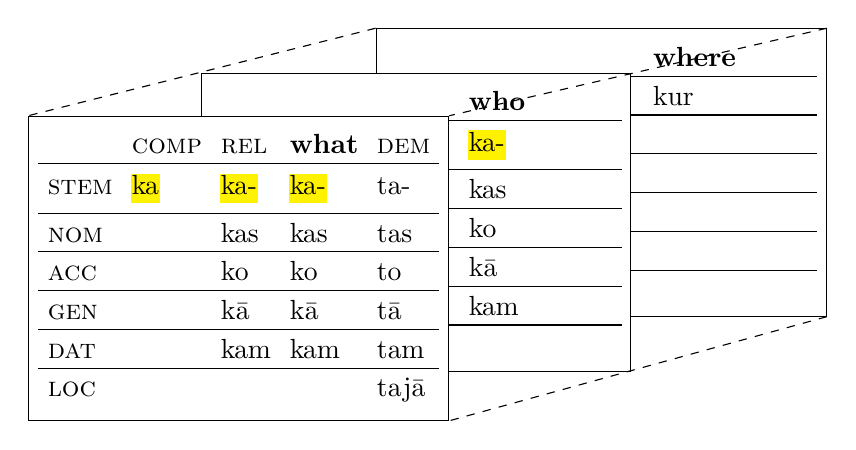
\begin{tikzpicture}[every node/.style={anchor=base west,fill=white,minimum width=0.1cm,minimum height=2mm}]
\matrix (mA) [draw,matrix of math nodes,matrix anchor=north east]
{
& \textsc{{\color{white}comp}} & \textsc{{\color{white}rel}} &[2mm] \textsc{\textbf{where}} & \textsc{{\color{white}dem}} \\\hline
\textsc{{\color{white}stem}}	& {\color{white}0} 	& {\color{white}0} 	& \textup{kur} 	& {\color{white}0}\\\hline
\textsc{nom} 	&  			& \textup{kas} &  & {\color{white}0}\\\hline
\textsc{acc} 	& 			& \textup{ko} 	&   & {\color{white}0}\\\hline
\textsc{gen} 	&  			& \textup{k} &  & {\color{white}0} \\\hline
\textsc{dat} 	&  			& \textup{kam} &  & {\color{white}0} \\\hline
\textsc{loc}	&  			&  &  & {\color{white}0} \\
};

\matrix (mB) [draw,matrix of math nodes,matrix anchor=north east] at ($(mA.south west)+(3.25,3.10)$)
{
& \textsc{{\color{white}comp}} & \textsc{{\color{white}rel}} & [2mm]\textsc{\textbf{who}} & \textsc{{\color{white}dem0}} \\\hline
			&  	&  	& \textup{\hl{ka-}} 	& {\color{white}0}\\\hline
\textsc{nom} 	&  			& \textup{kas} & \textup{kas} & {\color{white}0}\\\hline
\textsc{acc} 	& 			& \textup{ko} 	& \textup{ko}  & {\color{white}0}\\\hline
\textsc{gen} 	&  			& \textup{k}\textup{\={a}} & \textup{k}\textup{\={a}} & {\color{white}0} \\\hline
\textsc{dat} 	&  			& \textup{kam} & \textup{kam} & {\color{white}0} \\\hline
\textsc{loc}	&  			&  &  & {\color{white}00} \\
};

\matrix (mC) [draw,matrix of math nodes,matrix anchor=north east] at ($(mB.south west)+(3.15,3.25)$)
{
& \textsc{comp} & \textsc{rel} 		& \textsc{\textbf{what}} 				& \textsc{dem} \\\hline
\textsc{stem}	& \textup{\hl{ka}} 	& \textup{\hl{ka-}} 	& \textup{\hl{ka-}} 	& \textup{ta-}\\\hline
\textsc{nom} 	&  				& \textup{kas} 		& \textup{kas} 		& \textup{tas}\\\hline
\textsc{acc} 	& 				& \textup{ko} 		& \textup{ko}  		& \textup{to}\\\hline
\textsc{gen} 	&  	& \textup{k}\textup{\={a}} & \textup{k}\textup{\={a}} & \textup{t}\textup{\={a}} \\\hline
\textsc{dat} 	&  				& \textup{kam} 		& \textup{kam} & \textup{tam} \\\hline
\textsc{loc}	&  				&  			&  & \textup{taj}\textup{\={a}} \\
};

\draw[dashed](mA.north east)--(mC.north east);
\draw[dashed](mA.north west)--(mC.north west);
\draw[dashed](mA.south east)--(mC.south east);
\end{tikzpicture}
\end{center}

\noindent Only one of these wh-pronouns, \textit{kas} `what', is a cell in the cross-categorial paradigm (the horizontal coordinate) and both `what' and `who' are inflected for case (the vertical coordinate). The values of the vertical coordinate in \ref{3D} are described by the case fseq in \ref{ver}, the values of the horizontal coordinate by \ref{hor}, and the values of the backward aisle by a decomposition of the (pro)nominal base in \ref{refined-NP}, the subset of the \isi{wh-pronoun}s, repeated below.

\ex. Place\,$>$\,Person\,$>$\,Thing

The ordering of the refined (pro)nominal base with respect to the other fseqs gives us the updated singleton sequence, as in the following:

\ex. \ldots \ $>$\,K$_{3}$P\,$>$\,K$_{2}$P\,$>$\,K$_{1}$P\,$>$\,Comp\,$>$\,Rel\,$>$\,Wh\,$>$\,Dem\textsubscript{indef}\,$>$\,Place\,$>$\\
Person $>$\,Thing

\noindent
If the \isi{*ABA} generalization follows from the \isi{Superset Principle} that applies to an ordered \isi{fseq}, then we correctly expect syncretism to be restricted to adjacent cells in \textit{n}-dimensional \isi{paradigm}s, a result described independently for two-dimensional paradigms earlier in \cite{CahaPantcheva2012} and \cite{GVW2018}. In \ref{3D} we observe the syncretic span restricted to adjacent cells of the horizontal and the backward coordinates that includes the `what'-cell at their juncture.
\par With the decomposition of Dem\textsubscript{indef} into `Dist\,$>$\,Med\,$>$\,Prox', we are able to further refine the singleton sequence of projections as in:

\ex. \ldots \ $>$\,K$_{3}$P\,$>$\,K$_{2}$P\,$>$\,K$_{1}$P\,$>$\,Comp\,$>$\,Rel\,$>$\,Wh\,$>$\,Dist\,$>$\,Med\,$>$\,Prox\,$>$\\ 
Place\,$>$\,Person\,$>$\,Thing

With this refinement in place, the distinction between the \ili{Latvian} proximal \textit{\v{s}is} and the medial/distal \textit{tas} belongs to the third coordinate in the paradigm (the forward aisle), as in \ref{3D:dem}.
\par
 The representation of the Prox \textit{\v{s}is} as a cell forming the third coordinate reflects the fact that both Prox \textit{\v{s}is} and Med/Dist \textit{tas} are case inflected but only the latter is a cell in the cross-categorial paradigm with Comp, Rel, and Wh. 
Such an ordering also captures the observation we can make on the basis of the data discussed so far, namely that proximal \isi{demonstrative}s by and large do not belong to the ``Dem\textsubscript{def}\,$>$\,Comp\,$>$\,Rel\,$>$\,Wh\,$>$\,Dem\textsubscript{indef}'' sequence, the statement which appears to hold both for languages with ``high'' Dem\textsubscript{def}  (e.g. English \textit{that - what} or  Spanish \textit{aqu\'el - qu\'e}) and the ``low'' Dem\textsubscript{indef} (e.g. \ili{Russian} \textit{to - \v{c}to} or \ili{Polish} \textit{to - co}). Though, more typological work is required before this can be turned into a generalization.\pagebreak

\ex.\label{3D:dem}

\begin{center}\vspace{-20pt}
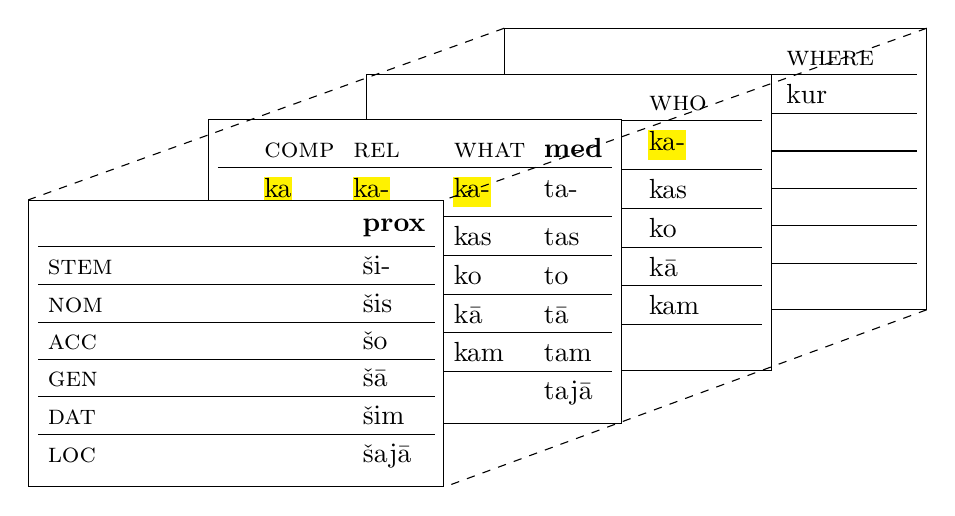
\begin{tikzpicture}[every node/.style={anchor=base west,fill=white,minimum width=0.1cm,minimum height=2mm}]
\matrix (mA) [draw,matrix of math nodes,matrix anchor=north east]
{
\textsc{{\color{white}ooo}} & \textsc{{\color{white}ooo}} & \textsc{{\color{white}ooo}} &[6mm] \textsc{where} & \textsc{{\color{white}0}} \\\hline
{\color{white}ooo}	& {\color{white}ooo} 	& {\color{white}0} 	& \textup{kur} 	& {\color{white}0}\\\hline
 	&  			&  &  & {\color{white}0}\\\hline
 	& 			&  	&   & {\color{white}0}\\\hline
	&  			&  &  & {\color{white}0} \\\hline
 	&  			&  &  & {\color{white}0} \\\hline
	&  			&  &  & {\color{white}0} \\
};

\matrix (mB) [draw,matrix of math nodes,matrix anchor=north east] at ($(mA.south west)+(3.4,3.0)$)
{
& \textsc{{\color{white}comp}} & \textsc{{\color{white}rel}} &[4mm] \textsc{who} & \textsc{{\color{white}0}} \\\hline
{\color{white}ooo}	&  	&  	& \textup{\hl{ka-}} 	& {\color{white}0}\\\hline
\textsc{nom} 	&  			& \textup{kas} 	& \textup{kas} 		& {\color{white}0}\\\hline
\textsc{acc} 	& 			& \textup{ko} 	& \textup{ko}  		& {\color{white}0}\\\hline
\textsc{gen} 	&  			& \textup{k}\textup{\={a}} 	& \textup{k}\textup{\={a}} & {\color{white}0} \\\hline
\textsc{dat} 	&  			& \textup{kam} & \textup{kam} 		& {\color{white}0} \\\hline
\textsc{loc}	&  			&  &  & {\color{white}00} \\
};

\matrix (mC) [draw,matrix of math nodes,matrix anchor=north east] at ($(mB.south west)+(3.25,3.2)$)
{
& \textsc{comp} & \textsc{rel} 			&[4mm] \textsc{what} 	& \textsc{\textbf{med}} \\\hline
	& \textup{\hl{ka}} 	& \textup{\hl{ka-}} 	& \textup{\hl{ka-}} 	& \textup{ta-}\\\hline
\textsc{n} 	&  					& \textup{kas} 		& \textup{kas} 		& \textup{tas}\\\hline
\textsc{a} 	& 					& \textup{ko} 		& \textup{ko}  		& \textup{to}\\\hline
\textsc{g} 	&  & \textup{k}\textup{\={a}} & \textup{k}\textup{\={a}} & \textup{t}\textup{\={a}}\\\hline
\textsc{d} 	&  					& \textup{kam} 		& \textup{kam} 		& \textup{tam} \\\hline
\textsc{i}	&  			&  		&  				& \textup{taj}\textup{\={a}} \\
};

\matrix (dem) [draw,matrix of math nodes,matrix anchor=north east] at ($(mC.south west)+(3,2.85)$)
{
& {\color{white}ooooo} & {\color{white}oooo} & {\color{white}oooo} 				& \textsc{\textbf{prox}} \\\hline
\textsc{stem}	& {\color{white}oooo} & {\color{white}oooo} & {\color{white}oooo} 	& \textup{\v{s}i-}\\\hline
\textsc{nom} 	&  			&   		&   								& \textup{\v{s}is}\\\hline
\textsc{acc} 	& 			&  		&   								& \textup{\v{s}o}\\\hline
\textsc{gen} 	&  			& 		&  					& \textup{\v{s}}\textup{\={a}}\\\hline
\textsc{dat} 	&  			&  		&  								& \textup{\v{s}im} \\\hline
\textsc{loc}	&  			&  		&  					& \textup{\v{s}aj}\textup{\={a}} \\
};


\draw[dashed](mA.north east)--(dem.north east);
\draw[dashed](mA.north west)--(dem.north west);
\draw[dashed](mA.south east)--(dem.south east);
\end{tikzpicture}
\end{center}


 
\section{Summary}

The inclusion of the indefinite \isi{demonstrative} pronoun as the bottom category in an \isi{fseq} which covers \isi{syncretism}s with the declarative \isi{complementizer} allowed us to explain morphological \isi{containment} and syncretic alignment in such a \isi{paradigm} in \ili{Slavic}. The same holds true for \ili{Latvian}, too, which enabled us to describe the paradigm with the Comp \textit{ka}, the only suffixless item in  the fseq in \Next,  as a caseless category in a sequence where case marking is delimited by Rel. 

\ex. Comp\,$>$\,Rel\,$>$\,Wh\,$>$\,Dem\textsubscript{indef}

\noindent
Such a result follows naturally from the representation of these morphologically complex categories as a singleton sequence of syntactic projections, whose segregation into more complex subtrees is exclusively an effect of the \isi{spell-out} procedure, not of the complexity of an underlying syntactic representation.
One consequence of that approach is a possibility to describe multi-dimensional \isi{paradigm}s as a single homeomorphic sequence of syntactic projections, a conjecture shown to hold for a three-dimensional \isi{paradigm} in \ili{Latvian}.



 
\chapter{An apparent *ABA violation in Basa\'a}\label{chapter:basaa}

\section{Introduction: an ABA paradigm}

The inclusion of Dem\textsubscript{indef} as the bottom of the hierarchy in \ref{reiteratedfseq} proposed in Chapter \ref{chapter:resolving} constitutes an essential ingredient of sorting out what appears to be an ABA pattern of \isi{syncretism} in \ili{Basa\'a} (\ili{Bantu}, A.43). \is{fseq}

\ex.\label{reiteratedfseq} 
Dem\textsubscript{def}\,$>$\,Comp\,$>$\,Rel\,$>$\,Wh\,$>$\,Dem\textsubscript{indef} \hfill (reiterated)

Namely, as shown in \tabref{ABA:Basaa}, the \ili{Basa\'a} \isi{paradigm} shows a Dem$=$Rel syncretism to the exclusion of Comp.

\begin{table}
\caption{Basa\'a}
\label{ABA:Basaa}
\begin{tabular}[t]{ l l l l l l }
\lsptoprule
\textsc{dem} 	& \textsc{comp} 	& \textsc{rel}  	& \textsc{wh}\\	
\midrule
n\'u\cellcolor[gray]{0.9} & $\emptyset$, & n\'u,\cellcolor[gray]{0.9} & k\'i\'i\\
 & lέ\cellcolor[gray]{0.8} & lέ\cellcolor[gray]{0.8} & \\
\lspbottomrule
\end{tabular}
\end{table}

\noindent The arrangement of the cells in the \ili{Basa\'a} \isi{paradigm}  in the same way as in the Germanic languages, as for instance in \ili{English}, \ili{Dutch}, German or \ili{Swiss German} in \tabref{table:no-wo} (partially repeated from \sectref{sec:paradajm}), results in the violation of the \isi{*ABA} generalization.

\begin{table}
\caption{Germanic}
\label{table:no-wo}
\begin{tabular}[t]{ l l l l l l }
\lsptoprule
& \textsc{dem} 	& \textsc{comp} 	& \textsc{rel}  	& \textsc{wh}\\	
\midrule
English & that\cellcolor[gray]{0.9} & that\cellcolor[gray]{0.9} & that\cellcolor[gray]{0.9} & what\\
Dutch & dat\cellcolor[gray]{0.9} & dat\cellcolor[gray]{0.9} & dat\cellcolor[gray]{0.9} 	& wat\\
German & das\cellcolor[gray]{0.9} & dass\cellcolor[gray]{0.9} & das\cellcolor[gray]{0.9} & was\\
Swiss German & das\cellcolor[gray]{0.9} & dass\cellcolor[gray]{0.9} & $\emptyset$ & was\\ 
\lspbottomrule
\end{tabular}
\end{table}

\noindent The description of the \ili{Swiss German} relative pronoun as the phonologically null marker in \tabref{table:no-wo} requires qualification, which shows a direction toward working out a solution for the refractory \ili{Basa\'a} \isi{paradigm} in \tabref{ABA:Basaa}.

\subsection{Excursus on the Rel-cell in Swiss German}

In \ili{Swiss German}, an invariant particle \textit{wo} introduces both locative relatives, as in \ref{wo-loc}, and headed relative clauses, as in \ref{wo-hr}. It is syncretic with the locative `where'.

\ex. \ili{Swiss German} (\citealt[ex. 42a,b]{vanR2003})
\ag. 
s huss wo de Hans wont\\
the house \textsc{wo} the Hans lives\\
\strut `the house where Hans lives'\label{wo-loc}
\bg.
s f\"ascht wo i gh\"o\"ort han das de Hans anegaat\\
the party \textsc{wo} I heard have that the Hans to.goes\\
\strut `the party that I have heard Hans is going to' \label{wo-hr}

However, \citeauthor{vanR1989} (\citeyear{vanR1989}, \citeyear{vanR2003}) shows that \textit{wo} is not a genuine \isi{relativizer} despite the fact that headed relatives in \ili{Swiss German} are never preceded by a distinct relative pronoun. We can see this, among others, when we compare \ili{Swiss German} with certain other \ili{Upper German dialects} where \textit{wo} either can or must be preceded by a relative \textit{d}-pronoun (see also \citealt{Salzmann2006} and \citealt{BB}).
This is shown in the following examples contrasting \ili{Bavarian} with \ili{Swiss German} (more precisely, the \ili{Z\"urit\"u\"utsch dialect}):

\ex. \ili{Bavarian} (\citealt[216]{Bayer1984})
\ag.[]\hspace{-22pt}I schenk 's dem Kind (des) wo mid da Katz spuid.\\
\hspace{-22pt}I give it the.\textsc{dat} child {\ }\textsc{rel} \textsc{wo} with the cat plays\\
\hspace{-22pt}\strut `I give it to the child that plays with the cat.' 


\ex. \ili{Swiss German} - Z\"urit\"u\"utsch (\citealt[4]{vanR2003}) 
\ag.[]\hspace{-22pt}I sch\"ank 's em chind (*das) wo mit de chatz spilt.\\
\hspace{-22pt}I give it the.\textsc{dat} child {\ \ }\textsc{rel} \textsc{wo} with the cat plays\\
\hspace{-22pt}\strut `I give it to the child that is playing with the cat.' 

The \textit{d}-pronoun strongly appears to qualify as a genuine \isi{relativizer} (in the sense that it belongs to the cross-categorial \isi{paradigm} with the declarative Comp).
\par
The contrast illustrated above, however, begs a question why \textit{wo}-relatives come with a relative pronoun in dialects like \ili{Bavarian} but not in \ili{Swiss German}. 
There is more than one possibility, including an analysis advanced in \citet{PennerBader1995} where it is argued on the basis of the \ili{Bernese dialect} of \ili{Swiss German} that the relative pronoun is a silent \textit{pro}. Also, an interesting insight about \textit{wo}-relatives in the \ili{Z\"urit\"u\"utsch dialect} is offered in \citet{vanR2003}, who argues that they are similar to the so-called aboutness `such that' relatives, which are found in \ili{Japanese} (\citealt[257]{Kuno1973}) and also in \ili{English} (\citealt[157]{Grosu2002}), as in \textit{A mathematical system such that two and two are four is Peano arithmetic}. If on the right track, this account further speaks against classifying \textit{wo} as a relative pronoun.
\par
While working out the right analysis of the \textit{wo}-relatives is a task of its own, what is important for the purposes of the data classification is that \textit{wo} is not a relative pronoun on par with \textit{das} and must therefore be kept separate from the \isi{paradigm} in \tabref{table:no-wo} in a similar way verbal \isi{complementizer}s are kept separate form the paradigm with the nominal complementizer (as for instance in Yoruba or Hausa as seen in (\pref{Yoruba}--\pref{Hausa}) in \sectref{sec:paradajm}).
\par
The point of this observation is that while describing the \ili{Swiss German} relative pronoun either as $\emptyset$ or \textit{wo} does not have consequences for syncretic alignment as neither form shows \isi{syncretism} with the remaining three categories in \tabref{table:no-wo}, the examination of the syntax behind the Dem-cell in \ili{Basa\'a} is going to inform us about the solution to the \isi{*ABA} problem. 

\subsection{Back to the Basa\'a paradigm} 

Perhaps an immediate attempt to resolve the \isi{*ABA} violation in \tabref{ABA:Basaa} is to assume that since the \isi{complementizer} that appears to disrupt the syncretic span between Dem and Rel is phonologically null, then the Comp layer is not projected in \ili{Basa\'a} at all. Such an explanation is challenged by the fact that a dialect of \ili{Basa\'a} does have an overt form of the declarative complementizer \textit{lέ}, as shown in: 

\ex. \ili{Basa\'a} (\citealt[ex. 30a in \S3]{Bassong2010})\label{bassong-ch3}
\ag.[]\hspace{-22pt}mɛ ŋ́-k\^al lέ Tonye a ŋ́-kŋ́ y\`a\'an\'i\\
\hspace{-22pt}I \textsc{pres}-say \textsc{comp} Tomye \textsc{sm} \textsc{pres}-go tomorrow\\
\hspace{-22pt}\strut `I say that Tonye will go tomorrow.'

This variant of the \isi{complementizer} is syncretic with the relativizer, as in shown in the following:\largerpage

\ex. Basa\'a (\citealt[ex. 22b in \S4]{Bassong2010})\label{le-rel}
\ag.[]\hspace{-22pt}ɓa\'ud\'u ɓ\'a gw\v{e} mal\v{e}t lέ a ŋ́-k\^al ɓɔ́ mam\\
\hspace{-22pt}students \textsc{sm} have teacher \textsc{rel} \textsc{sm} \textsc{pres-}tell them things\\
\hspace{-22pt}\strut `The students have a teacher that tells them stories.' 

According to Bassong, the \isi{relativizer} \textit{lέ} is indeclinable and its distribution in \isi{relative clause}s is more restricted than in the case of \textit{n\'u}. An intuitive option would be, thus, to further assume that Comp is a layer of structure that can be skipped -- but only on top of the \isi{paradigm} with the Rel \textit{n\'u} and not on top of the paradigm with the Rel \textit{lέ}. The liaison of these two assumptions, however, is unnecessary if the \ili{Basa\'a} demonstratives are indefinite since, as argued earlier, only definite demonstratives of the type found in Germanic languages are the categories that are structurally bigger than declarative complementizers and \isi{relativizer}s. 
\par
In what follows, I consider a wholesale different approach to resolving the  \isi{*ABA} problem in  \ili{Basa\'a}, the one which relies on inspecting the syntax of the categories behind the Dem and Rel cells in the offending paradigm in \tabref{ABA:Basaa}.

\section{Basa\'a demonstratives}

The first step toward resolving this problem involves contrasting the demonstrative \textit{n\'u} with the Germanic demonstratives and classifying it as the smallest rather than the biggest category in the ``Dem\textsubscript{def}\,$>$\,Comp\,$>$\,Rel\,$>$\,Wh\,$>$\,Dem\textsubscript{indef}'' sequence. The classification of the demonstrative \textit{n\'u} as indefinite, however, requires qualification since \ili{Basa\'a} does have morphological marking of specificity.
\par
 Let us consider the following. \ili{Basa\'a} demonstratives show noun class concord with the noun they apply to. The demonstratives are morphologically distinguished between the proximal (close to speaker), the medial (close to hearer), and the distal (far from speaker and hearer), as shown on the example of class 1 \textit{n\'u} and class 5 \textit{l\'i} below (examples \pref{smierc}--\pref{Bas:liwanda}) are from \citealt{Makasso2010}).\footnote{See \cite{Hyman2003} for an exhaustive list of demonstratives of all nominal classes in \ili{Basa\'a}.
} %end of fn

\ex.\label{smierc} 
\ag. \{ l\'in\'i / l\'i / {l\'i\'i \}} liw\'and\'a \\
 {} 5.\textsc{prox} {} 5.\textsc{med} {} {5.\textsc{dist}} 5.friend\\
\strut `this/that friend'
\bg. \{ n\'un\'u / n\'u / {n\'u\'u \}} mut \\
 {} 1.\textsc{prox} {} 1.\textsc{med} {} {1.\textsc{dist}} 1.person\\
\strut `this/that person'

\noindent In \ili{Basa\'a}, the demonstratives can appear before or after the nouns they modify. Pre-nominal demonstratives receive a focus interpretation, while a noun that is post-modified by a demonstrative is unmarked with respect to information structure (non-focus) and it is obligatorily prefixed with the augment \textit{\'i-}, which marks definiteness/specificity (\citealt{Jenks-etall}), as shown in the following: \is{morpheme}

\ex.\label{Bas:i}
\ag.
\textbf{\'i}-mut\textsubscript{1} n\'u\\
\textsc{aug}-1.person 1.that.\textsc{dem}\\
\strut `that person' 
\bg.
n\'u mut\\
1.that.\textsc{dem} 1.person\\
\strut `THAT person'\label{B:unprefixednoun} 

\noindent
This description holds for all classes of demonstratives and for all values of the proximal-medial-distal contrast:

\ex. \label{Bas:liwanda}
\ag. \{ l\'in\'i / l\'i / {l\'i\'i \}} liw\'and\'a \\
 {} 5.\textsc{prox} {} 5.\textsc{med} {} {5.\textsc{dist}} 5.friend\\
\strut `this/that friend'
\bg.  l\textbf{\'i\textsuperscript{↓}}-w\'and\'a \{ l\'in\'i / l\'i / {l\'i\'i \}}\\
 \textsc{aug.}-5.friend  {} 5.\textsc{prox} {} 5.\textsc{med} {} {5.\textsc{dist}}\\
\strut `this/that friend'

Since these demonstratives do not have definiteness morphology, we can classify them as indefinite on par with \ili{Russian}, \ili{Polish}, \ili{Czech}, and \ili{Latvian} demonstratives. What sets the \ili{Basa\'a} demonstratives apart from the latter is that, descriptively speaking, the first participate in contextual licensing of an augment prefix on the noun they modify, but other than that there is no trace of the Def ingredient in their structure that qualifies them as the biggest category in the sequence in \ref{reiteratedfseq}. \is{morpheme} \is{fseq}
\par
However, the fact that we are able to accommodate indefinite demonstratives as the smallest category in this sequence, which results in the reordering of the cells as in \tabref{table3}, does not resolve the \isi{*ABA} problem but merely pushes it to a different place of the \isi{paradigm} where the non-syncretic Wh is now sandwiched between the syncretic forms for Rel and Dem\textsubscript{indef}. \is{syncretism}

\begin{table}
\caption{Reordered paradigm in Basa\'a}
\label{table3}
\begin{tabular}[t]{ l l l l l l }
\lsptoprule
\textsc{dem}\textsubscript{def} & \textsc{comp} 	& \textsc{rel}  	& \textsc{wh} & \textsc{dem}\textsubscript{indef}\\	
 \midrule
& $\emptyset$, & n\'u,\cellcolor[gray]{0.9} & k\'i\'i  & n\'u\cellcolor[gray]{0.9}\\
& lέ\cellcolor[gray]{0.8} & lέ\cellcolor[gray]{0.8} & \\
\lspbottomrule
\end{tabular}
\end{table}

\section{Non-wh-relatives in Basa\'a}

The key to resolving this problem is the observation that a similar distribution between the  augment \textit{\'i}-prefix on the head noun and a demonstrative pronoun we see in (\pref{Bas:i}--\pref{Bas:liwanda}) holds in headed \isi{relative clause}s, too, with the one essential difference: the augment \textit{\'i}-prefix is optional in relative clauses.
\par 
In both subject and object \isi{relative clause}s in \ili{Basa\'a}, the medial demonstrative pronoun is the one which shows \isi{syncretism} with the relative pronoun. This is  shown below on the example of class 1 medial \textit{n\'u}.

\ex. \citet[153--4]{Makasso2010}\label{Bas:big}
\ag. 
mɛ ŋ́ gwέs m\^ut\textsubscript{i} (n\'u)  [ \_\textsubscript{i}  a y\'e mb\'om ] \\
I \textsc{pres} like 1.person 1.\textsc{rel} {} {} 1.\textsc{sbj} \textsc{cop} 9.big\\
\strut `I like a person that is big/important.' 
\bg. 
mɛ \'n y\'eŋ m\'a\'aŋgέ\textsubscript{i} (n\'u) [ mɛ \'n y\'i \_\textsubscript{i} ]\\
\textsc{1sg} \textsc{pres} seek 1.child \textsc{1.rel} {} \textsc{1sg} \textsc{pr} know\\
\strut `I'm looking at the child that I know.' 

As pointed out in \citet{Makasso2010}, while the augment \textit{\'i}- is obligatory on nouns post-modified by demonstratives, it is optional on nouns that are heads of relative clauses, as shown in \Next, in which case the noun phrase is interpreted as indefinite.

\ex.
\ag.
(\textbf{\'i})-mut\textsubscript{i} n\'u [ \_\textsubscript{i} a b\'i \textsuperscript{↓}jέ b\'ijέk ]\\
\textsc{aug}-1.person 1.\textsc{rel} {} {} \textsc{1.sbj} \textsc{pst} eat 8.food {}\\
\strut `that person that ate the food'\label{RelC:i}
\bg.
n\'u (*\textbf{\'i})-mut\textsubscript{i} [ \_\textsubscript{i} a b\'i \textsuperscript{↓}jέ b\'ijέk ]\\
1.that \textsc{aug}-1.person {} {} \textsc{1.sbj} \textsc{pst} eat 8.food\\
\strut `THAT person that ate the food'\label{RelC:senza-i}


\noindent A two-step analysis of relativization in \ili{Basa\'a} which covers these facts is put forward in \cite{Jenks-etall}, whose central ingredient of the solution the \isi{*ABA} problem involves the derivation of the pre-nominal placement of the demonstrative in the noun phrase from its post-nominal placement, as outlined in \ref{DFCF}.

 \ex.\label{DFCF}
\setlength{\arrowht}{3ex}
\newcommand*\cgdepthstrut{{\vrule height 0pt depth \arrowht width 0pt}}
\renewcommand\eachwordone{\cgdepthstrut\rmfamily}
\renewcommand\glt{\vskip -\topsep}
\let\trans=\glt
\newcommand\arrowex{\setlength{\arrowht}{1ex}\ex}
[\textsubscript{DP} \tikzmark{n}\'u\textsubscript{Dem} (*\textbf{\'i}-) [\textsubscript{NP} mut ]  \tikzmark{t}  ]
 \arrow{t}{n}

\vskip 0.45cm
Such a derivation captures the complementary distribution between the augment marker \textit{\'i-} and the pre-nominal demonstrative in terms of blocking. Specifically, in
 \citeauthor{Jenks-etall}'s \citeyearpar{Jenks-etall} account this instantiates a ``generalized Doubly-filled Comp Filter'' (DFCF), whereby either a head or its specifier can be lexically realized. For \ref{DFCF} it means that \textit{\'i-} in the D-head position cannot be lexicalized when the demonstrative moves to its specifier from a post-nominal position. The analysis advanced here does not depend on the explanation based on a generalized DFCF, instead, it is enough for us to observe that the fronting of Dem blocks the merger of the augment marker. 
\par
The other ingredient of \citeauthor{Jenks-etall}'s \citeyearpar{Jenks-etall} account involves the derivation of \isi{relative clause}s in \ili{Basa\'a} via head raising in the way advanced in \cite{Kayne1994}. Let us note that such an approach to the relative clause formation is in agreement with what has been argued for other \ili{Bantu} languages (see e.g. \citealt{Ngonyani2001} and \citealt{Carstens2005}). 
\par
In \citeauthor{Kayne1994}'s \citeyearpar{Kayne1994} analysis, the head nouns are merged as specifiers of the \isi{relative clause}, which can be selected by the D-head.
 This gives us the following result for the derivation of headed relative clauses (labelled as RelP in the derivations below) with the pre-nominal demonstrative in \ili{Basa\'a}.

\ex. Derivation of a \isi{relative clause} with a post-nominal demonstrative following \citet[34]{Jenks-etall}
\ag.\'i-mut\textsubscript{i} n\'u [ \_\textsubscript{i} a b\'i \textsuperscript{↓}jέ b\'ijέk ]\label{optionalnu} \\
\textsc{aug}-1.person 1.\textsc{rel} {} {} \textsc{1.sbj} \textsc{pst} eat 8.food {}\\
\strut `that person that ate the food'
\b.\label{nu1} 
\begin{forest}nice empty nodes, for tree={l sep=0.6em,l=0,calign angle=63}
[DP$_{1}$, s sep=-10pt [D$_{1}$ [\textit{\'i}]]
 [RelP, s sep=15pt  [DP$_{2}$, name=tgt , s sep=15pt  
 [NP [\textit{mut}, name=tgt2, roof]][{}, s sep=15pt [Op [\textit{n\'u}, roof]]
 [{} [D$_{2}$ [$\emptyset$]][\dots, name=t2]]]]
 [{}, s sep=15pt
 [Rel [$\emptyset$]] [TP [\dots, name=t]
 [T' [\textit{a b\'i \textsuperscript{↓}jέ b\'ijέk}, roof]]]]]]
 \draw[dashed,->,>=stealth,overlay] (t2) ..controls +(south:1.75) and +(south:1.75).. (tgt2);
 \draw[dashed,->,>=stealth,overlay] (t) [in=-155,out=-125,looseness=2.85]  to (tgt);
\end{forest}

\pagebreak\noindent In the first step of this derivation, the noun phrase \textit{mut} `person' is fronted to a position before the \isi{demonstrative} \textit{n\'u} in its own DP$_{2}$ (described as the ``Op(erator)'' position in \citealt{Jenks-etall}).\footnote{\cite{Jenks-etall} follow \cite{Kayne1994} in labelling the relative clauses simply as CP. RelP is used instead in the diagrams below in order to disambiguate the head of the \isi{relative clause}, Rel, with the head of the clause headed by a \isi{complementizer}, Comp, as these are structurally distinct categories in the strand of research we explore in the present work. This is a technical remark with no consequences for the constituent structure of relative clauses or for the essence of \citeauthor{Jenks-etall}'s \citeyearpar{Jenks-etall} analysis.
} %end of fn
 In the second step, the entire DP$_{2}$ is fronted to the specifier of RelP. The augment marker \textit{\'i}-  spells out the top selecting head D$_{1}$ and comes out as the prefix on the head noun \textit{mut}.
\par 
In \citeauthor{Jenks-etall}'s \citeyearpar{Jenks-etall} account, the post-nominal ``operator'' position of the \isi{demonstrative} does not receive a focus reading when the DP$_{2}$ is in the specifier of the relative clause. In contrast, in the derivation of \isi{relative clause}s with a pre-nominal \textit{n\'u}, the \textit{n\'u} is a genuine demonstrative rather than the ``operator''. In this case, the entire relative DP$_{2}$ is raised out of RelP to a higher position where the demonstrative \textit{n\'u} receives a focus reading, as outlined in \ref{ozzy}.

\ex.\label{ozzy} 
Derivation of a \isi{relative clause} with a pre-nominal \isi{demonstrative} following \citet[35]{Jenks-etall}
\ag.
n\'u mut\textsubscript{i} [ \_\textsubscript{i} a b\'i \textsuperscript{↓}jέ b\'ijέk ]\\
1.that 1.person {} {} \textsc{1.sbj} \textsc{pst} eat 8.food\\
\strut `THAT person that ate the food'\medskip
\b.\label{nu2} 
\begin{forest}nice empty nodes, for tree={l sep=0.7em,l=0,calign angle=63}
 [DP$_{1}$, s sep=20pt  [DP$_{2}$, , s sep=10pt, name=Z
 [Dem [\textit{n\'u}, roof]][{}[D$_{2}$, s sep=12pt [$\emptyset$]][NP [\textit{mut}, roof]]]]
 [{}, s sep=20pt [D$_{1}$ [$\emptyset$]][RelP, s sep=15pt [\dots, name=tgt ][, s sep=10pt [Rel [$\emptyset$]][TP [\dots, name=t]
 [T' [\textit{a b\'i \textsuperscript{↓}jέ b\'ijέk}, roof]]]]]]]]
  \draw[dashed,->,>=stealth,overlay] (t) ..controls +(south west:2) and +(south west:1.5).. (tgt);
   \draw[dashed,->,>=stealth,overlay] (tgt) ..controls +(south west:6) and +(west:3.5).. (Z);
\end{forest}

A particularly telling argument in support of such an analysis is that it accounts for the complementary distribution between demonstratives and what (appears to be) a separate relativizer in all types relative clauses involving a gap. The relative clauses involving a gap are subject and object relatives with pre- and post-nominal demonstratives. These are shown in the following:
 
\exg.
\textbf{\'i}-maaŋgέ\textsubscript{i} n\'u (*n\'u) [ mɛ \'n y\'i \_\textsubscript{i} ]\\
\textsc{aug}-1.child {1.\textsc{dem}} \phantom{X}\textsc{1.rel} {} \textsc{1sg} \textsc{pres} know\\
\strut `this/that child that I know'

\exg.
l\'i l\'i-w\'and\'a\textsubscript{i} (*l\'i\textsuperscript{↓}) [ \_\textsubscript{i} l\'i b\'i \textsuperscript{↓}jέ b\'ijέk ] \\
5.\textsc{dem} 5-friend \phantom{X}\textsc{5.rel} {} {} \textsc{5.sbj} \textsc{pst} eat food\\
\strut `THAT friend that ate the food' 

Such a complementary distribution of the medial \isi{demonstrative} pronoun and the relativizer in \isi{relative clause}s involving a gap shows that the relation between these two categories in \ili{Basa\'a} is robust and hence the problematic Dem=Rel \isi{syncretism} to the exclusion of Wh cannot be attributed to an accidental homophony. 
\par
If we follow \citeauthor{Jenks-etall}'s \citeyearpar{Jenks-etall} analysis of the formation of non-wh-relatives in \ili{Basa\'a}, we can directly resolve the \isi{*ABA} problem  present in \tabref{table3}. 
The juxtaposition of the syntax of non-wh-relatives in \ili{Basa\'a} with the syntax of non-wh-relatives in languages like \ili{English} reveals  that the second involves a genuine \isi{relativizer}, which does not form a constituent with the head noun, as outlined by the following example:

\ex. 
\a. the person that found our cat\medskip
\b.
\begin{forest}nice empty nodes, for tree={l sep=0.65em,l=0,calign angle=63}
[DP$_{1}$, s sep=15pt [D$_{1}$ [\textit{the}]]
 [RelP, s sep=20pt  [NP, name=tgt [\textit{person} ,  roof]]
 [{}, s sep=10pt
 [Rel [\textit{that}, roof]] [TP [\dots, name=t]
 [T' [\textit{found our cat}, roof]]]]]]
\draw[dashed,->,>=stealth] (t) [in=-150,out=-125,looseness=1.75]  to (tgt);
\end{forest}

\vskip -0.75cm
\noindent
This contrasts with the \ili{Basa\'a} \textit{n\'u}, which comes out as a genuine \isi{demonstrative} pronoun, which forms a constituent with the head noun. In turn, the relativizer, understood as the head of the relative clause, is null. This result requires the problematic \isi{paradigm} in \ili{Basa\'a} to be rewritten as in \tabref{table4}, which removes the \isi{*ABA} violation with the demonstrative and keeps the syncretic span Comp=Rel in the parallel paradigm with \textit{lέ}.

\begin{table}
\caption{Final version of the Basa\'a paradigm}
\label{table4}
\begin{tabular}[h]{ l l l l l l }
\lsptoprule
\textsc{dem}\textsubscript{def} & \textsc{comp} 	& \textsc{rel}  	& \textsc{wh} & \textsc{dem}\textsubscript{indef}\\	
\midrule
 & $\emptyset$\cellcolor[gray]{0.9}, & $\emptyset$\cellcolor[gray]{0.9}, & k\'i\'i  & n\'u\\
   & lέ\cellcolor[gray]{0.8} & lέ\cellcolor[gray]{0.8} & \\
\lspbottomrule
\end{tabular}
\end{table}

\noindent
The reanalysis of the \isi{paradigm} with a zero relativizer allows us to correctly predict that it will be able to cooccur with elements other than the demonstrative -- class 1 \textit{n\'u} or any other -- in the D head of the \isi{relative clause}. For instance, treating the \ili{English} \textit{that} as a \isi{relativizer}, the head of the relative clause does not need a \isi{demonstrative}, as in:

\ex. John saw \{ three men\slash somebody \} that Mary had fired.

Indeed, as already indicated in the example of a relative clause with a post-nominal demonstrative in \ref{optionalnu}, the null \isi{relativizer} can cooccur with the D head of the \isi{relative clause} that is lexicalized as the \textit{\'i}- prefix.  More generally, as already seen in \ref{Bas:big}, \textit{n\'u} can be generally dropped in both subject and object relative clauses. This optionality holds also with other nominal classes  as shown in the following example from \citet[18]{Jenks-etall}:

\exg. 
h\'inun\'i\textsubscript{i} (h\'i) [ liw\'and\'a l\'i b\'i \textsuperscript{↓}tέhɛ̌  \_\textsubscript{i} ]\\
\textsc{aug}.19.bird \textsc{dem} {} 5.friend 5.\textsc{sbj} \textsc{pst} see \\
\strut `the bird that the friend saw'



\section{Resumptive \isi{relative clause}s}

 A final comment about the \ili{Basa\'a} relative clauses involving resumption is in order. Resumptive relative clauses provide a circumstantial argument that supports both the idea that \isi{relativizer}s in \ili{Basa\'a} are genuine \isi{demonstrative}s as well as the conjecture made earlier on the basis of Slavic, Germanic, and \ili{Latvian} that it is specifically the medial demonstratives that serve as the base category in the  sequence in \ref{reiteratedfseq}.\footnote{The argument is circumstantial in the sense that it depends on a particular analysis of the formation of relative clauses that involve resumption (see for instance \citeauthor{Bianchi2004} \citeyear{Bianchi2004,Bianchi2011} or \citealt[chapters 2--3]{Salzmann2017}).
} %end of fn on resumption
\par
Namely, the complementarity between the \isi{demonstrative} pronoun and (what appears to be a distinct) relativizer is more limited with \isi{relative clause}s that involve resumption. In this environment, it is only the medial demonstrative that cannot co-occur with the relativizer, while the non-syncretic proximal and distal demonstratives can co-occur with the \isi{relativizer}, as shown in the example of object of comparison relative clauses in \ref{tyrionwilldie}.

\ex.\label{tyrionwilldie} Resumptive (object of comparison) \isi{relative clause} (\citealt[27]{Jenks-etall})
\ag.\'i-maaŋgέ\textsubscript{i} \{ n\'un\'u / *n\'u / {n\'u\'u \}} (n\'u) [ ŋgwɔ́ i ye ikέŋ\'i ilέl {ŋyέ\textsubscript{i} ]}\\
\textsc{aug}-1.child {} 1.\textsc{prox} {} \phantom{t}\textsc{1.med} {} {1.\textsc{dist}}
\phantom{l}\textsc{1.rel} {} 9.dog 9.\textsc{sbj} be 9.big exceed {1.\textsc{pron}}\\
\bg.  \{ n\'un\'u / *n\'u / {n\'u\'u \}} maaŋgέ\textsubscript{i} (n\'u) [ ŋgwɔ́ i ye ikέŋ\'i ilέl {ŋyέ\textsubscript{i} ]}\\
 {} 1.\textsc{prox} {} \phantom{t}\textsc{1.med} {} {1.\textsc{dist}} 1.child \phantom{t}\textsc{1.rel} {} 9.dog 9.\textsc{sbj} be 9.big exceed {1.\textsc{pron}}\\
\strut `this/that child that the dog is bigger than' 

This restriction is hard to account for if the \isi{relativizer} is not a genuine \isi{demonstrative} pronoun in the \ili{Basa\'a} relative clauses given that it must show class concord with the head noun, unlike the genuine relativizer \textit{lέ}, as shown in \ref{le-rel}.

\section{Summary}

The resolution of what comes out as an apparent ABA pattern  in the \ili{Basa\'a} \isi{paradigm} is possible if we inspect the syntax behind the offending Rel-cell, in a similar way the description of \textit{wo}-relatives in \ili{Swiss German} indicates that \textit{wo} is not on a par with relative pronouns like the German \textit{das} or the \ili{English} \textit{that}. Specifically, if we follow the analysis of non-wh-\isi{relative clause}s in \ili{Basa\'a} in \cite{Jenks-etall}, the offending relative pronoun turns out to be a genuine DP-internal \isi{demonstrative} that is placed after the head noun. We end up with a picture where overt realization of the cross-categorial paradigm is restricted in \ili{Basa\'a} to its two adjacent cells, in agreement with the \isi{*ABA} generalization and the proposal to insert indefinite \isi{demonstrative}s as the bottom category of the ``Dem\textsubscript{def}\,$>$\,Comp\,$>$\,Rel\,$>$\,Wh\,$>$\,Dem\textsubscript{indef}'' sequence.




 
\chapter{Overview}\label{chapter:conclusion}

\section{Summary}

In the broad sense, I have investigated the nature of the relation between the lexical (linear) and the syntactic (hierarchical) structure in an approach to grammatical representations that keeps up with ongoing work on structuralization of the semantics of lexical items. The results discussed here contribute to the picture that has been getting clearer and clearer for over ten years now which shows that the three descriptive domains\,---\,morphology, lexical semantics, and syntax\,---\,form a single module of grammar as they operate on the same class of features, like [person], [place], [proximal], [definite], etc.
\par
Such a scenario has two immediate consequences for our understanding of the interface between syntax and the lexicon.  One is that morphological structures come out as linear realizations of syn-sem representations \is{linearization} which are seamless with respect to the grammatical \isi{feature}s. In other words, a \isi{morpheme} does not have any more or any fewer features than a syntactic tree it lexicalizes. \is{spell-out} The other one is that a lexicon of a language stores syntactic subtrees paired with their exponents (a view that implies that there is no such thing as a pre-syntactic lexical storage). Following the research program outlined in \citeauthor{Starke2009} (\citeyear{Starke2009,StarkeLA}), both these consequences have been discussed for a few empirical domains in recent years and, in the broad sense, this contribution merely adds up to the growing body of work produced in a similar vein. \is{Nanosyntax}
\par
In the narrow sense, I have investigated a spell-out procedure whereby an ordered set of grammatical operations facilitates the  lexicalization of syntactic structures in a way that allows us to predict exactly (i) how many morphemes a given sequence of syntactic heads is going to be realized by and (ii) what positions these morphemes are going to take (``pre-'' vs. ``post-'' placement). Specifically, I have examined an  alternation in the domain of \ili{Slavic} verbs which exhibits a  reduction in the number of affixes on the root and considered prospects to derive this \isi{reduction} by adding \isi{subextraction} to the existing list of spell-out driven movements, an option that I compared to deriving the reduction with \isi{backtracking}.
\par 
Next, I have argued that we can resolve a morphological \isi{containment} problem found in certain \ili{Slavic} \isi{paradigm}s that cover \isi{syncretism}s with declarative \isi{complementizer}s by, on the one hand, extending the sequence of syntactic heads \is{fseq} and, on the other, by simplifying its underlying geometry to a singleton projection line. In other words, in order to be able to derive the attested patterns of morphological containment and syncretisms that conform to the \isi{*ABA} generalization, polymorphemic structures must be represented as singleton syntactic projection lines whose partition into more geometrically complex trees is exclusively a result of the application of the \isi{spell-out algorithm}. This rules out any syntactic representation of morphological forms as underlying geometrically complex tree structures beyond the single projection line.
\par
Such a description of polymorphemic forms effectively allows us to represent two- and three-dimensional morphological paradigms as a de facto one-dimensional space, a sequence of syntactic projections. This reduction makes correct predictions about syncretic alignment of \is{syncretism} morphemes forming subclasses of pronominal categories in \ili{Latvian}.

\section{Loose ends}

Despite these results, there are at least two significant gaps in the analyses considered here that remain to be closed in future work.
\par
The first one concerns spell-out driven \isi{subextraction}. The inclusion of subextraction in the list of spell-out driven movements can in principle reduce \is{reduction} the amount of affixes observed in an alternation. However, it remains to be figured out if the so-called deep extractions are also permissible operations in the spell-out procedure. Likewise, the material discussed here does not reveal how subextraction should be ordered with respect to successive-cyclic movement and complement movement in the algorithm. \is{spell-out algorithm} That is, it remains unclear if attempting spell-out by moving the smallest possible piece of structure is ordered before or after attempting spell-out by moving the node that has been formed at the previous cycle. The first option suggests that subextraction is the first option in the algorithm, the second one suggests the opposite.
\par
The other missing piece concerns the representation of multi-dimensional morphological paradigms as singleton projection lines in syntax. In an approach that adopts the Superset Principle defined as in \ref{superset} in Chapter \ref{chapter:nanosyntax}, \cite{CahaPantcheva2012} explored the representation of two-dimensional paradigms based on mono-morphemic forms as singleton sequences of heads. In this work, this hypothesis has been illustrated to hold also for polymorphemic forms that form two- and three-dimensional paradigms in \ili{Latvian}. However, its extension to any $n$-dimensional \isi{paradigm}s remains only a conjecture at this point .
 
 

% % copy the lines above and adapt as necessary

%%%%%%%%%%%%%%%%%%%%%%%%%%%%%%%%%%%%%%%%%%%%%%%%%%%%
%%%                                              %%%
%%%             Backmatter                       %%%
%%%                                              %%%
%%%%%%%%%%%%%%%%%%%%%%%%%%%%%%%%%%%%%%%%%%%%%%%%%%%%

\is{algorithm| see {spell-out algorithm}}
\is{phrasal spell-out| see {spell-out}}
\is{theme vowel| see {thematic suffix}}
\is{semelfactive-iterative alternation| see {iterative alternation}}
\is{lexicalization| see {spell-out}}
\is{declarative complementizer| see {complementizer}}
\is{functional sequence| see {fseq}}
\is{relative pronoun| see {relativizer}}
\is{interrogative pronoun| see {wh-pronoun}}
\il{Balkan Romani| see {Romani}}
%\issa{some term with pages}{some other term also of interest}
%\ilsa{some language with pages}{some other lect also of interest}
 
% There is normally no need to change the backmatter section
\backmatter
\phantomsection%this allows hyperlink in ToC to work
{\sloppy\printbibliography[heading=references]}
\cleardoublepage

\phantomsection 
\addcontentsline{toc}{chapter}{Index} 
\addcontentsline{toc}{section}{Name index}
\ohead{Name index} 
{\sloppy\printindex}
\cleardoublepage
  
\phantomsection 
\addcontentsline{toc}{section}{Language index}
\ohead{Language index} 
{\sloppy\printindex[lan]}
\cleardoublepage
  
\phantomsection 
\addcontentsline{toc}{section}{Subject index}
\ohead{Subject index} 
{\sloppy\printindex[sbj]}
\ohead{} 
 
\end{document} 

% you can create your book by running
% xelatex main.tex
%
% you can also try a simple 
% make
% on the commandline
